\documentclass[twoside]{book}

% Packages required by doxygen
\usepackage{calc}
\usepackage{doxygen}
\usepackage{graphicx}
\usepackage[utf8]{inputenc}
\usepackage{makeidx}
\usepackage{multicol}
\usepackage{multirow}
\usepackage{textcomp}
\usepackage[table]{xcolor}

% Font selection
\usepackage[T1]{fontenc}
\usepackage{mathptmx}
\usepackage[scaled=.90]{helvet}
\usepackage{courier}
\usepackage{amssymb}
\usepackage{sectsty}
\renewcommand{\familydefault}{\sfdefault}
\allsectionsfont{%
  \fontseries{bc}\selectfont%
  \color{darkgray}%
}
\renewcommand{\DoxyLabelFont}{%
  \fontseries{bc}\selectfont%
  \color{darkgray}%
}

% Page & text layout
\usepackage{geometry}
\geometry{%
  a4paper,%
  top=2.5cm,%
  bottom=2.5cm,%
  left=2.5cm,%
  right=2.5cm%
}
\tolerance=750
\hfuzz=15pt
\hbadness=750
\setlength{\emergencystretch}{15pt}
\setlength{\parindent}{0cm}
\setlength{\parskip}{0.2cm}
\makeatletter
\renewcommand{\paragraph}{%
  \@startsection{paragraph}{4}{0ex}{-1.0ex}{1.0ex}{%
    \normalfont\normalsize\bfseries\SS@parafont%
  }%
}
\renewcommand{\subparagraph}{%
  \@startsection{subparagraph}{5}{0ex}{-1.0ex}{1.0ex}{%
    \normalfont\normalsize\bfseries\SS@subparafont%
  }%
}
\makeatother

% Headers & footers
\usepackage{fancyhdr}
\pagestyle{fancyplain}
\fancyhead[LE]{\fancyplain{}{\bfseries\thepage}}
\fancyhead[CE]{\fancyplain{}{}}
\fancyhead[RE]{\fancyplain{}{\bfseries\leftmark}}
\fancyhead[LO]{\fancyplain{}{\bfseries\rightmark}}
\fancyhead[CO]{\fancyplain{}{}}
\fancyhead[RO]{\fancyplain{}{\bfseries\thepage}}
\fancyfoot[LE]{\fancyplain{}{}}
\fancyfoot[CE]{\fancyplain{}{}}
\fancyfoot[RE]{\fancyplain{}{\bfseries\scriptsize Generated on Sat May 14 2016 13\-:37\-:35 for Mininet-\/\-Wi\-Fi by Doxygen }}
\fancyfoot[LO]{\fancyplain{}{\bfseries\scriptsize Generated on Sat May 14 2016 13\-:37\-:35 for Mininet-\/\-Wi\-Fi by Doxygen }}
\fancyfoot[CO]{\fancyplain{}{}}
\fancyfoot[RO]{\fancyplain{}{}}
\renewcommand{\footrulewidth}{0.4pt}
\renewcommand{\chaptermark}[1]{%
  \markboth{#1}{}%
}
\renewcommand{\sectionmark}[1]{%
  \markright{\thesection\ #1}%
}

% Indices & bibliography
\usepackage{natbib}
\usepackage[titles]{tocloft}
\setcounter{tocdepth}{3}
\setcounter{secnumdepth}{5}
\makeindex

% Hyperlinks (required, but should be loaded last)
\usepackage{ifpdf}
\ifpdf
  \usepackage[pdftex,pagebackref=true]{hyperref}
\else
  \usepackage[ps2pdf,pagebackref=true]{hyperref}
\fi
\hypersetup{%
  colorlinks=true,%
  linkcolor=blue,%
  citecolor=blue,%
  unicode%
}

% Custom commands
\newcommand{\clearemptydoublepage}{%
  \newpage{\pagestyle{empty}\cleardoublepage}%
}


%===== C O N T E N T S =====

\begin{document}

% Titlepage & ToC
\hypersetup{pageanchor=false}
\pagenumbering{roman}
\begin{titlepage}
\vspace*{7cm}
\begin{center}%
{\Large Mininet-\/\-Wi\-Fi }\\
\vspace*{1cm}
{\large Generated by Doxygen 1.8.6}\\
\vspace*{0.5cm}
{\small Sat May 14 2016 13:37:35}\\
\end{center}
\end{titlepage}
\clearemptydoublepage
\tableofcontents
\clearemptydoublepage
\pagenumbering{arabic}
\hypersetup{pageanchor=true}

%--- Begin generated contents ---
\chapter{Namespace Index}
\section{Namespace List}
Here is a list of all documented namespaces with brief descriptions\-:\begin{DoxyCompactList}
\item\contentsline{section}{\hyperlink{namespacemininet_1_1clean}{mininet.\-clean} }{\pageref{namespacemininet_1_1clean}}{}
\item\contentsline{section}{\hyperlink{namespacemininet_1_1cli}{mininet.\-cli} }{\pageref{namespacemininet_1_1cli}}{}
\item\contentsline{section}{\hyperlink{namespacemininet_1_1link}{mininet.\-link} }{\pageref{namespacemininet_1_1link}}{}
\item\contentsline{section}{\hyperlink{namespacemininet_1_1net}{mininet.\-net} }{\pageref{namespacemininet_1_1net}}{}
\item\contentsline{section}{\hyperlink{namespacemininet_1_1node}{mininet.\-node} }{\pageref{namespacemininet_1_1node}}{}
\item\contentsline{section}{\hyperlink{namespacemininet_1_1nodelib}{mininet.\-nodelib} }{\pageref{namespacemininet_1_1nodelib}}{}
\item\contentsline{section}{\hyperlink{namespacemininet_1_1term}{mininet.\-term} }{\pageref{namespacemininet_1_1term}}{}
\item\contentsline{section}{\hyperlink{namespacemininet_1_1vanet}{mininet.\-vanet} }{\pageref{namespacemininet_1_1vanet}}{}
\item\contentsline{section}{\hyperlink{namespacemininet_1_1wifiAssociation}{mininet.\-wifi\-Association} }{\pageref{namespacemininet_1_1wifiAssociation}}{}
\item\contentsline{section}{\hyperlink{namespacemininet_1_1wifiChannel}{mininet.\-wifi\-Channel} }{\pageref{namespacemininet_1_1wifiChannel}}{}
\item\contentsline{section}{\hyperlink{namespacemininet_1_1wifiDevices}{mininet.\-wifi\-Devices} }{\pageref{namespacemininet_1_1wifiDevices}}{}
\item\contentsline{section}{\hyperlink{namespacemininet_1_1wifiMeshRouting}{mininet.\-wifi\-Mesh\-Routing} }{\pageref{namespacemininet_1_1wifiMeshRouting}}{}
\item\contentsline{section}{\hyperlink{namespacemininet_1_1wifiMobility}{mininet.\-wifi\-Mobility} }{\pageref{namespacemininet_1_1wifiMobility}}{}
\item\contentsline{section}{\hyperlink{namespacemininet_1_1wifiModule}{mininet.\-wifi\-Module} }{\pageref{namespacemininet_1_1wifiModule}}{}
\item\contentsline{section}{\hyperlink{namespacemininet_1_1wifiParameters}{mininet.\-wifi\-Parameters} }{\pageref{namespacemininet_1_1wifiParameters}}{}
\item\contentsline{section}{\hyperlink{namespacemininet_1_1wifiPlot}{mininet.\-wifi\-Plot} }{\pageref{namespacemininet_1_1wifiPlot}}{}
\item\contentsline{section}{\hyperlink{namespacemininet_1_1wifiPropagationModels}{mininet.\-wifi\-Propagation\-Models} }{\pageref{namespacemininet_1_1wifiPropagationModels}}{}
\item\contentsline{section}{\hyperlink{namespacemininet_1_1wifiReport}{mininet.\-wifi\-Report} }{\pageref{namespacemininet_1_1wifiReport}}{}
\end{DoxyCompactList}

\chapter{Hierarchical Index}
\section{Class Hierarchy}
This inheritance list is sorted roughly, but not completely, alphabetically\-:\begin{DoxyCompactList}
\item object\begin{DoxyCompactList}
\item \contentsline{section}{mininet.\-clean.\-Cleanup}{\pageref{classmininet_1_1clean_1_1Cleanup}}{}
\item \contentsline{section}{mininet.\-link.\-Intf}{\pageref{classmininet_1_1link_1_1Intf}}{}
\begin{DoxyCompactList}
\item \contentsline{section}{mininet.\-link.\-O\-V\-S\-Intf}{\pageref{classmininet_1_1link_1_1OVSIntf}}{}
\item \contentsline{section}{mininet.\-link.\-T\-C\-Intf}{\pageref{classmininet_1_1link_1_1TCIntf}}{}
\end{DoxyCompactList}
\item \contentsline{section}{mininet.\-link.\-Link}{\pageref{classmininet_1_1link_1_1Link}}{}
\begin{DoxyCompactList}
\item \contentsline{section}{mininet.\-link.\-O\-V\-S\-Link}{\pageref{classmininet_1_1link_1_1OVSLink}}{}
\item \contentsline{section}{mininet.\-link.\-T\-C\-Link}{\pageref{classmininet_1_1link_1_1TCLink}}{}
\end{DoxyCompactList}
\item \contentsline{section}{mininet.\-log.\-Mininet\-Logger}{\pageref{classmininet_1_1log_1_1MininetLogger}}{}
\item \contentsline{section}{mininet.\-net.\-Mininet}{\pageref{classmininet_1_1net_1_1Mininet}}{}
\begin{DoxyCompactList}
\item \contentsline{section}{mininet.\-net.\-Mininet\-With\-Control\-Net}{\pageref{classmininet_1_1net_1_1MininetWithControlNet}}{}
\end{DoxyCompactList}
\item \contentsline{section}{mininet.\-node.\-Node}{\pageref{classmininet_1_1node_1_1Node}}{}
\begin{DoxyCompactList}
\item \contentsline{section}{mininet.\-node.\-Controller}{\pageref{classmininet_1_1node_1_1Controller}}{}
\begin{DoxyCompactList}
\item \contentsline{section}{mininet.\-node.\-N\-O\-X}{\pageref{classmininet_1_1node_1_1NOX}}{}
\item \contentsline{section}{mininet.\-node.\-O\-V\-S\-Controller}{\pageref{classmininet_1_1node_1_1OVSController}}{}
\item \contentsline{section}{mininet.\-node.\-Remote\-Controller}{\pageref{classmininet_1_1node_1_1RemoteController}}{}
\item \contentsline{section}{mininet.\-node.\-Ryu}{\pageref{classmininet_1_1node_1_1Ryu}}{}
\end{DoxyCompactList}
\item \contentsline{section}{mininet.\-node.\-Host}{\pageref{classmininet_1_1node_1_1Host}}{}
\begin{DoxyCompactList}
\item \contentsline{section}{mininet.\-node.\-C\-P\-U\-Limited\-Host}{\pageref{classmininet_1_1node_1_1CPULimitedHost}}{}
\end{DoxyCompactList}
\item \contentsline{section}{mininet.\-node.\-Switch}{\pageref{classmininet_1_1node_1_1Switch}}{}
\begin{DoxyCompactList}
\item \contentsline{section}{mininet.\-node.\-I\-V\-S\-Switch}{\pageref{classmininet_1_1node_1_1IVSSwitch}}{}
\item \contentsline{section}{mininet.\-node.\-O\-V\-S\-Switch}{\pageref{classmininet_1_1node_1_1OVSSwitch}}{}
\begin{DoxyCompactList}
\item \contentsline{section}{mininet.\-node.\-O\-V\-S\-Bridge}{\pageref{classmininet_1_1node_1_1OVSBridge}}{}
\end{DoxyCompactList}
\item \contentsline{section}{mininet.\-node.\-User\-Switch}{\pageref{classmininet_1_1node_1_1UserSwitch}}{}
\item \contentsline{section}{mininet.\-nodelib.\-Linux\-Bridge}{\pageref{classmininet_1_1nodelib_1_1LinuxBridge}}{}
\end{DoxyCompactList}
\item \contentsline{section}{mininet.\-nodelib.\-N\-A\-T}{\pageref{classmininet_1_1nodelib_1_1NAT}}{}
\end{DoxyCompactList}
\item \contentsline{section}{mininet.\-topo.\-Multi\-Graph}{\pageref{classmininet_1_1topo_1_1MultiGraph}}{}
\item \contentsline{section}{mininet.\-topo.\-Topo}{\pageref{classmininet_1_1topo_1_1Topo}}{}
\begin{DoxyCompactList}
\item \contentsline{section}{mininet.\-topo.\-Linear\-Topo}{\pageref{classmininet_1_1topo_1_1LinearTopo}}{}
\item \contentsline{section}{mininet.\-topo.\-Single\-Switch\-Reversed\-Topo}{\pageref{classmininet_1_1topo_1_1SingleSwitchReversedTopo}}{}
\item \contentsline{section}{mininet.\-topo.\-Single\-Switch\-Topo}{\pageref{classmininet_1_1topo_1_1SingleSwitchTopo}}{}
\begin{DoxyCompactList}
\item \contentsline{section}{mininet.\-topo.\-Minimal\-Topo}{\pageref{classmininet_1_1topo_1_1MinimalTopo}}{}
\end{DoxyCompactList}
\item \contentsline{section}{mininet.\-topolib.\-Torus\-Topo}{\pageref{classmininet_1_1topolib_1_1TorusTopo}}{}
\item \contentsline{section}{mininet.\-topolib.\-Tree\-Topo}{\pageref{classmininet_1_1topolib_1_1TreeTopo}}{}
\end{DoxyCompactList}
\item \contentsline{section}{mininet.\-vanet.\-vanet}{\pageref{classmininet_1_1vanet_1_1vanet}}{}
\item \contentsline{section}{mininet.\-wifi\-Access\-Point.\-access\-Point}{\pageref{classmininet_1_1wifiAccessPoint_1_1accessPoint}}{}
\item \contentsline{section}{mininet.\-wifi\-Association.\-association}{\pageref{classmininet_1_1wifiAssociation_1_1association}}{}
\item \contentsline{section}{mininet.\-wifi\-Association\-Control.\-association\-Control}{\pageref{classmininet_1_1wifiAssociationControl_1_1associationControl}}{}
\item \contentsline{section}{mininet.\-wifi\-Channel.\-channel\-Parameters}{\pageref{classmininet_1_1wifiChannel_1_1channelParameters}}{}
\item \contentsline{section}{mininet.\-wifi\-Devices.\-device\-Data\-Rate}{\pageref{classmininet_1_1wifiDevices_1_1deviceDataRate}}{}
\item \contentsline{section}{mininet.\-wifi\-Devices.\-device\-Range}{\pageref{classmininet_1_1wifiDevices_1_1deviceRange}}{}
\item \contentsline{section}{mininet.\-wifi\-Devices.\-device\-Tx\-Power}{\pageref{classmininet_1_1wifiDevices_1_1deviceTxPower}}{}
\item \contentsline{section}{mininet.\-wifi\-Mesh\-Routing.\-list\-Nodes}{\pageref{classmininet_1_1wifiMeshRouting_1_1listNodes}}{}
\item \contentsline{section}{mininet.\-wifi\-Mesh\-Routing.\-mesh\-Routing}{\pageref{classmininet_1_1wifiMeshRouting_1_1meshRouting}}{}
\item \contentsline{section}{mininet.\-wifi\-Mobility.\-mobility}{\pageref{classmininet_1_1wifiMobility_1_1mobility}}{}
\item \contentsline{section}{mininet.\-wifi\-Mobility\-Models.\-Random\-Waypoint}{\pageref{classmininet_1_1wifiMobilityModels_1_1RandomWaypoint}}{}
\item \contentsline{section}{mininet.\-wifi\-Mobility\-Models.\-Stochastic\-Walk}{\pageref{classmininet_1_1wifiMobilityModels_1_1StochasticWalk}}{}
\begin{DoxyCompactList}
\item \contentsline{section}{mininet.\-wifi\-Mobility\-Models.\-Heterogeneous\-Truncated\-Levy\-Walk}{\pageref{classmininet_1_1wifiMobilityModels_1_1HeterogeneousTruncatedLevyWalk}}{}
\item \contentsline{section}{mininet.\-wifi\-Mobility\-Models.\-Random\-Direction}{\pageref{classmininet_1_1wifiMobilityModels_1_1RandomDirection}}{}
\item \contentsline{section}{mininet.\-wifi\-Mobility\-Models.\-Random\-Walk}{\pageref{classmininet_1_1wifiMobilityModels_1_1RandomWalk}}{}
\item \contentsline{section}{mininet.\-wifi\-Mobility\-Models.\-Truncated\-Levy\-Walk}{\pageref{classmininet_1_1wifiMobilityModels_1_1TruncatedLevyWalk}}{}
\end{DoxyCompactList}
\item \contentsline{section}{mininet.\-wifi\-Module.\-module}{\pageref{classmininet_1_1wifiModule_1_1module}}{}
\item \contentsline{section}{mininet.\-wifi\-Parameters.\-wifi\-Parameters}{\pageref{classmininet_1_1wifiParameters_1_1wifiParameters}}{}
\item \contentsline{section}{mininet.\-wifi\-Plot.\-plot}{\pageref{classmininet_1_1wifiPlot_1_1plot}}{}
\item \contentsline{section}{mininet.\-wifi\-Propagation\-Models.\-propagation\-Model\-\_\-}{\pageref{classmininet_1_1wifiPropagationModels_1_1propagationModel__}}{}
\item \contentsline{section}{mininet.\-wifi\-Report.\-report}{\pageref{classmininet_1_1wifiReport_1_1report}}{}
\end{DoxyCompactList}
\item Stream\-Handler\begin{DoxyCompactList}
\item \contentsline{section}{mininet.\-log.\-Stream\-Handler\-No\-Newline}{\pageref{classmininet_1_1log_1_1StreamHandlerNoNewline}}{}
\end{DoxyCompactList}
\item type\begin{DoxyCompactList}
\item \contentsline{section}{mininet.\-log.\-Singleton}{\pageref{classmininet_1_1log_1_1Singleton}}{}
\end{DoxyCompactList}
\item Cmd\begin{DoxyCompactList}
\item \contentsline{section}{mininet.\-cli.\-C\-L\-I}{\pageref{classmininet_1_1cli_1_1CLI}}{}
\end{DoxyCompactList}
\item Logger\begin{DoxyCompactList}
\item \contentsline{section}{mininet.\-log.\-Mininet\-Logger}{\pageref{classmininet_1_1log_1_1MininetLogger}}{}
\end{DoxyCompactList}
\end{DoxyCompactList}

\chapter{Class Index}
\section{Class List}
Here are the classes, structs, unions and interfaces with brief descriptions\-:\begin{DoxyCompactList}
\item\contentsline{section}{\hyperlink{classmininet_1_1wifiAccessPoint_1_1accessPoint}{mininet.\-wifi\-Access\-Point.\-access\-Point} }{\pageref{classmininet_1_1wifiAccessPoint_1_1accessPoint}}{}
\item\contentsline{section}{\hyperlink{classmininet_1_1wifiAssociation_1_1association}{mininet.\-wifi\-Association.\-association} }{\pageref{classmininet_1_1wifiAssociation_1_1association}}{}
\item\contentsline{section}{\hyperlink{classmininet_1_1wifiAssociationControl_1_1associationControl}{mininet.\-wifi\-Association\-Control.\-association\-Control} }{\pageref{classmininet_1_1wifiAssociationControl_1_1associationControl}}{}
\item\contentsline{section}{\hyperlink{classmininet_1_1wifiChannel_1_1channelParameters}{mininet.\-wifi\-Channel.\-channel\-Parameters} }{\pageref{classmininet_1_1wifiChannel_1_1channelParameters}}{}
\item\contentsline{section}{\hyperlink{classmininet_1_1clean_1_1Cleanup}{mininet.\-clean.\-Cleanup} }{\pageref{classmininet_1_1clean_1_1Cleanup}}{}
\item\contentsline{section}{\hyperlink{classmininet_1_1cli_1_1CLI}{mininet.\-cli.\-C\-L\-I} }{\pageref{classmininet_1_1cli_1_1CLI}}{}
\item\contentsline{section}{\hyperlink{classmininet_1_1node_1_1Controller}{mininet.\-node.\-Controller} }{\pageref{classmininet_1_1node_1_1Controller}}{}
\item\contentsline{section}{\hyperlink{classmininet_1_1node_1_1CPULimitedHost}{mininet.\-node.\-C\-P\-U\-Limited\-Host} }{\pageref{classmininet_1_1node_1_1CPULimitedHost}}{}
\item\contentsline{section}{\hyperlink{classmininet_1_1wifiDevices_1_1deviceDataRate}{mininet.\-wifi\-Devices.\-device\-Data\-Rate} }{\pageref{classmininet_1_1wifiDevices_1_1deviceDataRate}}{}
\item\contentsline{section}{\hyperlink{classmininet_1_1wifiDevices_1_1deviceRange}{mininet.\-wifi\-Devices.\-device\-Range} }{\pageref{classmininet_1_1wifiDevices_1_1deviceRange}}{}
\item\contentsline{section}{\hyperlink{classmininet_1_1wifiDevices_1_1deviceTxPower}{mininet.\-wifi\-Devices.\-device\-Tx\-Power} }{\pageref{classmininet_1_1wifiDevices_1_1deviceTxPower}}{}
\item\contentsline{section}{\hyperlink{classmininet_1_1wifiMobilityModels_1_1HeterogeneousTruncatedLevyWalk}{mininet.\-wifi\-Mobility\-Models.\-Heterogeneous\-Truncated\-Levy\-Walk} }{\pageref{classmininet_1_1wifiMobilityModels_1_1HeterogeneousTruncatedLevyWalk}}{}
\item\contentsline{section}{\hyperlink{classmininet_1_1node_1_1Host}{mininet.\-node.\-Host} }{\pageref{classmininet_1_1node_1_1Host}}{}
\item\contentsline{section}{\hyperlink{classmininet_1_1link_1_1Intf}{mininet.\-link.\-Intf} }{\pageref{classmininet_1_1link_1_1Intf}}{}
\item\contentsline{section}{\hyperlink{classmininet_1_1node_1_1IVSSwitch}{mininet.\-node.\-I\-V\-S\-Switch} }{\pageref{classmininet_1_1node_1_1IVSSwitch}}{}
\item\contentsline{section}{\hyperlink{classmininet_1_1topo_1_1LinearTopo}{mininet.\-topo.\-Linear\-Topo} }{\pageref{classmininet_1_1topo_1_1LinearTopo}}{}
\item\contentsline{section}{\hyperlink{classmininet_1_1link_1_1Link}{mininet.\-link.\-Link} }{\pageref{classmininet_1_1link_1_1Link}}{}
\item\contentsline{section}{\hyperlink{classmininet_1_1nodelib_1_1LinuxBridge}{mininet.\-nodelib.\-Linux\-Bridge} }{\pageref{classmininet_1_1nodelib_1_1LinuxBridge}}{}
\item\contentsline{section}{\hyperlink{classmininet_1_1wifiMeshRouting_1_1listNodes}{mininet.\-wifi\-Mesh\-Routing.\-list\-Nodes} }{\pageref{classmininet_1_1wifiMeshRouting_1_1listNodes}}{}
\item\contentsline{section}{\hyperlink{classmininet_1_1wifiMeshRouting_1_1meshRouting}{mininet.\-wifi\-Mesh\-Routing.\-mesh\-Routing} }{\pageref{classmininet_1_1wifiMeshRouting_1_1meshRouting}}{}
\item\contentsline{section}{\hyperlink{classmininet_1_1topo_1_1MinimalTopo}{mininet.\-topo.\-Minimal\-Topo} }{\pageref{classmininet_1_1topo_1_1MinimalTopo}}{}
\item\contentsline{section}{\hyperlink{classmininet_1_1net_1_1Mininet}{mininet.\-net.\-Mininet} }{\pageref{classmininet_1_1net_1_1Mininet}}{}
\item\contentsline{section}{\hyperlink{classmininet_1_1log_1_1MininetLogger}{mininet.\-log.\-Mininet\-Logger} }{\pageref{classmininet_1_1log_1_1MininetLogger}}{}
\item\contentsline{section}{\hyperlink{classmininet_1_1net_1_1MininetWithControlNet}{mininet.\-net.\-Mininet\-With\-Control\-Net} }{\pageref{classmininet_1_1net_1_1MininetWithControlNet}}{}
\item\contentsline{section}{\hyperlink{classmininet_1_1wifiMobility_1_1mobility}{mininet.\-wifi\-Mobility.\-mobility} }{\pageref{classmininet_1_1wifiMobility_1_1mobility}}{}
\item\contentsline{section}{\hyperlink{classmininet_1_1wifiModule_1_1module}{mininet.\-wifi\-Module.\-module} }{\pageref{classmininet_1_1wifiModule_1_1module}}{}
\item\contentsline{section}{\hyperlink{classmininet_1_1topo_1_1MultiGraph}{mininet.\-topo.\-Multi\-Graph} }{\pageref{classmininet_1_1topo_1_1MultiGraph}}{}
\item\contentsline{section}{\hyperlink{classmininet_1_1nodelib_1_1NAT}{mininet.\-nodelib.\-N\-A\-T} }{\pageref{classmininet_1_1nodelib_1_1NAT}}{}
\item\contentsline{section}{\hyperlink{classmininet_1_1node_1_1Node}{mininet.\-node.\-Node} }{\pageref{classmininet_1_1node_1_1Node}}{}
\item\contentsline{section}{\hyperlink{classmininet_1_1node_1_1NOX}{mininet.\-node.\-N\-O\-X} }{\pageref{classmininet_1_1node_1_1NOX}}{}
\item\contentsline{section}{\hyperlink{classmininet_1_1node_1_1OVSBridge}{mininet.\-node.\-O\-V\-S\-Bridge} }{\pageref{classmininet_1_1node_1_1OVSBridge}}{}
\item\contentsline{section}{\hyperlink{classmininet_1_1node_1_1OVSController}{mininet.\-node.\-O\-V\-S\-Controller} }{\pageref{classmininet_1_1node_1_1OVSController}}{}
\item\contentsline{section}{\hyperlink{classmininet_1_1link_1_1OVSIntf}{mininet.\-link.\-O\-V\-S\-Intf} }{\pageref{classmininet_1_1link_1_1OVSIntf}}{}
\item\contentsline{section}{\hyperlink{classmininet_1_1link_1_1OVSLink}{mininet.\-link.\-O\-V\-S\-Link} }{\pageref{classmininet_1_1link_1_1OVSLink}}{}
\item\contentsline{section}{\hyperlink{classmininet_1_1node_1_1OVSSwitch}{mininet.\-node.\-O\-V\-S\-Switch} }{\pageref{classmininet_1_1node_1_1OVSSwitch}}{}
\item\contentsline{section}{\hyperlink{classmininet_1_1wifiPlot_1_1plot}{mininet.\-wifi\-Plot.\-plot} }{\pageref{classmininet_1_1wifiPlot_1_1plot}}{}
\item\contentsline{section}{\hyperlink{classmininet_1_1wifiPropagationModels_1_1propagationModel__}{mininet.\-wifi\-Propagation\-Models.\-propagation\-Model\-\_\-} }{\pageref{classmininet_1_1wifiPropagationModels_1_1propagationModel__}}{}
\item\contentsline{section}{\hyperlink{classmininet_1_1wifiMobilityModels_1_1RandomDirection}{mininet.\-wifi\-Mobility\-Models.\-Random\-Direction} }{\pageref{classmininet_1_1wifiMobilityModels_1_1RandomDirection}}{}
\item\contentsline{section}{\hyperlink{classmininet_1_1wifiMobilityModels_1_1RandomWalk}{mininet.\-wifi\-Mobility\-Models.\-Random\-Walk} }{\pageref{classmininet_1_1wifiMobilityModels_1_1RandomWalk}}{}
\item\contentsline{section}{\hyperlink{classmininet_1_1wifiMobilityModels_1_1RandomWaypoint}{mininet.\-wifi\-Mobility\-Models.\-Random\-Waypoint} }{\pageref{classmininet_1_1wifiMobilityModels_1_1RandomWaypoint}}{}
\item\contentsline{section}{\hyperlink{classmininet_1_1node_1_1RemoteController}{mininet.\-node.\-Remote\-Controller} }{\pageref{classmininet_1_1node_1_1RemoteController}}{}
\item\contentsline{section}{\hyperlink{classmininet_1_1wifiReport_1_1report}{mininet.\-wifi\-Report.\-report} }{\pageref{classmininet_1_1wifiReport_1_1report}}{}
\item\contentsline{section}{\hyperlink{classmininet_1_1node_1_1Ryu}{mininet.\-node.\-Ryu} }{\pageref{classmininet_1_1node_1_1Ryu}}{}
\item\contentsline{section}{\hyperlink{classmininet_1_1topo_1_1SingleSwitchReversedTopo}{mininet.\-topo.\-Single\-Switch\-Reversed\-Topo} }{\pageref{classmininet_1_1topo_1_1SingleSwitchReversedTopo}}{}
\item\contentsline{section}{\hyperlink{classmininet_1_1topo_1_1SingleSwitchTopo}{mininet.\-topo.\-Single\-Switch\-Topo} }{\pageref{classmininet_1_1topo_1_1SingleSwitchTopo}}{}
\item\contentsline{section}{\hyperlink{classmininet_1_1log_1_1Singleton}{mininet.\-log.\-Singleton} }{\pageref{classmininet_1_1log_1_1Singleton}}{}
\item\contentsline{section}{\hyperlink{classmininet_1_1wifiMobilityModels_1_1StochasticWalk}{mininet.\-wifi\-Mobility\-Models.\-Stochastic\-Walk} }{\pageref{classmininet_1_1wifiMobilityModels_1_1StochasticWalk}}{}
\item\contentsline{section}{\hyperlink{classmininet_1_1log_1_1StreamHandlerNoNewline}{mininet.\-log.\-Stream\-Handler\-No\-Newline} }{\pageref{classmininet_1_1log_1_1StreamHandlerNoNewline}}{}
\item\contentsline{section}{\hyperlink{classmininet_1_1node_1_1Switch}{mininet.\-node.\-Switch} }{\pageref{classmininet_1_1node_1_1Switch}}{}
\item\contentsline{section}{\hyperlink{classmininet_1_1link_1_1TCIntf}{mininet.\-link.\-T\-C\-Intf} }{\pageref{classmininet_1_1link_1_1TCIntf}}{}
\item\contentsline{section}{\hyperlink{classmininet_1_1link_1_1TCLink}{mininet.\-link.\-T\-C\-Link} }{\pageref{classmininet_1_1link_1_1TCLink}}{}
\item\contentsline{section}{\hyperlink{classmininet_1_1topo_1_1Topo}{mininet.\-topo.\-Topo} }{\pageref{classmininet_1_1topo_1_1Topo}}{}
\item\contentsline{section}{\hyperlink{classmininet_1_1topolib_1_1TorusTopo}{mininet.\-topolib.\-Torus\-Topo} }{\pageref{classmininet_1_1topolib_1_1TorusTopo}}{}
\item\contentsline{section}{\hyperlink{classmininet_1_1topolib_1_1TreeTopo}{mininet.\-topolib.\-Tree\-Topo} }{\pageref{classmininet_1_1topolib_1_1TreeTopo}}{}
\item\contentsline{section}{\hyperlink{classmininet_1_1wifiMobilityModels_1_1TruncatedLevyWalk}{mininet.\-wifi\-Mobility\-Models.\-Truncated\-Levy\-Walk} }{\pageref{classmininet_1_1wifiMobilityModels_1_1TruncatedLevyWalk}}{}
\item\contentsline{section}{\hyperlink{classmininet_1_1node_1_1UserSwitch}{mininet.\-node.\-User\-Switch} }{\pageref{classmininet_1_1node_1_1UserSwitch}}{}
\item\contentsline{section}{\hyperlink{classmininet_1_1vanet_1_1vanet}{mininet.\-vanet.\-vanet} }{\pageref{classmininet_1_1vanet_1_1vanet}}{}
\item\contentsline{section}{\hyperlink{classmininet_1_1wifiParameters_1_1wifiParameters}{mininet.\-wifi\-Parameters.\-wifi\-Parameters} }{\pageref{classmininet_1_1wifiParameters_1_1wifiParameters}}{}
\end{DoxyCompactList}

\chapter{Namespace Documentation}
\hypertarget{namespacemininet_1_1clean}{\section{mininet.\-clean Namespace Reference}
\label{namespacemininet_1_1clean}\index{mininet.\-clean@{mininet.\-clean}}
}
\subsection*{Classes}
\begin{DoxyCompactItemize}
\item 
class \hyperlink{classmininet_1_1clean_1_1Cleanup}{Cleanup}
\end{DoxyCompactItemize}
\subsection*{Functions}
\begin{DoxyCompactItemize}
\item 
\hypertarget{namespacemininet_1_1clean_a26705ddf669c286c2f0f719ba9982665}{def {\bfseries sh}}\label{namespacemininet_1_1clean_a26705ddf669c286c2f0f719ba9982665}

\item 
\hypertarget{namespacemininet_1_1clean_a6b95b8510d3cb458bebe8b67ebebe321}{def {\bfseries killprocs}}\label{namespacemininet_1_1clean_a6b95b8510d3cb458bebe8b67ebebe321}

\end{DoxyCompactItemize}
\subsection*{Variables}
\begin{DoxyCompactItemize}
\item 
\hypertarget{namespacemininet_1_1clean_a7fd5ac864ed4904f3f4bfa12b09c9b6b}{{\bfseries cleanup} = Cleanup.\-cleanup}\label{namespacemininet_1_1clean_a7fd5ac864ed4904f3f4bfa12b09c9b6b}

\item 
\hypertarget{namespacemininet_1_1clean_ad8beee6808121d8662515ca0e99f005f}{{\bfseries add\-Cleanup\-Callback} = Cleanup.\-add\-Cleanup\-Callback}\label{namespacemininet_1_1clean_ad8beee6808121d8662515ca0e99f005f}

\end{DoxyCompactItemize}


\subsection{Detailed Description}
\begin{DoxyVerb}Mininet Cleanup
author: Bob Lantz (rlantz@cs.stanford.edu)

Unfortunately, Mininet and OpenFlow (and the Linux kernel)
don't always clean up properly after themselves. Until they do
(or until cleanup functionality is integrated into the Python
code), this script may be used to get rid of unwanted garbage.
It may also get rid of 'false positives', but hopefully
nothing irreplaceable!
\end{DoxyVerb}
 
\hypertarget{namespacemininet_1_1cli}{\section{mininet.\-cli Namespace Reference}
\label{namespacemininet_1_1cli}\index{mininet.\-cli@{mininet.\-cli}}
}
\subsection*{Classes}
\begin{DoxyCompactItemize}
\item 
class \hyperlink{classmininet_1_1cli_1_1CLI}{C\-L\-I}
\end{DoxyCompactItemize}
\subsection*{Functions}
\begin{DoxyCompactItemize}
\item 
\hypertarget{namespacemininet_1_1cli_a9251a44f20a92d4eb4ecb59354808707}{def {\bfseries is\-Readable}}\label{namespacemininet_1_1cli_a9251a44f20a92d4eb4ecb59354808707}

\end{DoxyCompactItemize}


\subsection{Detailed Description}
\begin{DoxyVerb}A simple command-line interface for Mininet.

The Mininet CLI provides a simple control console which
makes it easy to talk to nodes. For example, the command

mininet> h27 ifconfig

runs 'ifconfig' on host h27.

Having a single console rather than, for example, an xterm for each
node is particularly convenient for networks of any reasonable
size.

The CLI automatically substitutes IP addresses for node names,
so commands like

mininet> h2 ping h3

should work correctly and allow host h2 to ping host h3

Several useful commands are provided, including the ability to
list all nodes ('nodes'), to print out the network topology
('net') and to check connectivity ('pingall', 'pingpair')
and bandwidth ('iperf'.)
\end{DoxyVerb}
 
\hypertarget{namespacemininet_1_1link}{\section{mininet.\-link Namespace Reference}
\label{namespacemininet_1_1link}\index{mininet.\-link@{mininet.\-link}}
}
\subsection*{Classes}
\begin{DoxyCompactItemize}
\item 
class \hyperlink{classmininet_1_1link_1_1Intf}{Intf}
\item 
class \hyperlink{classmininet_1_1link_1_1TCIntf}{T\-C\-Intf}
\item 
class \hyperlink{classmininet_1_1link_1_1Link}{Link}
\item 
class \hyperlink{classmininet_1_1link_1_1OVSIntf}{O\-V\-S\-Intf}
\item 
class \hyperlink{classmininet_1_1link_1_1OVSLink}{O\-V\-S\-Link}
\item 
class \hyperlink{classmininet_1_1link_1_1TCLink}{T\-C\-Link}
\end{DoxyCompactItemize}


\subsection{Detailed Description}
\begin{DoxyVerb}link.py: interface and link abstractions for mininet

It seems useful to bundle functionality for interfaces into a single
class.

Also it seems useful to enable the possibility of multiple flavors of
links, including:

- simple veth pairs
- tunneled links
- patchable links (which can be disconnected and reconnected via a patchbay)
- link simulators (e.g. wireless)

Basic division of labor:

  Nodes: know how to execute commands
  Intfs: know how to configure themselves
  Links: know how to connect nodes together

Intf: basic interface object that can configure itself
TCIntf: interface with bandwidth limiting and delay via tc

Link: basic link class for creating veth pairs
\end{DoxyVerb}
 
\hypertarget{namespacemininet_1_1net}{\section{mininet.\-net Namespace Reference}
\label{namespacemininet_1_1net}\index{mininet.\-net@{mininet.\-net}}
}
\subsection*{Classes}
\begin{DoxyCompactItemize}
\item 
class \hyperlink{classmininet_1_1net_1_1Mininet}{Mininet}
\item 
class \hyperlink{classmininet_1_1net_1_1MininetWithControlNet}{Mininet\-With\-Control\-Net}
\end{DoxyCompactItemize}
\subsection*{Variables}
\begin{DoxyCompactItemize}
\item 
\hypertarget{namespacemininet_1_1net_a70e4aef300bf237031171023f0b05326}{string {\bfseries V\-E\-R\-S\-I\-O\-N} = \char`\"{}1.\-8r5\char`\"{}}\label{namespacemininet_1_1net_a70e4aef300bf237031171023f0b05326}

\end{DoxyCompactItemize}


\subsection{Detailed Description}
\begin{DoxyVerb}    Mininet-WiFi: A simple networking testbed for Wireless OpenFlow/SDN!

author: Bob Lantz (rlantz@cs.stanford.edu)
author: Brandon Heller (brandonh@stanford.edu)

Modified by Ramon Fontes (ramonrf@dca.fee.unicamp.br)

Mininet creates scalable OpenFlow test networks by using
process-based virtualization and network namespaces.

Simulated hosts are created as processes in separate network
namespaces. This allows a complete OpenFlow network to be simulated on
top of a single Linux kernel.

Each host has:

A virtual console (pipes to a shell)
A virtual interfaces (half of a veth pair)
A parent shell (and possibly some child processes) in a namespace

Hosts have a network interface which is configured via ifconfig/ip
link/etc.

This version supports both the kernel and user space datapaths
from the OpenFlow reference implementation (openflowswitch.org)
as well as OpenVSwitch (openvswitch.org.)

In kernel datapath mode, the controller and switches are simply
processes in the root namespace.

Kernel OpenFlow datapaths are instantiated using dpctl(8), and are
attached to the one side of a veth pair; the other side resides in the
host namespace. In this mode, switch processes can simply connect to the
controller via the loopback interface.

In user datapath mode, the controller and switches can be full-service
nodes that live in their own network namespaces and have management
interfaces and IP addresses on a control network (e.g. 192.168.123.1,
currently routed although it could be bridged.)

In addition to a management interface, user mode switches also have
several switch interfaces, halves of veth pairs whose other halves
reside in the host nodes that the switches are connected to.

Consistent, straightforward naming is important in addLinkorder to easily
identify hosts, switches and controllers, both from the CLI and
from program code. Interfaces are named to make it easy to identify
which interfaces belong to which node.

The basic naming scheme is as follows:

    Host nodes are named h1-hN
    Switch nodes are named s1-sN
    Controller nodes are named c0-cN
    Interfaces are named {nodename}-eth0 .. {nodename}-ethN

Note: If the network topology is created using mininet.topo, then
node numbers are unique among hosts and switches (e.g. we have
h1..hN and SN..SN+M) and also correspond to their default IP addresses
of 10.x.y.z/8 where x.y.z is the base-256 representation of N for
hN. This mapping allows easy determination of a node's IP
address from its name, e.g. h1 -> 10.0.0.1, h257 -> 10.0.1.1.

Note also that 10.0.0.1 can often be written as 10.1 for short, e.g.
"ping 10.1" is equivalent to "ping 10.0.0.1".

Currently we wrap the entire network in a 'mininet' object, which
constructs a simulated network based on a network topology created
using a topology object (e.g. LinearTopo) from mininet.topo or
mininet.topolib, and a Controller which the switches will connect
to. Several configuration options are provided for functions such as
automatically setting MAC addresses, populating the ARP table, or
even running a set of terminals to allow direct interaction with nodes.

After the network is created, it can be started using start(), and a
variety of useful tasks maybe performed, including basic connectivity
and bandwidth tests and running the mininet CLI.

Once the network is up and running, test code can easily get access
to host and switch objects which can then be used for arbitrary
experiments, typically involving running a series of commands on the
hosts.

After all desired tests or activities have been completed, the stop()
method may be called to shut down the network.\end{DoxyVerb}
 
\hypertarget{namespacemininet_1_1node}{\section{mininet.\-node Namespace Reference}
\label{namespacemininet_1_1node}\index{mininet.\-node@{mininet.\-node}}
}
\subsection*{Classes}
\begin{DoxyCompactItemize}
\item 
class \hyperlink{classmininet_1_1node_1_1Node}{Node}
\item 
class \hyperlink{classmininet_1_1node_1_1Host}{Host}
\item 
class \hyperlink{classmininet_1_1node_1_1CPULimitedHost}{C\-P\-U\-Limited\-Host}
\item 
class \hyperlink{classmininet_1_1node_1_1Switch}{Switch}
\item 
class \hyperlink{classmininet_1_1node_1_1UserSwitch}{User\-Switch}
\item 
class \hyperlink{classmininet_1_1node_1_1OVSSwitch}{O\-V\-S\-Switch}
\item 
class \hyperlink{classmininet_1_1node_1_1OVSBridge}{O\-V\-S\-Bridge}
\item 
class \hyperlink{classmininet_1_1node_1_1IVSSwitch}{I\-V\-S\-Switch}
\item 
class \hyperlink{classmininet_1_1node_1_1Controller}{Controller}
\item 
class \hyperlink{classmininet_1_1node_1_1OVSController}{O\-V\-S\-Controller}
\item 
class \hyperlink{classmininet_1_1node_1_1NOX}{N\-O\-X}
\item 
class \hyperlink{classmininet_1_1node_1_1Ryu}{Ryu}
\item 
class \hyperlink{classmininet_1_1node_1_1RemoteController}{Remote\-Controller}
\end{DoxyCompactItemize}
\subsection*{Functions}
\begin{DoxyCompactItemize}
\item 
\hypertarget{namespacemininet_1_1node_ad44d5d78a523aa8f8f075fcc7a1f3df5}{def {\bfseries find\-Controller}}\label{namespacemininet_1_1node_ad44d5d78a523aa8f8f075fcc7a1f3df5}

\item 
\hypertarget{namespacemininet_1_1node_a16a440bd7f67d518351000fd1749f7d9}{def {\bfseries Default\-Controller}}\label{namespacemininet_1_1node_a16a440bd7f67d518351000fd1749f7d9}

\item 
\hypertarget{namespacemininet_1_1node_a5d48f4b8d8ffa88e0c4cbd52ee196416}{def {\bfseries Null\-Controller}}\label{namespacemininet_1_1node_a5d48f4b8d8ffa88e0c4cbd52ee196416}

\end{DoxyCompactItemize}
\subsection*{Variables}
\begin{DoxyCompactItemize}
\item 
\hypertarget{namespacemininet_1_1node_ae6fc422d981204f54b9e3dd3b9205d3f}{{\bfseries O\-V\-S\-Kernel\-Switch} = \hyperlink{classmininet_1_1node_1_1OVSSwitch}{O\-V\-S\-Switch}}\label{namespacemininet_1_1node_ae6fc422d981204f54b9e3dd3b9205d3f}

\item 
\hypertarget{namespacemininet_1_1node_acf90c586b9ae0f455bce53653835f4e2}{tuple {\bfseries Default\-Controllers} = ( \hyperlink{classmininet_1_1node_1_1Controller}{Controller}, \hyperlink{classmininet_1_1node_1_1OVSController}{O\-V\-S\-Controller} )}\label{namespacemininet_1_1node_acf90c586b9ae0f455bce53653835f4e2}

\end{DoxyCompactItemize}


\subsection{Detailed Description}
\begin{DoxyVerb}Node objects for Mininet.

Nodes provide a simple abstraction for interacting with hosts, switches
and controllers. Local nodes are simply one or more processes on the local
machine.

Node: superclass for all (primarily local) network nodes.

Host: a virtual host. By default, a host is simply a shell; commands
    may be sent using Cmd (which waits for output), or using sendCmd(),
    which returns immediately, allowing subsequent monitoring using
    monitor(). Examples of how to run experiments using this
    functionality are provided in the examples/ directory. By default,
    hosts share the root file system, but they may also specify private
    directories.

CPULimitedHost: a virtual host whose CPU bandwidth is limited by
    RT or CFS bandwidth limiting.

Switch: superclass for switch nodes.

UserSwitch: a switch using the user-space switch from the OpenFlow
    reference implementation.

OVSSwitch: a switch using the Open vSwitch OpenFlow-compatible switch
    implementation (openvswitch.org).

OVSBridge: an Ethernet bridge implemented using Open vSwitch.
    Supports STP.

IVSSwitch: OpenFlow switch using the Indigo Virtual Switch.

Controller: superclass for OpenFlow controllers. The default controller
    is controller(8) from the reference implementation.

OVSController: The test controller from Open vSwitch.

NOXController: a controller node using NOX (noxrepo.org).

Ryu: The Ryu controller (https://osrg.github.io/ryu/)

RemoteController: a remote controller node, which may use any
    arbitrary OpenFlow-compatible controller, and which is not
    created or managed by Mininet.

Future enhancements:

- Possibly make Node, Switch and Controller more abstract so that
  they can be used for both local and remote nodes

- Create proxy objects for remote nodes (Mininet: Cluster Edition)
\end{DoxyVerb}
 
\hypertarget{namespacemininet_1_1nodelib}{\section{mininet.\-nodelib Namespace Reference}
\label{namespacemininet_1_1nodelib}\index{mininet.\-nodelib@{mininet.\-nodelib}}
}
\subsection*{Classes}
\begin{DoxyCompactItemize}
\item 
class \hyperlink{classmininet_1_1nodelib_1_1LinuxBridge}{Linux\-Bridge}
\item 
class \hyperlink{classmininet_1_1nodelib_1_1NAT}{N\-A\-T}
\end{DoxyCompactItemize}


\subsection{Detailed Description}
\begin{DoxyVerb}Node Library for Mininet

This contains additional Node types which you may find to be useful.
\end{DoxyVerb}
 
\hypertarget{namespacemininet_1_1term}{\section{mininet.\-term Namespace Reference}
\label{namespacemininet_1_1term}\index{mininet.\-term@{mininet.\-term}}
}
\subsection*{Functions}
\begin{DoxyCompactItemize}
\item 
def \hyperlink{namespacemininet_1_1term_a1d7f614c486348a1b0ae430941e9c597}{tunnel\-X11}
\item 
def \hyperlink{namespacemininet_1_1term_a95d48882130e9da57dd97cdaeadfd259}{make\-Term}
\item 
\hypertarget{namespacemininet_1_1term_a91cc8ddd130bacf9c9d9696d0a6e8079}{def {\bfseries run\-X11}}\label{namespacemininet_1_1term_a91cc8ddd130bacf9c9d9696d0a6e8079}

\item 
\hypertarget{namespacemininet_1_1term_a02db74d1352ce818782d9784915fcf03}{def {\bfseries clean\-Up\-Screens}}\label{namespacemininet_1_1term_a02db74d1352ce818782d9784915fcf03}

\item 
def \hyperlink{namespacemininet_1_1term_a9f7a8af31495e9133b89dc36e8c51ada}{make\-Terms}
\end{DoxyCompactItemize}


\subsection{Detailed Description}
\begin{DoxyVerb}Terminal creation and cleanup.
Utility functions to run a terminal (connected via socat(1)) on each host.

Requires socat(1) and xterm(1).
Optionally uses gnome-terminal.
\end{DoxyVerb}
 

\subsection{Function Documentation}
\hypertarget{namespacemininet_1_1term_a95d48882130e9da57dd97cdaeadfd259}{\index{mininet\-::term@{mininet\-::term}!make\-Term@{make\-Term}}
\index{make\-Term@{make\-Term}!mininet::term@{mininet\-::term}}
\subsubsection[{make\-Term}]{\setlength{\rightskip}{0pt plus 5cm}def mininet.\-term.\-make\-Term (
\begin{DoxyParamCaption}
\item[{}]{node, }
\item[{}]{title = {\ttfamily 'Node'}, }
\item[{}]{term = {\ttfamily 'xterm'}, }
\item[{}]{display = {\ttfamily None}, }
\item[{}]{cmd = {\ttfamily 'bash'}}
\end{DoxyParamCaption}
)}}\label{namespacemininet_1_1term_a95d48882130e9da57dd97cdaeadfd259}
\begin{DoxyVerb}Create an X11 tunnel to the node and start up a terminal.
   node: Node object
   title: base title
   term: 'xterm' or 'gterm'
   returns: two Popen objects, tunnel and terminal\end{DoxyVerb}
 \hypertarget{namespacemininet_1_1term_a9f7a8af31495e9133b89dc36e8c51ada}{\index{mininet\-::term@{mininet\-::term}!make\-Terms@{make\-Terms}}
\index{make\-Terms@{make\-Terms}!mininet::term@{mininet\-::term}}
\subsubsection[{make\-Terms}]{\setlength{\rightskip}{0pt plus 5cm}def mininet.\-term.\-make\-Terms (
\begin{DoxyParamCaption}
\item[{}]{nodes, }
\item[{}]{title = {\ttfamily 'Node'}, }
\item[{}]{term = {\ttfamily 'xterm'}}
\end{DoxyParamCaption}
)}}\label{namespacemininet_1_1term_a9f7a8af31495e9133b89dc36e8c51ada}
\begin{DoxyVerb}Create terminals.
   nodes: list of Node objects
   title: base title for each
   returns: list of created tunnel/terminal processes\end{DoxyVerb}
 \hypertarget{namespacemininet_1_1term_a1d7f614c486348a1b0ae430941e9c597}{\index{mininet\-::term@{mininet\-::term}!tunnel\-X11@{tunnel\-X11}}
\index{tunnel\-X11@{tunnel\-X11}!mininet::term@{mininet\-::term}}
\subsubsection[{tunnel\-X11}]{\setlength{\rightskip}{0pt plus 5cm}def mininet.\-term.\-tunnel\-X11 (
\begin{DoxyParamCaption}
\item[{}]{node, }
\item[{}]{display = {\ttfamily None}}
\end{DoxyParamCaption}
)}}\label{namespacemininet_1_1term_a1d7f614c486348a1b0ae430941e9c597}
\begin{DoxyVerb}Create an X11 tunnel from node:6000 to the root host
   display: display on root host (optional)
   returns: node $DISPLAY, Popen object for tunnel\end{DoxyVerb}
 
\hypertarget{namespacemininet_1_1vanet}{\section{mininet.\-vanet Namespace Reference}
\label{namespacemininet_1_1vanet}\index{mininet.\-vanet@{mininet.\-vanet}}
}
\subsection*{Classes}
\begin{DoxyCompactItemize}
\item 
class \hyperlink{classmininet_1_1vanet_1_1vanet}{vanet}
\end{DoxyCompactItemize}


\subsection{Detailed Description}
\begin{DoxyVerb}author: Ramon Fontes (ramonrf@dca.fee.unicamp.br)
ramonfontes.com\end{DoxyVerb}
 
\hypertarget{namespacemininet_1_1wifiAssociation}{\section{mininet.\-wifi\-Association Namespace Reference}
\label{namespacemininet_1_1wifiAssociation}\index{mininet.\-wifi\-Association@{mininet.\-wifi\-Association}}
}
\subsection*{Classes}
\begin{DoxyCompactItemize}
\item 
class \hyperlink{classmininet_1_1wifiAssociation_1_1association}{association}
\end{DoxyCompactItemize}


\subsection{Detailed Description}
\begin{DoxyVerb}author: Ramon Fontes (ramonrf@dca.fee.unicamp.br)
ramonfontes.com\end{DoxyVerb}
 
\hypertarget{namespacemininet_1_1wifiChannel}{\section{mininet.\-wifi\-Channel Namespace Reference}
\label{namespacemininet_1_1wifiChannel}\index{mininet.\-wifi\-Channel@{mininet.\-wifi\-Channel}}
}
\subsection*{Classes}
\begin{DoxyCompactItemize}
\item 
class \hyperlink{classmininet_1_1wifiChannel_1_1channelParameters}{channel\-Parameters}
\end{DoxyCompactItemize}


\subsection{Detailed Description}
\begin{DoxyVerb}author: Ramon Fontes (ramonrf@dca.fee.unicamp.br)
\end{DoxyVerb}
 
\hypertarget{namespacemininet_1_1wifiDevices}{\section{mininet.\-wifi\-Devices Namespace Reference}
\label{namespacemininet_1_1wifiDevices}\index{mininet.\-wifi\-Devices@{mininet.\-wifi\-Devices}}
}
\subsection*{Classes}
\begin{DoxyCompactItemize}
\item 
class \hyperlink{classmininet_1_1wifiDevices_1_1deviceDataRate}{device\-Data\-Rate}
\item 
class \hyperlink{classmininet_1_1wifiDevices_1_1deviceRange}{device\-Range}
\item 
class \hyperlink{classmininet_1_1wifiDevices_1_1deviceTxPower}{device\-Tx\-Power}
\end{DoxyCompactItemize}


\subsection{Detailed Description}
\begin{DoxyVerb}Devices list to Mininet-WiFi.

author: Ramon Fontes (ramonrf@dca.fee.unicamp.br)\end{DoxyVerb}
 
\hypertarget{namespacemininet_1_1wifiMeshRouting}{\section{mininet.\-wifi\-Mesh\-Routing Namespace Reference}
\label{namespacemininet_1_1wifiMeshRouting}\index{mininet.\-wifi\-Mesh\-Routing@{mininet.\-wifi\-Mesh\-Routing}}
}
\subsection*{Classes}
\begin{DoxyCompactItemize}
\item 
class \hyperlink{classmininet_1_1wifiMeshRouting_1_1listNodes}{list\-Nodes}
\item 
class \hyperlink{classmininet_1_1wifiMeshRouting_1_1meshRouting}{mesh\-Routing}
\end{DoxyCompactItemize}


\subsection{Detailed Description}
\begin{DoxyVerb}author: Ramon Fontes (ramonrf@dca.fee.unicamp.br)
        ramonfontes.com
\end{DoxyVerb}
 
\hypertarget{namespacemininet_1_1wifiMobility}{\section{mininet.\-wifi\-Mobility Namespace Reference}
\label{namespacemininet_1_1wifiMobility}\index{mininet.\-wifi\-Mobility@{mininet.\-wifi\-Mobility}}
}
\subsection*{Classes}
\begin{DoxyCompactItemize}
\item 
class \hyperlink{classmininet_1_1wifiMobility_1_1mobility}{mobility}
\end{DoxyCompactItemize}


\subsection{Detailed Description}
\begin{DoxyVerb}author: Ramon Fontes (ramonrf@dca.fee.unicamp.br)
        ramonfontes.com\end{DoxyVerb}
 
\hypertarget{namespacemininet_1_1wifiModule}{\section{mininet.\-wifi\-Module Namespace Reference}
\label{namespacemininet_1_1wifiModule}\index{mininet.\-wifi\-Module@{mininet.\-wifi\-Module}}
}
\subsection*{Classes}
\begin{DoxyCompactItemize}
\item 
class \hyperlink{classmininet_1_1wifiModule_1_1module}{module}
\end{DoxyCompactItemize}


\subsection{Detailed Description}
\begin{DoxyVerb}author: Ramon Fontes (ramonrf@dca.fee.unicamp.br)
\end{DoxyVerb}
 
\hypertarget{namespacemininet_1_1wifiParameters}{\section{mininet.\-wifi\-Parameters Namespace Reference}
\label{namespacemininet_1_1wifiParameters}\index{mininet.\-wifi\-Parameters@{mininet.\-wifi\-Parameters}}
}
\subsection*{Classes}
\begin{DoxyCompactItemize}
\item 
class \hyperlink{classmininet_1_1wifiParameters_1_1wifiParameters}{wifi\-Parameters}
\end{DoxyCompactItemize}


\subsection{Detailed Description}
\begin{DoxyVerb}author: Ramon Fontes (ramonrf@dca.fee.unicamp.br)
ramonfontes.com\end{DoxyVerb}
 
\hypertarget{namespacemininet_1_1wifiPlot}{\section{mininet.\-wifi\-Plot Namespace Reference}
\label{namespacemininet_1_1wifiPlot}\index{mininet.\-wifi\-Plot@{mininet.\-wifi\-Plot}}
}
\subsection*{Classes}
\begin{DoxyCompactItemize}
\item 
class \hyperlink{classmininet_1_1wifiPlot_1_1plot}{plot}
\end{DoxyCompactItemize}


\subsection{Detailed Description}
\begin{DoxyVerb}author: Ramon Fontes (ramonrf@dca.fee.unicamp.br)
ramonfontes.com\end{DoxyVerb}
 
\hypertarget{namespacemininet_1_1wifiPropagationModels}{\section{mininet.\-wifi\-Propagation\-Models Namespace Reference}
\label{namespacemininet_1_1wifiPropagationModels}\index{mininet.\-wifi\-Propagation\-Models@{mininet.\-wifi\-Propagation\-Models}}
}
\subsection*{Classes}
\begin{DoxyCompactItemize}
\item 
class \hyperlink{classmininet_1_1wifiPropagationModels_1_1propagationModel__}{propagation\-Model\-\_\-}
\end{DoxyCompactItemize}


\subsection{Detailed Description}
\begin{DoxyVerb}author: Ramon Fontes (ramonrf@dca.fee.unicamp.br)
ramonfontes.com\end{DoxyVerb}
 
\hypertarget{namespacemininet_1_1wifiReport}{\section{mininet.\-wifi\-Report Namespace Reference}
\label{namespacemininet_1_1wifiReport}\index{mininet.\-wifi\-Report@{mininet.\-wifi\-Report}}
}
\subsection*{Classes}
\begin{DoxyCompactItemize}
\item 
class \hyperlink{classmininet_1_1wifiReport_1_1report}{report}
\end{DoxyCompactItemize}


\subsection{Detailed Description}
\begin{DoxyVerb}author: Ramon Fontes (ramonrf@dca.fee.unicamp.br)
ramonfontes.com\end{DoxyVerb}
 
\chapter{Class Documentation}
\hypertarget{classmininet_1_1wifiAccessPoint_1_1accessPoint}{\section{mininet.\-wifi\-Access\-Point.\-access\-Point Class Reference}
\label{classmininet_1_1wifiAccessPoint_1_1accessPoint}\index{mininet.\-wifi\-Access\-Point.\-access\-Point@{mininet.\-wifi\-Access\-Point.\-access\-Point}}
}
Inheritance diagram for mininet.\-wifi\-Access\-Point.\-access\-Point\-:\begin{figure}[H]
\begin{center}
\leavevmode
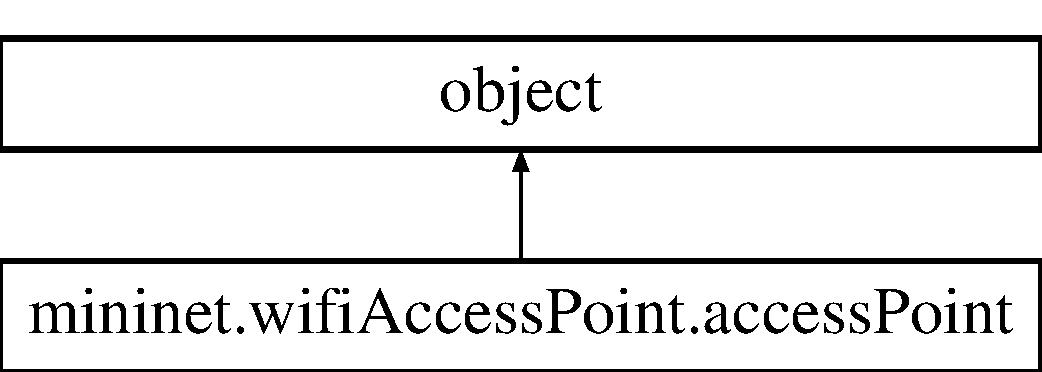
\includegraphics[height=2.000000cm]{classmininet_1_1wifiAccessPoint_1_1accessPoint}
\end{center}
\end{figure}
\subsection*{Public Member Functions}
\begin{DoxyCompactItemize}
\item 
\hypertarget{classmininet_1_1wifiAccessPoint_1_1accessPoint_a12e7868d8c55d9717687163ad5e95daf}{def {\bfseries \-\_\-\-\_\-init\-\_\-\-\_\-}}\label{classmininet_1_1wifiAccessPoint_1_1accessPoint_a12e7868d8c55d9717687163ad5e95daf}

\item 
\hypertarget{classmininet_1_1wifiAccessPoint_1_1accessPoint_a3cbec4757d89e8f3317726a73ac51350}{def {\bfseries rename\-Iface}}\label{classmininet_1_1wifiAccessPoint_1_1accessPoint_a3cbec4757d89e8f3317726a73ac51350}

\item 
def \hyperlink{classmininet_1_1wifiAccessPoint_1_1accessPoint_a925e7c762d13c896358ef4349b40aa65}{start}
\item 
def \hyperlink{classmininet_1_1wifiAccessPoint_1_1accessPoint_ae9d3adbb08daab476495ec53903560c8}{get\-Mac\-Address}
\item 
def \hyperlink{classmininet_1_1wifiAccessPoint_1_1accessPoint_a34e66b40e2ac3d09580f408b80289a41}{check\-Network\-Manager}
\item 
def \hyperlink{classmininet_1_1wifiAccessPoint_1_1accessPoint_adc20e2474f8f7822d2c3fbfee5aa6299}{ap\-Bridge}
\item 
def \hyperlink{classmininet_1_1wifiAccessPoint_1_1accessPoint_affd8f039b13b30a03aa84c59a93c2a20}{set\-Bw}
\item 
def \hyperlink{classmininet_1_1wifiAccessPoint_1_1accessPoint_ae3d5cced9fea44b92512a13c3d118c37}{A\-Pfile}
\end{DoxyCompactItemize}
\subsection*{Public Attributes}
\begin{DoxyCompactItemize}
\item 
\hypertarget{classmininet_1_1wifiAccessPoint_1_1accessPoint_a20057ad02224e80fcaa67868ab5f60a3}{{\bfseries cmd}}\label{classmininet_1_1wifiAccessPoint_1_1accessPoint_a20057ad02224e80fcaa67868ab5f60a3}

\item 
\hypertarget{classmininet_1_1wifiAccessPoint_1_1accessPoint_ae04725d76f113a3f5199607377d628ed}{{\bfseries print\-Mac}}\label{classmininet_1_1wifiAccessPoint_1_1accessPoint_ae04725d76f113a3f5199607377d628ed}

\item 
\hypertarget{classmininet_1_1wifiAccessPoint_1_1accessPoint_a5db7a34156843e0448717005af6a378c}{{\bfseries result\-Iface}}\label{classmininet_1_1wifiAccessPoint_1_1accessPoint_a5db7a34156843e0448717005af6a378c}

\end{DoxyCompactItemize}
\subsection*{Static Public Attributes}
\begin{DoxyCompactItemize}
\item 
\hypertarget{classmininet_1_1wifiAccessPoint_1_1accessPoint_a5a829add942982d08a12a19e7b914586}{{\bfseries wpa\-\_\-supplicant\-Is\-Running} = False}\label{classmininet_1_1wifiAccessPoint_1_1accessPoint_a5a829add942982d08a12a19e7b914586}

\end{DoxyCompactItemize}


\subsection{Member Function Documentation}
\hypertarget{classmininet_1_1wifiAccessPoint_1_1accessPoint_adc20e2474f8f7822d2c3fbfee5aa6299}{\index{mininet\-::wifi\-Access\-Point\-::access\-Point@{mininet\-::wifi\-Access\-Point\-::access\-Point}!ap\-Bridge@{ap\-Bridge}}
\index{ap\-Bridge@{ap\-Bridge}!mininet::wifiAccessPoint::accessPoint@{mininet\-::wifi\-Access\-Point\-::access\-Point}}
\subsubsection[{ap\-Bridge}]{\setlength{\rightskip}{0pt plus 5cm}def mininet.\-wifi\-Access\-Point.\-access\-Point.\-ap\-Bridge (
\begin{DoxyParamCaption}
\item[{}]{self, }
\item[{}]{ap, }
\item[{}]{iface}
\end{DoxyParamCaption}
)}}\label{classmininet_1_1wifiAccessPoint_1_1accessPoint_adc20e2474f8f7822d2c3fbfee5aa6299}
\begin{DoxyVerb}AP Bridge \end{DoxyVerb}
 \hypertarget{classmininet_1_1wifiAccessPoint_1_1accessPoint_ae3d5cced9fea44b92512a13c3d118c37}{\index{mininet\-::wifi\-Access\-Point\-::access\-Point@{mininet\-::wifi\-Access\-Point\-::access\-Point}!A\-Pfile@{A\-Pfile}}
\index{A\-Pfile@{A\-Pfile}!mininet::wifiAccessPoint::accessPoint@{mininet\-::wifi\-Access\-Point\-::access\-Point}}
\subsubsection[{A\-Pfile}]{\setlength{\rightskip}{0pt plus 5cm}def mininet.\-wifi\-Access\-Point.\-access\-Point.\-A\-Pfile (
\begin{DoxyParamCaption}
\item[{}]{self, }
\item[{}]{cmd, }
\item[{}]{ap, }
\item[{}]{wlan}
\end{DoxyParamCaption}
)}}\label{classmininet_1_1wifiAccessPoint_1_1accessPoint_ae3d5cced9fea44b92512a13c3d118c37}
\begin{DoxyVerb}run an Access Point and create the config file  \end{DoxyVerb}
 \hypertarget{classmininet_1_1wifiAccessPoint_1_1accessPoint_a34e66b40e2ac3d09580f408b80289a41}{\index{mininet\-::wifi\-Access\-Point\-::access\-Point@{mininet\-::wifi\-Access\-Point\-::access\-Point}!check\-Network\-Manager@{check\-Network\-Manager}}
\index{check\-Network\-Manager@{check\-Network\-Manager}!mininet::wifiAccessPoint::accessPoint@{mininet\-::wifi\-Access\-Point\-::access\-Point}}
\subsubsection[{check\-Network\-Manager}]{\setlength{\rightskip}{0pt plus 5cm}def mininet.\-wifi\-Access\-Point.\-access\-Point.\-check\-Network\-Manager (
\begin{DoxyParamCaption}
\item[{}]{self, }
\item[{}]{mac}
\end{DoxyParamCaption}
)}}\label{classmininet_1_1wifiAccessPoint_1_1accessPoint_a34e66b40e2ac3d09580f408b80289a41}
\begin{DoxyVerb}add mac address inside of /etc/NetworkManager/NetworkManager.conf \end{DoxyVerb}
 \hypertarget{classmininet_1_1wifiAccessPoint_1_1accessPoint_ae9d3adbb08daab476495ec53903560c8}{\index{mininet\-::wifi\-Access\-Point\-::access\-Point@{mininet\-::wifi\-Access\-Point\-::access\-Point}!get\-Mac\-Address@{get\-Mac\-Address}}
\index{get\-Mac\-Address@{get\-Mac\-Address}!mininet::wifiAccessPoint::accessPoint@{mininet\-::wifi\-Access\-Point\-::access\-Point}}
\subsubsection[{get\-Mac\-Address}]{\setlength{\rightskip}{0pt plus 5cm}def mininet.\-wifi\-Access\-Point.\-access\-Point.\-get\-Mac\-Address (
\begin{DoxyParamCaption}
\item[{}]{self, }
\item[{}]{ap, }
\item[{}]{wlan}
\end{DoxyParamCaption}
)}}\label{classmininet_1_1wifiAccessPoint_1_1accessPoint_ae9d3adbb08daab476495ec53903560c8}
\begin{DoxyVerb}get Mac Address of any Interface \end{DoxyVerb}
 \hypertarget{classmininet_1_1wifiAccessPoint_1_1accessPoint_affd8f039b13b30a03aa84c59a93c2a20}{\index{mininet\-::wifi\-Access\-Point\-::access\-Point@{mininet\-::wifi\-Access\-Point\-::access\-Point}!set\-Bw@{set\-Bw}}
\index{set\-Bw@{set\-Bw}!mininet::wifiAccessPoint::accessPoint@{mininet\-::wifi\-Access\-Point\-::access\-Point}}
\subsubsection[{set\-Bw}]{\setlength{\rightskip}{0pt plus 5cm}def mininet.\-wifi\-Access\-Point.\-access\-Point.\-set\-Bw (
\begin{DoxyParamCaption}
\item[{}]{self, }
\item[{}]{ap, }
\item[{}]{iface}
\end{DoxyParamCaption}
)}}\label{classmininet_1_1wifiAccessPoint_1_1accessPoint_affd8f039b13b30a03aa84c59a93c2a20}
\begin{DoxyVerb}Set bw to AP \end{DoxyVerb}
 \hypertarget{classmininet_1_1wifiAccessPoint_1_1accessPoint_a925e7c762d13c896358ef4349b40aa65}{\index{mininet\-::wifi\-Access\-Point\-::access\-Point@{mininet\-::wifi\-Access\-Point\-::access\-Point}!start@{start}}
\index{start@{start}!mininet::wifiAccessPoint::accessPoint@{mininet\-::wifi\-Access\-Point\-::access\-Point}}
\subsubsection[{start}]{\setlength{\rightskip}{0pt plus 5cm}def mininet.\-wifi\-Access\-Point.\-access\-Point.\-start (
\begin{DoxyParamCaption}
\item[{}]{self, }
\item[{}]{ap, }
\item[{}]{country\-\_\-code = {\ttfamily None}, }
\item[{}]{auth\-\_\-algs = {\ttfamily None}, }
\item[{}]{wpa = {\ttfamily None}, }
\item[{}]{wlan = {\ttfamily None}, }
\item[{}]{wpa\-\_\-key\-\_\-mgmt = {\ttfamily None}, }
\item[{}]{rsn\-\_\-pairwise = {\ttfamily None}, }
\item[{}]{wpa\-\_\-passphrase = {\ttfamily None}, }
\item[{}]{encrypt = {\ttfamily None}, }
\item[{}]{wep\-\_\-key0 = {\ttfamily None}, }
\item[{}]{params}
\end{DoxyParamCaption}
)}}\label{classmininet_1_1wifiAccessPoint_1_1accessPoint_a925e7c762d13c896358ef4349b40aa65}
\begin{DoxyVerb}Starts an Access Point \end{DoxyVerb}
 

The documentation for this class was generated from the following file\-:\begin{DoxyCompactItemize}
\item 
wifi\-Access\-Point.\-py\end{DoxyCompactItemize}

\hypertarget{classmininet_1_1wifiAssociation_1_1association}{\section{mininet.\-wifi\-Association.\-association Class Reference}
\label{classmininet_1_1wifiAssociation_1_1association}\index{mininet.\-wifi\-Association.\-association@{mininet.\-wifi\-Association.\-association}}
}
Inheritance diagram for mininet.\-wifi\-Association.\-association\-:\begin{figure}[H]
\begin{center}
\leavevmode
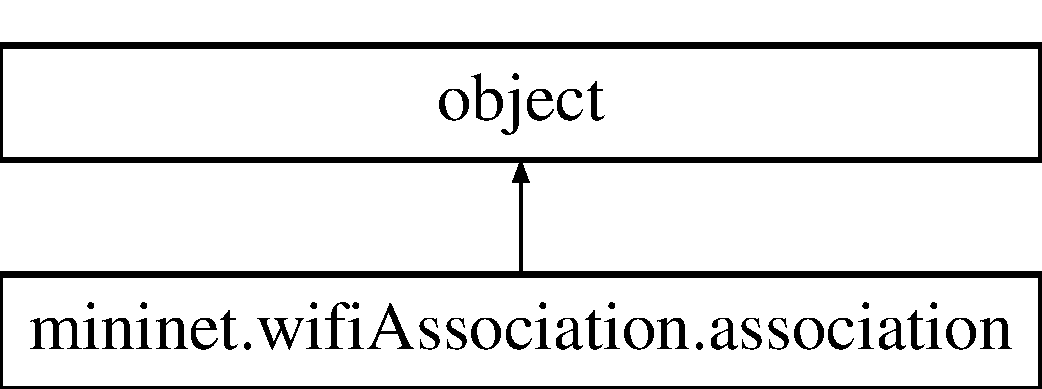
\includegraphics[height=2.000000cm]{classmininet_1_1wifiAssociation_1_1association}
\end{center}
\end{figure}
\subsection*{Public Member Functions}
\begin{DoxyCompactItemize}
\item 
\hypertarget{classmininet_1_1wifiAssociation_1_1association_aabf7b917eff483bde002bb810252ea38}{def {\bfseries confirm\-Infra\-Association}}\label{classmininet_1_1wifiAssociation_1_1association_aabf7b917eff483bde002bb810252ea38}

\item 
\hypertarget{classmininet_1_1wifiAssociation_1_1association_a4b2a30054b859b53ab84c1dad7026422}{def {\bfseries is\-Associated}}\label{classmininet_1_1wifiAssociation_1_1association_a4b2a30054b859b53ab84c1dad7026422}

\item 
\hypertarget{classmininet_1_1wifiAssociation_1_1association_a6e3168ea8c855dbf67cb19bbcad907eb}{def {\bfseries cmd\-\_\-associate}}\label{classmininet_1_1wifiAssociation_1_1association_a6e3168ea8c855dbf67cb19bbcad907eb}

\item 
\hypertarget{classmininet_1_1wifiAssociation_1_1association_a8b09f50615213610818686f9161f4ab4}{def {\bfseries associate\-\_\-wpa}}\label{classmininet_1_1wifiAssociation_1_1association_a8b09f50615213610818686f9161f4ab4}

\item 
\hypertarget{classmininet_1_1wifiAssociation_1_1association_a8099fe98b20c51de150b22b3a58124d0}{def {\bfseries associate\-\_\-wep}}\label{classmininet_1_1wifiAssociation_1_1association_a8099fe98b20c51de150b22b3a58124d0}

\end{DoxyCompactItemize}
\subsection*{Static Public Attributes}
\begin{DoxyCompactItemize}
\item 
\hypertarget{classmininet_1_1wifiAssociation_1_1association_a3fd340c4d41ae1896ec4c2f3f878a116}{{\bfseries print\-Con} = True}\label{classmininet_1_1wifiAssociation_1_1association_a3fd340c4d41ae1896ec4c2f3f878a116}

\item 
\hypertarget{classmininet_1_1wifiAssociation_1_1association_a0463e8bd7c7030afc3626dbc5184cb56}{{\bfseries is\-Code} = False}\label{classmininet_1_1wifiAssociation_1_1association_a0463e8bd7c7030afc3626dbc5184cb56}

\end{DoxyCompactItemize}


\subsection{Detailed Description}
\begin{DoxyVerb}Association Class\end{DoxyVerb}
 

The documentation for this class was generated from the following file\-:\begin{DoxyCompactItemize}
\item 
wifi\-Association.\-py\end{DoxyCompactItemize}

\hypertarget{classmininet_1_1wifiAssociationControl_1_1associationControl}{\section{mininet.\-wifi\-Association\-Control.\-association\-Control Class Reference}
\label{classmininet_1_1wifiAssociationControl_1_1associationControl}\index{mininet.\-wifi\-Association\-Control.\-association\-Control@{mininet.\-wifi\-Association\-Control.\-association\-Control}}
}
Inheritance diagram for mininet.\-wifi\-Association\-Control.\-association\-Control\-:\begin{figure}[H]
\begin{center}
\leavevmode
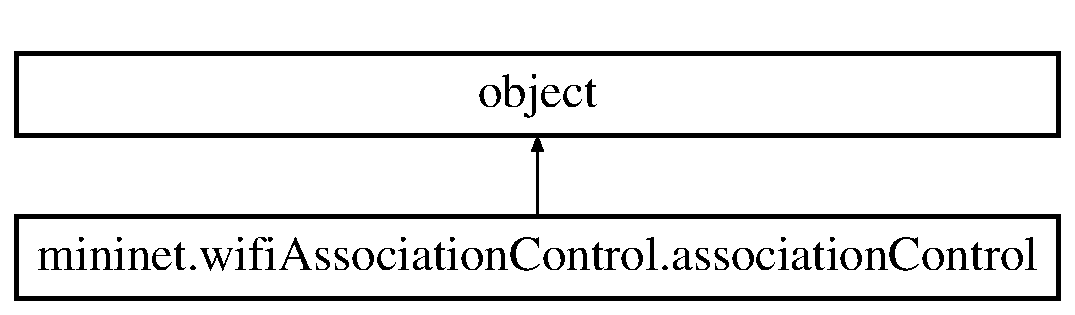
\includegraphics[height=2.000000cm]{classmininet_1_1wifiAssociationControl_1_1associationControl}
\end{center}
\end{figure}
\subsection*{Public Member Functions}
\begin{DoxyCompactItemize}
\item 
\hypertarget{classmininet_1_1wifiAssociationControl_1_1associationControl_ae0b486af6dc9b19651af1f0ac78c9351}{def {\bfseries \-\_\-\-\_\-init\-\_\-\-\_\-}}\label{classmininet_1_1wifiAssociationControl_1_1associationControl_ae0b486af6dc9b19651af1f0ac78c9351}

\item 
def \hyperlink{classmininet_1_1wifiAssociationControl_1_1associationControl_a816fb0f46f18bc39e4b25d6e22c95d39}{custom\-Association\-Control}
\end{DoxyCompactItemize}
\subsection*{Static Public Attributes}
\begin{DoxyCompactItemize}
\item 
\hypertarget{classmininet_1_1wifiAssociationControl_1_1associationControl_a93a998d27352625fcdd20034a57073be}{{\bfseries change\-A\-P} = False}\label{classmininet_1_1wifiAssociationControl_1_1associationControl_a93a998d27352625fcdd20034a57073be}

\end{DoxyCompactItemize}


\subsection{Member Function Documentation}
\hypertarget{classmininet_1_1wifiAssociationControl_1_1associationControl_a816fb0f46f18bc39e4b25d6e22c95d39}{\index{mininet\-::wifi\-Association\-Control\-::association\-Control@{mininet\-::wifi\-Association\-Control\-::association\-Control}!custom\-Association\-Control@{custom\-Association\-Control}}
\index{custom\-Association\-Control@{custom\-Association\-Control}!mininet::wifiAssociationControl::associationControl@{mininet\-::wifi\-Association\-Control\-::association\-Control}}
\subsubsection[{custom\-Association\-Control}]{\setlength{\rightskip}{0pt plus 5cm}def mininet.\-wifi\-Association\-Control.\-association\-Control.\-custom\-Association\-Control (
\begin{DoxyParamCaption}
\item[{}]{self, }
\item[{}]{node1, }
\item[{}]{node2, }
\item[{}]{wlan, }
\item[{}]{ac}
\end{DoxyParamCaption}
)}}\label{classmininet_1_1wifiAssociationControl_1_1associationControl_a816fb0f46f18bc39e4b25d6e22c95d39}
\begin{DoxyVerb}Mechanisms that optimize the use of the APs\end{DoxyVerb}
 

The documentation for this class was generated from the following file\-:\begin{DoxyCompactItemize}
\item 
wifi\-Association\-Control.\-py\end{DoxyCompactItemize}

\hypertarget{classmininet_1_1wifiChannel_1_1channelParameters}{\section{mininet.\-wifi\-Channel.\-channel\-Parameters Class Reference}
\label{classmininet_1_1wifiChannel_1_1channelParameters}\index{mininet.\-wifi\-Channel.\-channel\-Parameters@{mininet.\-wifi\-Channel.\-channel\-Parameters}}
}
Inheritance diagram for mininet.\-wifi\-Channel.\-channel\-Parameters\-:\begin{figure}[H]
\begin{center}
\leavevmode
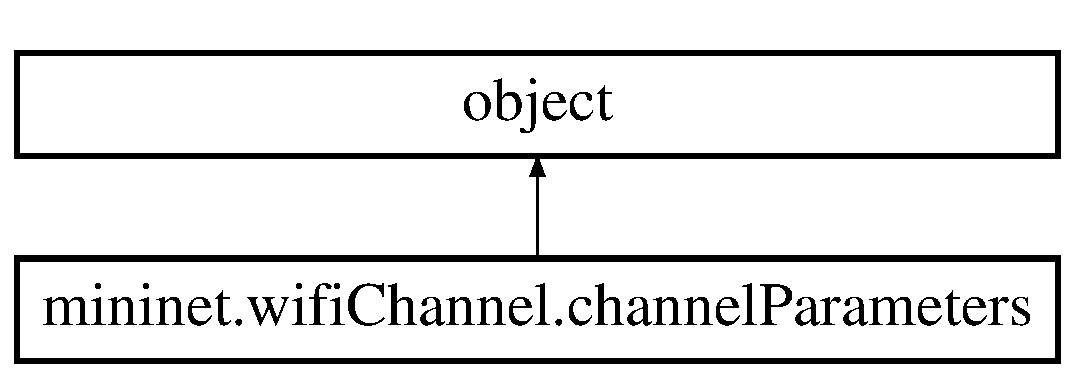
\includegraphics[height=2.000000cm]{classmininet_1_1wifiChannel_1_1channelParameters}
\end{center}
\end{figure}
\subsection*{Public Member Functions}
\begin{DoxyCompactItemize}
\item 
\hypertarget{classmininet_1_1wifiChannel_1_1channelParameters_a0022f742361108524c8d57c2ea42b83e}{def {\bfseries \-\_\-\-\_\-init\-\_\-\-\_\-}}\label{classmininet_1_1wifiChannel_1_1channelParameters_a0022f742361108524c8d57c2ea42b83e}

\item 
def \hyperlink{classmininet_1_1wifiChannel_1_1channelParameters_a1027487f6288c6256cd5b41b84b0c4c1}{get\-Distance}
\item 
def \hyperlink{classmininet_1_1wifiChannel_1_1channelParameters_a70ee0a55780d41c98d0d186aee3709f6}{delay}
\item 
\hypertarget{classmininet_1_1wifiChannel_1_1channelParameters_a3c3231b02dda6b85075f97242218106e}{def {\bfseries latency}}\label{classmininet_1_1wifiChannel_1_1channelParameters_a3c3231b02dda6b85075f97242218106e}

\item 
\hypertarget{classmininet_1_1wifiChannel_1_1channelParameters_a9599d6596c89d6130c58f1312f6f1b9b}{def {\bfseries loss}}\label{classmininet_1_1wifiChannel_1_1channelParameters_a9599d6596c89d6130c58f1312f6f1b9b}

\item 
\hypertarget{classmininet_1_1wifiChannel_1_1channelParameters_a7638cb6bebd58fe47f119ad09c74b4dc}{def {\bfseries bw}}\label{classmininet_1_1wifiChannel_1_1channelParameters_a7638cb6bebd58fe47f119ad09c74b4dc}

\item 
\hypertarget{classmininet_1_1wifiChannel_1_1channelParameters_ae431138dda16105dbf1e80852b836522}{def {\bfseries tc}}\label{classmininet_1_1wifiChannel_1_1channelParameters_ae431138dda16105dbf1e80852b836522}

\item 
\hypertarget{classmininet_1_1wifiChannel_1_1channelParameters_a83b7428940e0e4e9b4c044e6b4244dd9}{def {\bfseries calculate\-Interference}}\label{classmininet_1_1wifiChannel_1_1channelParameters_a83b7428940e0e4e9b4c044e6b4244dd9}

\item 
\hypertarget{classmininet_1_1wifiChannel_1_1channelParameters_a53ef24ba7eb7b348828d27567b294daf}{def {\bfseries calculate\-Noise}}\label{classmininet_1_1wifiChannel_1_1channelParameters_a53ef24ba7eb7b348828d27567b294daf}

\item 
def \hyperlink{classmininet_1_1wifiChannel_1_1channelParameters_a5cf19f9a021dd989f07199ac82ddecfb}{signal\-To\-Noise\-Ratio}
\item 
def \hyperlink{classmininet_1_1wifiChannel_1_1channelParameters_a637c3980e2f615a0793a54515c1bf766}{max\-Channel\-Noise}
\item 
def \hyperlink{classmininet_1_1wifiChannel_1_1channelParameters_a33ae91a9b837bc79e5591f33bbde451d}{link\-Margin}
\end{DoxyCompactItemize}
\subsection*{Public Attributes}
\begin{DoxyCompactItemize}
\item 
\hypertarget{classmininet_1_1wifiChannel_1_1channelParameters_a18d4bc7c6d3be6d3b569ef0e4fb7336e}{{\bfseries dist}}\label{classmininet_1_1wifiChannel_1_1channelParameters_a18d4bc7c6d3be6d3b569ef0e4fb7336e}

\item 
\hyperlink{classmininet_1_1wifiChannel_1_1channelParameters_a8b3099d0d44dd8c5f467936c4d1b9422}{delay}
\item 
\hypertarget{classmininet_1_1wifiChannel_1_1channelParameters_a296fa80d283f765f8dbbed78a2fbe613}{{\bfseries latency}}\label{classmininet_1_1wifiChannel_1_1channelParameters_a296fa80d283f765f8dbbed78a2fbe613}

\item 
\hypertarget{classmininet_1_1wifiChannel_1_1channelParameters_a9109efbf2aa2ec8539c0381e57e89d30}{{\bfseries loss}}\label{classmininet_1_1wifiChannel_1_1channelParameters_a9109efbf2aa2ec8539c0381e57e89d30}

\item 
\hypertarget{classmininet_1_1wifiChannel_1_1channelParameters_aa26df192b022976483bcd74777d535f6}{{\bfseries bw}}\label{classmininet_1_1wifiChannel_1_1channelParameters_aa26df192b022976483bcd74777d535f6}

\item 
\hypertarget{classmininet_1_1wifiChannel_1_1channelParameters_af596aad1d7a50801a60e4f724f9d9b09}{{\bfseries rate}}\label{classmininet_1_1wifiChannel_1_1channelParameters_af596aad1d7a50801a60e4f724f9d9b09}

\item 
\hypertarget{classmininet_1_1wifiChannel_1_1channelParameters_aa34488463cfc34b587ef7d204f233254}{{\bfseries noise}}\label{classmininet_1_1wifiChannel_1_1channelParameters_aa34488463cfc34b587ef7d204f233254}

\item 
\hypertarget{classmininet_1_1wifiChannel_1_1channelParameters_a4d4f6a5f02a88de6e31784fd502001ff}{{\bfseries i}}\label{classmininet_1_1wifiChannel_1_1channelParameters_a4d4f6a5f02a88de6e31784fd502001ff}

\end{DoxyCompactItemize}
\subsection*{Static Public Attributes}
\begin{DoxyCompactItemize}
\item 
\hypertarget{classmininet_1_1wifiChannel_1_1channelParameters_a0ea61ec1fa1243297a503abecd8695a2}{int {\bfseries delay} = 0}\label{classmininet_1_1wifiChannel_1_1channelParameters_a0ea61ec1fa1243297a503abecd8695a2}

\item 
\hypertarget{classmininet_1_1wifiChannel_1_1channelParameters_a5e741fb73b0ae594cce68fb5718a92b6}{int {\bfseries loss} = 0}\label{classmininet_1_1wifiChannel_1_1channelParameters_a5e741fb73b0ae594cce68fb5718a92b6}

\item 
\hypertarget{classmininet_1_1wifiChannel_1_1channelParameters_a1d8388c682f386919b36d85d69b16ec7}{int {\bfseries latency} = 0}\label{classmininet_1_1wifiChannel_1_1channelParameters_a1d8388c682f386919b36d85d69b16ec7}

\item 
\hypertarget{classmininet_1_1wifiChannel_1_1channelParameters_a90931cd3ce87f75886e4b3c87ba1b4f5}{int {\bfseries rate} = 0}\label{classmininet_1_1wifiChannel_1_1channelParameters_a90931cd3ce87f75886e4b3c87ba1b4f5}

\item 
\hypertarget{classmininet_1_1wifiChannel_1_1channelParameters_acc1e42e6b2368846e013a9ee5b88bf80}{int {\bfseries dist} = 0}\label{classmininet_1_1wifiChannel_1_1channelParameters_acc1e42e6b2368846e013a9ee5b88bf80}

\item 
\hypertarget{classmininet_1_1wifiChannel_1_1channelParameters_a10132fc554eac46d41136a6364b1e6da}{int {\bfseries noise} = 0}\label{classmininet_1_1wifiChannel_1_1channelParameters_a10132fc554eac46d41136a6364b1e6da}

\item 
\hypertarget{classmininet_1_1wifiChannel_1_1channelParameters_a60c5fac994a86c932d3d312ce26ed1d4}{int {\bfseries i} = 0}\label{classmininet_1_1wifiChannel_1_1channelParameters_a60c5fac994a86c932d3d312ce26ed1d4}

\end{DoxyCompactItemize}


\subsection{Detailed Description}
\begin{DoxyVerb}Channel Parameters\end{DoxyVerb}
 

\subsection{Member Function Documentation}
\hypertarget{classmininet_1_1wifiChannel_1_1channelParameters_a70ee0a55780d41c98d0d186aee3709f6}{\index{mininet\-::wifi\-Channel\-::channel\-Parameters@{mininet\-::wifi\-Channel\-::channel\-Parameters}!delay@{delay}}
\index{delay@{delay}!mininet::wifiChannel::channelParameters@{mininet\-::wifi\-Channel\-::channel\-Parameters}}
\subsubsection[{delay}]{\setlength{\rightskip}{0pt plus 5cm}def mininet.\-wifi\-Channel.\-channel\-Parameters.\-delay (
\begin{DoxyParamCaption}
\item[{}]{self, }
\item[{}]{dist, }
\item[{}]{time}
\end{DoxyParamCaption}
)}}\label{classmininet_1_1wifiChannel_1_1channelParameters_a70ee0a55780d41c98d0d186aee3709f6}
\begin{DoxyVerb}"Based on RandomPropagationDelayModel\end{DoxyVerb}
 \hypertarget{classmininet_1_1wifiChannel_1_1channelParameters_a1027487f6288c6256cd5b41b84b0c4c1}{\index{mininet\-::wifi\-Channel\-::channel\-Parameters@{mininet\-::wifi\-Channel\-::channel\-Parameters}!get\-Distance@{get\-Distance}}
\index{get\-Distance@{get\-Distance}!mininet::wifiChannel::channelParameters@{mininet\-::wifi\-Channel\-::channel\-Parameters}}
\subsubsection[{get\-Distance}]{\setlength{\rightskip}{0pt plus 5cm}def mininet.\-wifi\-Channel.\-channel\-Parameters.\-get\-Distance (
\begin{DoxyParamCaption}
\item[{}]{self, }
\item[{}]{src, }
\item[{}]{dst}
\end{DoxyParamCaption}
)}}\label{classmininet_1_1wifiChannel_1_1channelParameters_a1027487f6288c6256cd5b41b84b0c4c1}
\begin{DoxyVerb}Get the distance between two nodes \end{DoxyVerb}
 \hypertarget{classmininet_1_1wifiChannel_1_1channelParameters_a33ae91a9b837bc79e5591f33bbde451d}{\index{mininet\-::wifi\-Channel\-::channel\-Parameters@{mininet\-::wifi\-Channel\-::channel\-Parameters}!link\-Margin@{link\-Margin}}
\index{link\-Margin@{link\-Margin}!mininet::wifiChannel::channelParameters@{mininet\-::wifi\-Channel\-::channel\-Parameters}}
\subsubsection[{link\-Margin}]{\setlength{\rightskip}{0pt plus 5cm}def mininet.\-wifi\-Channel.\-channel\-Parameters.\-link\-Margin (
\begin{DoxyParamCaption}
\item[{}]{self, }
\item[{}]{node1, }
\item[{}]{node2, }
\item[{}]{wlan, }
\item[{}]{model\-Value}
\end{DoxyParamCaption}
)}}\label{classmininet_1_1wifiChannel_1_1channelParameters_a33ae91a9b837bc79e5591f33bbde451d}
\begin{DoxyVerb}Have to work\end{DoxyVerb}
 \hypertarget{classmininet_1_1wifiChannel_1_1channelParameters_a637c3980e2f615a0793a54515c1bf766}{\index{mininet\-::wifi\-Channel\-::channel\-Parameters@{mininet\-::wifi\-Channel\-::channel\-Parameters}!max\-Channel\-Noise@{max\-Channel\-Noise}}
\index{max\-Channel\-Noise@{max\-Channel\-Noise}!mininet::wifiChannel::channelParameters@{mininet\-::wifi\-Channel\-::channel\-Parameters}}
\subsubsection[{max\-Channel\-Noise}]{\setlength{\rightskip}{0pt plus 5cm}def mininet.\-wifi\-Channel.\-channel\-Parameters.\-max\-Channel\-Noise (
\begin{DoxyParamCaption}
\item[{}]{self, }
\item[{}]{node1, }
\item[{}]{node2, }
\item[{}]{wlan, }
\item[{}]{model\-Value}
\end{DoxyParamCaption}
)}}\label{classmininet_1_1wifiChannel_1_1channelParameters_a637c3980e2f615a0793a54515c1bf766}
\begin{DoxyVerb}Have to work\end{DoxyVerb}
 \hypertarget{classmininet_1_1wifiChannel_1_1channelParameters_a5cf19f9a021dd989f07199ac82ddecfb}{\index{mininet\-::wifi\-Channel\-::channel\-Parameters@{mininet\-::wifi\-Channel\-::channel\-Parameters}!signal\-To\-Noise\-Ratio@{signal\-To\-Noise\-Ratio}}
\index{signal\-To\-Noise\-Ratio@{signal\-To\-Noise\-Ratio}!mininet::wifiChannel::channelParameters@{mininet\-::wifi\-Channel\-::channel\-Parameters}}
\subsubsection[{signal\-To\-Noise\-Ratio}]{\setlength{\rightskip}{0pt plus 5cm}def mininet.\-wifi\-Channel.\-channel\-Parameters.\-signal\-To\-Noise\-Ratio (
\begin{DoxyParamCaption}
\item[{}]{self, }
\item[{}]{signal\-Power, }
\item[{}]{noise\-Power}
\end{DoxyParamCaption}
)}}\label{classmininet_1_1wifiChannel_1_1channelParameters_a5cf19f9a021dd989f07199ac82ddecfb}
\begin{DoxyVerb}Calculating SNR margin\end{DoxyVerb}
 

\subsection{Member Data Documentation}
\hypertarget{classmininet_1_1wifiChannel_1_1channelParameters_a8b3099d0d44dd8c5f467936c4d1b9422}{\index{mininet\-::wifi\-Channel\-::channel\-Parameters@{mininet\-::wifi\-Channel\-::channel\-Parameters}!delay@{delay}}
\index{delay@{delay}!mininet::wifiChannel::channelParameters@{mininet\-::wifi\-Channel\-::channel\-Parameters}}
\subsubsection[{delay}]{\setlength{\rightskip}{0pt plus 5cm}mininet.\-wifi\-Channel.\-channel\-Parameters.\-delay}}\label{classmininet_1_1wifiChannel_1_1channelParameters_a8b3099d0d44dd8c5f467936c4d1b9422}
\begin{DoxyVerb}"Based on RandomPropagationDelayModel\end{DoxyVerb}
 

The documentation for this class was generated from the following file\-:\begin{DoxyCompactItemize}
\item 
wifi\-Channel.\-py\end{DoxyCompactItemize}

\hypertarget{classmininet_1_1clean_1_1Cleanup}{\section{mininet.\-clean.\-Cleanup Class Reference}
\label{classmininet_1_1clean_1_1Cleanup}\index{mininet.\-clean.\-Cleanup@{mininet.\-clean.\-Cleanup}}
}
Inheritance diagram for mininet.\-clean.\-Cleanup\-:\begin{figure}[H]
\begin{center}
\leavevmode
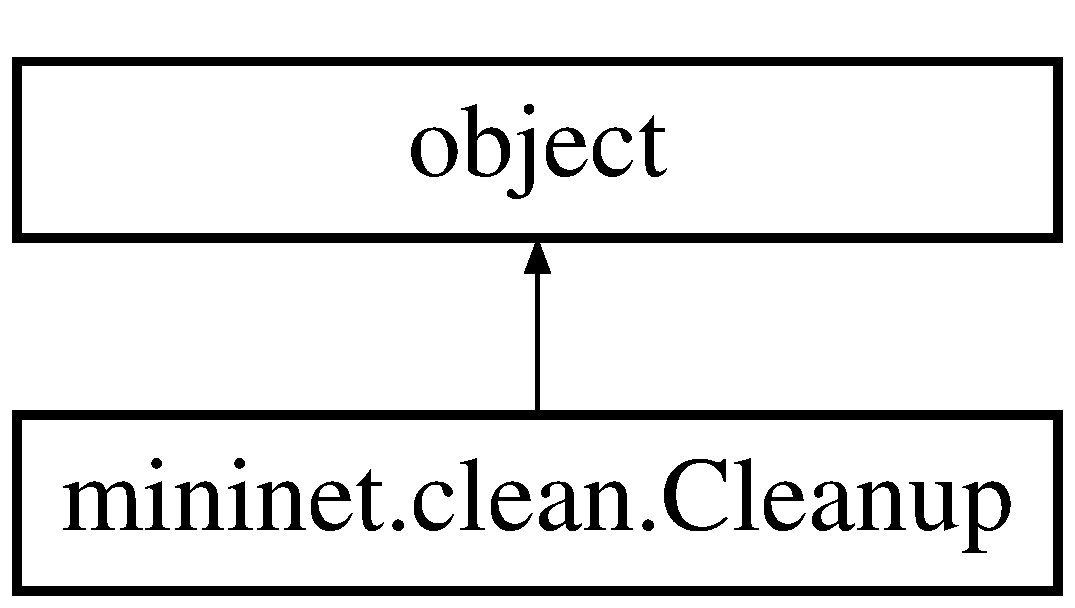
\includegraphics[height=2.000000cm]{classmininet_1_1clean_1_1Cleanup}
\end{center}
\end{figure}
\subsection*{Public Member Functions}
\begin{DoxyCompactItemize}
\item 
def \hyperlink{classmininet_1_1clean_1_1Cleanup_a699dbbb0f34039c95cda957d8580f181}{cleanup}
\item 
\hypertarget{classmininet_1_1clean_1_1Cleanup_a3746bdef3ce1e10f8a68fe93cdc1feb4}{def {\bfseries add\-Cleanup\-Callback}}\label{classmininet_1_1clean_1_1Cleanup_a3746bdef3ce1e10f8a68fe93cdc1feb4}

\end{DoxyCompactItemize}
\subsection*{Static Public Attributes}
\begin{DoxyCompactItemize}
\item 
\hypertarget{classmininet_1_1clean_1_1Cleanup_a82f1333f11a86d7b1be0da787660e9c3}{list {\bfseries callbacks} = \mbox{[}$\,$\mbox{]}}\label{classmininet_1_1clean_1_1Cleanup_a82f1333f11a86d7b1be0da787660e9c3}

\end{DoxyCompactItemize}


\subsection{Member Function Documentation}
\hypertarget{classmininet_1_1clean_1_1Cleanup_a699dbbb0f34039c95cda957d8580f181}{\index{mininet\-::clean\-::\-Cleanup@{mininet\-::clean\-::\-Cleanup}!cleanup@{cleanup}}
\index{cleanup@{cleanup}!mininet::clean::Cleanup@{mininet\-::clean\-::\-Cleanup}}
\subsubsection[{cleanup}]{\setlength{\rightskip}{0pt plus 5cm}def mininet.\-clean.\-Cleanup.\-cleanup (
\begin{DoxyParamCaption}
\item[{}]{cls}
\end{DoxyParamCaption}
)}}\label{classmininet_1_1clean_1_1Cleanup_a699dbbb0f34039c95cda957d8580f181}
\begin{DoxyVerb}Clean up junk which might be left over from old runs;
   do fast stuff before slow dp and link removal!\end{DoxyVerb}
 

The documentation for this class was generated from the following file\-:\begin{DoxyCompactItemize}
\item 
clean.\-py\end{DoxyCompactItemize}

\hypertarget{classmininet_1_1cli_1_1CLI}{\section{mininet.\-cli.\-C\-L\-I Class Reference}
\label{classmininet_1_1cli_1_1CLI}\index{mininet.\-cli.\-C\-L\-I@{mininet.\-cli.\-C\-L\-I}}
}
Inheritance diagram for mininet.\-cli.\-C\-L\-I\-:\begin{figure}[H]
\begin{center}
\leavevmode
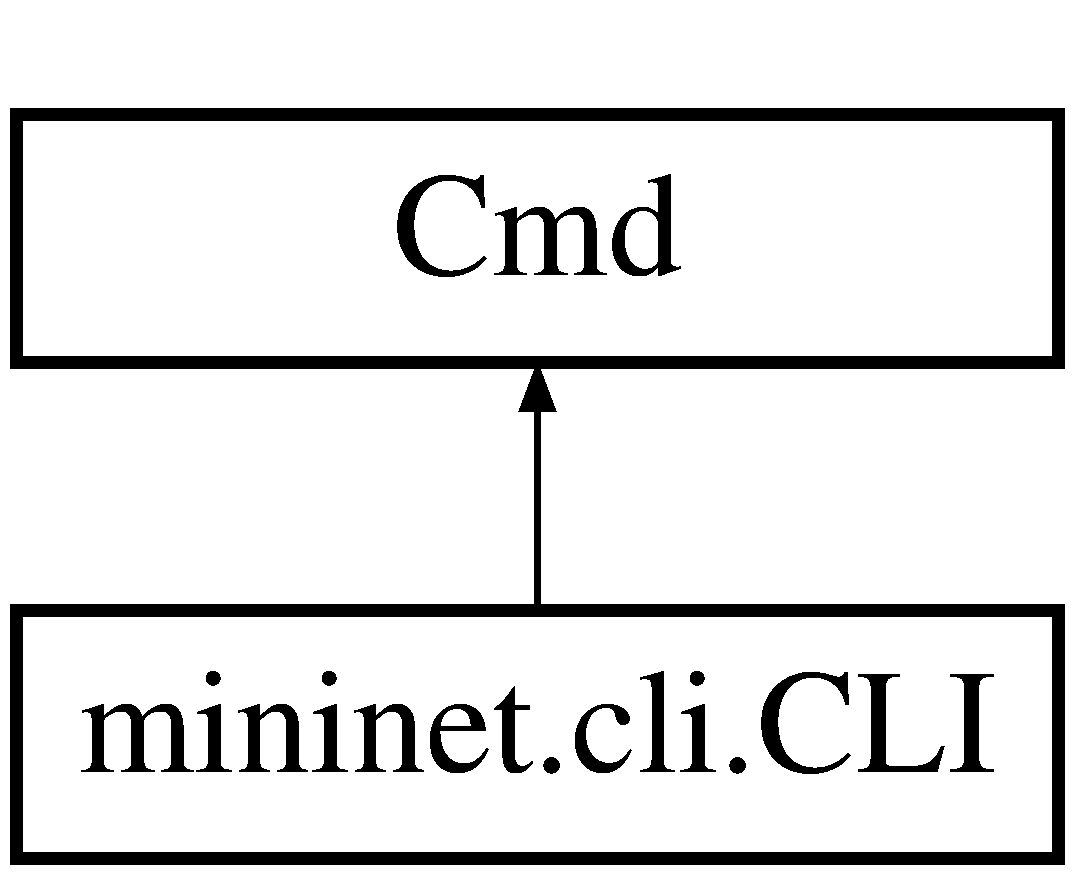
\includegraphics[height=2.000000cm]{classmininet_1_1cli_1_1CLI}
\end{center}
\end{figure}
\subsection*{Public Member Functions}
\begin{DoxyCompactItemize}
\item 
def \hyperlink{classmininet_1_1cli_1_1CLI_a8a7159a07a77a05fd9fa083d212f3012}{\-\_\-\-\_\-init\-\_\-\-\_\-}
\item 
\hypertarget{classmininet_1_1cli_1_1CLI_acb783f2a3affc84260cce2d5090260e0}{def {\bfseries init\-Readline}}\label{classmininet_1_1cli_1_1CLI_acb783f2a3affc84260cce2d5090260e0}

\item 
\hypertarget{classmininet_1_1cli_1_1CLI_a3d7edb1ba3b4635527f07823d2b1bcca}{def {\bfseries run}}\label{classmininet_1_1cli_1_1CLI_a3d7edb1ba3b4635527f07823d2b1bcca}

\item 
\hypertarget{classmininet_1_1cli_1_1CLI_a3c69fb5b0a23d1fdf59ae2a768561be3}{def {\bfseries emptyline}}\label{classmininet_1_1cli_1_1CLI_a3c69fb5b0a23d1fdf59ae2a768561be3}

\item 
\hypertarget{classmininet_1_1cli_1_1CLI_ab1617010c175d74b86f034091fe65c90}{def {\bfseries get\-Locals}}\label{classmininet_1_1cli_1_1CLI_ab1617010c175d74b86f034091fe65c90}

\item 
\hypertarget{classmininet_1_1cli_1_1CLI_adb2ea450f367d3a480ab4b1e70e60a78}{def {\bfseries do\-\_\-help}}\label{classmininet_1_1cli_1_1CLI_adb2ea450f367d3a480ab4b1e70e60a78}

\item 
\hypertarget{classmininet_1_1cli_1_1CLI_a25ae0fcb8e3538bdd93dbab7e0b59ee1}{def {\bfseries do\-\_\-nodes}}\label{classmininet_1_1cli_1_1CLI_a25ae0fcb8e3538bdd93dbab7e0b59ee1}

\item 
\hypertarget{classmininet_1_1cli_1_1CLI_aa63c97091c9ad85695de96046661f123}{def {\bfseries do\-\_\-ports}}\label{classmininet_1_1cli_1_1CLI_aa63c97091c9ad85695de96046661f123}

\item 
\hypertarget{classmininet_1_1cli_1_1CLI_a96a020a13653c2b4e504c270a560bd98}{def {\bfseries do\-\_\-net}}\label{classmininet_1_1cli_1_1CLI_a96a020a13653c2b4e504c270a560bd98}

\item 
def \hyperlink{classmininet_1_1cli_1_1CLI_a4df722296f69ca6f19f8fd89ea225042}{do\-\_\-sh}
\item 
def \hyperlink{classmininet_1_1cli_1_1CLI_abaee39bdb77c8ba35182e27a6e12d0a1}{do\-\_\-py}
\item 
def \hyperlink{classmininet_1_1cli_1_1CLI_ad4f829fe3e8105087a9f8a94b1fa05e9}{do\-\_\-px}
\item 
\hypertarget{classmininet_1_1cli_1_1CLI_a678d2542cce2e80baedb1bd7cece9a15}{def {\bfseries do\-\_\-pingall}}\label{classmininet_1_1cli_1_1CLI_a678d2542cce2e80baedb1bd7cece9a15}

\item 
\hypertarget{classmininet_1_1cli_1_1CLI_a1585a9578b466b58be93df5c2287de29}{def {\bfseries do\-\_\-pingpair}}\label{classmininet_1_1cli_1_1CLI_a1585a9578b466b58be93df5c2287de29}

\item 
\hypertarget{classmininet_1_1cli_1_1CLI_a8c329faf830234b55c2ee65f60bb0a8c}{def {\bfseries do\-\_\-pingallfull}}\label{classmininet_1_1cli_1_1CLI_a8c329faf830234b55c2ee65f60bb0a8c}

\item 
\hypertarget{classmininet_1_1cli_1_1CLI_a6b3fbb656d2aad4d6415b9126b8b3294}{def {\bfseries do\-\_\-pingpairfull}}\label{classmininet_1_1cli_1_1CLI_a6b3fbb656d2aad4d6415b9126b8b3294}

\item 
def \hyperlink{classmininet_1_1cli_1_1CLI_aa6d32352e3716b57ab3ee2b67ad874de}{do\-\_\-iperf}
\item 
def \hyperlink{classmininet_1_1cli_1_1CLI_ac549ff5bfc3452cc40a75a0a2b3c6796}{do\-\_\-iperfudp}
\item 
\hypertarget{classmininet_1_1cli_1_1CLI_ad55dcfafa41e93f58876370044be9e2e}{def {\bfseries do\-\_\-intfs}}\label{classmininet_1_1cli_1_1CLI_ad55dcfafa41e93f58876370044be9e2e}

\item 
\hypertarget{classmininet_1_1cli_1_1CLI_af8dd33475e2bdadf0b2112e54de93516}{def {\bfseries do\-\_\-dump}}\label{classmininet_1_1cli_1_1CLI_af8dd33475e2bdadf0b2112e54de93516}

\item 
\hypertarget{classmininet_1_1cli_1_1CLI_ac52cb6f29299a71a099f1329b0780c14}{def {\bfseries do\-\_\-info}}\label{classmininet_1_1cli_1_1CLI_ac52cb6f29299a71a099f1329b0780c14}

\item 
\hypertarget{classmininet_1_1cli_1_1CLI_a23505ebf0eae43cd8bac98f64a778d72}{def {\bfseries do\-\_\-distance}}\label{classmininet_1_1cli_1_1CLI_a23505ebf0eae43cd8bac98f64a778d72}

\item 
\hypertarget{classmininet_1_1cli_1_1CLI_a2c336269bc9905b012b1e1b9167314bd}{def {\bfseries do\-\_\-position}}\label{classmininet_1_1cli_1_1CLI_a2c336269bc9905b012b1e1b9167314bd}

\item 
def \hyperlink{classmininet_1_1cli_1_1CLI_a266fde03f66eee288021fa2a763afa3c}{do\-\_\-link}
\item 
def \hyperlink{classmininet_1_1cli_1_1CLI_a64f351dbb4a15c05ede169046b0d8a76}{do\-\_\-xterm}
\item 
def \hyperlink{classmininet_1_1cli_1_1CLI_a4a914a9c24fc11fe529d1adb8c287d77}{do\-\_\-x}
\item 
def \hyperlink{classmininet_1_1cli_1_1CLI_a0e441b6c7cf0b019a57510937d580240}{do\-\_\-gterm}
\item 
\hypertarget{classmininet_1_1cli_1_1CLI_a0320f70df0d8a6c03c12ede8b43ca803}{def {\bfseries do\-\_\-exit}}\label{classmininet_1_1cli_1_1CLI_a0320f70df0d8a6c03c12ede8b43ca803}

\item 
\hypertarget{classmininet_1_1cli_1_1CLI_af6cf376279a11581d2a18a206e2223df}{def {\bfseries do\-\_\-quit}}\label{classmininet_1_1cli_1_1CLI_af6cf376279a11581d2a18a206e2223df}

\item 
\hypertarget{classmininet_1_1cli_1_1CLI_abc45964b158b175f5c3a2939ced05d45}{def {\bfseries do\-\_\-\-E\-O\-F}}\label{classmininet_1_1cli_1_1CLI_abc45964b158b175f5c3a2939ced05d45}

\item 
\hypertarget{classmininet_1_1cli_1_1CLI_a45d1c906a6455bbce6c2a56bac7e5898}{def {\bfseries isatty}}\label{classmininet_1_1cli_1_1CLI_a45d1c906a6455bbce6c2a56bac7e5898}

\item 
def \hyperlink{classmininet_1_1cli_1_1CLI_a6e222dea35c2228bed883eb5fb1422a4}{do\-\_\-noecho}
\item 
def \hyperlink{classmininet_1_1cli_1_1CLI_a7a3d544358d43da59c26a5a522be7883}{do\-\_\-source}
\item 
def \hyperlink{classmininet_1_1cli_1_1CLI_a587dbea79c66cd416d3abfabe16af077}{do\-\_\-dpctl}
\item 
\hypertarget{classmininet_1_1cli_1_1CLI_abde313aec3fceeb8c6bddc19ad6cc528}{def {\bfseries do\-\_\-time}}\label{classmininet_1_1cli_1_1CLI_abde313aec3fceeb8c6bddc19ad6cc528}

\item 
\hypertarget{classmininet_1_1cli_1_1CLI_aa9482fa91fac9560897003737b846faf}{def {\bfseries do\-\_\-links}}\label{classmininet_1_1cli_1_1CLI_aa9482fa91fac9560897003737b846faf}

\item 
\hypertarget{classmininet_1_1cli_1_1CLI_ac771d28f773966e8a847bf7e8c407c4b}{def {\bfseries do\-\_\-switch}}\label{classmininet_1_1cli_1_1CLI_ac771d28f773966e8a847bf7e8c407c4b}

\item 
def \hyperlink{classmininet_1_1cli_1_1CLI_abb60fa854de8ad7d98f0cde4c35605d8}{default}
\item 
\hypertarget{classmininet_1_1cli_1_1CLI_a8d2bb34caf60529b295b8f5c477ee37e}{def {\bfseries wait\-For\-Node}}\label{classmininet_1_1cli_1_1CLI_a8d2bb34caf60529b295b8f5c477ee37e}

\item 
\hypertarget{classmininet_1_1cli_1_1CLI_a9cae6d145ab8bb8d2dcf36ac9d3866e1}{def {\bfseries precmd}}\label{classmininet_1_1cli_1_1CLI_a9cae6d145ab8bb8d2dcf36ac9d3866e1}

\end{DoxyCompactItemize}
\subsection*{Public Attributes}
\begin{DoxyCompactItemize}
\item 
\hypertarget{classmininet_1_1cli_1_1CLI_a0126b20d4775a134b1e06e591af3f05e}{{\bfseries mn}}\label{classmininet_1_1cli_1_1CLI_a0126b20d4775a134b1e06e591af3f05e}

\item 
\hypertarget{classmininet_1_1cli_1_1CLI_a7594e2ff92c24a6b1d24ad891acdf74f}{{\bfseries locals}}\label{classmininet_1_1cli_1_1CLI_a7594e2ff92c24a6b1d24ad891acdf74f}

\item 
\hypertarget{classmininet_1_1cli_1_1CLI_aebbab6e46fd3edc1ea8b2cfff39ce12c}{{\bfseries stdin}}\label{classmininet_1_1cli_1_1CLI_aebbab6e46fd3edc1ea8b2cfff39ce12c}

\item 
\hypertarget{classmininet_1_1cli_1_1CLI_ad5509db5a4e78c91f5f9b7da53693690}{{\bfseries in\-Poller}}\label{classmininet_1_1cli_1_1CLI_ad5509db5a4e78c91f5f9b7da53693690}

\item 
\hypertarget{classmininet_1_1cli_1_1CLI_afa57f558f8e90790a94d325af8db5818}{{\bfseries input\-File}}\label{classmininet_1_1cli_1_1CLI_afa57f558f8e90790a94d325af8db5818}

\end{DoxyCompactItemize}
\subsection*{Static Public Attributes}
\begin{DoxyCompactItemize}
\item 
\hypertarget{classmininet_1_1cli_1_1CLI_a343818ddcc27d8942a1316156c1f246c}{string {\bfseries prompt} = 'mininet-\/wifi$>$ '}\label{classmininet_1_1cli_1_1CLI_a343818ddcc27d8942a1316156c1f246c}

\item 
\hypertarget{classmininet_1_1cli_1_1CLI_a7fee306d59e2df221b8e7f7a9c189737}{{\bfseries readline\-Inited} = False}\label{classmininet_1_1cli_1_1CLI_a7fee306d59e2df221b8e7f7a9c189737}

\item 
tuple {\bfseries help\-Str}
\end{DoxyCompactItemize}


\subsection{Constructor \& Destructor Documentation}
\hypertarget{classmininet_1_1cli_1_1CLI_a8a7159a07a77a05fd9fa083d212f3012}{\index{mininet\-::cli\-::\-C\-L\-I@{mininet\-::cli\-::\-C\-L\-I}!\-\_\-\-\_\-init\-\_\-\-\_\-@{\-\_\-\-\_\-init\-\_\-\-\_\-}}
\index{\-\_\-\-\_\-init\-\_\-\-\_\-@{\-\_\-\-\_\-init\-\_\-\-\_\-}!mininet::cli::CLI@{mininet\-::cli\-::\-C\-L\-I}}
\subsubsection[{\-\_\-\-\_\-init\-\_\-\-\_\-}]{\setlength{\rightskip}{0pt plus 5cm}def mininet.\-cli.\-C\-L\-I.\-\_\-\-\_\-init\-\_\-\-\_\- (
\begin{DoxyParamCaption}
\item[{}]{self, }
\item[{}]{mininet, }
\item[{}]{stdin = {\ttfamily sys.stdin}, }
\item[{}]{script = {\ttfamily None}}
\end{DoxyParamCaption}
)}}\label{classmininet_1_1cli_1_1CLI_a8a7159a07a77a05fd9fa083d212f3012}
\begin{DoxyVerb}Start and run interactive or batch mode CLI
   mininet: Mininet network object
   stdin: standard input for CLI
   script: script to run in batch mode\end{DoxyVerb}
 

\subsection{Member Function Documentation}
\hypertarget{classmininet_1_1cli_1_1CLI_abb60fa854de8ad7d98f0cde4c35605d8}{\index{mininet\-::cli\-::\-C\-L\-I@{mininet\-::cli\-::\-C\-L\-I}!default@{default}}
\index{default@{default}!mininet::cli::CLI@{mininet\-::cli\-::\-C\-L\-I}}
\subsubsection[{default}]{\setlength{\rightskip}{0pt plus 5cm}def mininet.\-cli.\-C\-L\-I.\-default (
\begin{DoxyParamCaption}
\item[{}]{self, }
\item[{}]{line}
\end{DoxyParamCaption}
)}}\label{classmininet_1_1cli_1_1CLI_abb60fa854de8ad7d98f0cde4c35605d8}
\begin{DoxyVerb}Called on an input line when the command prefix is not recognized.
Overridden to run shell commands when a node is the first CLI argument.
Past the first CLI argument, node names are automatically replaced with
corresponding IP addrs.\end{DoxyVerb}
 \hypertarget{classmininet_1_1cli_1_1CLI_a587dbea79c66cd416d3abfabe16af077}{\index{mininet\-::cli\-::\-C\-L\-I@{mininet\-::cli\-::\-C\-L\-I}!do\-\_\-dpctl@{do\-\_\-dpctl}}
\index{do\-\_\-dpctl@{do\-\_\-dpctl}!mininet::cli::CLI@{mininet\-::cli\-::\-C\-L\-I}}
\subsubsection[{do\-\_\-dpctl}]{\setlength{\rightskip}{0pt plus 5cm}def mininet.\-cli.\-C\-L\-I.\-do\-\_\-dpctl (
\begin{DoxyParamCaption}
\item[{}]{self, }
\item[{}]{line}
\end{DoxyParamCaption}
)}}\label{classmininet_1_1cli_1_1CLI_a587dbea79c66cd416d3abfabe16af077}
\begin{DoxyVerb}Run dpctl (or ovs-ofctl) command on all switches.
   Usage: dpctl command [arg1] [arg2] ...\end{DoxyVerb}
 \hypertarget{classmininet_1_1cli_1_1CLI_a0e441b6c7cf0b019a57510937d580240}{\index{mininet\-::cli\-::\-C\-L\-I@{mininet\-::cli\-::\-C\-L\-I}!do\-\_\-gterm@{do\-\_\-gterm}}
\index{do\-\_\-gterm@{do\-\_\-gterm}!mininet::cli::CLI@{mininet\-::cli\-::\-C\-L\-I}}
\subsubsection[{do\-\_\-gterm}]{\setlength{\rightskip}{0pt plus 5cm}def mininet.\-cli.\-C\-L\-I.\-do\-\_\-gterm (
\begin{DoxyParamCaption}
\item[{}]{self, }
\item[{}]{line}
\end{DoxyParamCaption}
)}}\label{classmininet_1_1cli_1_1CLI_a0e441b6c7cf0b019a57510937d580240}
\begin{DoxyVerb}Spawn gnome-terminal(s) for the given node(s).
   Usage: gterm node1 node2 ...\end{DoxyVerb}
 \hypertarget{classmininet_1_1cli_1_1CLI_aa6d32352e3716b57ab3ee2b67ad874de}{\index{mininet\-::cli\-::\-C\-L\-I@{mininet\-::cli\-::\-C\-L\-I}!do\-\_\-iperf@{do\-\_\-iperf}}
\index{do\-\_\-iperf@{do\-\_\-iperf}!mininet::cli::CLI@{mininet\-::cli\-::\-C\-L\-I}}
\subsubsection[{do\-\_\-iperf}]{\setlength{\rightskip}{0pt plus 5cm}def mininet.\-cli.\-C\-L\-I.\-do\-\_\-iperf (
\begin{DoxyParamCaption}
\item[{}]{self, }
\item[{}]{line}
\end{DoxyParamCaption}
)}}\label{classmininet_1_1cli_1_1CLI_aa6d32352e3716b57ab3ee2b67ad874de}
\begin{DoxyVerb}Simple iperf TCP test between two (optionally specified) hosts.
   Usage: iperf node1 node2\end{DoxyVerb}
 \hypertarget{classmininet_1_1cli_1_1CLI_ac549ff5bfc3452cc40a75a0a2b3c6796}{\index{mininet\-::cli\-::\-C\-L\-I@{mininet\-::cli\-::\-C\-L\-I}!do\-\_\-iperfudp@{do\-\_\-iperfudp}}
\index{do\-\_\-iperfudp@{do\-\_\-iperfudp}!mininet::cli::CLI@{mininet\-::cli\-::\-C\-L\-I}}
\subsubsection[{do\-\_\-iperfudp}]{\setlength{\rightskip}{0pt plus 5cm}def mininet.\-cli.\-C\-L\-I.\-do\-\_\-iperfudp (
\begin{DoxyParamCaption}
\item[{}]{self, }
\item[{}]{line}
\end{DoxyParamCaption}
)}}\label{classmininet_1_1cli_1_1CLI_ac549ff5bfc3452cc40a75a0a2b3c6796}
\begin{DoxyVerb}Simple iperf UDP test between two (optionally specified) hosts.
   Usage: iperfudp bw node1 node2\end{DoxyVerb}
 \hypertarget{classmininet_1_1cli_1_1CLI_a266fde03f66eee288021fa2a763afa3c}{\index{mininet\-::cli\-::\-C\-L\-I@{mininet\-::cli\-::\-C\-L\-I}!do\-\_\-link@{do\-\_\-link}}
\index{do\-\_\-link@{do\-\_\-link}!mininet::cli::CLI@{mininet\-::cli\-::\-C\-L\-I}}
\subsubsection[{do\-\_\-link}]{\setlength{\rightskip}{0pt plus 5cm}def mininet.\-cli.\-C\-L\-I.\-do\-\_\-link (
\begin{DoxyParamCaption}
\item[{}]{self, }
\item[{}]{line}
\end{DoxyParamCaption}
)}}\label{classmininet_1_1cli_1_1CLI_a266fde03f66eee288021fa2a763afa3c}
\begin{DoxyVerb}Bring link(s) between two nodes up or down.
   Usage: link node1 node2 [up/down]\end{DoxyVerb}
 \hypertarget{classmininet_1_1cli_1_1CLI_a6e222dea35c2228bed883eb5fb1422a4}{\index{mininet\-::cli\-::\-C\-L\-I@{mininet\-::cli\-::\-C\-L\-I}!do\-\_\-noecho@{do\-\_\-noecho}}
\index{do\-\_\-noecho@{do\-\_\-noecho}!mininet::cli::CLI@{mininet\-::cli\-::\-C\-L\-I}}
\subsubsection[{do\-\_\-noecho}]{\setlength{\rightskip}{0pt plus 5cm}def mininet.\-cli.\-C\-L\-I.\-do\-\_\-noecho (
\begin{DoxyParamCaption}
\item[{}]{self, }
\item[{}]{line}
\end{DoxyParamCaption}
)}}\label{classmininet_1_1cli_1_1CLI_a6e222dea35c2228bed883eb5fb1422a4}
\begin{DoxyVerb}Run an interactive command with echoing turned off.
   Usage: noecho [cmd args]\end{DoxyVerb}
 \hypertarget{classmininet_1_1cli_1_1CLI_ad4f829fe3e8105087a9f8a94b1fa05e9}{\index{mininet\-::cli\-::\-C\-L\-I@{mininet\-::cli\-::\-C\-L\-I}!do\-\_\-px@{do\-\_\-px}}
\index{do\-\_\-px@{do\-\_\-px}!mininet::cli::CLI@{mininet\-::cli\-::\-C\-L\-I}}
\subsubsection[{do\-\_\-px}]{\setlength{\rightskip}{0pt plus 5cm}def mininet.\-cli.\-C\-L\-I.\-do\-\_\-px (
\begin{DoxyParamCaption}
\item[{}]{self, }
\item[{}]{line}
\end{DoxyParamCaption}
)}}\label{classmininet_1_1cli_1_1CLI_ad4f829fe3e8105087a9f8a94b1fa05e9}
\begin{DoxyVerb}Execute a Python statement.
    Node names may be used, e.g.: px print h1.cmd('ls')\end{DoxyVerb}
 \hypertarget{classmininet_1_1cli_1_1CLI_abaee39bdb77c8ba35182e27a6e12d0a1}{\index{mininet\-::cli\-::\-C\-L\-I@{mininet\-::cli\-::\-C\-L\-I}!do\-\_\-py@{do\-\_\-py}}
\index{do\-\_\-py@{do\-\_\-py}!mininet::cli::CLI@{mininet\-::cli\-::\-C\-L\-I}}
\subsubsection[{do\-\_\-py}]{\setlength{\rightskip}{0pt plus 5cm}def mininet.\-cli.\-C\-L\-I.\-do\-\_\-py (
\begin{DoxyParamCaption}
\item[{}]{self, }
\item[{}]{line}
\end{DoxyParamCaption}
)}}\label{classmininet_1_1cli_1_1CLI_abaee39bdb77c8ba35182e27a6e12d0a1}
\begin{DoxyVerb}Evaluate a Python expression.
   Node names may be used, e.g.: py h1.cmd('ls')\end{DoxyVerb}
 \hypertarget{classmininet_1_1cli_1_1CLI_a4df722296f69ca6f19f8fd89ea225042}{\index{mininet\-::cli\-::\-C\-L\-I@{mininet\-::cli\-::\-C\-L\-I}!do\-\_\-sh@{do\-\_\-sh}}
\index{do\-\_\-sh@{do\-\_\-sh}!mininet::cli::CLI@{mininet\-::cli\-::\-C\-L\-I}}
\subsubsection[{do\-\_\-sh}]{\setlength{\rightskip}{0pt plus 5cm}def mininet.\-cli.\-C\-L\-I.\-do\-\_\-sh (
\begin{DoxyParamCaption}
\item[{}]{self, }
\item[{}]{line}
\end{DoxyParamCaption}
)}}\label{classmininet_1_1cli_1_1CLI_a4df722296f69ca6f19f8fd89ea225042}
\begin{DoxyVerb}Run an external shell command
   Usage: sh [cmd args]\end{DoxyVerb}
 \hypertarget{classmininet_1_1cli_1_1CLI_a7a3d544358d43da59c26a5a522be7883}{\index{mininet\-::cli\-::\-C\-L\-I@{mininet\-::cli\-::\-C\-L\-I}!do\-\_\-source@{do\-\_\-source}}
\index{do\-\_\-source@{do\-\_\-source}!mininet::cli::CLI@{mininet\-::cli\-::\-C\-L\-I}}
\subsubsection[{do\-\_\-source}]{\setlength{\rightskip}{0pt plus 5cm}def mininet.\-cli.\-C\-L\-I.\-do\-\_\-source (
\begin{DoxyParamCaption}
\item[{}]{self, }
\item[{}]{line}
\end{DoxyParamCaption}
)}}\label{classmininet_1_1cli_1_1CLI_a7a3d544358d43da59c26a5a522be7883}
\begin{DoxyVerb}Read commands from an input file.
   Usage: source <file>\end{DoxyVerb}
 \hypertarget{classmininet_1_1cli_1_1CLI_a4a914a9c24fc11fe529d1adb8c287d77}{\index{mininet\-::cli\-::\-C\-L\-I@{mininet\-::cli\-::\-C\-L\-I}!do\-\_\-x@{do\-\_\-x}}
\index{do\-\_\-x@{do\-\_\-x}!mininet::cli::CLI@{mininet\-::cli\-::\-C\-L\-I}}
\subsubsection[{do\-\_\-x}]{\setlength{\rightskip}{0pt plus 5cm}def mininet.\-cli.\-C\-L\-I.\-do\-\_\-x (
\begin{DoxyParamCaption}
\item[{}]{self, }
\item[{}]{line}
\end{DoxyParamCaption}
)}}\label{classmininet_1_1cli_1_1CLI_a4a914a9c24fc11fe529d1adb8c287d77}
\begin{DoxyVerb}Create an X11 tunnel to the given node,
   optionally starting a client.
   Usage: x node [cmd args]\end{DoxyVerb}
 \hypertarget{classmininet_1_1cli_1_1CLI_a64f351dbb4a15c05ede169046b0d8a76}{\index{mininet\-::cli\-::\-C\-L\-I@{mininet\-::cli\-::\-C\-L\-I}!do\-\_\-xterm@{do\-\_\-xterm}}
\index{do\-\_\-xterm@{do\-\_\-xterm}!mininet::cli::CLI@{mininet\-::cli\-::\-C\-L\-I}}
\subsubsection[{do\-\_\-xterm}]{\setlength{\rightskip}{0pt plus 5cm}def mininet.\-cli.\-C\-L\-I.\-do\-\_\-xterm (
\begin{DoxyParamCaption}
\item[{}]{self, }
\item[{}]{line, }
\item[{}]{term = {\ttfamily 'xterm'}}
\end{DoxyParamCaption}
)}}\label{classmininet_1_1cli_1_1CLI_a64f351dbb4a15c05ede169046b0d8a76}
\begin{DoxyVerb}Spawn xterm(s) for the given node(s).
   Usage: xterm node1 node2 ...\end{DoxyVerb}
 

\subsection{Member Data Documentation}
\hypertarget{classmininet_1_1cli_1_1CLI_aeb7cf364f155d2f9a583314441dfd577}{\index{mininet\-::cli\-::\-C\-L\-I@{mininet\-::cli\-::\-C\-L\-I}!help\-Str@{help\-Str}}
\index{help\-Str@{help\-Str}!mininet::cli::CLI@{mininet\-::cli\-::\-C\-L\-I}}
\subsubsection[{help\-Str}]{\setlength{\rightskip}{0pt plus 5cm}tuple mininet.\-cli.\-C\-L\-I.\-help\-Str\hspace{0.3cm}{\ttfamily [static]}}}\label{classmininet_1_1cli_1_1CLI_aeb7cf364f155d2f9a583314441dfd577}
{\bfseries Initial value\-:}
\begin{DoxyCode}
1 = (
2         \textcolor{stringliteral}{'You may also send a command to a node using:\(\backslash\)n'}
3         \textcolor{stringliteral}{'  <node> command \{args\}\(\backslash\)n'}
4         \textcolor{stringliteral}{'For example:\(\backslash\)n'}
5         \textcolor{stringliteral}{'  mininet> h1 ifconfig\(\backslash\)n'}
6         \textcolor{stringliteral}{'\(\backslash\)n'}
7         \textcolor{stringliteral}{'The interpreter automatically substitutes IP addresses\(\backslash\)n'}
8         \textcolor{stringliteral}{'for node names when a node is the first arg, so commands\(\backslash\)n'}
9         \textcolor{stringliteral}{'like\(\backslash\)n'}
10         \textcolor{stringliteral}{'  mininet> h2 ping h3\(\backslash\)n'}
11         \textcolor{stringliteral}{'should work.\(\backslash\)n'}
12         \textcolor{stringliteral}{'\(\backslash\)n'}
13         \textcolor{stringliteral}{'Some character-oriented interactive commands require\(\backslash\)n'}
14         \textcolor{stringliteral}{'noecho:\(\backslash\)n'}
15         \textcolor{stringliteral}{'  mininet> noecho h2 vi foo.py\(\backslash\)n'}
16         \textcolor{stringliteral}{'However, starting up an xterm/gterm is generally better:\(\backslash\)n'}
17         \textcolor{stringliteral}{'  mininet> xterm h2\(\backslash\)n\(\backslash\)n'}
18     )
\end{DoxyCode}


The documentation for this class was generated from the following file\-:\begin{DoxyCompactItemize}
\item 
cli.\-py\end{DoxyCompactItemize}

\hypertarget{classmininet_1_1node_1_1Controller}{\section{mininet.\-node.\-Controller Class Reference}
\label{classmininet_1_1node_1_1Controller}\index{mininet.\-node.\-Controller@{mininet.\-node.\-Controller}}
}
Inheritance diagram for mininet.\-node.\-Controller\-:\begin{figure}[H]
\begin{center}
\leavevmode
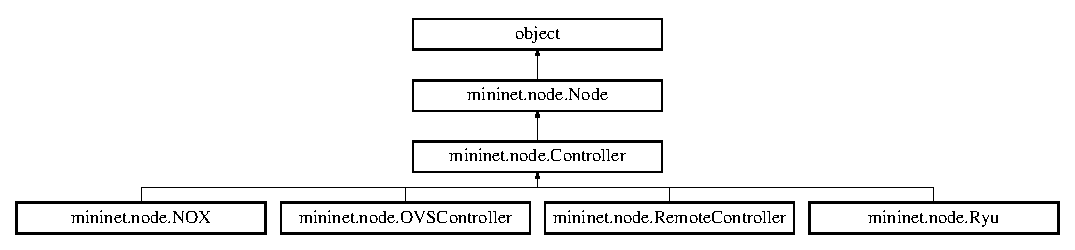
\includegraphics[height=2.916667cm]{classmininet_1_1node_1_1Controller}
\end{center}
\end{figure}
\subsection*{Public Member Functions}
\begin{DoxyCompactItemize}
\item 
\hypertarget{classmininet_1_1node_1_1Controller_a89e3723e45bedf6ad484a4a82ef73f0a}{def {\bfseries \-\_\-\-\_\-init\-\_\-\-\_\-}}\label{classmininet_1_1node_1_1Controller_a89e3723e45bedf6ad484a4a82ef73f0a}

\item 
\hypertarget{classmininet_1_1node_1_1Controller_ad6f82a1a6056b2894042686cf4cef19f}{def {\bfseries check\-Listening}}\label{classmininet_1_1node_1_1Controller_ad6f82a1a6056b2894042686cf4cef19f}

\item 
def \hyperlink{classmininet_1_1node_1_1Controller_a23e3b9dc42d2db34706239a65a997f70}{start}
\item 
\hypertarget{classmininet_1_1node_1_1Controller_ab63d40ad0bceef68ad27872bf95f3adb}{def {\bfseries stop}}\label{classmininet_1_1node_1_1Controller_ab63d40ad0bceef68ad27872bf95f3adb}

\item 
\hypertarget{classmininet_1_1node_1_1Controller_a8f78114d7f0a1d6af19cb84f17a7c273}{def {\bfseries I\-P}}\label{classmininet_1_1node_1_1Controller_a8f78114d7f0a1d6af19cb84f17a7c273}

\item 
\hypertarget{classmininet_1_1node_1_1Controller_aa162bac2708a851038a1e7872211d332}{def {\bfseries \-\_\-\-\_\-repr\-\_\-\-\_\-}}\label{classmininet_1_1node_1_1Controller_aa162bac2708a851038a1e7872211d332}

\item 
\hypertarget{classmininet_1_1node_1_1Controller_aebc0b5c063714b974b3fee15069eecc6}{def {\bfseries is\-Available}}\label{classmininet_1_1node_1_1Controller_aebc0b5c063714b974b3fee15069eecc6}

\end{DoxyCompactItemize}
\subsection*{Public Attributes}
\begin{DoxyCompactItemize}
\item 
\hypertarget{classmininet_1_1node_1_1Controller_ab3b1decf4ea17602e6f64ccce7f5b7ff}{{\bfseries command}}\label{classmininet_1_1node_1_1Controller_ab3b1decf4ea17602e6f64ccce7f5b7ff}

\item 
\hypertarget{classmininet_1_1node_1_1Controller_a5bca25bc759af1a6275870f31d05022a}{{\bfseries cargs}}\label{classmininet_1_1node_1_1Controller_a5bca25bc759af1a6275870f31d05022a}

\item 
\hypertarget{classmininet_1_1node_1_1Controller_a471632985033e1b52232e1550ff8b57e}{{\bfseries cdir}}\label{classmininet_1_1node_1_1Controller_a471632985033e1b52232e1550ff8b57e}

\item 
\hypertarget{classmininet_1_1node_1_1Controller_a8fc2e5696523f9f821fb01904392cdb3}{{\bfseries ip}}\label{classmininet_1_1node_1_1Controller_a8fc2e5696523f9f821fb01904392cdb3}

\item 
\hypertarget{classmininet_1_1node_1_1Controller_acb15ce19a07f469ba457b09f5cdee7f7}{{\bfseries port}}\label{classmininet_1_1node_1_1Controller_acb15ce19a07f469ba457b09f5cdee7f7}

\item 
\hypertarget{classmininet_1_1node_1_1Controller_a2c5d2f00f45148638b1c2f9646bd6d33}{{\bfseries protocol}}\label{classmininet_1_1node_1_1Controller_a2c5d2f00f45148638b1c2f9646bd6d33}

\item 
\hypertarget{classmininet_1_1node_1_1Controller_afca6829cdf74d74ecc9de9a21330efed}{{\bfseries execed}}\label{classmininet_1_1node_1_1Controller_afca6829cdf74d74ecc9de9a21330efed}

\end{DoxyCompactItemize}
\subsection*{Additional Inherited Members}


\subsection{Detailed Description}
\begin{DoxyVerb}A Controller is a Node that is running (or has execed?) an
   OpenFlow controller.\end{DoxyVerb}
 

\subsection{Member Function Documentation}
\hypertarget{classmininet_1_1node_1_1Controller_a23e3b9dc42d2db34706239a65a997f70}{\index{mininet\-::node\-::\-Controller@{mininet\-::node\-::\-Controller}!start@{start}}
\index{start@{start}!mininet::node::Controller@{mininet\-::node\-::\-Controller}}
\subsubsection[{start}]{\setlength{\rightskip}{0pt plus 5cm}def mininet.\-node.\-Controller.\-start (
\begin{DoxyParamCaption}
\item[{}]{self}
\end{DoxyParamCaption}
)}}\label{classmininet_1_1node_1_1Controller_a23e3b9dc42d2db34706239a65a997f70}
\begin{DoxyVerb}Start <controller> <args> on controller.
   Log to /tmp/cN.log\end{DoxyVerb}
 

The documentation for this class was generated from the following file\-:\begin{DoxyCompactItemize}
\item 
node.\-py\end{DoxyCompactItemize}

\hypertarget{classmininet_1_1node_1_1CPULimitedHost}{\section{mininet.\-node.\-C\-P\-U\-Limited\-Host Class Reference}
\label{classmininet_1_1node_1_1CPULimitedHost}\index{mininet.\-node.\-C\-P\-U\-Limited\-Host@{mininet.\-node.\-C\-P\-U\-Limited\-Host}}
}
Inheritance diagram for mininet.\-node.\-C\-P\-U\-Limited\-Host\-:\begin{figure}[H]
\begin{center}
\leavevmode
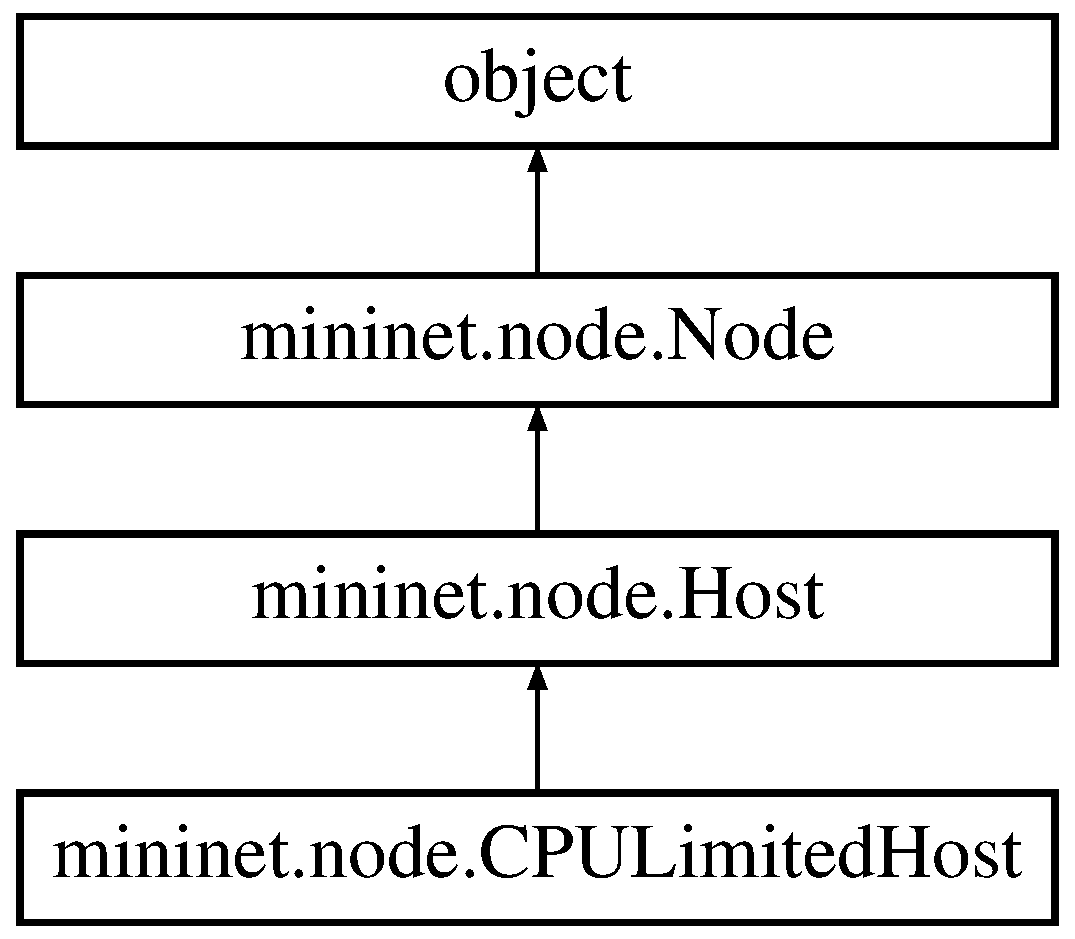
\includegraphics[height=4.000000cm]{classmininet_1_1node_1_1CPULimitedHost}
\end{center}
\end{figure}
\subsection*{Public Member Functions}
\begin{DoxyCompactItemize}
\item 
\hypertarget{classmininet_1_1node_1_1CPULimitedHost_ab553e99e9e6da980ae1db824bd47179a}{def {\bfseries \-\_\-\-\_\-init\-\_\-\-\_\-}}\label{classmininet_1_1node_1_1CPULimitedHost_ab553e99e9e6da980ae1db824bd47179a}

\item 
\hypertarget{classmininet_1_1node_1_1CPULimitedHost_a1b0abcf1dcf7ca1f6da3bfe0dbb483c7}{def {\bfseries cgroup\-Set}}\label{classmininet_1_1node_1_1CPULimitedHost_a1b0abcf1dcf7ca1f6da3bfe0dbb483c7}

\item 
\hypertarget{classmininet_1_1node_1_1CPULimitedHost_a3e88b301839d4c5e0c806e90d1994f24}{def {\bfseries cgroup\-Get}}\label{classmininet_1_1node_1_1CPULimitedHost_a3e88b301839d4c5e0c806e90d1994f24}

\item 
\hypertarget{classmininet_1_1node_1_1CPULimitedHost_ab53c71fa355049c37610e2bdfb3e3388}{def {\bfseries cgroup\-Del}}\label{classmininet_1_1node_1_1CPULimitedHost_ab53c71fa355049c37610e2bdfb3e3388}

\item 
def \hyperlink{classmininet_1_1node_1_1CPULimitedHost_af08d9d9f59e6c1200415ad59f502b170}{popen}
\item 
\hypertarget{classmininet_1_1node_1_1CPULimitedHost_a29fa8f056991ad3f6dff550b2950c3eb}{def {\bfseries cleanup}}\label{classmininet_1_1node_1_1CPULimitedHost_a29fa8f056991ad3f6dff550b2950c3eb}

\item 
\hypertarget{classmininet_1_1node_1_1CPULimitedHost_ac712eaf0a7c30885b1cae4f6b4e26dcc}{def {\bfseries check\-Rt\-Group\-Sched}}\label{classmininet_1_1node_1_1CPULimitedHost_ac712eaf0a7c30885b1cae4f6b4e26dcc}

\item 
\hypertarget{classmininet_1_1node_1_1CPULimitedHost_a84d29a15de4a29ef0a1476d063b0922e}{def {\bfseries chrt}}\label{classmininet_1_1node_1_1CPULimitedHost_a84d29a15de4a29ef0a1476d063b0922e}

\item 
\hypertarget{classmininet_1_1node_1_1CPULimitedHost_aa2c2d839296d4263d43cdef01a65e824}{def {\bfseries rt\-Info}}\label{classmininet_1_1node_1_1CPULimitedHost_aa2c2d839296d4263d43cdef01a65e824}

\item 
\hypertarget{classmininet_1_1node_1_1CPULimitedHost_acf245583d8b0891a12c23ec3b97ffc3d}{def {\bfseries cfs\-Info}}\label{classmininet_1_1node_1_1CPULimitedHost_acf245583d8b0891a12c23ec3b97ffc3d}

\item 
def \hyperlink{classmininet_1_1node_1_1CPULimitedHost_a64f4850bc132e00169b8bb4781d2f21b}{set\-C\-P\-U\-Frac}
\item 
\hypertarget{classmininet_1_1node_1_1CPULimitedHost_ae5ee608818338a0d19a9b348c94c27fa}{def {\bfseries set\-C\-P\-Us}}\label{classmininet_1_1node_1_1CPULimitedHost_ae5ee608818338a0d19a9b348c94c27fa}

\item 
def \hyperlink{classmininet_1_1node_1_1CPULimitedHost_a7b29d14c39b0e64299f8e81e91892440}{config}
\item 
\hypertarget{classmininet_1_1node_1_1CPULimitedHost_a18d3f5c20a6ddf67a1af88b18793a894}{def {\bfseries init}}\label{classmininet_1_1node_1_1CPULimitedHost_a18d3f5c20a6ddf67a1af88b18793a894}

\end{DoxyCompactItemize}
\subsection*{Public Attributes}
\begin{DoxyCompactItemize}
\item 
\hypertarget{classmininet_1_1node_1_1CPULimitedHost_af76af0b4463243d349c28fc099846110}{{\bfseries cgroup}}\label{classmininet_1_1node_1_1CPULimitedHost_af76af0b4463243d349c28fc099846110}

\item 
\hypertarget{classmininet_1_1node_1_1CPULimitedHost_adfb90735daa9502a5193b927db207bab}{{\bfseries period\-\_\-us}}\label{classmininet_1_1node_1_1CPULimitedHost_adfb90735daa9502a5193b927db207bab}

\item 
\hypertarget{classmininet_1_1node_1_1CPULimitedHost_a35ed92fadd20a9dfc3883e305cdf7ba1}{{\bfseries sched}}\label{classmininet_1_1node_1_1CPULimitedHost_a35ed92fadd20a9dfc3883e305cdf7ba1}

\item 
\hypertarget{classmininet_1_1node_1_1CPULimitedHost_aceba3041bb882c4cb1bac69eca00661c}{{\bfseries rtprio}}\label{classmininet_1_1node_1_1CPULimitedHost_aceba3041bb882c4cb1bac69eca00661c}

\end{DoxyCompactItemize}
\subsection*{Static Public Attributes}
\begin{DoxyCompactItemize}
\item 
\hypertarget{classmininet_1_1node_1_1CPULimitedHost_af75961fdf5ac3f8e5419eeb5ab98e489}{{\bfseries inited} = False}\label{classmininet_1_1node_1_1CPULimitedHost_af75961fdf5ac3f8e5419eeb5ab98e489}

\end{DoxyCompactItemize}


\subsection{Member Function Documentation}
\hypertarget{classmininet_1_1node_1_1CPULimitedHost_a7b29d14c39b0e64299f8e81e91892440}{\index{mininet\-::node\-::\-C\-P\-U\-Limited\-Host@{mininet\-::node\-::\-C\-P\-U\-Limited\-Host}!config@{config}}
\index{config@{config}!mininet::node::CPULimitedHost@{mininet\-::node\-::\-C\-P\-U\-Limited\-Host}}
\subsubsection[{config}]{\setlength{\rightskip}{0pt plus 5cm}def mininet.\-node.\-C\-P\-U\-Limited\-Host.\-config (
\begin{DoxyParamCaption}
\item[{}]{self, }
\item[{}]{cpu = {\ttfamily -\/1}, }
\item[{}]{cores = {\ttfamily None}, }
\item[{}]{params}
\end{DoxyParamCaption}
)}}\label{classmininet_1_1node_1_1CPULimitedHost_a7b29d14c39b0e64299f8e81e91892440}
\begin{DoxyVerb}cpu: desired overall system CPU fraction
   cores: (real) core(s) this host can run on
   params: parameters for Node.config()\end{DoxyVerb}
 \hypertarget{classmininet_1_1node_1_1CPULimitedHost_af08d9d9f59e6c1200415ad59f502b170}{\index{mininet\-::node\-::\-C\-P\-U\-Limited\-Host@{mininet\-::node\-::\-C\-P\-U\-Limited\-Host}!popen@{popen}}
\index{popen@{popen}!mininet::node::CPULimitedHost@{mininet\-::node\-::\-C\-P\-U\-Limited\-Host}}
\subsubsection[{popen}]{\setlength{\rightskip}{0pt plus 5cm}def mininet.\-node.\-C\-P\-U\-Limited\-Host.\-popen (
\begin{DoxyParamCaption}
\item[{}]{self, }
\item[{}]{args, }
\item[{}]{kwargs}
\end{DoxyParamCaption}
)}}\label{classmininet_1_1node_1_1CPULimitedHost_af08d9d9f59e6c1200415ad59f502b170}
\begin{DoxyVerb}Return a Popen() object in node's namespace
   args: Popen() args, single list, or string
   kwargs: Popen() keyword args\end{DoxyVerb}
 \hypertarget{classmininet_1_1node_1_1CPULimitedHost_a64f4850bc132e00169b8bb4781d2f21b}{\index{mininet\-::node\-::\-C\-P\-U\-Limited\-Host@{mininet\-::node\-::\-C\-P\-U\-Limited\-Host}!set\-C\-P\-U\-Frac@{set\-C\-P\-U\-Frac}}
\index{set\-C\-P\-U\-Frac@{set\-C\-P\-U\-Frac}!mininet::node::CPULimitedHost@{mininet\-::node\-::\-C\-P\-U\-Limited\-Host}}
\subsubsection[{set\-C\-P\-U\-Frac}]{\setlength{\rightskip}{0pt plus 5cm}def mininet.\-node.\-C\-P\-U\-Limited\-Host.\-set\-C\-P\-U\-Frac (
\begin{DoxyParamCaption}
\item[{}]{self, }
\item[{}]{f, }
\item[{}]{sched = {\ttfamily None}}
\end{DoxyParamCaption}
)}}\label{classmininet_1_1node_1_1CPULimitedHost_a64f4850bc132e00169b8bb4781d2f21b}
\begin{DoxyVerb}Set overall CPU fraction for this host
   f: CPU bandwidth limit (positive fraction, or -1 for cfs unlimited)
   sched: 'rt' or 'cfs'
   Note 'cfs' requires CONFIG_CFS_BANDWIDTH,
   and 'rt' requires CONFIG_RT_GROUP_SCHED\end{DoxyVerb}
 

The documentation for this class was generated from the following file\-:\begin{DoxyCompactItemize}
\item 
node.\-py\end{DoxyCompactItemize}

\hypertarget{classmininet_1_1wifiDevices_1_1deviceDataRate}{\section{mininet.\-wifi\-Devices.\-device\-Data\-Rate Class Reference}
\label{classmininet_1_1wifiDevices_1_1deviceDataRate}\index{mininet.\-wifi\-Devices.\-device\-Data\-Rate@{mininet.\-wifi\-Devices.\-device\-Data\-Rate}}
}
Inheritance diagram for mininet.\-wifi\-Devices.\-device\-Data\-Rate\-:\begin{figure}[H]
\begin{center}
\leavevmode
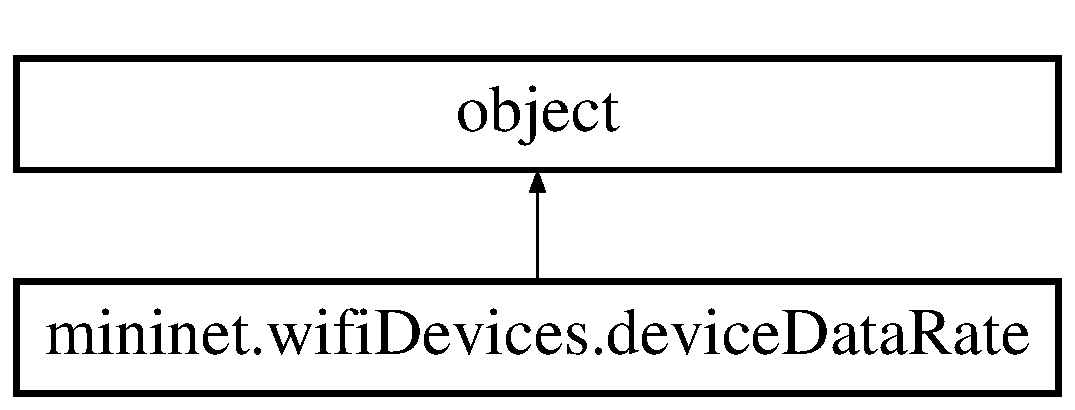
\includegraphics[height=2.000000cm]{classmininet_1_1wifiDevices_1_1deviceDataRate}
\end{center}
\end{figure}
\subsection*{Public Member Functions}
\begin{DoxyCompactItemize}
\item 
\hypertarget{classmininet_1_1wifiDevices_1_1deviceDataRate_a4fec299443675f5f03329b2265f13f5d}{def {\bfseries \-\_\-\-\_\-init\-\_\-\-\_\-}}\label{classmininet_1_1wifiDevices_1_1deviceDataRate_a4fec299443675f5f03329b2265f13f5d}

\item 
def \hyperlink{classmininet_1_1wifiDevices_1_1deviceDataRate_a90f2be44dbbb1551f568b80dc0d002f8}{custom\-Data\-Rate\-\_\-mobility}
\item 
def \hyperlink{classmininet_1_1wifiDevices_1_1deviceDataRate_ab29cfdb142580593f09f4c8b112a5512}{custom\-Data\-Rate\-\_\-no\-\_\-mobility}
\item 
def \hyperlink{classmininet_1_1wifiDevices_1_1deviceDataRate_ab2be9df8a52b025219584371b39fadf7}{D\-I524}
\item 
def \hyperlink{classmininet_1_1wifiDevices_1_1deviceDataRate_a79fa9b37c33e24e8fc8ffd6c2cb45a98}{T\-L\-W\-R740\-N}
\item 
def \hyperlink{classmininet_1_1wifiDevices_1_1deviceDataRate_a97ca6b84adfb0cb4f02d826219cdab80}{W\-R\-T120\-N}
\end{DoxyCompactItemize}
\subsection*{Public Attributes}
\begin{DoxyCompactItemize}
\item 
\hypertarget{classmininet_1_1wifiDevices_1_1deviceDataRate_ac0c77c60bdc09f6cc259794e10662ffd}{{\bfseries rate}}\label{classmininet_1_1wifiDevices_1_1deviceDataRate_ac0c77c60bdc09f6cc259794e10662ffd}

\end{DoxyCompactItemize}
\subsection*{Static Public Attributes}
\begin{DoxyCompactItemize}
\item 
\hypertarget{classmininet_1_1wifiDevices_1_1deviceDataRate_a842f913dc88098b3c8c8b0b0120b9df2}{int {\bfseries rate} = 0}\label{classmininet_1_1wifiDevices_1_1deviceDataRate_a842f913dc88098b3c8c8b0b0120b9df2}

\end{DoxyCompactItemize}


\subsection{Detailed Description}
\begin{DoxyVerb}Data Rate for specific equipments \end{DoxyVerb}
 

\subsection{Member Function Documentation}
\hypertarget{classmininet_1_1wifiDevices_1_1deviceDataRate_a90f2be44dbbb1551f568b80dc0d002f8}{\index{mininet\-::wifi\-Devices\-::device\-Data\-Rate@{mininet\-::wifi\-Devices\-::device\-Data\-Rate}!custom\-Data\-Rate\-\_\-mobility@{custom\-Data\-Rate\-\_\-mobility}}
\index{custom\-Data\-Rate\-\_\-mobility@{custom\-Data\-Rate\-\_\-mobility}!mininet::wifiDevices::deviceDataRate@{mininet\-::wifi\-Devices\-::device\-Data\-Rate}}
\subsubsection[{custom\-Data\-Rate\-\_\-mobility}]{\setlength{\rightskip}{0pt plus 5cm}def mininet.\-wifi\-Devices.\-device\-Data\-Rate.\-custom\-Data\-Rate\-\_\-mobility (
\begin{DoxyParamCaption}
\item[{}]{self, }
\item[{}]{node}
\end{DoxyParamCaption}
)}}\label{classmininet_1_1wifiDevices_1_1deviceDataRate_a90f2be44dbbb1551f568b80dc0d002f8}
\begin{DoxyVerb}Custom Maximum Data Rate - Useful when there is mobility\end{DoxyVerb}
 \hypertarget{classmininet_1_1wifiDevices_1_1deviceDataRate_ab29cfdb142580593f09f4c8b112a5512}{\index{mininet\-::wifi\-Devices\-::device\-Data\-Rate@{mininet\-::wifi\-Devices\-::device\-Data\-Rate}!custom\-Data\-Rate\-\_\-no\-\_\-mobility@{custom\-Data\-Rate\-\_\-no\-\_\-mobility}}
\index{custom\-Data\-Rate\-\_\-no\-\_\-mobility@{custom\-Data\-Rate\-\_\-no\-\_\-mobility}!mininet::wifiDevices::deviceDataRate@{mininet\-::wifi\-Devices\-::device\-Data\-Rate}}
\subsubsection[{custom\-Data\-Rate\-\_\-no\-\_\-mobility}]{\setlength{\rightskip}{0pt plus 5cm}def mininet.\-wifi\-Devices.\-device\-Data\-Rate.\-custom\-Data\-Rate\-\_\-no\-\_\-mobility (
\begin{DoxyParamCaption}
\item[{}]{self, }
\item[{}]{node}
\end{DoxyParamCaption}
)}}\label{classmininet_1_1wifiDevices_1_1deviceDataRate_ab29cfdb142580593f09f4c8b112a5512}
\begin{DoxyVerb}Custom Maximum Data Rate - Useful when there is no mobility\end{DoxyVerb}
 \hypertarget{classmininet_1_1wifiDevices_1_1deviceDataRate_ab2be9df8a52b025219584371b39fadf7}{\index{mininet\-::wifi\-Devices\-::device\-Data\-Rate@{mininet\-::wifi\-Devices\-::device\-Data\-Rate}!D\-I524@{D\-I524}}
\index{D\-I524@{D\-I524}!mininet::wifiDevices::deviceDataRate@{mininet\-::wifi\-Devices\-::device\-Data\-Rate}}
\subsubsection[{D\-I524}]{\setlength{\rightskip}{0pt plus 5cm}def mininet.\-wifi\-Devices.\-device\-Data\-Rate.\-D\-I524 (
\begin{DoxyParamCaption}
\item[{}]{self, }
\item[{}]{node1, }
\item[{}]{node2, }
\item[{}]{wlan}
\end{DoxyParamCaption}
)}}\label{classmininet_1_1wifiDevices_1_1deviceDataRate_ab2be9df8a52b025219584371b39fadf7}
\begin{DoxyVerb}D-Link AirPlus G DI-524
   from http://www.dlink.com/-/media/Consumer_Products/DI/DI%20524/Manual/DI_524_Manual_EN_UK.pdf\end{DoxyVerb}
 \hypertarget{classmininet_1_1wifiDevices_1_1deviceDataRate_a79fa9b37c33e24e8fc8ffd6c2cb45a98}{\index{mininet\-::wifi\-Devices\-::device\-Data\-Rate@{mininet\-::wifi\-Devices\-::device\-Data\-Rate}!T\-L\-W\-R740\-N@{T\-L\-W\-R740\-N}}
\index{T\-L\-W\-R740\-N@{T\-L\-W\-R740\-N}!mininet::wifiDevices::deviceDataRate@{mininet\-::wifi\-Devices\-::device\-Data\-Rate}}
\subsubsection[{T\-L\-W\-R740\-N}]{\setlength{\rightskip}{0pt plus 5cm}def mininet.\-wifi\-Devices.\-device\-Data\-Rate.\-T\-L\-W\-R740\-N (
\begin{DoxyParamCaption}
\item[{}]{self, }
\item[{}]{node1, }
\item[{}]{node2, }
\item[{}]{wlan}
\end{DoxyParamCaption}
)}}\label{classmininet_1_1wifiDevices_1_1deviceDataRate_a79fa9b37c33e24e8fc8ffd6c2cb45a98}
\begin{DoxyVerb}TL-WR740N
   from http://www.tp-link.com.br/products/details/cat-9_TL-WR740N.html#specificationsf\end{DoxyVerb}
 \hypertarget{classmininet_1_1wifiDevices_1_1deviceDataRate_a97ca6b84adfb0cb4f02d826219cdab80}{\index{mininet\-::wifi\-Devices\-::device\-Data\-Rate@{mininet\-::wifi\-Devices\-::device\-Data\-Rate}!W\-R\-T120\-N@{W\-R\-T120\-N}}
\index{W\-R\-T120\-N@{W\-R\-T120\-N}!mininet::wifiDevices::deviceDataRate@{mininet\-::wifi\-Devices\-::device\-Data\-Rate}}
\subsubsection[{W\-R\-T120\-N}]{\setlength{\rightskip}{0pt plus 5cm}def mininet.\-wifi\-Devices.\-device\-Data\-Rate.\-W\-R\-T120\-N (
\begin{DoxyParamCaption}
\item[{}]{self, }
\item[{}]{node1, }
\item[{}]{node2, }
\item[{}]{wlan}
\end{DoxyParamCaption}
)}}\label{classmininet_1_1wifiDevices_1_1deviceDataRate_a97ca6b84adfb0cb4f02d826219cdab80}
\begin{DoxyVerb}CISCO WRT120N
   from http://downloads.linksys.com/downloads/datasheet/WRT120N_V10_DS_B-WEB.pdf\end{DoxyVerb}
 

The documentation for this class was generated from the following file\-:\begin{DoxyCompactItemize}
\item 
wifi\-Devices.\-py\end{DoxyCompactItemize}

\hypertarget{classmininet_1_1wifiDevices_1_1deviceRange}{\section{mininet.\-wifi\-Devices.\-device\-Range Class Reference}
\label{classmininet_1_1wifiDevices_1_1deviceRange}\index{mininet.\-wifi\-Devices.\-device\-Range@{mininet.\-wifi\-Devices.\-device\-Range}}
}
Inheritance diagram for mininet.\-wifi\-Devices.\-device\-Range\-:\begin{figure}[H]
\begin{center}
\leavevmode
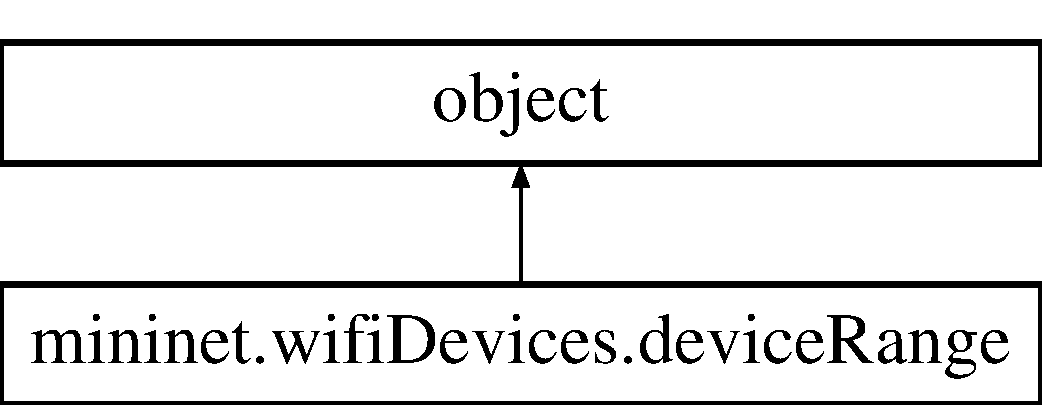
\includegraphics[height=2.000000cm]{classmininet_1_1wifiDevices_1_1deviceRange}
\end{center}
\end{figure}
\subsection*{Public Member Functions}
\begin{DoxyCompactItemize}
\item 
\hypertarget{classmininet_1_1wifiDevices_1_1deviceRange_ad7fe42f9f0a307c3444db23c944332f2}{def {\bfseries \-\_\-\-\_\-init\-\_\-\-\_\-}}\label{classmininet_1_1wifiDevices_1_1deviceRange_ad7fe42f9f0a307c3444db23c944332f2}

\item 
def \hyperlink{classmininet_1_1wifiDevices_1_1deviceRange_a388df9e7ba2079a449f3d9b2747849f2}{custom\-Signal\-Range}
\item 
def \hyperlink{classmininet_1_1wifiDevices_1_1deviceRange_a2919231acd6495a7614656ef3ef8a085}{D\-I524}
\item 
def \hyperlink{classmininet_1_1wifiDevices_1_1deviceRange_aa6d5de3aa8cd6a716e765055275d8825}{T\-L\-W\-R740\-N}
\item 
def \hyperlink{classmininet_1_1wifiDevices_1_1deviceRange_a883ce479154210f8857eb32592f2ad96}{W\-R\-T120\-N}
\end{DoxyCompactItemize}
\subsection*{Public Attributes}
\begin{DoxyCompactItemize}
\item 
\hypertarget{classmininet_1_1wifiDevices_1_1deviceRange_ab7caf7221bd5cb4ca0cab747a68d85a7}{{\bfseries equipment\-Model}}\label{classmininet_1_1wifiDevices_1_1deviceRange_ab7caf7221bd5cb4ca0cab747a68d85a7}

\item 
\hypertarget{classmininet_1_1wifiDevices_1_1deviceRange_a341daacf0384625393be41b701980325}{{\bfseries node}}\label{classmininet_1_1wifiDevices_1_1deviceRange_a341daacf0384625393be41b701980325}

\item 
\hypertarget{classmininet_1_1wifiDevices_1_1deviceRange_a43f07302f4cc265a635475d9ba8e6a2c}{{\bfseries range}}\label{classmininet_1_1wifiDevices_1_1deviceRange_a43f07302f4cc265a635475d9ba8e6a2c}

\end{DoxyCompactItemize}
\subsection*{Static Public Attributes}
\begin{DoxyCompactItemize}
\item 
\hypertarget{classmininet_1_1wifiDevices_1_1deviceRange_a755e774fe66ffe18f7838ac107531f2a}{int {\bfseries range} = 100}\label{classmininet_1_1wifiDevices_1_1deviceRange_a755e774fe66ffe18f7838ac107531f2a}

\end{DoxyCompactItemize}


\subsection{Detailed Description}
\begin{DoxyVerb}Range for specific equipments \end{DoxyVerb}
 

\subsection{Member Function Documentation}
\hypertarget{classmininet_1_1wifiDevices_1_1deviceRange_a388df9e7ba2079a449f3d9b2747849f2}{\index{mininet\-::wifi\-Devices\-::device\-Range@{mininet\-::wifi\-Devices\-::device\-Range}!custom\-Signal\-Range@{custom\-Signal\-Range}}
\index{custom\-Signal\-Range@{custom\-Signal\-Range}!mininet::wifiDevices::deviceRange@{mininet\-::wifi\-Devices\-::device\-Range}}
\subsubsection[{custom\-Signal\-Range}]{\setlength{\rightskip}{0pt plus 5cm}def mininet.\-wifi\-Devices.\-device\-Range.\-custom\-Signal\-Range (
\begin{DoxyParamCaption}
\item[{}]{self, }
\item[{}]{node}
\end{DoxyParamCaption}
)}}\label{classmininet_1_1wifiDevices_1_1deviceRange_a388df9e7ba2079a449f3d9b2747849f2}
\begin{DoxyVerb}Custom Signal Range\end{DoxyVerb}
 \hypertarget{classmininet_1_1wifiDevices_1_1deviceRange_a2919231acd6495a7614656ef3ef8a085}{\index{mininet\-::wifi\-Devices\-::device\-Range@{mininet\-::wifi\-Devices\-::device\-Range}!D\-I524@{D\-I524}}
\index{D\-I524@{D\-I524}!mininet::wifiDevices::deviceRange@{mininet\-::wifi\-Devices\-::device\-Range}}
\subsubsection[{D\-I524}]{\setlength{\rightskip}{0pt plus 5cm}def mininet.\-wifi\-Devices.\-device\-Range.\-D\-I524 (
\begin{DoxyParamCaption}
\item[{}]{self, }
\item[{}]{ap}
\end{DoxyParamCaption}
)}}\label{classmininet_1_1wifiDevices_1_1deviceRange_a2919231acd6495a7614656ef3ef8a085}
\begin{DoxyVerb}D-Link AirPlus G DI-524
    from http://www.dlink.com/-/media/Consumer_Products/DI/DI%20524/Manual/DI_524_Manual_EN_UK.pdf
    indoor = 100
    outdoor = 200 \end{DoxyVerb}
 \hypertarget{classmininet_1_1wifiDevices_1_1deviceRange_aa6d5de3aa8cd6a716e765055275d8825}{\index{mininet\-::wifi\-Devices\-::device\-Range@{mininet\-::wifi\-Devices\-::device\-Range}!T\-L\-W\-R740\-N@{T\-L\-W\-R740\-N}}
\index{T\-L\-W\-R740\-N@{T\-L\-W\-R740\-N}!mininet::wifiDevices::deviceRange@{mininet\-::wifi\-Devices\-::device\-Range}}
\subsubsection[{T\-L\-W\-R740\-N}]{\setlength{\rightskip}{0pt plus 5cm}def mininet.\-wifi\-Devices.\-device\-Range.\-T\-L\-W\-R740\-N (
\begin{DoxyParamCaption}
\item[{}]{self, }
\item[{}]{ap}
\end{DoxyParamCaption}
)}}\label{classmininet_1_1wifiDevices_1_1deviceRange_aa6d5de3aa8cd6a716e765055275d8825}
\begin{DoxyVerb}TL-WR740N
NO REFERENCE!\end{DoxyVerb}
 \hypertarget{classmininet_1_1wifiDevices_1_1deviceRange_a883ce479154210f8857eb32592f2ad96}{\index{mininet\-::wifi\-Devices\-::device\-Range@{mininet\-::wifi\-Devices\-::device\-Range}!W\-R\-T120\-N@{W\-R\-T120\-N}}
\index{W\-R\-T120\-N@{W\-R\-T120\-N}!mininet::wifiDevices::deviceRange@{mininet\-::wifi\-Devices\-::device\-Range}}
\subsubsection[{W\-R\-T120\-N}]{\setlength{\rightskip}{0pt plus 5cm}def mininet.\-wifi\-Devices.\-device\-Range.\-W\-R\-T120\-N (
\begin{DoxyParamCaption}
\item[{}]{self, }
\item[{}]{ap}
\end{DoxyParamCaption}
)}}\label{classmininet_1_1wifiDevices_1_1deviceRange_a883ce479154210f8857eb32592f2ad96}
\begin{DoxyVerb}CISCO WRT120N
NO REFERENCE!\end{DoxyVerb}
 

The documentation for this class was generated from the following file\-:\begin{DoxyCompactItemize}
\item 
wifi\-Devices.\-py\end{DoxyCompactItemize}

\hypertarget{classmininet_1_1wifiDevices_1_1deviceTxPower}{\section{mininet.\-wifi\-Devices.\-device\-Tx\-Power Class Reference}
\label{classmininet_1_1wifiDevices_1_1deviceTxPower}\index{mininet.\-wifi\-Devices.\-device\-Tx\-Power@{mininet.\-wifi\-Devices.\-device\-Tx\-Power}}
}
Inheritance diagram for mininet.\-wifi\-Devices.\-device\-Tx\-Power\-:\begin{figure}[H]
\begin{center}
\leavevmode
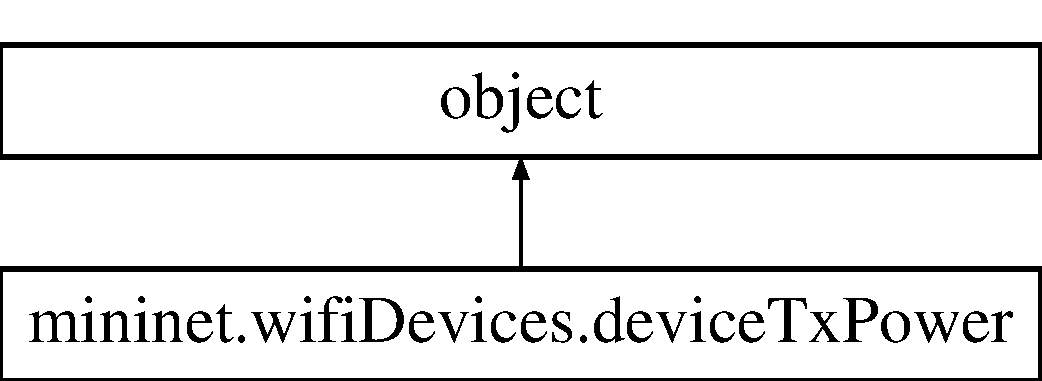
\includegraphics[height=2.000000cm]{classmininet_1_1wifiDevices_1_1deviceTxPower}
\end{center}
\end{figure}
\subsection*{Public Member Functions}
\begin{DoxyCompactItemize}
\item 
\hypertarget{classmininet_1_1wifiDevices_1_1deviceTxPower_a158221f123f7c7fa896ec98d5ef96156}{def {\bfseries \-\_\-\-\_\-init\-\_\-\-\_\-}}\label{classmininet_1_1wifiDevices_1_1deviceTxPower_a158221f123f7c7fa896ec98d5ef96156}

\item 
def \hyperlink{classmininet_1_1wifiDevices_1_1deviceTxPower_a923dbc3d5f6285872a5585b9bbb9603e}{D\-I524}
\item 
def \hyperlink{classmininet_1_1wifiDevices_1_1deviceTxPower_abefb1b3e723b0b13a7c32bd6bfa6fb42}{T\-L\-W\-R740\-N}
\item 
def \hyperlink{classmininet_1_1wifiDevices_1_1deviceTxPower_a33e3e8d506a790dcabac4d2bf2f6aa41}{W\-R\-T120\-N}
\end{DoxyCompactItemize}
\subsection*{Public Attributes}
\begin{DoxyCompactItemize}
\item 
\hypertarget{classmininet_1_1wifiDevices_1_1deviceTxPower_a3096d329e255f5b1bce363bb96a9103b}{{\bfseries model}}\label{classmininet_1_1wifiDevices_1_1deviceTxPower_a3096d329e255f5b1bce363bb96a9103b}

\item 
\hypertarget{classmininet_1_1wifiDevices_1_1deviceTxPower_a598b80138c60920fe32e25198c87ca5a}{{\bfseries ap}}\label{classmininet_1_1wifiDevices_1_1deviceTxPower_a598b80138c60920fe32e25198c87ca5a}

\item 
\hypertarget{classmininet_1_1wifiDevices_1_1deviceTxPower_a3ca46b384fc075c3e8d97eaba7eedf6e}{{\bfseries tx\-Power}}\label{classmininet_1_1wifiDevices_1_1deviceTxPower_a3ca46b384fc075c3e8d97eaba7eedf6e}

\end{DoxyCompactItemize}
\subsection*{Static Public Attributes}
\begin{DoxyCompactItemize}
\item 
\hypertarget{classmininet_1_1wifiDevices_1_1deviceTxPower_a9469bf2bc36993762b237fc8bb76bc59}{int {\bfseries tx\-Power} = 0}\label{classmininet_1_1wifiDevices_1_1deviceTxPower_a9469bf2bc36993762b237fc8bb76bc59}

\end{DoxyCompactItemize}


\subsection{Detailed Description}
\begin{DoxyVerb}TX Power for specific equipments \end{DoxyVerb}
 

\subsection{Member Function Documentation}
\hypertarget{classmininet_1_1wifiDevices_1_1deviceTxPower_a923dbc3d5f6285872a5585b9bbb9603e}{\index{mininet\-::wifi\-Devices\-::device\-Tx\-Power@{mininet\-::wifi\-Devices\-::device\-Tx\-Power}!D\-I524@{D\-I524}}
\index{D\-I524@{D\-I524}!mininet::wifiDevices::deviceTxPower@{mininet\-::wifi\-Devices\-::device\-Tx\-Power}}
\subsubsection[{D\-I524}]{\setlength{\rightskip}{0pt plus 5cm}def mininet.\-wifi\-Devices.\-device\-Tx\-Power.\-D\-I524 (
\begin{DoxyParamCaption}
\item[{}]{self, }
\item[{}]{ap}
\end{DoxyParamCaption}
)}}\label{classmininet_1_1wifiDevices_1_1deviceTxPower_a923dbc3d5f6285872a5585b9bbb9603e}
\begin{DoxyVerb}D-Link AirPlus G DI-524
    from http://www.dlink.com/-/media/Consumer_Products/DI/DI%20524/Manual/DI_524_Manual_EN_UK.pdf\end{DoxyVerb}
 \hypertarget{classmininet_1_1wifiDevices_1_1deviceTxPower_abefb1b3e723b0b13a7c32bd6bfa6fb42}{\index{mininet\-::wifi\-Devices\-::device\-Tx\-Power@{mininet\-::wifi\-Devices\-::device\-Tx\-Power}!T\-L\-W\-R740\-N@{T\-L\-W\-R740\-N}}
\index{T\-L\-W\-R740\-N@{T\-L\-W\-R740\-N}!mininet::wifiDevices::deviceTxPower@{mininet\-::wifi\-Devices\-::device\-Tx\-Power}}
\subsubsection[{T\-L\-W\-R740\-N}]{\setlength{\rightskip}{0pt plus 5cm}def mininet.\-wifi\-Devices.\-device\-Tx\-Power.\-T\-L\-W\-R740\-N (
\begin{DoxyParamCaption}
\item[{}]{self, }
\item[{}]{ap}
\end{DoxyParamCaption}
)}}\label{classmininet_1_1wifiDevices_1_1deviceTxPower_abefb1b3e723b0b13a7c32bd6bfa6fb42}
\begin{DoxyVerb}TL-WR740N
No REFERENCE!\end{DoxyVerb}
 \hypertarget{classmininet_1_1wifiDevices_1_1deviceTxPower_a33e3e8d506a790dcabac4d2bf2f6aa41}{\index{mininet\-::wifi\-Devices\-::device\-Tx\-Power@{mininet\-::wifi\-Devices\-::device\-Tx\-Power}!W\-R\-T120\-N@{W\-R\-T120\-N}}
\index{W\-R\-T120\-N@{W\-R\-T120\-N}!mininet::wifiDevices::deviceTxPower@{mininet\-::wifi\-Devices\-::device\-Tx\-Power}}
\subsubsection[{W\-R\-T120\-N}]{\setlength{\rightskip}{0pt plus 5cm}def mininet.\-wifi\-Devices.\-device\-Tx\-Power.\-W\-R\-T120\-N (
\begin{DoxyParamCaption}
\item[{}]{self, }
\item[{}]{ap}
\end{DoxyParamCaption}
)}}\label{classmininet_1_1wifiDevices_1_1deviceTxPower_a33e3e8d506a790dcabac4d2bf2f6aa41}
\begin{DoxyVerb}CISCO WRT120N
   from http://downloads.linksys.com/downloads/datasheet/WRT120N_V10_DS_B-WEB.pdf\end{DoxyVerb}
 

The documentation for this class was generated from the following file\-:\begin{DoxyCompactItemize}
\item 
wifi\-Devices.\-py\end{DoxyCompactItemize}

\hypertarget{classmininet_1_1wifiMobilityModels_1_1HeterogeneousTruncatedLevyWalk}{\section{mininet.\-wifi\-Mobility\-Models.\-Heterogeneous\-Truncated\-Levy\-Walk Class Reference}
\label{classmininet_1_1wifiMobilityModels_1_1HeterogeneousTruncatedLevyWalk}\index{mininet.\-wifi\-Mobility\-Models.\-Heterogeneous\-Truncated\-Levy\-Walk@{mininet.\-wifi\-Mobility\-Models.\-Heterogeneous\-Truncated\-Levy\-Walk}}
}
Inheritance diagram for mininet.\-wifi\-Mobility\-Models.\-Heterogeneous\-Truncated\-Levy\-Walk\-:\begin{figure}[H]
\begin{center}
\leavevmode
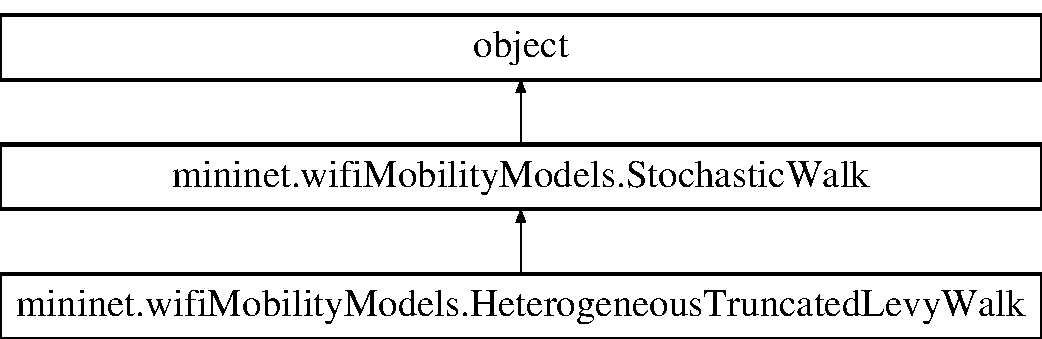
\includegraphics[height=3.000000cm]{classmininet_1_1wifiMobilityModels_1_1HeterogeneousTruncatedLevyWalk}
\end{center}
\end{figure}
\subsection*{Public Member Functions}
\begin{DoxyCompactItemize}
\item 
def \hyperlink{classmininet_1_1wifiMobilityModels_1_1HeterogeneousTruncatedLevyWalk_ac62818e40549480321577341bc96efe4}{\-\_\-\-\_\-init\-\_\-\-\_\-}
\end{DoxyCompactItemize}
\subsection*{Additional Inherited Members}


\subsection{Constructor \& Destructor Documentation}
\hypertarget{classmininet_1_1wifiMobilityModels_1_1HeterogeneousTruncatedLevyWalk_ac62818e40549480321577341bc96efe4}{\index{mininet\-::wifi\-Mobility\-Models\-::\-Heterogeneous\-Truncated\-Levy\-Walk@{mininet\-::wifi\-Mobility\-Models\-::\-Heterogeneous\-Truncated\-Levy\-Walk}!\-\_\-\-\_\-init\-\_\-\-\_\-@{\-\_\-\-\_\-init\-\_\-\-\_\-}}
\index{\-\_\-\-\_\-init\-\_\-\-\_\-@{\-\_\-\-\_\-init\-\_\-\-\_\-}!mininet::wifiMobilityModels::HeterogeneousTruncatedLevyWalk@{mininet\-::wifi\-Mobility\-Models\-::\-Heterogeneous\-Truncated\-Levy\-Walk}}
\subsubsection[{\-\_\-\-\_\-init\-\_\-\-\_\-}]{\setlength{\rightskip}{0pt plus 5cm}def mininet.\-wifi\-Mobility\-Models.\-Heterogeneous\-Truncated\-Levy\-Walk.\-\_\-\-\_\-init\-\_\-\-\_\- (
\begin{DoxyParamCaption}
\item[{}]{self, }
\item[{}]{nr\-\_\-nodes, }
\item[{}]{dimensions, }
\item[{}]{W\-T\-\_\-\-E\-X\-P = {\ttfamily -\/1.8}, }
\item[{}]{W\-T\-\_\-\-M\-A\-X = {\ttfamily 100.}, }
\item[{}]{F\-L\-\_\-\-E\-X\-P = {\ttfamily -\/2.6}, }
\item[{}]{F\-L\-\_\-\-M\-A\-X = {\ttfamily 50.}, }
\item[{}]{border\-\_\-policy = {\ttfamily 'reflect'}}
\end{DoxyParamCaption}
)}}\label{classmininet_1_1wifiMobilityModels_1_1HeterogeneousTruncatedLevyWalk_ac62818e40549480321577341bc96efe4}
\begin{DoxyVerb}This is a variant of the Truncated Levy Walk mobility model.
This model is based in the Stochastic Walk.
The waiting time distribution is a truncated power law with exponent set to WT_EXP and truncated WT_MAX.
The flight length is a uniform distribution, different for each node. These uniform distributions are 
created by taking both min and max values from a power law with exponent set to FL_EXP and truncated FL_MAX.
The node velocity is a function of the flight length.

Required arguments:

  *nr_nodes*:
    Integer, the number of nodes.
  
  *dimensions*:
    Tuple of Integers, the x and y dimensions of the simulation area.
  
keyword arguments:

  *WT_EXP*:
    Double, the exponent of the waiting time distribution. Default is -1.8
    
  *WT_MAX*:
    Double, the maximum value of the waiting time distribution. Default is 100

  *FL_EXP*:
    Double, the exponent of the flight length distribution. Default is -2.6
    
  *FL_MAX*:
    Double, the maximum value of the flight length distribution. Default is 50
    
  *border_policy*:
    String, either 'reflect' or 'wrap'. The policy that is used when the node arrives to the border.
    If 'reflect', the node reflects off the border.
    If 'wrap', the node reappears at the opposite edge (as in a torus-shaped area).
\end{DoxyVerb}
 

The documentation for this class was generated from the following file\-:\begin{DoxyCompactItemize}
\item 
wifi\-Mobility\-Models.\-py\end{DoxyCompactItemize}

\hypertarget{classmininet_1_1node_1_1Host}{\section{mininet.\-node.\-Host Class Reference}
\label{classmininet_1_1node_1_1Host}\index{mininet.\-node.\-Host@{mininet.\-node.\-Host}}
}
Inheritance diagram for mininet.\-node.\-Host\-:\begin{figure}[H]
\begin{center}
\leavevmode
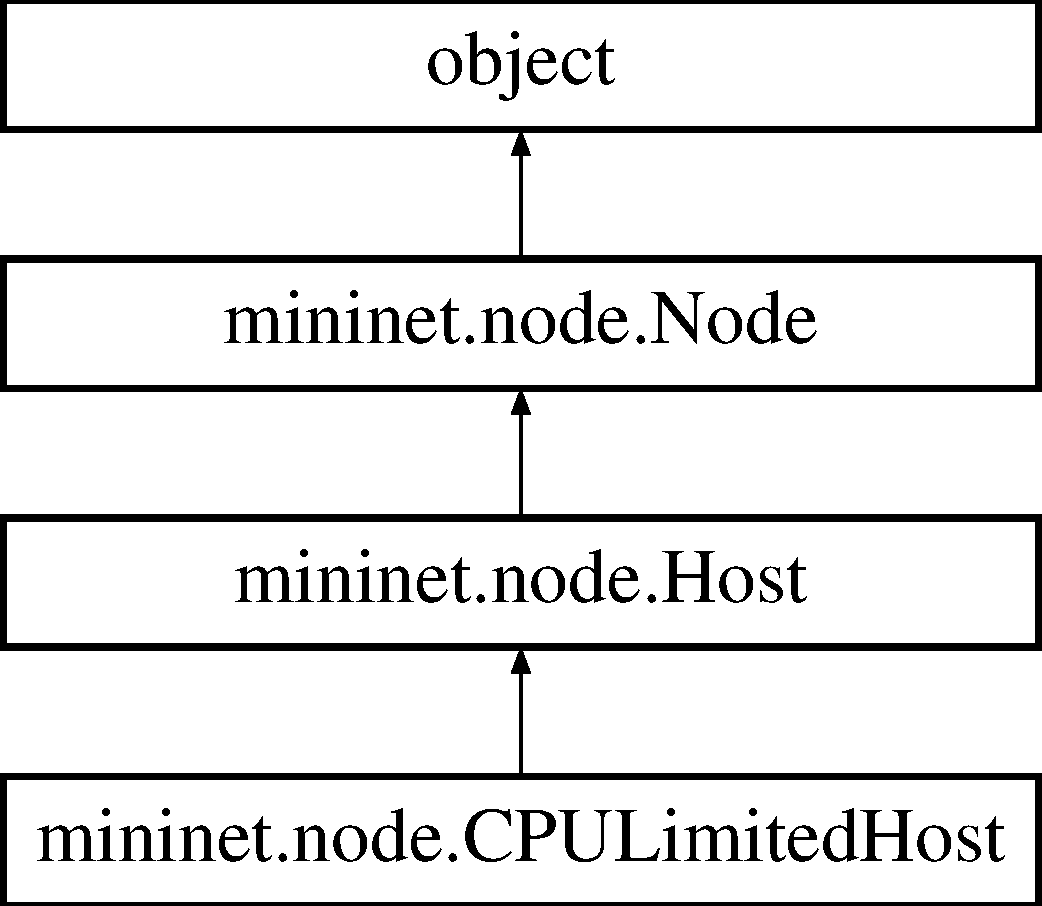
\includegraphics[height=4.000000cm]{classmininet_1_1node_1_1Host}
\end{center}
\end{figure}
\subsection*{Additional Inherited Members}


The documentation for this class was generated from the following file\-:\begin{DoxyCompactItemize}
\item 
node.\-py\end{DoxyCompactItemize}

\hypertarget{classmininet_1_1link_1_1Intf}{\section{mininet.\-link.\-Intf Class Reference}
\label{classmininet_1_1link_1_1Intf}\index{mininet.\-link.\-Intf@{mininet.\-link.\-Intf}}
}
Inheritance diagram for mininet.\-link.\-Intf\-:\begin{figure}[H]
\begin{center}
\leavevmode
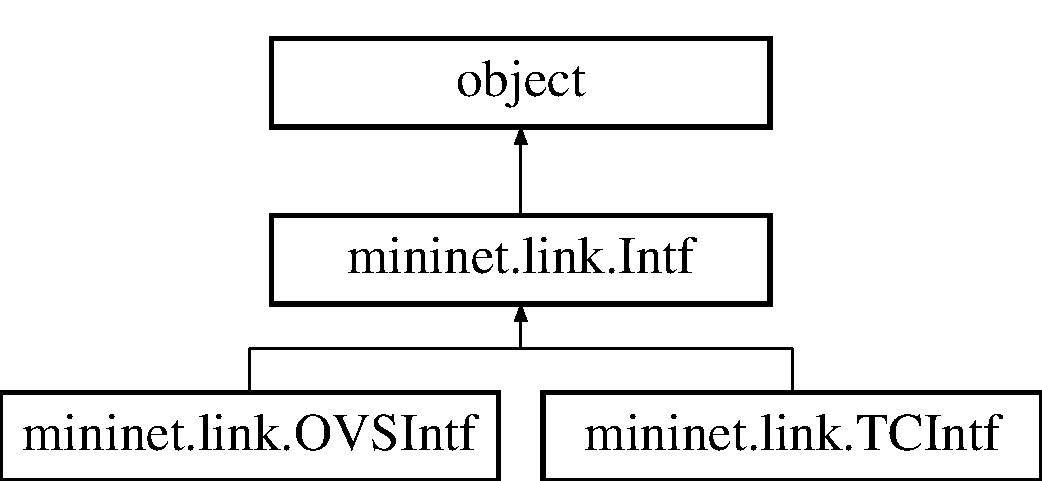
\includegraphics[height=3.000000cm]{classmininet_1_1link_1_1Intf}
\end{center}
\end{figure}
\subsection*{Public Member Functions}
\begin{DoxyCompactItemize}
\item 
def \hyperlink{classmininet_1_1link_1_1Intf_ac3708a345a8200074187a926ab875926}{\-\_\-\-\_\-init\-\_\-\-\_\-}
\item 
\hypertarget{classmininet_1_1link_1_1Intf_aa5178173be205e3ab5e53f950c42f937}{def {\bfseries cmd}}\label{classmininet_1_1link_1_1Intf_aa5178173be205e3ab5e53f950c42f937}

\item 
\hypertarget{classmininet_1_1link_1_1Intf_ac55a9b13b8619e83dfb7709a79183257}{def {\bfseries ifconfig}}\label{classmininet_1_1link_1_1Intf_ac55a9b13b8619e83dfb7709a79183257}

\item 
def \hyperlink{classmininet_1_1link_1_1Intf_ac9e461d9946cf8b2f12657da56f94001}{set\-I\-P}
\item 
def \hyperlink{classmininet_1_1link_1_1Intf_a7676b089cc7d957a0f46d8536fc463ff}{set\-M\-A\-C}
\item 
\hypertarget{classmininet_1_1link_1_1Intf_a915bcdd813ad97ed1318adc0a677cf7d}{def {\bfseries update\-I\-P}}\label{classmininet_1_1link_1_1Intf_a915bcdd813ad97ed1318adc0a677cf7d}

\item 
\hypertarget{classmininet_1_1link_1_1Intf_a31c76efcfc79c0a68abab3be7be2cfc2}{def {\bfseries update\-M\-A\-C}}\label{classmininet_1_1link_1_1Intf_a31c76efcfc79c0a68abab3be7be2cfc2}

\item 
\hypertarget{classmininet_1_1link_1_1Intf_aec843acd406ca8d8a61587cb2ad4e5f3}{def {\bfseries update\-Addr}}\label{classmininet_1_1link_1_1Intf_aec843acd406ca8d8a61587cb2ad4e5f3}

\item 
\hypertarget{classmininet_1_1link_1_1Intf_a151d6511ff83dbc2496d468a265da37e}{def {\bfseries I\-P}}\label{classmininet_1_1link_1_1Intf_a151d6511ff83dbc2496d468a265da37e}

\item 
\hypertarget{classmininet_1_1link_1_1Intf_a2201144993f114c7ba335cfeb0322ecc}{def {\bfseries M\-A\-C}}\label{classmininet_1_1link_1_1Intf_a2201144993f114c7ba335cfeb0322ecc}

\item 
\hypertarget{classmininet_1_1link_1_1Intf_a22278c7e6f880a0cf8a4b3bb40061417}{def {\bfseries is\-Up}}\label{classmininet_1_1link_1_1Intf_a22278c7e6f880a0cf8a4b3bb40061417}

\item 
\hypertarget{classmininet_1_1link_1_1Intf_a4c19501112bfd02d35e4158f8add7585}{def {\bfseries rename}}\label{classmininet_1_1link_1_1Intf_a4c19501112bfd02d35e4158f8add7585}

\item 
def \hyperlink{classmininet_1_1link_1_1Intf_a5f0da363271b067fca43fb3fb6c22923}{set\-Param}
\item 
def \hyperlink{classmininet_1_1link_1_1Intf_a7b2716be97eb1d47d7ee2615497dd2b7}{config}
\item 
\hypertarget{classmininet_1_1link_1_1Intf_afae9a974cbc5bfb288d1d34f41c5d807}{def {\bfseries ssid}}\label{classmininet_1_1link_1_1Intf_afae9a974cbc5bfb288d1d34f41c5d807}

\item 
def \hyperlink{classmininet_1_1link_1_1Intf_a2e4060c80a201cfb7c7e590e84981ae5}{get\-Mac\-Address}
\item 
\hypertarget{classmininet_1_1link_1_1Intf_aa1cacb25148cb3855ebc54f87acb9dc8}{def {\bfseries confirm\-Mesh\-Association}}\label{classmininet_1_1link_1_1Intf_aa1cacb25148cb3855ebc54f87acb9dc8}

\item 
\hypertarget{classmininet_1_1link_1_1Intf_a1b82716226605ea04916dba21e89a099}{def {\bfseries confirm\-Adhoc\-Association}}\label{classmininet_1_1link_1_1Intf_a1b82716226605ea04916dba21e89a099}

\item 
\hypertarget{classmininet_1_1link_1_1Intf_a351d786ebf6119d3da92d9015e3b43a5}{def {\bfseries delete}}\label{classmininet_1_1link_1_1Intf_a351d786ebf6119d3da92d9015e3b43a5}

\item 
\hypertarget{classmininet_1_1link_1_1Intf_aef96c036fb37a79966054ecabf427aaa}{def {\bfseries status}}\label{classmininet_1_1link_1_1Intf_aef96c036fb37a79966054ecabf427aaa}

\item 
\hypertarget{classmininet_1_1link_1_1Intf_a9caa12a6b1330b5a56314d9ef8ea1b5c}{def {\bfseries \-\_\-\-\_\-repr\-\_\-\-\_\-}}\label{classmininet_1_1link_1_1Intf_a9caa12a6b1330b5a56314d9ef8ea1b5c}

\item 
\hypertarget{classmininet_1_1link_1_1Intf_a7aecfa23d31f7e096c4b583e0962ec51}{def {\bfseries \-\_\-\-\_\-str\-\_\-\-\_\-}}\label{classmininet_1_1link_1_1Intf_a7aecfa23d31f7e096c4b583e0962ec51}

\end{DoxyCompactItemize}
\subsection*{Public Attributes}
\begin{DoxyCompactItemize}
\item 
\hypertarget{classmininet_1_1link_1_1Intf_a3206a45ba70e4e592ed30c45e5d17f6f}{{\bfseries node}}\label{classmininet_1_1link_1_1Intf_a3206a45ba70e4e592ed30c45e5d17f6f}

\item 
\hypertarget{classmininet_1_1link_1_1Intf_ad5bbef8077be3827ea0618a1b163566c}{{\bfseries name}}\label{classmininet_1_1link_1_1Intf_ad5bbef8077be3827ea0618a1b163566c}

\item 
\hypertarget{classmininet_1_1link_1_1Intf_ab92af7b0b48343533dc73fe8c71b28ac}{{\bfseries link}}\label{classmininet_1_1link_1_1Intf_ab92af7b0b48343533dc73fe8c71b28ac}

\item 
\hypertarget{classmininet_1_1link_1_1Intf_ad7c0583272110f7473618deb397f37c5}{{\bfseries port}}\label{classmininet_1_1link_1_1Intf_ad7c0583272110f7473618deb397f37c5}

\item 
\hypertarget{classmininet_1_1link_1_1Intf_af578a0cfb3a239569d812380efd35965}{{\bfseries mac}}\label{classmininet_1_1link_1_1Intf_af578a0cfb3a239569d812380efd35965}

\item 
\hypertarget{classmininet_1_1link_1_1Intf_adcdf104877c75870025a0c3960c77273}{{\bfseries iface}}\label{classmininet_1_1link_1_1Intf_adcdf104877c75870025a0c3960c77273}

\item 
\hypertarget{classmininet_1_1link_1_1Intf_ac409149d27b60a9a4f001770e6f055b1}{{\bfseries sta}}\label{classmininet_1_1link_1_1Intf_ac409149d27b60a9a4f001770e6f055b1}

\item 
\hypertarget{classmininet_1_1link_1_1Intf_a232b1a7bb641e23c942682096bd3732e}{{\bfseries prefix\-Len}}\label{classmininet_1_1link_1_1Intf_a232b1a7bb641e23c942682096bd3732e}

\item 
\hypertarget{classmininet_1_1link_1_1Intf_aa8407ce2a3df1a07559516f02bcf8ba9}{{\bfseries ip}}\label{classmininet_1_1link_1_1Intf_aa8407ce2a3df1a07559516f02bcf8ba9}

\item 
\hypertarget{classmininet_1_1link_1_1Intf_ad3f6f4555736b616bb7ddeb66173d3ba}{{\bfseries params}}\label{classmininet_1_1link_1_1Intf_ad3f6f4555736b616bb7ddeb66173d3ba}

\end{DoxyCompactItemize}


\subsection{Constructor \& Destructor Documentation}
\hypertarget{classmininet_1_1link_1_1Intf_ac3708a345a8200074187a926ab875926}{\index{mininet\-::link\-::\-Intf@{mininet\-::link\-::\-Intf}!\-\_\-\-\_\-init\-\_\-\-\_\-@{\-\_\-\-\_\-init\-\_\-\-\_\-}}
\index{\-\_\-\-\_\-init\-\_\-\-\_\-@{\-\_\-\-\_\-init\-\_\-\-\_\-}!mininet::link::Intf@{mininet\-::link\-::\-Intf}}
\subsubsection[{\-\_\-\-\_\-init\-\_\-\-\_\-}]{\setlength{\rightskip}{0pt plus 5cm}def mininet.\-link.\-Intf.\-\_\-\-\_\-init\-\_\-\-\_\- (
\begin{DoxyParamCaption}
\item[{}]{self, }
\item[{}]{name, }
\item[{}]{node = {\ttfamily None}, }
\item[{}]{port = {\ttfamily None}, }
\item[{}]{link = {\ttfamily None}, }
\item[{}]{mac = {\ttfamily None}, }
\item[{}]{params}
\end{DoxyParamCaption}
)}}\label{classmininet_1_1link_1_1Intf_ac3708a345a8200074187a926ab875926}
\begin{DoxyVerb}name: interface name (e.g. h1-eth0)
   node: owning node (where this intf most likely lives)
   link: parent link if we're part of a link
   other arguments are passed to config()\end{DoxyVerb}
 

\subsection{Member Function Documentation}
\hypertarget{classmininet_1_1link_1_1Intf_a7b2716be97eb1d47d7ee2615497dd2b7}{\index{mininet\-::link\-::\-Intf@{mininet\-::link\-::\-Intf}!config@{config}}
\index{config@{config}!mininet::link::Intf@{mininet\-::link\-::\-Intf}}
\subsubsection[{config}]{\setlength{\rightskip}{0pt plus 5cm}def mininet.\-link.\-Intf.\-config (
\begin{DoxyParamCaption}
\item[{}]{self, }
\item[{}]{mac = {\ttfamily None}, }
\item[{}]{ip = {\ttfamily None}, }
\item[{}]{ifconfig = {\ttfamily None}, }
\item[{}]{ssid = {\ttfamily None}, }
\item[{}]{sta = {\ttfamily None}, }
\item[{}]{up = {\ttfamily True}, }
\item[{}]{\-\_\-params}
\end{DoxyParamCaption}
)}}\label{classmininet_1_1link_1_1Intf_a7b2716be97eb1d47d7ee2615497dd2b7}
\begin{DoxyVerb}Configure Node according to (optional) parameters:
   mac: MAC address
   ip: IP address
   ifconfig: arbitrary interface configuration
   Subclasses should override this method and call
   the parent class's config(**params)\end{DoxyVerb}
 \hypertarget{classmininet_1_1link_1_1Intf_a2e4060c80a201cfb7c7e590e84981ae5}{\index{mininet\-::link\-::\-Intf@{mininet\-::link\-::\-Intf}!get\-Mac\-Address@{get\-Mac\-Address}}
\index{get\-Mac\-Address@{get\-Mac\-Address}!mininet::link::Intf@{mininet\-::link\-::\-Intf}}
\subsubsection[{get\-Mac\-Address}]{\setlength{\rightskip}{0pt plus 5cm}def mininet.\-link.\-Intf.\-get\-Mac\-Address (
\begin{DoxyParamCaption}
\item[{}]{self, }
\item[{}]{sta, }
\item[{}]{iface, }
\item[{}]{wlan}
\end{DoxyParamCaption}
)}}\label{classmininet_1_1link_1_1Intf_a2e4060c80a201cfb7c7e590e84981ae5}
\begin{DoxyVerb}get Mac Address of any Interface \end{DoxyVerb}
 \hypertarget{classmininet_1_1link_1_1Intf_ac9e461d9946cf8b2f12657da56f94001}{\index{mininet\-::link\-::\-Intf@{mininet\-::link\-::\-Intf}!set\-I\-P@{set\-I\-P}}
\index{set\-I\-P@{set\-I\-P}!mininet::link::Intf@{mininet\-::link\-::\-Intf}}
\subsubsection[{set\-I\-P}]{\setlength{\rightskip}{0pt plus 5cm}def mininet.\-link.\-Intf.\-set\-I\-P (
\begin{DoxyParamCaption}
\item[{}]{self, }
\item[{}]{ipstr, }
\item[{}]{prefix\-Len = {\ttfamily None}}
\end{DoxyParamCaption}
)}}\label{classmininet_1_1link_1_1Intf_ac9e461d9946cf8b2f12657da56f94001}
\begin{DoxyVerb}Set our IP address\end{DoxyVerb}
 \hypertarget{classmininet_1_1link_1_1Intf_a7676b089cc7d957a0f46d8536fc463ff}{\index{mininet\-::link\-::\-Intf@{mininet\-::link\-::\-Intf}!set\-M\-A\-C@{set\-M\-A\-C}}
\index{set\-M\-A\-C@{set\-M\-A\-C}!mininet::link::Intf@{mininet\-::link\-::\-Intf}}
\subsubsection[{set\-M\-A\-C}]{\setlength{\rightskip}{0pt plus 5cm}def mininet.\-link.\-Intf.\-set\-M\-A\-C (
\begin{DoxyParamCaption}
\item[{}]{self, }
\item[{}]{macstr}
\end{DoxyParamCaption}
)}}\label{classmininet_1_1link_1_1Intf_a7676b089cc7d957a0f46d8536fc463ff}
\begin{DoxyVerb}Set the MAC address for an interface.
   macstr: MAC address as string\end{DoxyVerb}
 \hypertarget{classmininet_1_1link_1_1Intf_a5f0da363271b067fca43fb3fb6c22923}{\index{mininet\-::link\-::\-Intf@{mininet\-::link\-::\-Intf}!set\-Param@{set\-Param}}
\index{set\-Param@{set\-Param}!mininet::link::Intf@{mininet\-::link\-::\-Intf}}
\subsubsection[{set\-Param}]{\setlength{\rightskip}{0pt plus 5cm}def mininet.\-link.\-Intf.\-set\-Param (
\begin{DoxyParamCaption}
\item[{}]{self, }
\item[{}]{results, }
\item[{}]{method, }
\item[{}]{param}
\end{DoxyParamCaption}
)}}\label{classmininet_1_1link_1_1Intf_a5f0da363271b067fca43fb3fb6c22923}
\begin{DoxyVerb}Internal method: configure a *single* parameter
   results: dict of results to update
   method: config method name
   param: arg=value (ignore if value=None)
   value may also be list or dict\end{DoxyVerb}
 

The documentation for this class was generated from the following file\-:\begin{DoxyCompactItemize}
\item 
link.\-py\end{DoxyCompactItemize}

\hypertarget{classmininet_1_1node_1_1IVSSwitch}{\section{mininet.\-node.\-I\-V\-S\-Switch Class Reference}
\label{classmininet_1_1node_1_1IVSSwitch}\index{mininet.\-node.\-I\-V\-S\-Switch@{mininet.\-node.\-I\-V\-S\-Switch}}
}
Inheritance diagram for mininet.\-node.\-I\-V\-S\-Switch\-:\begin{figure}[H]
\begin{center}
\leavevmode
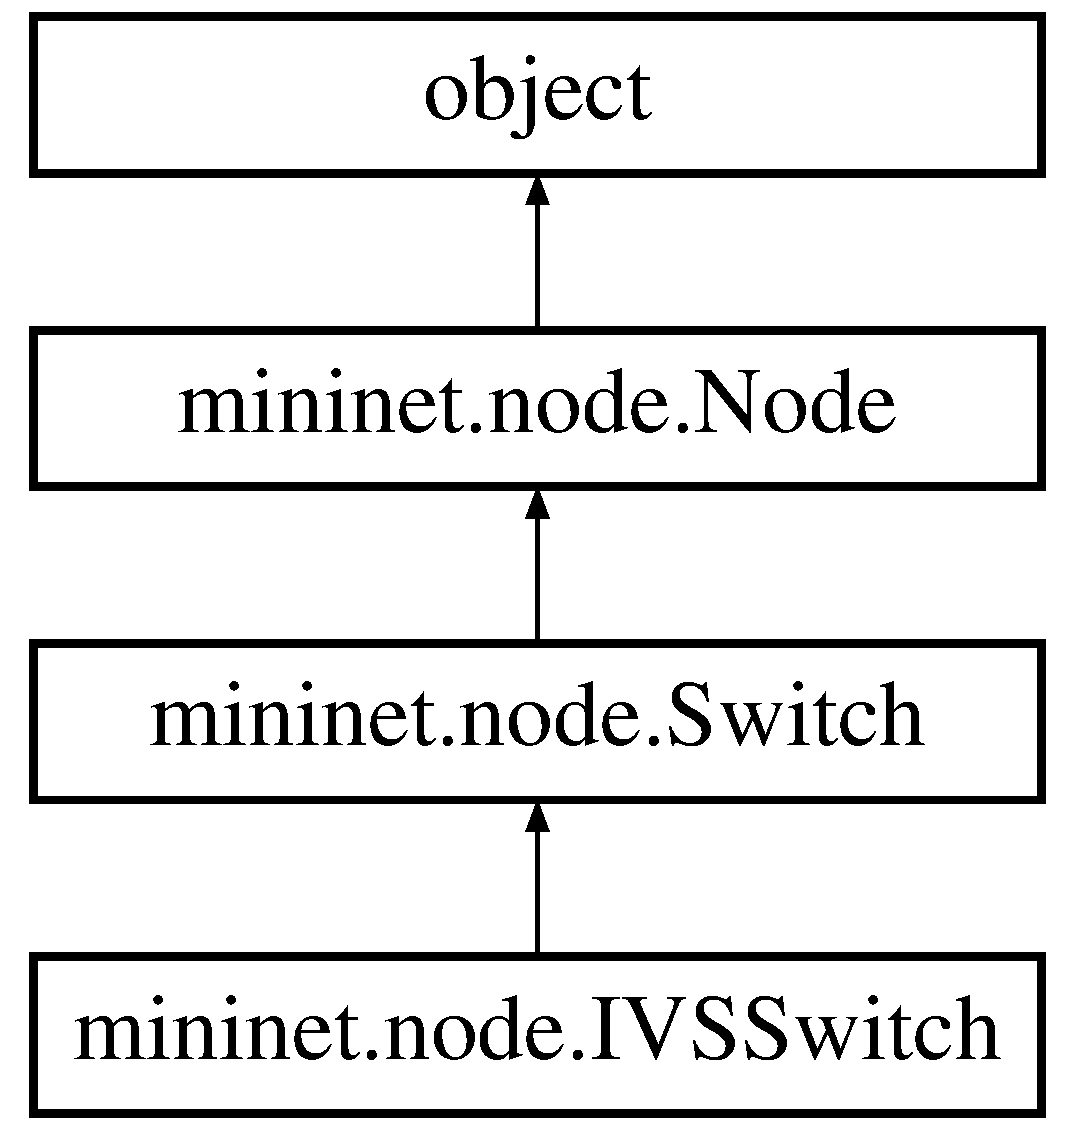
\includegraphics[height=4.000000cm]{classmininet_1_1node_1_1IVSSwitch}
\end{center}
\end{figure}
\subsection*{Public Member Functions}
\begin{DoxyCompactItemize}
\item 
\hypertarget{classmininet_1_1node_1_1IVSSwitch_ace8ef0e200291a6e571eda63da6e3b93}{def {\bfseries \-\_\-\-\_\-init\-\_\-\-\_\-}}\label{classmininet_1_1node_1_1IVSSwitch_ace8ef0e200291a6e571eda63da6e3b93}

\item 
\hypertarget{classmininet_1_1node_1_1IVSSwitch_aefc15cf7c00e207ccbc7d1f26eb0026c}{def {\bfseries setup}}\label{classmininet_1_1node_1_1IVSSwitch_aefc15cf7c00e207ccbc7d1f26eb0026c}

\item 
\hypertarget{classmininet_1_1node_1_1IVSSwitch_a9a235470aa2a49e4b5723b5d2d3eca4b}{def {\bfseries batch\-Shutdown}}\label{classmininet_1_1node_1_1IVSSwitch_a9a235470aa2a49e4b5723b5d2d3eca4b}

\item 
\hypertarget{classmininet_1_1node_1_1IVSSwitch_a149829cffa57ee9966e80953eadb5525}{def {\bfseries start}}\label{classmininet_1_1node_1_1IVSSwitch_a149829cffa57ee9966e80953eadb5525}

\item 
def \hyperlink{classmininet_1_1node_1_1IVSSwitch_a13e63d817d45a1dccce950912adb4764}{stop}
\item 
\hypertarget{classmininet_1_1node_1_1IVSSwitch_af84594ca4a70b42c93aa089791503992}{def {\bfseries attach}}\label{classmininet_1_1node_1_1IVSSwitch_af84594ca4a70b42c93aa089791503992}

\item 
\hypertarget{classmininet_1_1node_1_1IVSSwitch_a52b3b881f18a03f4a6c290c3b58036b6}{def {\bfseries detach}}\label{classmininet_1_1node_1_1IVSSwitch_a52b3b881f18a03f4a6c290c3b58036b6}

\item 
\hypertarget{classmininet_1_1node_1_1IVSSwitch_aac48ff3172eab783da28da5c5dcb7aaf}{def {\bfseries dpctl}}\label{classmininet_1_1node_1_1IVSSwitch_aac48ff3172eab783da28da5c5dcb7aaf}

\end{DoxyCompactItemize}
\subsection*{Public Attributes}
\begin{DoxyCompactItemize}
\item 
\hypertarget{classmininet_1_1node_1_1IVSSwitch_aa3953504c611d5309e888eb1b1be8f9b}{{\bfseries verbose}}\label{classmininet_1_1node_1_1IVSSwitch_aa3953504c611d5309e888eb1b1be8f9b}

\end{DoxyCompactItemize}
\subsection*{Additional Inherited Members}


\subsection{Member Function Documentation}
\hypertarget{classmininet_1_1node_1_1IVSSwitch_a13e63d817d45a1dccce950912adb4764}{\index{mininet\-::node\-::\-I\-V\-S\-Switch@{mininet\-::node\-::\-I\-V\-S\-Switch}!stop@{stop}}
\index{stop@{stop}!mininet::node::IVSSwitch@{mininet\-::node\-::\-I\-V\-S\-Switch}}
\subsubsection[{stop}]{\setlength{\rightskip}{0pt plus 5cm}def mininet.\-node.\-I\-V\-S\-Switch.\-stop (
\begin{DoxyParamCaption}
\item[{}]{self, }
\item[{}]{delete\-Intfs = {\ttfamily True}}
\end{DoxyParamCaption}
)}}\label{classmininet_1_1node_1_1IVSSwitch_a13e63d817d45a1dccce950912adb4764}
\begin{DoxyVerb}Terminate IVS switch.
   deleteIntfs: delete interfaces? (True)\end{DoxyVerb}
 

The documentation for this class was generated from the following file\-:\begin{DoxyCompactItemize}
\item 
node.\-py\end{DoxyCompactItemize}

\hypertarget{classmininet_1_1topo_1_1LinearTopo}{\section{mininet.\-topo.\-Linear\-Topo Class Reference}
\label{classmininet_1_1topo_1_1LinearTopo}\index{mininet.\-topo.\-Linear\-Topo@{mininet.\-topo.\-Linear\-Topo}}
}
Inheritance diagram for mininet.\-topo.\-Linear\-Topo\-:\begin{figure}[H]
\begin{center}
\leavevmode
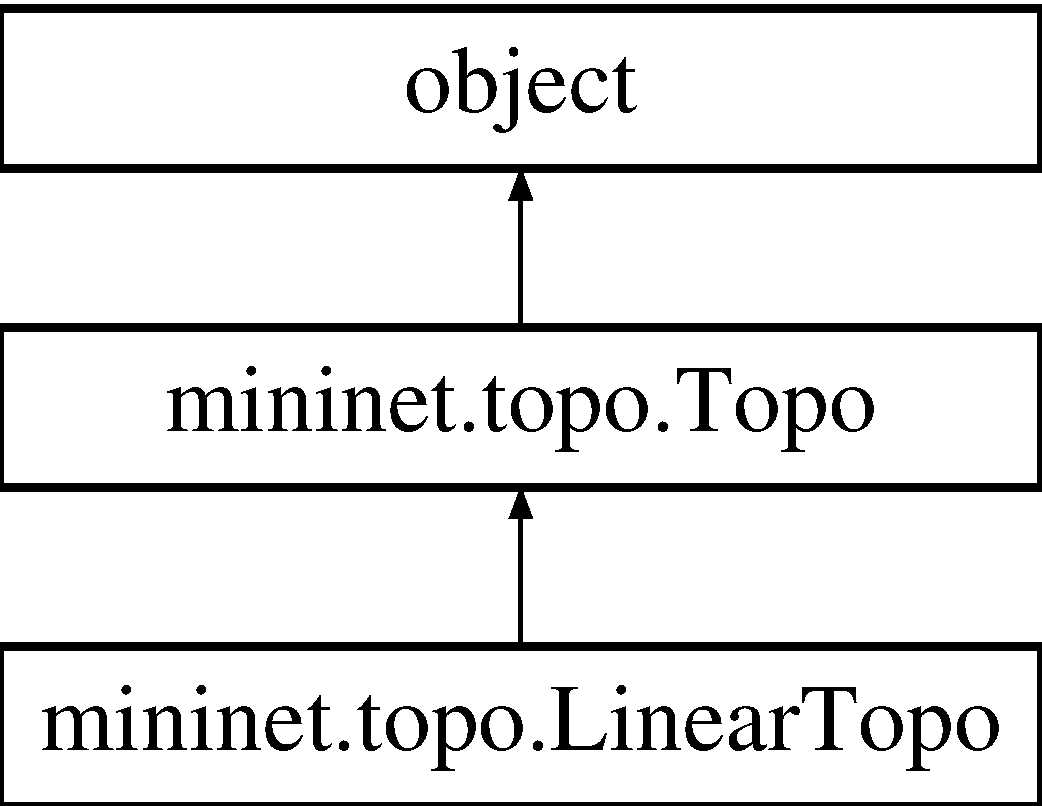
\includegraphics[height=3.000000cm]{classmininet_1_1topo_1_1LinearTopo}
\end{center}
\end{figure}
\subsection*{Public Member Functions}
\begin{DoxyCompactItemize}
\item 
\hypertarget{classmininet_1_1topo_1_1LinearTopo_a152f44c10be70db7bacfc8c48129aff2}{def {\bfseries build}}\label{classmininet_1_1topo_1_1LinearTopo_a152f44c10be70db7bacfc8c48129aff2}

\end{DoxyCompactItemize}
\subsection*{Public Attributes}
\begin{DoxyCompactItemize}
\item 
\hypertarget{classmininet_1_1topo_1_1LinearTopo_abbcd71eec3dfbb630805413552392052}{{\bfseries k}}\label{classmininet_1_1topo_1_1LinearTopo_abbcd71eec3dfbb630805413552392052}

\item 
\hypertarget{classmininet_1_1topo_1_1LinearTopo_ab8389aae5f0a17d3406be12724316ce9}{{\bfseries n}}\label{classmininet_1_1topo_1_1LinearTopo_ab8389aae5f0a17d3406be12724316ce9}

\end{DoxyCompactItemize}
\subsection*{Additional Inherited Members}


The documentation for this class was generated from the following file\-:\begin{DoxyCompactItemize}
\item 
topo.\-py\end{DoxyCompactItemize}

\hypertarget{classmininet_1_1link_1_1Link}{\section{mininet.\-link.\-Link Class Reference}
\label{classmininet_1_1link_1_1Link}\index{mininet.\-link.\-Link@{mininet.\-link.\-Link}}
}
Inheritance diagram for mininet.\-link.\-Link\-:\begin{figure}[H]
\begin{center}
\leavevmode
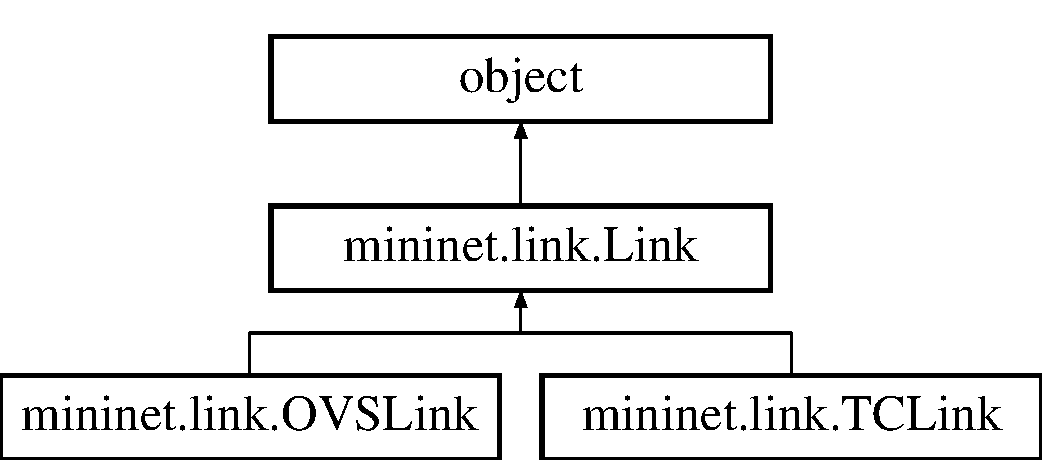
\includegraphics[height=3.000000cm]{classmininet_1_1link_1_1Link}
\end{center}
\end{figure}
\subsection*{Public Member Functions}
\begin{DoxyCompactItemize}
\item 
def \hyperlink{classmininet_1_1link_1_1Link_a05be53888b4da5ffc058c778659296f5}{\-\_\-\-\_\-init\-\_\-\-\_\-}
\item 
\hypertarget{classmininet_1_1link_1_1Link_a7cff25664aad51edfbfa64edfcd832dc}{def {\bfseries wlan\-Name}}\label{classmininet_1_1link_1_1Link_a7cff25664aad51edfbfa64edfcd832dc}

\item 
\hypertarget{classmininet_1_1link_1_1Link_aa3ea9cb1099157f8b8be624a7f2a7bdb}{def {\bfseries intf\-Name}}\label{classmininet_1_1link_1_1Link_aa3ea9cb1099157f8b8be624a7f2a7bdb}

\item 
def \hyperlink{classmininet_1_1link_1_1Link_ade37d7cffeff73830bec0129ac754622}{make\-Intf\-Pair}
\item 
\hypertarget{classmininet_1_1link_1_1Link_a032701855bcb981ae33e5b584d1526cb}{def {\bfseries delete}}\label{classmininet_1_1link_1_1Link_a032701855bcb981ae33e5b584d1526cb}

\item 
\hypertarget{classmininet_1_1link_1_1Link_a00831e1fab1e76169a3af3854f6c2a37}{def {\bfseries stop}}\label{classmininet_1_1link_1_1Link_a00831e1fab1e76169a3af3854f6c2a37}

\item 
\hypertarget{classmininet_1_1link_1_1Link_abbb76b51164c3f279cabc4316e63df34}{def {\bfseries status}}\label{classmininet_1_1link_1_1Link_abbb76b51164c3f279cabc4316e63df34}

\item 
\hypertarget{classmininet_1_1link_1_1Link_ad07f0cb915d250ff63cc6d7dc2f8510b}{def {\bfseries \-\_\-\-\_\-str\-\_\-\-\_\-}}\label{classmininet_1_1link_1_1Link_ad07f0cb915d250ff63cc6d7dc2f8510b}

\end{DoxyCompactItemize}
\subsection*{Public Attributes}
\begin{DoxyCompactItemize}
\item 
\hypertarget{classmininet_1_1link_1_1Link_ae397dc83ab5fec22531b7f0ac7b8bcd8}{{\bfseries fast}}\label{classmininet_1_1link_1_1Link_ae397dc83ab5fec22531b7f0ac7b8bcd8}

\item 
\hypertarget{classmininet_1_1link_1_1Link_a8de28a90dbe9aab0fcca9fcb4d3b0bd8}{{\bfseries intf2}}\label{classmininet_1_1link_1_1Link_a8de28a90dbe9aab0fcca9fcb4d3b0bd8}

\end{DoxyCompactItemize}


\subsection{Detailed Description}
\begin{DoxyVerb}A basic link is just a veth pair.
   Other types of links could be tunnels, link emulators, etc..\end{DoxyVerb}
 

\subsection{Constructor \& Destructor Documentation}
\hypertarget{classmininet_1_1link_1_1Link_a05be53888b4da5ffc058c778659296f5}{\index{mininet\-::link\-::\-Link@{mininet\-::link\-::\-Link}!\-\_\-\-\_\-init\-\_\-\-\_\-@{\-\_\-\-\_\-init\-\_\-\-\_\-}}
\index{\-\_\-\-\_\-init\-\_\-\-\_\-@{\-\_\-\-\_\-init\-\_\-\-\_\-}!mininet::link::Link@{mininet\-::link\-::\-Link}}
\subsubsection[{\-\_\-\-\_\-init\-\_\-\-\_\-}]{\setlength{\rightskip}{0pt plus 5cm}def mininet.\-link.\-Link.\-\_\-\-\_\-init\-\_\-\-\_\- (
\begin{DoxyParamCaption}
\item[{}]{self, }
\item[{}]{node1, }
\item[{}]{node2, }
\item[{}]{port1 = {\ttfamily None}, }
\item[{}]{port2 = {\ttfamily None}, }
\item[{}]{intf\-Name1 = {\ttfamily None}, }
\item[{}]{intf\-Name2 = {\ttfamily None}, }
\item[{}]{addr1 = {\ttfamily None}, }
\item[{}]{addr2 = {\ttfamily None}, }
\item[{}]{intf = {\ttfamily {\bf Intf}}, }
\item[{}]{cls1 = {\ttfamily None}, }
\item[{}]{cls2 = {\ttfamily None}, }
\item[{}]{params1 = {\ttfamily None}, }
\item[{}]{params2 = {\ttfamily None}, }
\item[{}]{fast = {\ttfamily True}, }
\item[{}]{phy\-Iface = {\ttfamily None}}
\end{DoxyParamCaption}
)}}\label{classmininet_1_1link_1_1Link_a05be53888b4da5ffc058c778659296f5}
\begin{DoxyVerb}Create veth link to another node, making two new interfaces.
   node1: first node
   node2: second node
   port1: node1 port number (optional)
   port2: node2 port number (optional)
   intf: default interface class/constructor
   cls1, cls2: optional interface-specific constructors
   intfName1: node1 interface name (optional)
   intfName2: node2  interface name (optional)
   params1: parameters for interface 1
   params2: parameters for interface 2\end{DoxyVerb}
 

\subsection{Member Function Documentation}
\hypertarget{classmininet_1_1link_1_1Link_ade37d7cffeff73830bec0129ac754622}{\index{mininet\-::link\-::\-Link@{mininet\-::link\-::\-Link}!make\-Intf\-Pair@{make\-Intf\-Pair}}
\index{make\-Intf\-Pair@{make\-Intf\-Pair}!mininet::link::Link@{mininet\-::link\-::\-Link}}
\subsubsection[{make\-Intf\-Pair}]{\setlength{\rightskip}{0pt plus 5cm}def mininet.\-link.\-Link.\-make\-Intf\-Pair (
\begin{DoxyParamCaption}
\item[{}]{cls, }
\item[{}]{intfname1, }
\item[{}]{intfname2, }
\item[{}]{addr1 = {\ttfamily None}, }
\item[{}]{addr2 = {\ttfamily None}, }
\item[{}]{node1 = {\ttfamily None}, }
\item[{}]{node2 = {\ttfamily None}, }
\item[{}]{delete\-Intfs = {\ttfamily True}}
\end{DoxyParamCaption}
)}}\label{classmininet_1_1link_1_1Link_ade37d7cffeff73830bec0129ac754622}
\begin{DoxyVerb}Create pair of interfaces
   intfname1: name for interface 1
   intfname2: name for interface 2
   addr1: MAC address for interface 1 (optional)
   addr2: MAC address for interface 2 (optional)
   node1: home node for interface 1 (optional)
   node2: home node for interface 2 (optional)
   (override this method [and possibly delete()]
   to change link type)\end{DoxyVerb}
 

The documentation for this class was generated from the following file\-:\begin{DoxyCompactItemize}
\item 
link.\-py\end{DoxyCompactItemize}

\hypertarget{classmininet_1_1nodelib_1_1LinuxBridge}{\section{mininet.\-nodelib.\-Linux\-Bridge Class Reference}
\label{classmininet_1_1nodelib_1_1LinuxBridge}\index{mininet.\-nodelib.\-Linux\-Bridge@{mininet.\-nodelib.\-Linux\-Bridge}}
}
Inheritance diagram for mininet.\-nodelib.\-Linux\-Bridge\-:\begin{figure}[H]
\begin{center}
\leavevmode
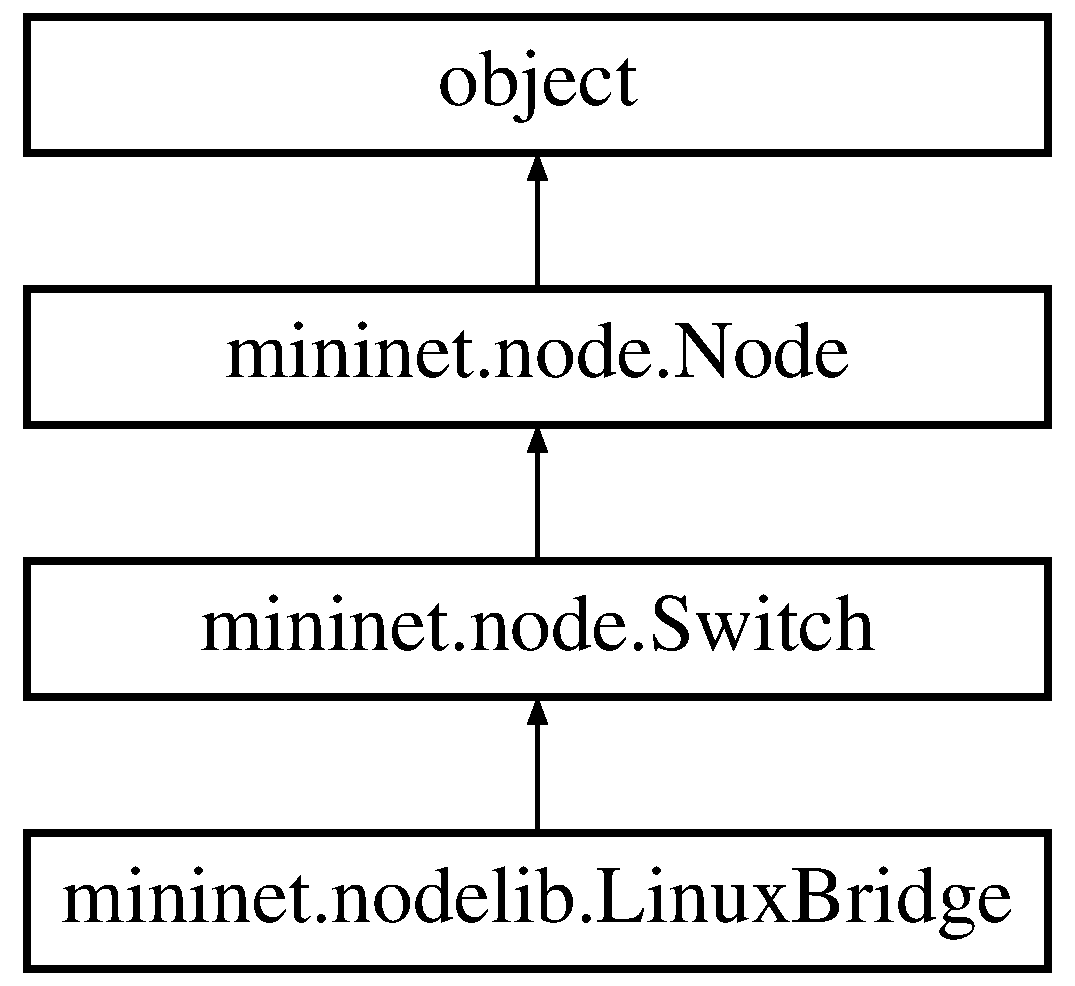
\includegraphics[height=4.000000cm]{classmininet_1_1nodelib_1_1LinuxBridge}
\end{center}
\end{figure}
\subsection*{Public Member Functions}
\begin{DoxyCompactItemize}
\item 
def \hyperlink{classmininet_1_1nodelib_1_1LinuxBridge_a76fa73a4d276034a1d744430a3b03f10}{\-\_\-\-\_\-init\-\_\-\-\_\-}
\item 
\hypertarget{classmininet_1_1nodelib_1_1LinuxBridge_adad4da2be2d09a0c8f80c404e4b2c280}{def {\bfseries connected}}\label{classmininet_1_1nodelib_1_1LinuxBridge_adad4da2be2d09a0c8f80c404e4b2c280}

\item 
\hypertarget{classmininet_1_1nodelib_1_1LinuxBridge_a426f57d257675dd2783eb3233f785bfa}{def {\bfseries start}}\label{classmininet_1_1nodelib_1_1LinuxBridge_a426f57d257675dd2783eb3233f785bfa}

\item 
def \hyperlink{classmininet_1_1nodelib_1_1LinuxBridge_a0c351e04801bc1c3d0c3f2b3916dbc57}{stop}
\item 
\hypertarget{classmininet_1_1nodelib_1_1LinuxBridge_aa561b50171ac27e46f0e8ab7f6060d0c}{def {\bfseries dpctl}}\label{classmininet_1_1nodelib_1_1LinuxBridge_aa561b50171ac27e46f0e8ab7f6060d0c}

\item 
\hypertarget{classmininet_1_1nodelib_1_1LinuxBridge_aec51b470d91325dc41eeb1d05c9fb259}{def {\bfseries setup}}\label{classmininet_1_1nodelib_1_1LinuxBridge_aec51b470d91325dc41eeb1d05c9fb259}

\end{DoxyCompactItemize}
\subsection*{Public Attributes}
\begin{DoxyCompactItemize}
\item 
\hypertarget{classmininet_1_1nodelib_1_1LinuxBridge_a68c1f24f583ceff6be8412926e833bca}{{\bfseries stp}}\label{classmininet_1_1nodelib_1_1LinuxBridge_a68c1f24f583ceff6be8412926e833bca}

\item 
\hypertarget{classmininet_1_1nodelib_1_1LinuxBridge_ac559f0cbb2950c9fe9fbd3bb6d2e2e7c}{{\bfseries prio}}\label{classmininet_1_1nodelib_1_1LinuxBridge_ac559f0cbb2950c9fe9fbd3bb6d2e2e7c}

\end{DoxyCompactItemize}
\subsection*{Static Public Attributes}
\begin{DoxyCompactItemize}
\item 
\hypertarget{classmininet_1_1nodelib_1_1LinuxBridge_a00223ea14134faedec9ccfd12045aeda}{int {\bfseries next\-Prio} = 100}\label{classmininet_1_1nodelib_1_1LinuxBridge_a00223ea14134faedec9ccfd12045aeda}

\end{DoxyCompactItemize}


\subsection{Constructor \& Destructor Documentation}
\hypertarget{classmininet_1_1nodelib_1_1LinuxBridge_a76fa73a4d276034a1d744430a3b03f10}{\index{mininet\-::nodelib\-::\-Linux\-Bridge@{mininet\-::nodelib\-::\-Linux\-Bridge}!\-\_\-\-\_\-init\-\_\-\-\_\-@{\-\_\-\-\_\-init\-\_\-\-\_\-}}
\index{\-\_\-\-\_\-init\-\_\-\-\_\-@{\-\_\-\-\_\-init\-\_\-\-\_\-}!mininet::nodelib::LinuxBridge@{mininet\-::nodelib\-::\-Linux\-Bridge}}
\subsubsection[{\-\_\-\-\_\-init\-\_\-\-\_\-}]{\setlength{\rightskip}{0pt plus 5cm}def mininet.\-nodelib.\-Linux\-Bridge.\-\_\-\-\_\-init\-\_\-\-\_\- (
\begin{DoxyParamCaption}
\item[{}]{self, }
\item[{}]{name, }
\item[{}]{stp = {\ttfamily False}, }
\item[{}]{prio = {\ttfamily None}, }
\item[{}]{kwargs}
\end{DoxyParamCaption}
)}}\label{classmininet_1_1nodelib_1_1LinuxBridge_a76fa73a4d276034a1d744430a3b03f10}
\begin{DoxyVerb}stp: use spanning tree protocol? (default False)
   prio: optional explicit bridge priority for STP\end{DoxyVerb}
 

\subsection{Member Function Documentation}
\hypertarget{classmininet_1_1nodelib_1_1LinuxBridge_a0c351e04801bc1c3d0c3f2b3916dbc57}{\index{mininet\-::nodelib\-::\-Linux\-Bridge@{mininet\-::nodelib\-::\-Linux\-Bridge}!stop@{stop}}
\index{stop@{stop}!mininet::nodelib::LinuxBridge@{mininet\-::nodelib\-::\-Linux\-Bridge}}
\subsubsection[{stop}]{\setlength{\rightskip}{0pt plus 5cm}def mininet.\-nodelib.\-Linux\-Bridge.\-stop (
\begin{DoxyParamCaption}
\item[{}]{self, }
\item[{}]{delete\-Intfs = {\ttfamily True}}
\end{DoxyParamCaption}
)}}\label{classmininet_1_1nodelib_1_1LinuxBridge_a0c351e04801bc1c3d0c3f2b3916dbc57}
\begin{DoxyVerb}Stop Linux bridge
   deleteIntfs: delete interfaces? (True)\end{DoxyVerb}
 

The documentation for this class was generated from the following file\-:\begin{DoxyCompactItemize}
\item 
nodelib.\-py\end{DoxyCompactItemize}

\hypertarget{classmininet_1_1wifiMeshRouting_1_1listNodes}{\section{mininet.\-wifi\-Mesh\-Routing.\-list\-Nodes Class Reference}
\label{classmininet_1_1wifiMeshRouting_1_1listNodes}\index{mininet.\-wifi\-Mesh\-Routing.\-list\-Nodes@{mininet.\-wifi\-Mesh\-Routing.\-list\-Nodes}}
}
Inheritance diagram for mininet.\-wifi\-Mesh\-Routing.\-list\-Nodes\-:\begin{figure}[H]
\begin{center}
\leavevmode
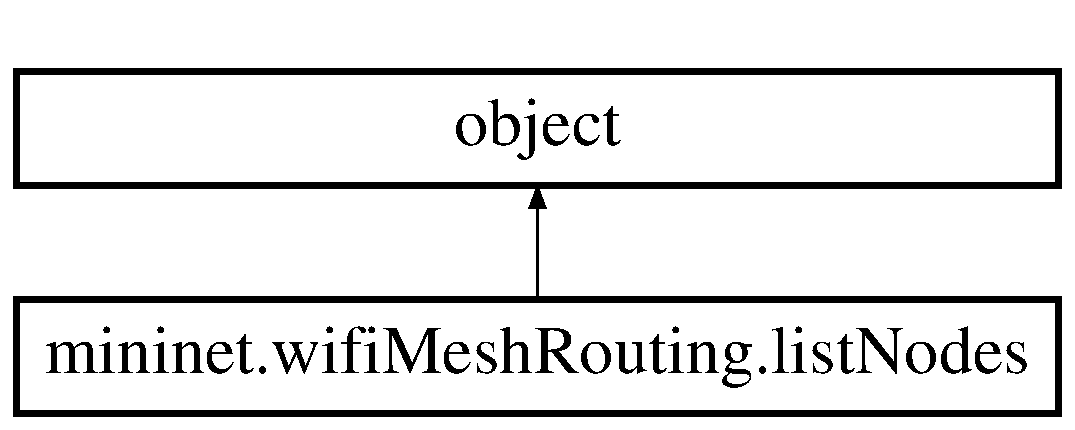
\includegraphics[height=2.000000cm]{classmininet_1_1wifiMeshRouting_1_1listNodes}
\end{center}
\end{figure}
\subsection*{Public Member Functions}
\begin{DoxyCompactItemize}
\item 
\hypertarget{classmininet_1_1wifiMeshRouting_1_1listNodes_a18a31788849ae7900cd38aceafb09e21}{def {\bfseries clear\-List}}\label{classmininet_1_1wifiMeshRouting_1_1listNodes_a18a31788849ae7900cd38aceafb09e21}

\item 
\hypertarget{classmininet_1_1wifiMeshRouting_1_1listNodes_af5acc8dd9646a3e9b458c46abdfd4b7b}{def {\bfseries pairing\-Nodes}}\label{classmininet_1_1wifiMeshRouting_1_1listNodes_af5acc8dd9646a3e9b458c46abdfd4b7b}

\end{DoxyCompactItemize}
\subsection*{Public Attributes}
\begin{DoxyCompactItemize}
\item 
\hypertarget{classmininet_1_1wifiMeshRouting_1_1listNodes_ae811550881969587c24accbaa8652126}{{\bfseries dist}}\label{classmininet_1_1wifiMeshRouting_1_1listNodes_ae811550881969587c24accbaa8652126}

\end{DoxyCompactItemize}
\subsection*{Static Public Attributes}
\begin{DoxyCompactItemize}
\item 
\hypertarget{classmininet_1_1wifiMeshRouting_1_1listNodes_a8acf8072108660d1e9799fda94b489e3}{list {\bfseries nodes\-X} = \mbox{[}$\,$\mbox{]}}\label{classmininet_1_1wifiMeshRouting_1_1listNodes_a8acf8072108660d1e9799fda94b489e3}

\item 
\hypertarget{classmininet_1_1wifiMeshRouting_1_1listNodes_ab9232ee808764f6250ded923fd7026b4}{list {\bfseries nodes\-Y} = \mbox{[}$\,$\mbox{]}}\label{classmininet_1_1wifiMeshRouting_1_1listNodes_ab9232ee808764f6250ded923fd7026b4}

\end{DoxyCompactItemize}


The documentation for this class was generated from the following file\-:\begin{DoxyCompactItemize}
\item 
wifi\-Mesh\-Routing.\-py\end{DoxyCompactItemize}

\hypertarget{classmininet_1_1wifiMeshRouting_1_1meshRouting}{\section{mininet.\-wifi\-Mesh\-Routing.\-mesh\-Routing Class Reference}
\label{classmininet_1_1wifiMeshRouting_1_1meshRouting}\index{mininet.\-wifi\-Mesh\-Routing.\-mesh\-Routing@{mininet.\-wifi\-Mesh\-Routing.\-mesh\-Routing}}
}
Inheritance diagram for mininet.\-wifi\-Mesh\-Routing.\-mesh\-Routing\-:\begin{figure}[H]
\begin{center}
\leavevmode
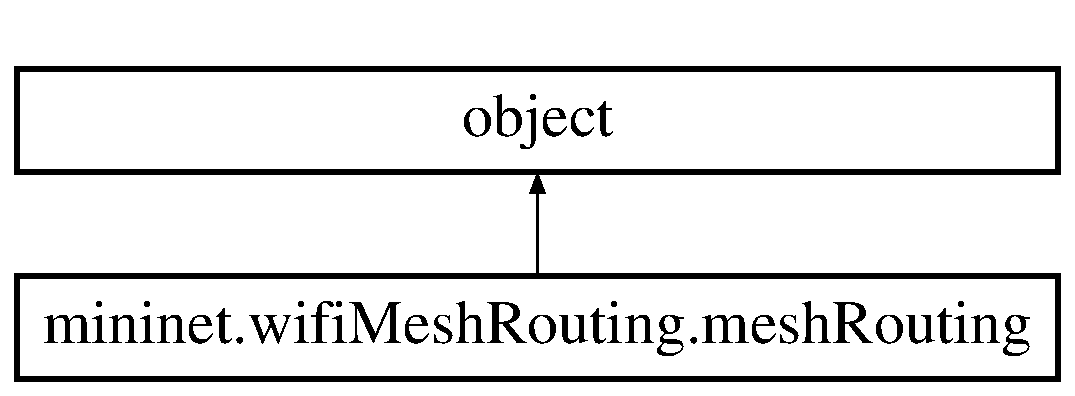
\includegraphics[height=2.000000cm]{classmininet_1_1wifiMeshRouting_1_1meshRouting}
\end{center}
\end{figure}
\subsection*{Public Member Functions}
\begin{DoxyCompactItemize}
\item 
\hypertarget{classmininet_1_1wifiMeshRouting_1_1meshRouting_ab2ff66eaf74f314c9a3c87283a5b6f95}{def {\bfseries custom\-Mesh\-Routing}}\label{classmininet_1_1wifiMeshRouting_1_1meshRouting_ab2ff66eaf74f314c9a3c87283a5b6f95}

\end{DoxyCompactItemize}
\subsection*{Static Public Attributes}
\begin{DoxyCompactItemize}
\item 
\hypertarget{classmininet_1_1wifiMeshRouting_1_1meshRouting_a30cba73b36a7080c264c587a6fe62e06}{string {\bfseries routing} = ''}\label{classmininet_1_1wifiMeshRouting_1_1meshRouting_a30cba73b36a7080c264c587a6fe62e06}

\end{DoxyCompactItemize}


\subsection{Detailed Description}
\begin{DoxyVerb}Mesh Routing\end{DoxyVerb}
 

The documentation for this class was generated from the following file\-:\begin{DoxyCompactItemize}
\item 
wifi\-Mesh\-Routing.\-py\end{DoxyCompactItemize}

\hypertarget{classmininet_1_1topo_1_1MinimalTopo}{\section{mininet.\-topo.\-Minimal\-Topo Class Reference}
\label{classmininet_1_1topo_1_1MinimalTopo}\index{mininet.\-topo.\-Minimal\-Topo@{mininet.\-topo.\-Minimal\-Topo}}
}
Inheritance diagram for mininet.\-topo.\-Minimal\-Topo\-:\begin{figure}[H]
\begin{center}
\leavevmode
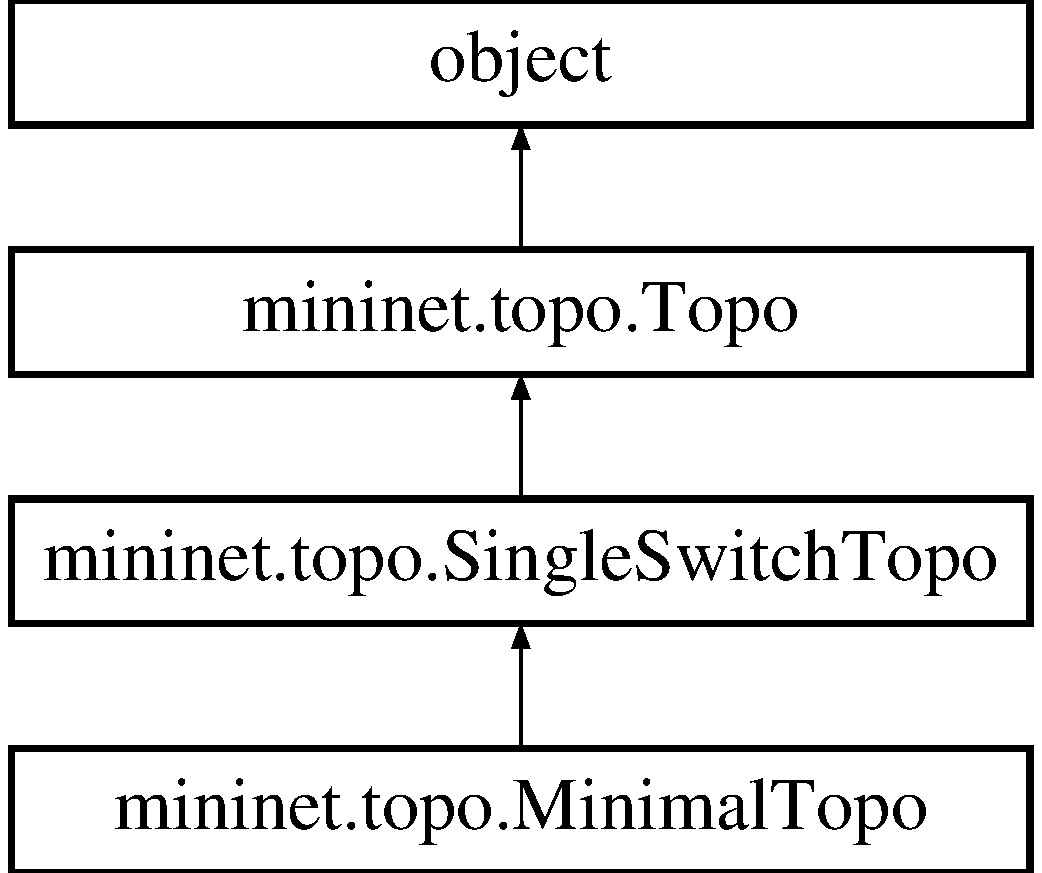
\includegraphics[height=4.000000cm]{classmininet_1_1topo_1_1MinimalTopo}
\end{center}
\end{figure}
\subsection*{Public Member Functions}
\begin{DoxyCompactItemize}
\item 
\hypertarget{classmininet_1_1topo_1_1MinimalTopo_ac7be07b16d7f38e2c1046ea9321c9885}{def {\bfseries build}}\label{classmininet_1_1topo_1_1MinimalTopo_ac7be07b16d7f38e2c1046ea9321c9885}

\end{DoxyCompactItemize}
\subsection*{Additional Inherited Members}


The documentation for this class was generated from the following file\-:\begin{DoxyCompactItemize}
\item 
topo.\-py\end{DoxyCompactItemize}

\hypertarget{classmininet_1_1net_1_1Mininet}{\section{mininet.\-net.\-Mininet Class Reference}
\label{classmininet_1_1net_1_1Mininet}\index{mininet.\-net.\-Mininet@{mininet.\-net.\-Mininet}}
}
Inheritance diagram for mininet.\-net.\-Mininet\-:\begin{figure}[H]
\begin{center}
\leavevmode
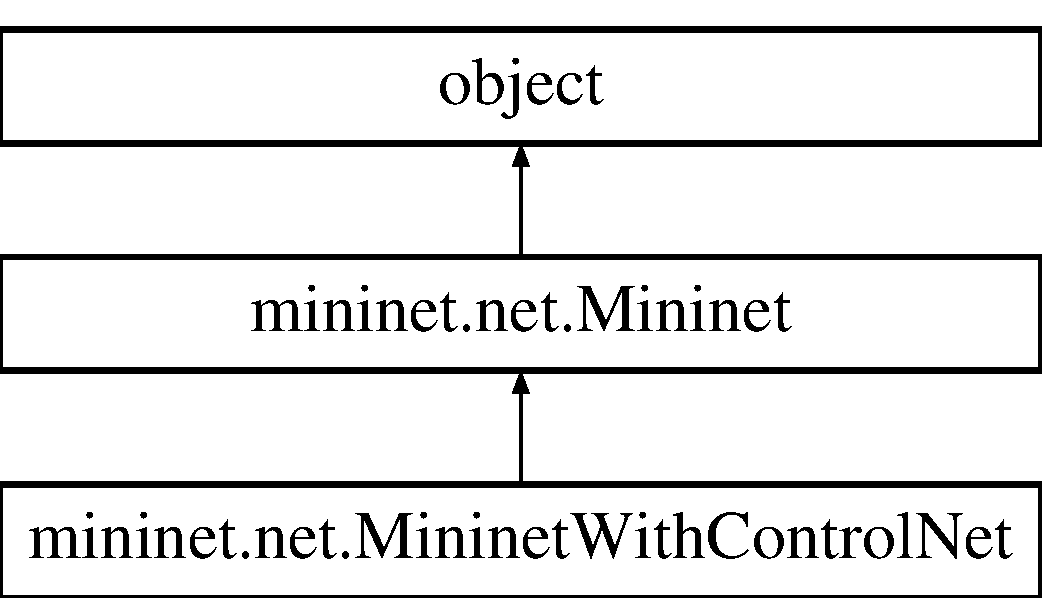
\includegraphics[height=3.000000cm]{classmininet_1_1net_1_1Mininet}
\end{center}
\end{figure}
\subsection*{Public Member Functions}
\begin{DoxyCompactItemize}
\item 
def \hyperlink{classmininet_1_1net_1_1Mininet_a1ed0f0c8ba06a398e02f3952cc4c8393}{\-\_\-\-\_\-init\-\_\-\-\_\-}
\item 
def \hyperlink{classmininet_1_1net_1_1Mininet_ac96ae3d7c168df6c32cbd8a2a1a5a6fe}{wait\-Connected}
\item 
def \hyperlink{classmininet_1_1net_1_1Mininet_aaf25d268b50efdfc7e6c2f4e5e940168}{add\-Host}
\item 
def \hyperlink{classmininet_1_1net_1_1Mininet_aef34acef029345ac8c6fb5860719b103}{add\-Station}
\item 
def \hyperlink{classmininet_1_1net_1_1Mininet_a879cfb9e1c99187836cbfc3fd034645f}{add\-Vehicle}
\item 
def \hyperlink{classmininet_1_1net_1_1Mininet_a271d2c78fc3b8d6e54220ca1f2fd57c4}{add\-Base\-Station}
\item 
def \hyperlink{classmininet_1_1net_1_1Mininet_a7b3e0a0b6a02333067e9d6de5fb0c36a}{add\-Physical\-Base\-Station}
\item 
def \hyperlink{classmininet_1_1net_1_1Mininet_ae4dee4ab63ee9d46bbf3d069dbe9ebbb}{add\-Switch}
\item 
def \hyperlink{classmininet_1_1net_1_1Mininet_aecca42852bcd3f0ef885fa53c07dd2a1}{add\-Controller}
\item 
def \hyperlink{classmininet_1_1net_1_1Mininet_aec5d9c44503b066bf50da7235f622540}{add\-N\-A\-T}
\item 
\hypertarget{classmininet_1_1net_1_1Mininet_a9b0b08399c44a8749c22b6a7e65711a2}{def {\bfseries add\-Of\-Data\-Path}}\label{classmininet_1_1net_1_1Mininet_a9b0b08399c44a8749c22b6a7e65711a2}

\item 
\hypertarget{classmininet_1_1net_1_1Mininet_ab92c0b5ef6f8ee38395753bdceb5fbb2}{def {\bfseries get\-Node\-By\-Name}}\label{classmininet_1_1net_1_1Mininet_ab92c0b5ef6f8ee38395753bdceb5fbb2}

\item 
\hypertarget{classmininet_1_1net_1_1Mininet_aab68ae4924798f60d1b87cc63e6b63ff}{def {\bfseries get}}\label{classmininet_1_1net_1_1Mininet_aab68ae4924798f60d1b87cc63e6b63ff}

\item 
def \hyperlink{classmininet_1_1net_1_1Mininet_a2fe3040d8714f0357b9658820770ee62}{\-\_\-\-\_\-getitem\-\_\-\-\_\-}
\item 
\hypertarget{classmininet_1_1net_1_1Mininet_a3cf367cc6e182457b5bc1db610dbfb3b}{def {\bfseries \-\_\-\-\_\-iter\-\_\-\-\_\-}}\label{classmininet_1_1net_1_1Mininet_a3cf367cc6e182457b5bc1db610dbfb3b}

\item 
\hypertarget{classmininet_1_1net_1_1Mininet_a14fc4b84b7fbb7c478411ae29dba8bbc}{def {\bfseries \-\_\-\-\_\-len\-\_\-\-\_\-}}\label{classmininet_1_1net_1_1Mininet_a14fc4b84b7fbb7c478411ae29dba8bbc}

\item 
\hypertarget{classmininet_1_1net_1_1Mininet_a08e9ac67c0ba7dd43cfc8d00015e1f09}{def {\bfseries \-\_\-\-\_\-contains\-\_\-\-\_\-}}\label{classmininet_1_1net_1_1Mininet_a08e9ac67c0ba7dd43cfc8d00015e1f09}

\item 
\hypertarget{classmininet_1_1net_1_1Mininet_acf4c98ea2f76537309e3c5285ecf4121}{def {\bfseries keys}}\label{classmininet_1_1net_1_1Mininet_acf4c98ea2f76537309e3c5285ecf4121}

\item 
\hypertarget{classmininet_1_1net_1_1Mininet_a8f84d72a3efa668a691b679a87d05fa5}{def {\bfseries values}}\label{classmininet_1_1net_1_1Mininet_a8f84d72a3efa668a691b679a87d05fa5}

\item 
\hypertarget{classmininet_1_1net_1_1Mininet_a8dff5aa7a27a3fe15c7813bcb4032697}{def {\bfseries items}}\label{classmininet_1_1net_1_1Mininet_a8dff5aa7a27a3fe15c7813bcb4032697}

\item 
\hypertarget{classmininet_1_1net_1_1Mininet_a02550962ecf07e20fe0c99e8fb1707de}{def {\bfseries add\-Mesh}}\label{classmininet_1_1net_1_1Mininet_a02550962ecf07e20fe0c99e8fb1707de}

\item 
\hypertarget{classmininet_1_1net_1_1Mininet_a957770ea61e5bdc7c2e285263e6a9d90}{def {\bfseries add\-Hoc}}\label{classmininet_1_1net_1_1Mininet_a957770ea61e5bdc7c2e285263e6a9d90}

\item 
def \hyperlink{classmininet_1_1net_1_1Mininet_aad7b4a355c6b61005588b831c459be87}{configure\-A\-P}
\item 
\hypertarget{classmininet_1_1net_1_1Mininet_a1e20eb4f102a3644eae87bfeed83d27f}{def {\bfseries configure\-Wifi\-Nodes}}\label{classmininet_1_1net_1_1Mininet_a1e20eb4f102a3644eae87bfeed83d27f}

\item 
\hypertarget{classmininet_1_1net_1_1Mininet_ae01361739c8c8a4ab26a6bf12517d541}{def {\bfseries add\-Link}}\label{classmininet_1_1net_1_1Mininet_ae01361739c8c8a4ab26a6bf12517d541}

\item 
\hypertarget{classmininet_1_1net_1_1Mininet_a69cba62f8d87db1d1668aa27876db03a}{def {\bfseries config\-Hosts}}\label{classmininet_1_1net_1_1Mininet_a69cba62f8d87db1d1668aa27876db03a}

\item 
def \hyperlink{classmininet_1_1net_1_1Mininet_a2b42ae2e15dceca476abf8ed9573834c}{build\-From\-Topo}
\item 
\hypertarget{classmininet_1_1net_1_1Mininet_a07e09ac0e7203b02602f62d229f3d144}{def {\bfseries configure\-Control\-Network}}\label{classmininet_1_1net_1_1Mininet_a07e09ac0e7203b02602f62d229f3d144}

\item 
\hypertarget{classmininet_1_1net_1_1Mininet_afccb99c2adc7a06c0bf7a59f4591404e}{def {\bfseries build}}\label{classmininet_1_1net_1_1Mininet_afccb99c2adc7a06c0bf7a59f4591404e}

\item 
\hypertarget{classmininet_1_1net_1_1Mininet_a2392a69351e809e6532e5ae0915a39e9}{def {\bfseries start\-Terms}}\label{classmininet_1_1net_1_1Mininet_a2392a69351e809e6532e5ae0915a39e9}

\item 
\hypertarget{classmininet_1_1net_1_1Mininet_a803d427d23f3de910bd212a21c5fe018}{def {\bfseries stop\-Xterms}}\label{classmininet_1_1net_1_1Mininet_a803d427d23f3de910bd212a21c5fe018}

\item 
\hypertarget{classmininet_1_1net_1_1Mininet_aff78514318d81c6216fdcee11235d73d}{def {\bfseries static\-Arp}}\label{classmininet_1_1net_1_1Mininet_aff78514318d81c6216fdcee11235d73d}

\item 
\hypertarget{classmininet_1_1net_1_1Mininet_a5583fa22f015cecc4796b0560b411957}{def {\bfseries start}}\label{classmininet_1_1net_1_1Mininet_a5583fa22f015cecc4796b0560b411957}

\item 
\hypertarget{classmininet_1_1net_1_1Mininet_a41130182f5aca7b8a63b4d498c27a009}{def {\bfseries seed}}\label{classmininet_1_1net_1_1Mininet_a41130182f5aca7b8a63b4d498c27a009}

\item 
\hypertarget{classmininet_1_1net_1_1Mininet_a89a8cad2aec62cf7927fcf5a764609e6}{def {\bfseries roads}}\label{classmininet_1_1net_1_1Mininet_a89a8cad2aec62cf7927fcf5a764609e6}

\item 
\hypertarget{classmininet_1_1net_1_1Mininet_af7f39fd4e33fa950f83b4da22d228aea}{def {\bfseries stop}}\label{classmininet_1_1net_1_1Mininet_af7f39fd4e33fa950f83b4da22d228aea}

\item 
\hypertarget{classmininet_1_1net_1_1Mininet_a0daaf2248aaf87df61d9e04ca2050935}{def {\bfseries run}}\label{classmininet_1_1net_1_1Mininet_a0daaf2248aaf87df61d9e04ca2050935}

\item 
def \hyperlink{classmininet_1_1net_1_1Mininet_abadd86a33ad9092fee10ce7333471ad7}{monitor}
\item 
def \hyperlink{classmininet_1_1net_1_1Mininet_a5a3d13340db0f440717364e17230512d}{ping}
\item 
def \hyperlink{classmininet_1_1net_1_1Mininet_a36c48a1fed47018152717acf31df8f0b}{ping\-Full}
\item 
def \hyperlink{classmininet_1_1net_1_1Mininet_a4d979e7bbfbee700abd18b4372884f3c}{ping\-All}
\item 
def \hyperlink{classmininet_1_1net_1_1Mininet_a1abd162ba9a3304dd091a2edda1cc4c1}{ping\-Pair}
\item 
def \hyperlink{classmininet_1_1net_1_1Mininet_aed5e30dd177b00c57820f6125784b944}{ping\-All\-Full}
\item 
def \hyperlink{classmininet_1_1net_1_1Mininet_a2e295ea9501bc4c989b1337ddea05f7c}{ping\-Pair\-Full}
\item 
def \hyperlink{classmininet_1_1net_1_1Mininet_a803a1ef9b199402f62e77bd0cce085d4}{iperf}
\item 
def \hyperlink{classmininet_1_1net_1_1Mininet_ade00be5dd4abcf0605b8a8e5f0489272}{run\-Cpu\-Limit\-Test}
\item 
def \hyperlink{classmininet_1_1net_1_1Mininet_a3baedecd9dba7ebb4fdd60c38cee592d}{mobility}
\item 
def \hyperlink{classmininet_1_1net_1_1Mininet_a14d6c3a806e26e7f7dcefb13765d08f4}{start\-Mobility}
\item 
def \hyperlink{classmininet_1_1net_1_1Mininet_a4134cc076d94fbc367b187e85eab4ae0}{stop\-Mobility}
\item 
\hypertarget{classmininet_1_1net_1_1Mininet_ad37986be2169c50f8eb9838987b2a1ac}{def {\bfseries set\-Wifi\-Parameters}}\label{classmininet_1_1net_1_1Mininet_ad37986be2169c50f8eb9838987b2a1ac}

\item 
\hypertarget{classmininet_1_1net_1_1Mininet_adddce43903793291a877203af9d3dbf5}{def {\bfseries use\-External\-Program}}\label{classmininet_1_1net_1_1Mininet_adddce43903793291a877203af9d3dbf5}

\item 
\hypertarget{classmininet_1_1net_1_1Mininet_ad34f3b52c421bd1faf6525b6d765ec21}{def {\bfseries mesh\-Routing}}\label{classmininet_1_1net_1_1Mininet_ad34f3b52c421bd1faf6525b6d765ec21}

\item 
def \hyperlink{classmininet_1_1net_1_1Mininet_a6bae92d0de21dbb8c90a5d862d81daa9}{print\-Distance}
\item 
\hypertarget{classmininet_1_1net_1_1Mininet_ae70c0d26fb295c761b8092fc895c81bf}{def {\bfseries report\-\_\-}}\label{classmininet_1_1net_1_1Mininet_ae70c0d26fb295c761b8092fc895c81bf}

\item 
def \hyperlink{classmininet_1_1net_1_1Mininet_a1a566534520203aafbe1fecd2868c09c}{plot\-Graph}
\item 
def \hyperlink{classmininet_1_1net_1_1Mininet_ab5c13aae58329b94796b9d335ab92874}{get\-Current\-Position}
\item 
def \hyperlink{classmininet_1_1net_1_1Mininet_ad8d38777ffb1dde3484087413f3dcaef}{print\-Position}
\item 
\hypertarget{classmininet_1_1net_1_1Mininet_a84b9e166b58252d6233c040c5f5cd12b}{def {\bfseries propagation\-Model}}\label{classmininet_1_1net_1_1Mininet_a84b9e166b58252d6233c040c5f5cd12b}

\item 
\hypertarget{classmininet_1_1net_1_1Mininet_afa0b6ed0abeca308c5c632ed3b4b714e}{def {\bfseries association\-Control}}\label{classmininet_1_1net_1_1Mininet_afa0b6ed0abeca308c5c632ed3b4b714e}

\item 
def \hyperlink{classmininet_1_1net_1_1Mininet_aa0a3f023a1c24eda79554683e1a9ae08}{device\-Info}
\item 
def \hyperlink{classmininet_1_1net_1_1Mininet_a8288273421854314b24af49d1c0074fa}{get\-Current\-Distance}
\item 
def \hyperlink{classmininet_1_1net_1_1Mininet_a027bfac6f90c3342e6ccd1de63f4591e}{config\-Link\-Status}
\item 
\hypertarget{classmininet_1_1net_1_1Mininet_a6604bea98cddc4f8ca5e8bf6fdb2d0ee}{def {\bfseries interact}}\label{classmininet_1_1net_1_1Mininet_a6604bea98cddc4f8ca5e8bf6fdb2d0ee}

\item 
\hypertarget{classmininet_1_1net_1_1Mininet_a62cf428f7718a375b6246b2995642c2d}{def {\bfseries init}}\label{classmininet_1_1net_1_1Mininet_a62cf428f7718a375b6246b2995642c2d}

\end{DoxyCompactItemize}
\subsection*{Static Public Member Functions}
\begin{DoxyCompactItemize}
\item 
\hypertarget{classmininet_1_1net_1_1Mininet_ae9ded3e770dd6473bc3bc15913572537}{def {\bfseries rand\-Mac}}\label{classmininet_1_1net_1_1Mininet_ae9ded3e770dd6473bc3bc15913572537}

\end{DoxyCompactItemize}
\subsection*{Public Attributes}
\begin{DoxyCompactItemize}
\item 
\hypertarget{classmininet_1_1net_1_1Mininet_a35c89a76ea450f8f6bcd28004affe886}{{\bfseries thread}}\label{classmininet_1_1net_1_1Mininet_a35c89a76ea450f8f6bcd28004affe886}

\item 
\hypertarget{classmininet_1_1net_1_1Mininet_a18eca82d2a2157e0d3f32e5531f9a37b}{{\bfseries topo}}\label{classmininet_1_1net_1_1Mininet_a18eca82d2a2157e0d3f32e5531f9a37b}

\item 
\hypertarget{classmininet_1_1net_1_1Mininet_a70f2ecb1852cb2d773a383b8d22be310}{{\bfseries switch}}\label{classmininet_1_1net_1_1Mininet_a70f2ecb1852cb2d773a383b8d22be310}

\item 
\hypertarget{classmininet_1_1net_1_1Mininet_aeaf2234a107c8e8118d5ee001383170c}{{\bfseries base\-Station}}\label{classmininet_1_1net_1_1Mininet_aeaf2234a107c8e8118d5ee001383170c}

\item 
\hypertarget{classmininet_1_1net_1_1Mininet_ae592bcd15d5cc284e95e9db79eae5c91}{{\bfseries host}}\label{classmininet_1_1net_1_1Mininet_ae592bcd15d5cc284e95e9db79eae5c91}

\item 
\hypertarget{classmininet_1_1net_1_1Mininet_a1fea8c533ff20dabeb5d417b71854aef}{{\bfseries controller}}\label{classmininet_1_1net_1_1Mininet_a1fea8c533ff20dabeb5d417b71854aef}

\item 
\hypertarget{classmininet_1_1net_1_1Mininet_ab73851aa9aa489973e9eb39d949b486b}{{\bfseries link}}\label{classmininet_1_1net_1_1Mininet_ab73851aa9aa489973e9eb39d949b486b}

\item 
\hypertarget{classmininet_1_1net_1_1Mininet_ae78fa197e6d90c2e601aeb9637536872}{{\bfseries intf}}\label{classmininet_1_1net_1_1Mininet_ae78fa197e6d90c2e601aeb9637536872}

\item 
\hypertarget{classmininet_1_1net_1_1Mininet_a6478af80830105810b0cb78decd62128}{{\bfseries ip\-Base}}\label{classmininet_1_1net_1_1Mininet_a6478af80830105810b0cb78decd62128}

\item 
\hypertarget{classmininet_1_1net_1_1Mininet_a4a63d274768ea914a613776f16120e96}{{\bfseries prefix\-Len}}\label{classmininet_1_1net_1_1Mininet_a4a63d274768ea914a613776f16120e96}

\item 
\hypertarget{classmininet_1_1net_1_1Mininet_a5e9423dc4b9f793bb03e432843eedbb9}{{\bfseries next\-I\-P}}\label{classmininet_1_1net_1_1Mininet_a5e9423dc4b9f793bb03e432843eedbb9}

\item 
\hypertarget{classmininet_1_1net_1_1Mininet_aafee98faa2375550fd646a43ee9a5fc4}{{\bfseries in\-Namespace}}\label{classmininet_1_1net_1_1Mininet_aafee98faa2375550fd646a43ee9a5fc4}

\item 
\hypertarget{classmininet_1_1net_1_1Mininet_af0e02fb353f0242c5f5e36f0c4bbc130}{{\bfseries xterms}}\label{classmininet_1_1net_1_1Mininet_af0e02fb353f0242c5f5e36f0c4bbc130}

\item 
\hypertarget{classmininet_1_1net_1_1Mininet_ab235b97a9050402df1ce011350a4b5cf}{{\bfseries cleanup}}\label{classmininet_1_1net_1_1Mininet_ab235b97a9050402df1ce011350a4b5cf}

\item 
\hypertarget{classmininet_1_1net_1_1Mininet_ad643496e04c846c4f23a9c3f0074a48a}{{\bfseries auto\-Set\-Macs}}\label{classmininet_1_1net_1_1Mininet_ad643496e04c846c4f23a9c3f0074a48a}

\item 
\hypertarget{classmininet_1_1net_1_1Mininet_a4556664f3c51078feab9908caf7cc5bd}{{\bfseries auto\-Static\-Arp}}\label{classmininet_1_1net_1_1Mininet_a4556664f3c51078feab9908caf7cc5bd}

\item 
\hypertarget{classmininet_1_1net_1_1Mininet_a9a41167a634aab8db03ce89a78856a77}{{\bfseries auto\-Pin\-Cpus}}\label{classmininet_1_1net_1_1Mininet_a9a41167a634aab8db03ce89a78856a77}

\item 
\hypertarget{classmininet_1_1net_1_1Mininet_a5849d6dda2c1e3350f47de0c56e4189a}{{\bfseries num\-Cores}}\label{classmininet_1_1net_1_1Mininet_a5849d6dda2c1e3350f47de0c56e4189a}

\item 
\hypertarget{classmininet_1_1net_1_1Mininet_a42666c2c8028e07ec47d828bf167c746}{{\bfseries next\-Core}}\label{classmininet_1_1net_1_1Mininet_a42666c2c8028e07ec47d828bf167c746}

\item 
\hypertarget{classmininet_1_1net_1_1Mininet_ac1c6783a435316c9e697964b1df42198}{{\bfseries listen\-Port}}\label{classmininet_1_1net_1_1Mininet_ac1c6783a435316c9e697964b1df42198}

\item 
\hypertarget{classmininet_1_1net_1_1Mininet_a3997458b98745b30b1f3e0e7d736ec9d}{{\bfseries wait\-Conn}}\label{classmininet_1_1net_1_1Mininet_a3997458b98745b30b1f3e0e7d736ec9d}

\item 
\hypertarget{classmininet_1_1net_1_1Mininet_ad6d4dd817be779b28993243391162a68}{{\bfseries start\-\_\-time}}\label{classmininet_1_1net_1_1Mininet_ad6d4dd817be779b28993243391162a68}

\item 
\hypertarget{classmininet_1_1net_1_1Mininet_aec71aba8fcd5a1a758d95ad8bd7c6430}{{\bfseries set\-\_\-seed}}\label{classmininet_1_1net_1_1Mininet_aec71aba8fcd5a1a758d95ad8bd7c6430}

\item 
\hypertarget{classmininet_1_1net_1_1Mininet_a39132e1af0011124b1cc732cbb3fe25c}{{\bfseries nroads}}\label{classmininet_1_1net_1_1Mininet_a39132e1af0011124b1cc732cbb3fe25c}

\item 
\hypertarget{classmininet_1_1net_1_1Mininet_ae04e0d67813f2dd0a91c1eb3d8575855}{{\bfseries first\-Association}}\label{classmininet_1_1net_1_1Mininet_ae04e0d67813f2dd0a91c1eb3d8575855}

\item 
\hypertarget{classmininet_1_1net_1_1Mininet_a843128bf4efbf1484eb0196916b7bb28}{{\bfseries iface\-Configured}}\label{classmininet_1_1net_1_1Mininet_a843128bf4efbf1484eb0196916b7bb28}

\item 
\hypertarget{classmininet_1_1net_1_1Mininet_ab14cc4e9e2dab706a196a99a0ac39018}{{\bfseries is\-Vanet}}\label{classmininet_1_1net_1_1Mininet_ab14cc4e9e2dab706a196a99a0ac39018}

\item 
\hypertarget{classmininet_1_1net_1_1Mininet_a3f6292ff2cbb09f56dd9afdada1e8ae5}{{\bfseries ssid}}\label{classmininet_1_1net_1_1Mininet_a3f6292ff2cbb09f56dd9afdada1e8ae5}

\item 
\hypertarget{classmininet_1_1net_1_1Mininet_ae2496409e64a520419c830fac1821e5b}{{\bfseries mode}}\label{classmininet_1_1net_1_1Mininet_ae2496409e64a520419c830fac1821e5b}

\item 
\hypertarget{classmininet_1_1net_1_1Mininet_a6065a984e3fa85766a09c631853919a7}{{\bfseries channel}}\label{classmininet_1_1net_1_1Mininet_a6065a984e3fa85766a09c631853919a7}

\item 
\hypertarget{classmininet_1_1net_1_1Mininet_a283a512915c4d525c5deb908b4eaa76f}{{\bfseries name\-To\-Node}}\label{classmininet_1_1net_1_1Mininet_a283a512915c4d525c5deb908b4eaa76f}

\item 
\hypertarget{classmininet_1_1net_1_1Mininet_a3ae3ce12f097dacf433874c5fe1da98f}{{\bfseries final\-Position}}\label{classmininet_1_1net_1_1Mininet_a3ae3ce12f097dacf433874c5fe1da98f}

\item 
\hypertarget{classmininet_1_1net_1_1Mininet_a0531a4cc34cb16ad7a74323b0d1bcb2f}{{\bfseries initial\-Position}}\label{classmininet_1_1net_1_1Mininet_a0531a4cc34cb16ad7a74323b0d1bcb2f}

\item 
\hypertarget{classmininet_1_1net_1_1Mininet_afa5c3195ebade2784c9fe0e9713c030f}{{\bfseries access\-Points}}\label{classmininet_1_1net_1_1Mininet_afa5c3195ebade2784c9fe0e9713c030f}

\item 
\hypertarget{classmininet_1_1net_1_1Mininet_af82ccc1227aec42904ebb15495c9ed86}{{\bfseries apexists}}\label{classmininet_1_1net_1_1Mininet_af82ccc1227aec42904ebb15495c9ed86}

\item 
\hypertarget{classmininet_1_1net_1_1Mininet_ae162ea80da91fc5eafdabad308ea7585}{{\bfseries controllers}}\label{classmininet_1_1net_1_1Mininet_ae162ea80da91fc5eafdabad308ea7585}

\item 
\hypertarget{classmininet_1_1net_1_1Mininet_a981203c12672cfa0d031e3fce731c5a7}{{\bfseries hosts}}\label{classmininet_1_1net_1_1Mininet_a981203c12672cfa0d031e3fce731c5a7}

\item 
\hypertarget{classmininet_1_1net_1_1Mininet_a944f0d25b1046160b81153aa61d96326}{{\bfseries links}}\label{classmininet_1_1net_1_1Mininet_a944f0d25b1046160b81153aa61d96326}

\item 
\hypertarget{classmininet_1_1net_1_1Mininet_af4d7ef6952fd773b23205b6a80d60d46}{{\bfseries missing\-Stations}}\label{classmininet_1_1net_1_1Mininet_af4d7ef6952fd773b23205b6a80d60d46}

\item 
\hypertarget{classmininet_1_1net_1_1Mininet_a47aa7a6ef3fccf7c7bac47b1dbeba871}{{\bfseries missing\-Wlan\-A\-P}}\label{classmininet_1_1net_1_1Mininet_a47aa7a6ef3fccf7c7bac47b1dbeba871}

\item 
\hypertarget{classmininet_1_1net_1_1Mininet_a96cdeedd81870ba99c9bb53c4fa5f928}{{\bfseries missing\-Data\-Path}}\label{classmininet_1_1net_1_1Mininet_a96cdeedd81870ba99c9bb53c4fa5f928}

\item 
\hypertarget{classmininet_1_1net_1_1Mininet_a72f2875d94e9f9ed28e287870253ed16}{{\bfseries newapif}}\label{classmininet_1_1net_1_1Mininet_a72f2875d94e9f9ed28e287870253ed16}

\item 
\hypertarget{classmininet_1_1net_1_1Mininet_a95d375c2437090b95912be7c181f52da}{{\bfseries wifi\-Nodes}}\label{classmininet_1_1net_1_1Mininet_a95d375c2437090b95912be7c181f52da}

\item 
\hypertarget{classmininet_1_1net_1_1Mininet_aa31c7aa871d05e533c2a311886608169}{{\bfseries switches}}\label{classmininet_1_1net_1_1Mininet_aa31c7aa871d05e533c2a311886608169}

\item 
\hypertarget{classmininet_1_1net_1_1Mininet_a14022b5fce54808a5451127ebe5aa81f}{{\bfseries stations}}\label{classmininet_1_1net_1_1Mininet_a14022b5fce54808a5451127ebe5aa81f}

\item 
\hypertarget{classmininet_1_1net_1_1Mininet_a12192ba58bf4b0f8b8317c109c1a75e0}{{\bfseries virtual\-Wlan}}\label{classmininet_1_1net_1_1Mininet_a12192ba58bf4b0f8b8317c109c1a75e0}

\item 
\hypertarget{classmininet_1_1net_1_1Mininet_afa6ccc3a452b3b94f7053a9d745a11ab}{{\bfseries fixed\-Position}}\label{classmininet_1_1net_1_1Mininet_afa6ccc3a452b3b94f7053a9d745a11ab}

\item 
\hypertarget{classmininet_1_1net_1_1Mininet_a54d0f994a0804bc43b80d63a559fb1c4}{{\bfseries terms}}\label{classmininet_1_1net_1_1Mininet_a54d0f994a0804bc43b80d63a559fb1c4}

\item 
\hypertarget{classmininet_1_1net_1_1Mininet_a36599be8ee5a16a60851dbe303c3d7c1}{{\bfseries is\-Wi\-Fi}}\label{classmininet_1_1net_1_1Mininet_a36599be8ee5a16a60851dbe303c3d7c1}

\item 
\hypertarget{classmininet_1_1net_1_1Mininet_a5e56360a4f280d0822411659fa355e17}{{\bfseries wifi\-Radios}}\label{classmininet_1_1net_1_1Mininet_a5e56360a4f280d0822411659fa355e17}

\item 
\hypertarget{classmininet_1_1net_1_1Mininet_af8faf0981e0cd37681038089213ff6b2}{{\bfseries built}}\label{classmininet_1_1net_1_1Mininet_af8faf0981e0cd37681038089213ff6b2}

\item 
\hypertarget{classmininet_1_1net_1_1Mininet_a1712944b7a70af57afe325057dfa5e1e}{{\bfseries range}}\label{classmininet_1_1net_1_1Mininet_a1712944b7a70af57afe325057dfa5e1e}

\item 
\hypertarget{classmininet_1_1net_1_1Mininet_a9a2ea86e899a36261ac7e21d2d547467}{{\bfseries bw}}\label{classmininet_1_1net_1_1Mininet_a9a2ea86e899a36261ac7e21d2d547467}

\item 
\hypertarget{classmininet_1_1net_1_1Mininet_a81d0f181cac0bbc56854bdb896fbc3ff}{{\bfseries auth\-\_\-algs}}\label{classmininet_1_1net_1_1Mininet_a81d0f181cac0bbc56854bdb896fbc3ff}

\item 
\hypertarget{classmininet_1_1net_1_1Mininet_a6038aa51044306de6ddc3564f1884435}{{\bfseries wpa}}\label{classmininet_1_1net_1_1Mininet_a6038aa51044306de6ddc3564f1884435}

\item 
\hypertarget{classmininet_1_1net_1_1Mininet_a9c1720f14524c601464e3db4e28c3e9b}{{\bfseries wpa\-\_\-key\-\_\-mgmt}}\label{classmininet_1_1net_1_1Mininet_a9c1720f14524c601464e3db4e28c3e9b}

\item 
\hypertarget{classmininet_1_1net_1_1Mininet_af11f2292a30383d226490e51ab4075b2}{{\bfseries rsn\-\_\-pairwise}}\label{classmininet_1_1net_1_1Mininet_af11f2292a30383d226490e51ab4075b2}

\item 
\hypertarget{classmininet_1_1net_1_1Mininet_a489cc6dc8b1b4e70963f050f2c7a7a06}{{\bfseries wpa\-\_\-passphrase}}\label{classmininet_1_1net_1_1Mininet_a489cc6dc8b1b4e70963f050f2c7a7a06}

\item 
\hypertarget{classmininet_1_1net_1_1Mininet_a2b6ba8d0632a8895afddd10a1abe975e}{{\bfseries wep\-\_\-key0}}\label{classmininet_1_1net_1_1Mininet_a2b6ba8d0632a8895afddd10a1abe975e}

\item 
\hypertarget{classmininet_1_1net_1_1Mininet_a58484102ec46071c8f8af1e25db40176}{{\bfseries country\-\_\-code}}\label{classmininet_1_1net_1_1Mininet_a58484102ec46071c8f8af1e25db40176}

\item 
\hypertarget{classmininet_1_1net_1_1Mininet_a86a8bf39b73e68a05d5b510acc370f5d}{{\bfseries wmm\-\_\-enabled}}\label{classmininet_1_1net_1_1Mininet_a86a8bf39b73e68a05d5b510acc370f5d}

\item 
\hypertarget{classmininet_1_1net_1_1Mininet_a89e1711664ad277b7c121b6e2a6f1adc}{{\bfseries node}}\label{classmininet_1_1net_1_1Mininet_a89e1711664ad277b7c121b6e2a6f1adc}

\item 
\hypertarget{classmininet_1_1net_1_1Mininet_a4ace2969c4abb59b26b3610179c997b8}{{\bfseries stage}}\label{classmininet_1_1net_1_1Mininet_a4ace2969c4abb59b26b3610179c997b8}

\item 
\hypertarget{classmininet_1_1net_1_1Mininet_ab86c5f213bcbd5c1ea13cf45b7fcfc86}{{\bfseries time}}\label{classmininet_1_1net_1_1Mininet_ab86c5f213bcbd5c1ea13cf45b7fcfc86}

\item 
\hypertarget{classmininet_1_1net_1_1Mininet_ac5906f7c56faf8063fea24c9056100b9}{{\bfseries mobility\-Model}}\label{classmininet_1_1net_1_1Mininet_ac5906f7c56faf8063fea24c9056100b9}

\item 
\hypertarget{classmininet_1_1net_1_1Mininet_aba20ed4cd5a64bb2133d11363527e734}{{\bfseries sta\-Mov}}\label{classmininet_1_1net_1_1Mininet_aba20ed4cd5a64bb2133d11363527e734}

\item 
\hypertarget{classmininet_1_1net_1_1Mininet_a807e52789ce35d7a43c76808cf96a800}{{\bfseries pos\-\_\-x}}\label{classmininet_1_1net_1_1Mininet_a807e52789ce35d7a43c76808cf96a800}

\item 
\hypertarget{classmininet_1_1net_1_1Mininet_a0577d1f66795ceec5787a0234c971456}{{\bfseries pos\-\_\-y}}\label{classmininet_1_1net_1_1Mininet_a0577d1f66795ceec5787a0234c971456}

\item 
\hypertarget{classmininet_1_1net_1_1Mininet_a7407c121fa7823b87358fb917ce6c566}{{\bfseries pos\-\_\-z}}\label{classmininet_1_1net_1_1Mininet_a7407c121fa7823b87358fb917ce6c566}

\end{DoxyCompactItemize}
\subsection*{Static Public Attributes}
\begin{DoxyCompactItemize}
\item 
\hypertarget{classmininet_1_1net_1_1Mininet_a26dff81a193e45962b584629f937c0cd}{{\bfseries inited} = False}\label{classmininet_1_1net_1_1Mininet_a26dff81a193e45962b584629f937c0cd}

\end{DoxyCompactItemize}


\subsection{Constructor \& Destructor Documentation}
\hypertarget{classmininet_1_1net_1_1Mininet_a1ed0f0c8ba06a398e02f3952cc4c8393}{\index{mininet\-::net\-::\-Mininet@{mininet\-::net\-::\-Mininet}!\-\_\-\-\_\-init\-\_\-\-\_\-@{\-\_\-\-\_\-init\-\_\-\-\_\-}}
\index{\-\_\-\-\_\-init\-\_\-\-\_\-@{\-\_\-\-\_\-init\-\_\-\-\_\-}!mininet::net::Mininet@{mininet\-::net\-::\-Mininet}}
\subsubsection[{\-\_\-\-\_\-init\-\_\-\-\_\-}]{\setlength{\rightskip}{0pt plus 5cm}def mininet.\-net.\-Mininet.\-\_\-\-\_\-init\-\_\-\-\_\- (
\begin{DoxyParamCaption}
\item[{}]{self, }
\item[{}]{topo = {\ttfamily None}, }
\item[{}]{switch = {\ttfamily OVSKernelSwitch}, }
\item[{}]{host = {\ttfamily Host}, }
\item[{}]{is\-Wi\-Fi = {\ttfamily False}, }
\item[{}]{controller = {\ttfamily DefaultController}, }
\item[{}]{link = {\ttfamily {\bf Link}}, }
\item[{}]{intf = {\ttfamily {\bf Intf}}, }
\item[{}]{wifi\-Radios = {\ttfamily 0}, }
\item[{}]{build = {\ttfamily True}, }
\item[{}]{xterms = {\ttfamily False}, }
\item[{}]{cleanup = {\ttfamily False}, }
\item[{}]{ip\-Base = {\ttfamily '10.0.0.0/8'}, }
\item[{}]{in\-Namespace = {\ttfamily False}, }
\item[{}]{auto\-Set\-Macs = {\ttfamily False}, }
\item[{}]{auto\-Static\-Arp = {\ttfamily False}, }
\item[{}]{auto\-Pin\-Cpus = {\ttfamily False}, }
\item[{}]{listen\-Port = {\ttfamily None}, }
\item[{}]{wait\-Connected = {\ttfamily False}, }
\item[{}]{ssid = {\ttfamily \char`\"{}my-\/ssid\char`\"{}}, }
\item[{}]{mode = {\ttfamily \char`\"{}g\char`\"{}}, }
\item[{}]{channel = {\ttfamily \char`\"{}6\char`\"{}}}
\end{DoxyParamCaption}
)}}\label{classmininet_1_1net_1_1Mininet_a1ed0f0c8ba06a398e02f3952cc4c8393}
\begin{DoxyVerb}Create Mininet object.
   topo: Topo (topology) object or None
   switch: default Switch class
   host: default Host class/constructor
   controller: default Controller class/constructor
   link: default Link class/constructor
   intf: default Intf class/constructor
   ipBase: base IP address for hosts,
   build: build now from topo?
   xterms: if build now, spawn xterms?
   cleanup: if build now, cleanup before creating?
   inNamespace: spawn switches and controller in net namespaces?
   autoSetMacs: set MAC addrs automatically like IP addresses?
   autoStaticArp: set all-pairs static MAC addrs?
   autoPinCpus: pin hosts to (real) cores (requires CPULimitedHost)?
   listenPort: base listening port to open; will be incremented for
       each additional switch in the net if inNamespace=False\end{DoxyVerb}
 

\subsection{Member Function Documentation}
\hypertarget{classmininet_1_1net_1_1Mininet_a2fe3040d8714f0357b9658820770ee62}{\index{mininet\-::net\-::\-Mininet@{mininet\-::net\-::\-Mininet}!\-\_\-\-\_\-getitem\-\_\-\-\_\-@{\-\_\-\-\_\-getitem\-\_\-\-\_\-}}
\index{\-\_\-\-\_\-getitem\-\_\-\-\_\-@{\-\_\-\-\_\-getitem\-\_\-\-\_\-}!mininet::net::Mininet@{mininet\-::net\-::\-Mininet}}
\subsubsection[{\-\_\-\-\_\-getitem\-\_\-\-\_\-}]{\setlength{\rightskip}{0pt plus 5cm}def mininet.\-net.\-Mininet.\-\_\-\-\_\-getitem\-\_\-\-\_\- (
\begin{DoxyParamCaption}
\item[{}]{self, }
\item[{}]{key}
\end{DoxyParamCaption}
)}}\label{classmininet_1_1net_1_1Mininet_a2fe3040d8714f0357b9658820770ee62}
\begin{DoxyVerb}net [ name ] operator: Return node(s) with given name(s)\end{DoxyVerb}
 \hypertarget{classmininet_1_1net_1_1Mininet_a271d2c78fc3b8d6e54220ca1f2fd57c4}{\index{mininet\-::net\-::\-Mininet@{mininet\-::net\-::\-Mininet}!add\-Base\-Station@{add\-Base\-Station}}
\index{add\-Base\-Station@{add\-Base\-Station}!mininet::net::Mininet@{mininet\-::net\-::\-Mininet}}
\subsubsection[{add\-Base\-Station}]{\setlength{\rightskip}{0pt plus 5cm}def mininet.\-net.\-Mininet.\-add\-Base\-Station (
\begin{DoxyParamCaption}
\item[{}]{self, }
\item[{}]{name, }
\item[{}]{cls = {\ttfamily None}, }
\item[{}]{params}
\end{DoxyParamCaption}
)}}\label{classmininet_1_1net_1_1Mininet_a271d2c78fc3b8d6e54220ca1f2fd57c4}
\begin{DoxyVerb}Add BaseStation.
   name: name of basestation to add
   cls: custom switch class/constructor (optional)
   returns: added switch
   side effect: increments listenPort ivar .\end{DoxyVerb}
 \hypertarget{classmininet_1_1net_1_1Mininet_aecca42852bcd3f0ef885fa53c07dd2a1}{\index{mininet\-::net\-::\-Mininet@{mininet\-::net\-::\-Mininet}!add\-Controller@{add\-Controller}}
\index{add\-Controller@{add\-Controller}!mininet::net::Mininet@{mininet\-::net\-::\-Mininet}}
\subsubsection[{add\-Controller}]{\setlength{\rightskip}{0pt plus 5cm}def mininet.\-net.\-Mininet.\-add\-Controller (
\begin{DoxyParamCaption}
\item[{}]{self, }
\item[{}]{name = {\ttfamily 'c0'}, }
\item[{}]{controller = {\ttfamily None}, }
\item[{}]{params}
\end{DoxyParamCaption}
)}}\label{classmininet_1_1net_1_1Mininet_aecca42852bcd3f0ef885fa53c07dd2a1}
\begin{DoxyVerb}Add controller.
   controller: Controller class\end{DoxyVerb}
 \hypertarget{classmininet_1_1net_1_1Mininet_aaf25d268b50efdfc7e6c2f4e5e940168}{\index{mininet\-::net\-::\-Mininet@{mininet\-::net\-::\-Mininet}!add\-Host@{add\-Host}}
\index{add\-Host@{add\-Host}!mininet::net::Mininet@{mininet\-::net\-::\-Mininet}}
\subsubsection[{add\-Host}]{\setlength{\rightskip}{0pt plus 5cm}def mininet.\-net.\-Mininet.\-add\-Host (
\begin{DoxyParamCaption}
\item[{}]{self, }
\item[{}]{name, }
\item[{}]{cls = {\ttfamily None}, }
\item[{}]{params}
\end{DoxyParamCaption}
)}}\label{classmininet_1_1net_1_1Mininet_aaf25d268b50efdfc7e6c2f4e5e940168}
\begin{DoxyVerb}Add host.
   name: name of host to add
   cls: custom host class/constructor (optional)
   params: parameters for host
   returns: added host\end{DoxyVerb}
 \hypertarget{classmininet_1_1net_1_1Mininet_aec5d9c44503b066bf50da7235f622540}{\index{mininet\-::net\-::\-Mininet@{mininet\-::net\-::\-Mininet}!add\-N\-A\-T@{add\-N\-A\-T}}
\index{add\-N\-A\-T@{add\-N\-A\-T}!mininet::net::Mininet@{mininet\-::net\-::\-Mininet}}
\subsubsection[{add\-N\-A\-T}]{\setlength{\rightskip}{0pt plus 5cm}def mininet.\-net.\-Mininet.\-add\-N\-A\-T (
\begin{DoxyParamCaption}
\item[{}]{self, }
\item[{}]{name = {\ttfamily 'nat0'}, }
\item[{}]{connect = {\ttfamily True}, }
\item[{}]{in\-Namespace = {\ttfamily False}, }
\item[{}]{params}
\end{DoxyParamCaption}
)}}\label{classmininet_1_1net_1_1Mininet_aec5d9c44503b066bf50da7235f622540}
\begin{DoxyVerb}Add a NAT to the Mininet network
   name: name of NAT node
   connect: switch to connect to | True (s1) | None
   inNamespace: create in a network namespace
   params: other NAT node params, notably:
       ip: used as default gateway address\end{DoxyVerb}
 \hypertarget{classmininet_1_1net_1_1Mininet_a7b3e0a0b6a02333067e9d6de5fb0c36a}{\index{mininet\-::net\-::\-Mininet@{mininet\-::net\-::\-Mininet}!add\-Physical\-Base\-Station@{add\-Physical\-Base\-Station}}
\index{add\-Physical\-Base\-Station@{add\-Physical\-Base\-Station}!mininet::net::Mininet@{mininet\-::net\-::\-Mininet}}
\subsubsection[{add\-Physical\-Base\-Station}]{\setlength{\rightskip}{0pt plus 5cm}def mininet.\-net.\-Mininet.\-add\-Physical\-Base\-Station (
\begin{DoxyParamCaption}
\item[{}]{self, }
\item[{}]{name, }
\item[{}]{cls = {\ttfamily None}, }
\item[{}]{params}
\end{DoxyParamCaption}
)}}\label{classmininet_1_1net_1_1Mininet_a7b3e0a0b6a02333067e9d6de5fb0c36a}
\begin{DoxyVerb}Add BaseStation.
   name: name of basestation to add
   cls: custom switch class/constructor (optional)
   returns: added switch
   side effect: increments listenPort ivar .\end{DoxyVerb}
 \hypertarget{classmininet_1_1net_1_1Mininet_aef34acef029345ac8c6fb5860719b103}{\index{mininet\-::net\-::\-Mininet@{mininet\-::net\-::\-Mininet}!add\-Station@{add\-Station}}
\index{add\-Station@{add\-Station}!mininet::net::Mininet@{mininet\-::net\-::\-Mininet}}
\subsubsection[{add\-Station}]{\setlength{\rightskip}{0pt plus 5cm}def mininet.\-net.\-Mininet.\-add\-Station (
\begin{DoxyParamCaption}
\item[{}]{self, }
\item[{}]{name, }
\item[{}]{cls = {\ttfamily None}, }
\item[{}]{params}
\end{DoxyParamCaption}
)}}\label{classmininet_1_1net_1_1Mininet_aef34acef029345ac8c6fb5860719b103}
\begin{DoxyVerb}Add Station.
   name: name of station to add
   cls: custom host class/constructor (optional)
   params: parameters for host
   returns: added host\end{DoxyVerb}
 \hypertarget{classmininet_1_1net_1_1Mininet_ae4dee4ab63ee9d46bbf3d069dbe9ebbb}{\index{mininet\-::net\-::\-Mininet@{mininet\-::net\-::\-Mininet}!add\-Switch@{add\-Switch}}
\index{add\-Switch@{add\-Switch}!mininet::net::Mininet@{mininet\-::net\-::\-Mininet}}
\subsubsection[{add\-Switch}]{\setlength{\rightskip}{0pt plus 5cm}def mininet.\-net.\-Mininet.\-add\-Switch (
\begin{DoxyParamCaption}
\item[{}]{self, }
\item[{}]{name, }
\item[{}]{cls = {\ttfamily None}, }
\item[{}]{params}
\end{DoxyParamCaption}
)}}\label{classmininet_1_1net_1_1Mininet_ae4dee4ab63ee9d46bbf3d069dbe9ebbb}
\begin{DoxyVerb}Add switch.
   name: name of switch to add
   cls: custom switch class/constructor (optional)
   returns: added switch
   side effect: increments listenPort ivar .\end{DoxyVerb}
 \hypertarget{classmininet_1_1net_1_1Mininet_a879cfb9e1c99187836cbfc3fd034645f}{\index{mininet\-::net\-::\-Mininet@{mininet\-::net\-::\-Mininet}!add\-Vehicle@{add\-Vehicle}}
\index{add\-Vehicle@{add\-Vehicle}!mininet::net::Mininet@{mininet\-::net\-::\-Mininet}}
\subsubsection[{add\-Vehicle}]{\setlength{\rightskip}{0pt plus 5cm}def mininet.\-net.\-Mininet.\-add\-Vehicle (
\begin{DoxyParamCaption}
\item[{}]{self, }
\item[{}]{name, }
\item[{}]{cls = {\ttfamily None}, }
\item[{}]{params}
\end{DoxyParamCaption}
)}}\label{classmininet_1_1net_1_1Mininet_a879cfb9e1c99187836cbfc3fd034645f}
\begin{DoxyVerb}Add Vehicle.
   name: name of vehicle to add
   cls: custom host class/constructor (optional)
   params: parameters for host
   returns: added host\end{DoxyVerb}
 \hypertarget{classmininet_1_1net_1_1Mininet_a2b42ae2e15dceca476abf8ed9573834c}{\index{mininet\-::net\-::\-Mininet@{mininet\-::net\-::\-Mininet}!build\-From\-Topo@{build\-From\-Topo}}
\index{build\-From\-Topo@{build\-From\-Topo}!mininet::net::Mininet@{mininet\-::net\-::\-Mininet}}
\subsubsection[{build\-From\-Topo}]{\setlength{\rightskip}{0pt plus 5cm}def mininet.\-net.\-Mininet.\-build\-From\-Topo (
\begin{DoxyParamCaption}
\item[{}]{self, }
\item[{}]{topo = {\ttfamily None}}
\end{DoxyParamCaption}
)}}\label{classmininet_1_1net_1_1Mininet_a2b42ae2e15dceca476abf8ed9573834c}
\begin{DoxyVerb}Build mininet from a topology object
   At the end of this function, everything should be connected
   and up.\end{DoxyVerb}
 \hypertarget{classmininet_1_1net_1_1Mininet_a027bfac6f90c3342e6ccd1de63f4591e}{\index{mininet\-::net\-::\-Mininet@{mininet\-::net\-::\-Mininet}!config\-Link\-Status@{config\-Link\-Status}}
\index{config\-Link\-Status@{config\-Link\-Status}!mininet::net::Mininet@{mininet\-::net\-::\-Mininet}}
\subsubsection[{config\-Link\-Status}]{\setlength{\rightskip}{0pt plus 5cm}def mininet.\-net.\-Mininet.\-config\-Link\-Status (
\begin{DoxyParamCaption}
\item[{}]{self, }
\item[{}]{src, }
\item[{}]{dst, }
\item[{}]{status}
\end{DoxyParamCaption}
)}}\label{classmininet_1_1net_1_1Mininet_a027bfac6f90c3342e6ccd1de63f4591e}
\begin{DoxyVerb}Change status of src <-> dst links.
   src: node name
   dst: node name
   status: string {up, down}\end{DoxyVerb}
 \hypertarget{classmininet_1_1net_1_1Mininet_aad7b4a355c6b61005588b831c459be87}{\index{mininet\-::net\-::\-Mininet@{mininet\-::net\-::\-Mininet}!configure\-A\-P@{configure\-A\-P}}
\index{configure\-A\-P@{configure\-A\-P}!mininet::net::Mininet@{mininet\-::net\-::\-Mininet}}
\subsubsection[{configure\-A\-P}]{\setlength{\rightskip}{0pt plus 5cm}def mininet.\-net.\-Mininet.\-configure\-A\-P (
\begin{DoxyParamCaption}
\item[{}]{self}
\end{DoxyParamCaption}
)}}\label{classmininet_1_1net_1_1Mininet_aad7b4a355c6b61005588b831c459be87}
\begin{DoxyVerb}Configure AP\end{DoxyVerb}
 \hypertarget{classmininet_1_1net_1_1Mininet_aa0a3f023a1c24eda79554683e1a9ae08}{\index{mininet\-::net\-::\-Mininet@{mininet\-::net\-::\-Mininet}!device\-Info@{device\-Info}}
\index{device\-Info@{device\-Info}!mininet::net::Mininet@{mininet\-::net\-::\-Mininet}}
\subsubsection[{device\-Info}]{\setlength{\rightskip}{0pt plus 5cm}def mininet.\-net.\-Mininet.\-device\-Info (
\begin{DoxyParamCaption}
\item[{}]{self, }
\item[{}]{device}
\end{DoxyParamCaption}
)}}\label{classmininet_1_1net_1_1Mininet_aa0a3f023a1c24eda79554683e1a9ae08}
\begin{DoxyVerb}Devices Info \end{DoxyVerb}
 \hypertarget{classmininet_1_1net_1_1Mininet_a8288273421854314b24af49d1c0074fa}{\index{mininet\-::net\-::\-Mininet@{mininet\-::net\-::\-Mininet}!get\-Current\-Distance@{get\-Current\-Distance}}
\index{get\-Current\-Distance@{get\-Current\-Distance}!mininet::net::Mininet@{mininet\-::net\-::\-Mininet}}
\subsubsection[{get\-Current\-Distance}]{\setlength{\rightskip}{0pt plus 5cm}def mininet.\-net.\-Mininet.\-get\-Current\-Distance (
\begin{DoxyParamCaption}
\item[{}]{self, }
\item[{}]{src, }
\item[{}]{dst}
\end{DoxyParamCaption}
)}}\label{classmininet_1_1net_1_1Mininet_a8288273421854314b24af49d1c0074fa}
\begin{DoxyVerb}Get current Distance \end{DoxyVerb}
 \hypertarget{classmininet_1_1net_1_1Mininet_ab5c13aae58329b94796b9d335ab92874}{\index{mininet\-::net\-::\-Mininet@{mininet\-::net\-::\-Mininet}!get\-Current\-Position@{get\-Current\-Position}}
\index{get\-Current\-Position@{get\-Current\-Position}!mininet::net::Mininet@{mininet\-::net\-::\-Mininet}}
\subsubsection[{get\-Current\-Position}]{\setlength{\rightskip}{0pt plus 5cm}def mininet.\-net.\-Mininet.\-get\-Current\-Position (
\begin{DoxyParamCaption}
\item[{}]{self, }
\item[{}]{node}
\end{DoxyParamCaption}
)}}\label{classmininet_1_1net_1_1Mininet_ab5c13aae58329b94796b9d335ab92874}
\begin{DoxyVerb}Get Current Position \end{DoxyVerb}
 \hypertarget{classmininet_1_1net_1_1Mininet_a803a1ef9b199402f62e77bd0cce085d4}{\index{mininet\-::net\-::\-Mininet@{mininet\-::net\-::\-Mininet}!iperf@{iperf}}
\index{iperf@{iperf}!mininet::net::Mininet@{mininet\-::net\-::\-Mininet}}
\subsubsection[{iperf}]{\setlength{\rightskip}{0pt plus 5cm}def mininet.\-net.\-Mininet.\-iperf (
\begin{DoxyParamCaption}
\item[{}]{self, }
\item[{}]{hosts = {\ttfamily None}, }
\item[{}]{l4\-Type = {\ttfamily 'TCP'}, }
\item[{}]{udp\-Bw = {\ttfamily '10M'}, }
\item[{}]{fmt = {\ttfamily None}, }
\item[{}]{seconds = {\ttfamily 5}, }
\item[{}]{port = {\ttfamily 5001}}
\end{DoxyParamCaption}
)}}\label{classmininet_1_1net_1_1Mininet_a803a1ef9b199402f62e77bd0cce085d4}
\begin{DoxyVerb}Run iperf between two hosts.
   hosts: list of hosts; if None, uses first and last hosts
   l4Type: string, one of [ TCP, UDP ]
   udpBw: bandwidth target for UDP test
   fmt: iperf format argument if any
   seconds: iperf time to transmit
   port: iperf port
   returns: two-element array of [ server, client ] speeds
   note: send() is buffered, so client rate can be much higher than
   the actual transmission rate; on an unloaded system, server
   rate should be much closer to the actual receive rate\end{DoxyVerb}
 \hypertarget{classmininet_1_1net_1_1Mininet_a3baedecd9dba7ebb4fdd60c38cee592d}{\index{mininet\-::net\-::\-Mininet@{mininet\-::net\-::\-Mininet}!mobility@{mobility}}
\index{mobility@{mobility}!mininet::net::Mininet@{mininet\-::net\-::\-Mininet}}
\subsubsection[{mobility}]{\setlength{\rightskip}{0pt plus 5cm}def mininet.\-net.\-Mininet.\-mobility (
\begin{DoxyParamCaption}
\item[{}]{self, }
\item[{}]{args, }
\item[{}]{kwargs}
\end{DoxyParamCaption}
)}}\label{classmininet_1_1net_1_1Mininet_a3baedecd9dba7ebb4fdd60c38cee592d}
\begin{DoxyVerb}Mobility Parameters \end{DoxyVerb}
 \hypertarget{classmininet_1_1net_1_1Mininet_abadd86a33ad9092fee10ce7333471ad7}{\index{mininet\-::net\-::\-Mininet@{mininet\-::net\-::\-Mininet}!monitor@{monitor}}
\index{monitor@{monitor}!mininet::net::Mininet@{mininet\-::net\-::\-Mininet}}
\subsubsection[{monitor}]{\setlength{\rightskip}{0pt plus 5cm}def mininet.\-net.\-Mininet.\-monitor (
\begin{DoxyParamCaption}
\item[{}]{self, }
\item[{}]{hosts = {\ttfamily None}, }
\item[{}]{timeoutms = {\ttfamily -\/1}}
\end{DoxyParamCaption}
)}}\label{classmininet_1_1net_1_1Mininet_abadd86a33ad9092fee10ce7333471ad7}
\begin{DoxyVerb}Monitor a set of hosts (or all hosts by default),
   and return their output, a line at a time.
   hosts: (optional) set of hosts to monitor
   timeoutms: (optional) timeout value in ms
   returns: iterator which returns host, line\end{DoxyVerb}
 \hypertarget{classmininet_1_1net_1_1Mininet_a5a3d13340db0f440717364e17230512d}{\index{mininet\-::net\-::\-Mininet@{mininet\-::net\-::\-Mininet}!ping@{ping}}
\index{ping@{ping}!mininet::net::Mininet@{mininet\-::net\-::\-Mininet}}
\subsubsection[{ping}]{\setlength{\rightskip}{0pt plus 5cm}def mininet.\-net.\-Mininet.\-ping (
\begin{DoxyParamCaption}
\item[{}]{self, }
\item[{}]{hosts = {\ttfamily None}, }
\item[{}]{timeout = {\ttfamily None}}
\end{DoxyParamCaption}
)}}\label{classmininet_1_1net_1_1Mininet_a5a3d13340db0f440717364e17230512d}
\begin{DoxyVerb}Ping between all specified hosts.
   hosts: list of hosts
   timeout: time to wait for a response, as string
   returns: ploss packet loss percentage\end{DoxyVerb}
 \hypertarget{classmininet_1_1net_1_1Mininet_a4d979e7bbfbee700abd18b4372884f3c}{\index{mininet\-::net\-::\-Mininet@{mininet\-::net\-::\-Mininet}!ping\-All@{ping\-All}}
\index{ping\-All@{ping\-All}!mininet::net::Mininet@{mininet\-::net\-::\-Mininet}}
\subsubsection[{ping\-All}]{\setlength{\rightskip}{0pt plus 5cm}def mininet.\-net.\-Mininet.\-ping\-All (
\begin{DoxyParamCaption}
\item[{}]{self, }
\item[{}]{timeout = {\ttfamily None}}
\end{DoxyParamCaption}
)}}\label{classmininet_1_1net_1_1Mininet_a4d979e7bbfbee700abd18b4372884f3c}
\begin{DoxyVerb}Ping between all hosts.
   returns: ploss packet loss percentage\end{DoxyVerb}
 \hypertarget{classmininet_1_1net_1_1Mininet_aed5e30dd177b00c57820f6125784b944}{\index{mininet\-::net\-::\-Mininet@{mininet\-::net\-::\-Mininet}!ping\-All\-Full@{ping\-All\-Full}}
\index{ping\-All\-Full@{ping\-All\-Full}!mininet::net::Mininet@{mininet\-::net\-::\-Mininet}}
\subsubsection[{ping\-All\-Full}]{\setlength{\rightskip}{0pt plus 5cm}def mininet.\-net.\-Mininet.\-ping\-All\-Full (
\begin{DoxyParamCaption}
\item[{}]{self}
\end{DoxyParamCaption}
)}}\label{classmininet_1_1net_1_1Mininet_aed5e30dd177b00c57820f6125784b944}
\begin{DoxyVerb}Ping between all hosts.
   returns: ploss packet loss percentage\end{DoxyVerb}
 \hypertarget{classmininet_1_1net_1_1Mininet_a36c48a1fed47018152717acf31df8f0b}{\index{mininet\-::net\-::\-Mininet@{mininet\-::net\-::\-Mininet}!ping\-Full@{ping\-Full}}
\index{ping\-Full@{ping\-Full}!mininet::net::Mininet@{mininet\-::net\-::\-Mininet}}
\subsubsection[{ping\-Full}]{\setlength{\rightskip}{0pt plus 5cm}def mininet.\-net.\-Mininet.\-ping\-Full (
\begin{DoxyParamCaption}
\item[{}]{self, }
\item[{}]{hosts = {\ttfamily None}, }
\item[{}]{timeout = {\ttfamily None}}
\end{DoxyParamCaption}
)}}\label{classmininet_1_1net_1_1Mininet_a36c48a1fed47018152717acf31df8f0b}
\begin{DoxyVerb}Ping between all specified hosts and return all data.
   hosts: list of hosts
   timeout: time to wait for a response, as string
   returns: all ping data; see function body.\end{DoxyVerb}
 \hypertarget{classmininet_1_1net_1_1Mininet_a1abd162ba9a3304dd091a2edda1cc4c1}{\index{mininet\-::net\-::\-Mininet@{mininet\-::net\-::\-Mininet}!ping\-Pair@{ping\-Pair}}
\index{ping\-Pair@{ping\-Pair}!mininet::net::Mininet@{mininet\-::net\-::\-Mininet}}
\subsubsection[{ping\-Pair}]{\setlength{\rightskip}{0pt plus 5cm}def mininet.\-net.\-Mininet.\-ping\-Pair (
\begin{DoxyParamCaption}
\item[{}]{self}
\end{DoxyParamCaption}
)}}\label{classmininet_1_1net_1_1Mininet_a1abd162ba9a3304dd091a2edda1cc4c1}
\begin{DoxyVerb}Ping between first two hosts, useful for testing.
   returns: ploss packet loss percentage\end{DoxyVerb}
 \hypertarget{classmininet_1_1net_1_1Mininet_a2e295ea9501bc4c989b1337ddea05f7c}{\index{mininet\-::net\-::\-Mininet@{mininet\-::net\-::\-Mininet}!ping\-Pair\-Full@{ping\-Pair\-Full}}
\index{ping\-Pair\-Full@{ping\-Pair\-Full}!mininet::net::Mininet@{mininet\-::net\-::\-Mininet}}
\subsubsection[{ping\-Pair\-Full}]{\setlength{\rightskip}{0pt plus 5cm}def mininet.\-net.\-Mininet.\-ping\-Pair\-Full (
\begin{DoxyParamCaption}
\item[{}]{self}
\end{DoxyParamCaption}
)}}\label{classmininet_1_1net_1_1Mininet_a2e295ea9501bc4c989b1337ddea05f7c}
\begin{DoxyVerb}Ping between first two hosts, useful for testing.
   returns: ploss packet loss percentage\end{DoxyVerb}
 \hypertarget{classmininet_1_1net_1_1Mininet_a1a566534520203aafbe1fecd2868c09c}{\index{mininet\-::net\-::\-Mininet@{mininet\-::net\-::\-Mininet}!plot\-Graph@{plot\-Graph}}
\index{plot\-Graph@{plot\-Graph}!mininet::net::Mininet@{mininet\-::net\-::\-Mininet}}
\subsubsection[{plot\-Graph}]{\setlength{\rightskip}{0pt plus 5cm}def mininet.\-net.\-Mininet.\-plot\-Graph (
\begin{DoxyParamCaption}
\item[{}]{self, }
\item[{}]{kwargs}
\end{DoxyParamCaption}
)}}\label{classmininet_1_1net_1_1Mininet_a1a566534520203aafbe1fecd2868c09c}
\begin{DoxyVerb}Plot Graph \end{DoxyVerb}
 \hypertarget{classmininet_1_1net_1_1Mininet_a6bae92d0de21dbb8c90a5d862d81daa9}{\index{mininet\-::net\-::\-Mininet@{mininet\-::net\-::\-Mininet}!print\-Distance@{print\-Distance}}
\index{print\-Distance@{print\-Distance}!mininet::net::Mininet@{mininet\-::net\-::\-Mininet}}
\subsubsection[{print\-Distance}]{\setlength{\rightskip}{0pt plus 5cm}def mininet.\-net.\-Mininet.\-print\-Distance (
\begin{DoxyParamCaption}
\item[{}]{self, }
\item[{}]{src, }
\item[{}]{dst}
\end{DoxyParamCaption}
)}}\label{classmininet_1_1net_1_1Mininet_a6bae92d0de21dbb8c90a5d862d81daa9}
\begin{DoxyVerb}Print the distance between two points \end{DoxyVerb}
 \hypertarget{classmininet_1_1net_1_1Mininet_ad8d38777ffb1dde3484087413f3dcaef}{\index{mininet\-::net\-::\-Mininet@{mininet\-::net\-::\-Mininet}!print\-Position@{print\-Position}}
\index{print\-Position@{print\-Position}!mininet::net::Mininet@{mininet\-::net\-::\-Mininet}}
\subsubsection[{print\-Position}]{\setlength{\rightskip}{0pt plus 5cm}def mininet.\-net.\-Mininet.\-print\-Position (
\begin{DoxyParamCaption}
\item[{}]{self, }
\item[{}]{node}
\end{DoxyParamCaption}
)}}\label{classmininet_1_1net_1_1Mininet_ad8d38777ffb1dde3484087413f3dcaef}
\begin{DoxyVerb}Print position of STAs and APs \end{DoxyVerb}
 \hypertarget{classmininet_1_1net_1_1Mininet_ade00be5dd4abcf0605b8a8e5f0489272}{\index{mininet\-::net\-::\-Mininet@{mininet\-::net\-::\-Mininet}!run\-Cpu\-Limit\-Test@{run\-Cpu\-Limit\-Test}}
\index{run\-Cpu\-Limit\-Test@{run\-Cpu\-Limit\-Test}!mininet::net::Mininet@{mininet\-::net\-::\-Mininet}}
\subsubsection[{run\-Cpu\-Limit\-Test}]{\setlength{\rightskip}{0pt plus 5cm}def mininet.\-net.\-Mininet.\-run\-Cpu\-Limit\-Test (
\begin{DoxyParamCaption}
\item[{}]{self, }
\item[{}]{cpu, }
\item[{}]{duration = {\ttfamily 5}}
\end{DoxyParamCaption}
)}}\label{classmininet_1_1net_1_1Mininet_ade00be5dd4abcf0605b8a8e5f0489272}
\begin{DoxyVerb}run CPU limit test with 'while true' processes.
cpu: desired CPU fraction of each host
duration: test duration in seconds (integer)
returns a single list of measured CPU fractions as floats.
\end{DoxyVerb}
 \hypertarget{classmininet_1_1net_1_1Mininet_a14d6c3a806e26e7f7dcefb13765d08f4}{\index{mininet\-::net\-::\-Mininet@{mininet\-::net\-::\-Mininet}!start\-Mobility@{start\-Mobility}}
\index{start\-Mobility@{start\-Mobility}!mininet::net::Mininet@{mininet\-::net\-::\-Mininet}}
\subsubsection[{start\-Mobility}]{\setlength{\rightskip}{0pt plus 5cm}def mininet.\-net.\-Mininet.\-start\-Mobility (
\begin{DoxyParamCaption}
\item[{}]{self, }
\item[{}]{kwargs}
\end{DoxyParamCaption}
)}}\label{classmininet_1_1net_1_1Mininet_a14d6c3a806e26e7f7dcefb13765d08f4}
\begin{DoxyVerb}Starting Mobility \end{DoxyVerb}
 \hypertarget{classmininet_1_1net_1_1Mininet_a4134cc076d94fbc367b187e85eab4ae0}{\index{mininet\-::net\-::\-Mininet@{mininet\-::net\-::\-Mininet}!stop\-Mobility@{stop\-Mobility}}
\index{stop\-Mobility@{stop\-Mobility}!mininet::net::Mininet@{mininet\-::net\-::\-Mininet}}
\subsubsection[{stop\-Mobility}]{\setlength{\rightskip}{0pt plus 5cm}def mininet.\-net.\-Mininet.\-stop\-Mobility (
\begin{DoxyParamCaption}
\item[{}]{self, }
\item[{}]{kwargs}
\end{DoxyParamCaption}
)}}\label{classmininet_1_1net_1_1Mininet_a4134cc076d94fbc367b187e85eab4ae0}
\begin{DoxyVerb}Stop Mobility \end{DoxyVerb}
 \hypertarget{classmininet_1_1net_1_1Mininet_ac96ae3d7c168df6c32cbd8a2a1a5a6fe}{\index{mininet\-::net\-::\-Mininet@{mininet\-::net\-::\-Mininet}!wait\-Connected@{wait\-Connected}}
\index{wait\-Connected@{wait\-Connected}!mininet::net::Mininet@{mininet\-::net\-::\-Mininet}}
\subsubsection[{wait\-Connected}]{\setlength{\rightskip}{0pt plus 5cm}def mininet.\-net.\-Mininet.\-wait\-Connected (
\begin{DoxyParamCaption}
\item[{}]{self, }
\item[{}]{timeout = {\ttfamily None}, }
\item[{}]{delay = {\ttfamily .5}}
\end{DoxyParamCaption}
)}}\label{classmininet_1_1net_1_1Mininet_ac96ae3d7c168df6c32cbd8a2a1a5a6fe}
\begin{DoxyVerb}wait for each switch to connect to a controller,
   up to 5 seconds
   timeout: time to wait, or None to wait indefinitely
   delay: seconds to sleep per iteration
   returns: True if all switches are connected\end{DoxyVerb}
 

The documentation for this class was generated from the following file\-:\begin{DoxyCompactItemize}
\item 
net.\-py\end{DoxyCompactItemize}

\hypertarget{classmininet_1_1log_1_1MininetLogger}{\section{mininet.\-log.\-Mininet\-Logger Class Reference}
\label{classmininet_1_1log_1_1MininetLogger}\index{mininet.\-log.\-Mininet\-Logger@{mininet.\-log.\-Mininet\-Logger}}
}
Inheritance diagram for mininet.\-log.\-Mininet\-Logger\-:\begin{figure}[H]
\begin{center}
\leavevmode
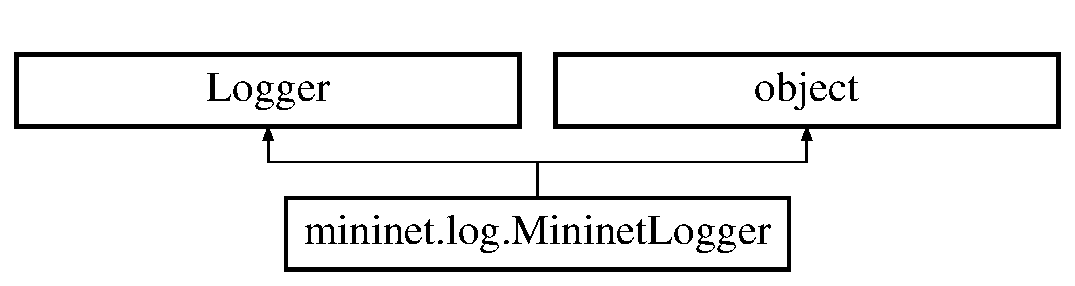
\includegraphics[height=2.000000cm]{classmininet_1_1log_1_1MininetLogger}
\end{center}
\end{figure}
\subsection*{Public Member Functions}
\begin{DoxyCompactItemize}
\item 
\hypertarget{classmininet_1_1log_1_1MininetLogger_a1f8cb5552a11a4694512e59d2b7834a7}{def {\bfseries \-\_\-\-\_\-init\-\_\-\-\_\-}}\label{classmininet_1_1log_1_1MininetLogger_a1f8cb5552a11a4694512e59d2b7834a7}

\item 
def \hyperlink{classmininet_1_1log_1_1MininetLogger_a5e32991d6a5bc1f11da8ef46a178bc9d}{set\-Log\-Level}
\item 
def \hyperlink{classmininet_1_1log_1_1MininetLogger_a2b0c766815f087c2b2462755e5174a72}{output}
\end{DoxyCompactItemize}


\subsection{Detailed Description}
\begin{DoxyVerb}Mininet-specific logger
   Enable each mininet .py file to with one import:

   from mininet.log import [lg, info, error]

   ...get a default logger that doesn't require one newline per logging
   call.

   Inherit from object to ensure that we have at least one new-style base
   class, and can then use the __metaclass__ directive, to prevent this
   error:

   TypeError: Error when calling the metaclass bases
   a new-style class can't have only classic bases

   If Python2.5/logging/__init__.py defined Filterer as a new-style class,
   via Filterer( object ): rather than Filterer, we wouldn't need this.

   Use singleton pattern to ensure only one logger is ever created.\end{DoxyVerb}
 

\subsection{Member Function Documentation}
\hypertarget{classmininet_1_1log_1_1MininetLogger_a2b0c766815f087c2b2462755e5174a72}{\index{mininet\-::log\-::\-Mininet\-Logger@{mininet\-::log\-::\-Mininet\-Logger}!output@{output}}
\index{output@{output}!mininet::log::MininetLogger@{mininet\-::log\-::\-Mininet\-Logger}}
\subsubsection[{output}]{\setlength{\rightskip}{0pt plus 5cm}def mininet.\-log.\-Mininet\-Logger.\-output (
\begin{DoxyParamCaption}
\item[{}]{self, }
\item[{}]{msg, }
\item[{}]{args, }
\item[{}]{kwargs}
\end{DoxyParamCaption}
)}}\label{classmininet_1_1log_1_1MininetLogger_a2b0c766815f087c2b2462755e5174a72}
\begin{DoxyVerb}Log 'msg % args' with severity 'OUTPUT'.

   To pass exception information, use the keyword argument exc_info
   with a true value, e.g.

   logger.warning("Houston, we have a %s", "cli output", exc_info=1)
\end{DoxyVerb}
 \hypertarget{classmininet_1_1log_1_1MininetLogger_a5e32991d6a5bc1f11da8ef46a178bc9d}{\index{mininet\-::log\-::\-Mininet\-Logger@{mininet\-::log\-::\-Mininet\-Logger}!set\-Log\-Level@{set\-Log\-Level}}
\index{set\-Log\-Level@{set\-Log\-Level}!mininet::log::MininetLogger@{mininet\-::log\-::\-Mininet\-Logger}}
\subsubsection[{set\-Log\-Level}]{\setlength{\rightskip}{0pt plus 5cm}def mininet.\-log.\-Mininet\-Logger.\-set\-Log\-Level (
\begin{DoxyParamCaption}
\item[{}]{self, }
\item[{}]{levelname = {\ttfamily None}}
\end{DoxyParamCaption}
)}}\label{classmininet_1_1log_1_1MininetLogger_a5e32991d6a5bc1f11da8ef46a178bc9d}
\begin{DoxyVerb}Setup loglevel.
   Convenience function to support lowercase names.
   levelName: level name from LEVELS\end{DoxyVerb}
 

The documentation for this class was generated from the following file\-:\begin{DoxyCompactItemize}
\item 
log.\-py\end{DoxyCompactItemize}

\hypertarget{classmininet_1_1net_1_1MininetWithControlNet}{\section{mininet.\-net.\-Mininet\-With\-Control\-Net Class Reference}
\label{classmininet_1_1net_1_1MininetWithControlNet}\index{mininet.\-net.\-Mininet\-With\-Control\-Net@{mininet.\-net.\-Mininet\-With\-Control\-Net}}
}
Inheritance diagram for mininet.\-net.\-Mininet\-With\-Control\-Net\-:\begin{figure}[H]
\begin{center}
\leavevmode
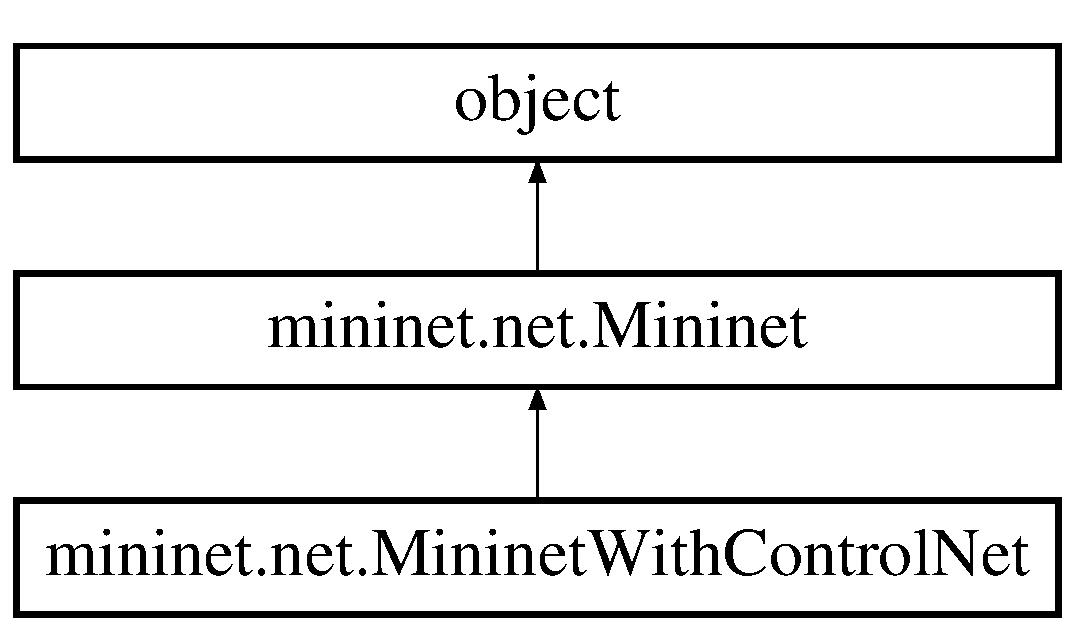
\includegraphics[height=3.000000cm]{classmininet_1_1net_1_1MininetWithControlNet}
\end{center}
\end{figure}
\subsection*{Public Member Functions}
\begin{DoxyCompactItemize}
\item 
\hypertarget{classmininet_1_1net_1_1MininetWithControlNet_ada8e763cc2bb869884a9aec47fed0a15}{def {\bfseries configure\-Control\-Network}}\label{classmininet_1_1net_1_1MininetWithControlNet_ada8e763cc2bb869884a9aec47fed0a15}

\item 
def \hyperlink{classmininet_1_1net_1_1MininetWithControlNet_a09954c5fd8df2f567db97839d2b03915}{configure\-Routed\-Control\-Network}
\end{DoxyCompactItemize}
\subsection*{Additional Inherited Members}


\subsection{Detailed Description}
\begin{DoxyVerb}Control network support:

   Create an explicit control network. Currently this is only
   used/usable with the user datapath.

   Notes:

   1. If the controller and switches are in the same (e.g. root)
      namespace, they can just use the loopback connection.

   2. If we can get unix domain sockets to work, we can use them
      instead of an explicit control network.

   3. Instead of routing, we could bridge or use 'in-band' control.

   4. Even if we dispense with this in general, it could still be
      useful for people who wish to simulate a separate control
      network (since real networks may need one!)

   5. Basically nobody ever used this code, so it has been moved
      into its own class.

   6. Ultimately we may wish to extend this to allow us to create a
      control network which every node's control interface is
      attached to.\end{DoxyVerb}
 

\subsection{Member Function Documentation}
\hypertarget{classmininet_1_1net_1_1MininetWithControlNet_a09954c5fd8df2f567db97839d2b03915}{\index{mininet\-::net\-::\-Mininet\-With\-Control\-Net@{mininet\-::net\-::\-Mininet\-With\-Control\-Net}!configure\-Routed\-Control\-Network@{configure\-Routed\-Control\-Network}}
\index{configure\-Routed\-Control\-Network@{configure\-Routed\-Control\-Network}!mininet::net::MininetWithControlNet@{mininet\-::net\-::\-Mininet\-With\-Control\-Net}}
\subsubsection[{configure\-Routed\-Control\-Network}]{\setlength{\rightskip}{0pt plus 5cm}def mininet.\-net.\-Mininet\-With\-Control\-Net.\-configure\-Routed\-Control\-Network (
\begin{DoxyParamCaption}
\item[{}]{self, }
\item[{}]{ip = {\ttfamily '192.168.123.1'}, }
\item[{}]{prefix\-Len = {\ttfamily 16}}
\end{DoxyParamCaption}
)}}\label{classmininet_1_1net_1_1MininetWithControlNet_a09954c5fd8df2f567db97839d2b03915}
\begin{DoxyVerb}Configure a routed control network on controller and switches.
   For use with the user datapath only right now.\end{DoxyVerb}
 

The documentation for this class was generated from the following file\-:\begin{DoxyCompactItemize}
\item 
net.\-py\end{DoxyCompactItemize}

\hypertarget{classmininet_1_1wifiMobility_1_1mobility}{\section{mininet.\-wifi\-Mobility.\-mobility Class Reference}
\label{classmininet_1_1wifiMobility_1_1mobility}\index{mininet.\-wifi\-Mobility.\-mobility@{mininet.\-wifi\-Mobility.\-mobility}}
}
Inheritance diagram for mininet.\-wifi\-Mobility.\-mobility\-:\begin{figure}[H]
\begin{center}
\leavevmode
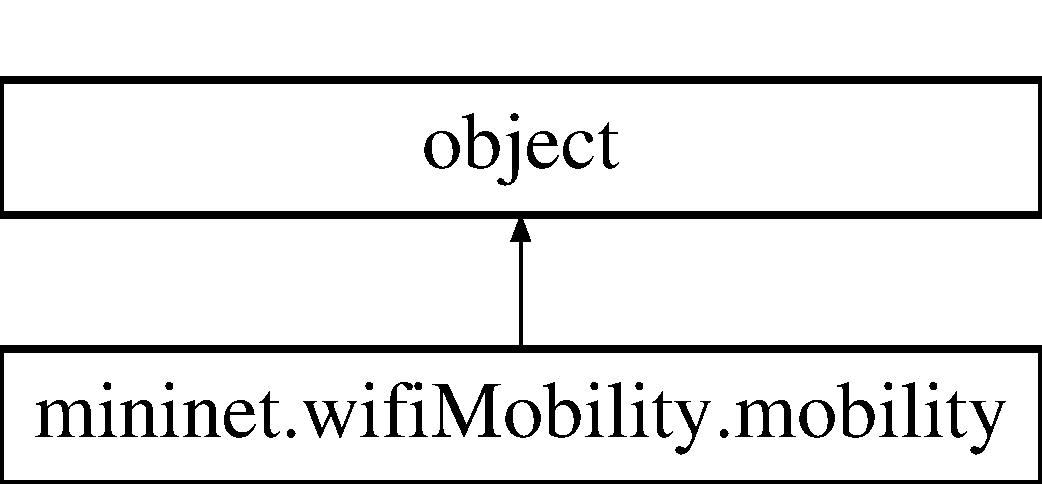
\includegraphics[height=2.000000cm]{classmininet_1_1wifiMobility_1_1mobility}
\end{center}
\end{figure}
\subsection*{Public Member Functions}
\begin{DoxyCompactItemize}
\item 
def \hyperlink{classmininet_1_1wifiMobility_1_1mobility_a7bfaf78133f30c9d812e7dd77fa836fd}{move\-Factor}
\item 
\hypertarget{classmininet_1_1wifiMobility_1_1mobility_acc7aa8b98704f410356e6d7ec4fb2be9}{def {\bfseries node\-Speed}}\label{classmininet_1_1wifiMobility_1_1mobility_acc7aa8b98704f410356e6d7ec4fb2be9}

\item 
def \hyperlink{classmininet_1_1wifiMobility_1_1mobility_a33bd8550eead3027d47320d1d4710896}{handover}
\item 
\hypertarget{classmininet_1_1wifiMobility_1_1mobility_ab1b2e7fa1a8ddcdbf0c2300a9d16e379}{def {\bfseries graph\-Instantiate\-Nodes}}\label{classmininet_1_1wifiMobility_1_1mobility_ab1b2e7fa1a8ddcdbf0c2300a9d16e379}

\item 
\hypertarget{classmininet_1_1wifiMobility_1_1mobility_a2e293ad5b68de48662ca61c151d6a088}{def {\bfseries number\-Of\-Associated\-Stations}}\label{classmininet_1_1wifiMobility_1_1mobility_a2e293ad5b68de48662ca61c151d6a088}

\item 
def \hyperlink{classmininet_1_1wifiMobility_1_1mobility_a08948c132bec721adc84746465bc76e7}{mobility\-Position\-Defined}
\item 
\hypertarget{classmininet_1_1wifiMobility_1_1mobility_a761828b57c33888c3ec79ab655dbc49b}{def {\bfseries models}}\label{classmininet_1_1wifiMobility_1_1mobility_a761828b57c33888c3ec79ab655dbc49b}

\item 
\hypertarget{classmininet_1_1wifiMobility_1_1mobility_ae958b9813f2c7c7495a50789d0c3bc0e}{def {\bfseries get\-A\-Ps\-In\-Range}}\label{classmininet_1_1wifiMobility_1_1mobility_ae958b9813f2c7c7495a50789d0c3bc0e}

\item 
\hypertarget{classmininet_1_1wifiMobility_1_1mobility_aab2327db40b2a55c84bd9af735187ceb}{def {\bfseries node\-Parameter}}\label{classmininet_1_1wifiMobility_1_1mobility_aab2327db40b2a55c84bd9af735187ceb}

\item 
\hypertarget{classmininet_1_1wifiMobility_1_1mobility_ac7413d5b666c845b2615087906d68042}{def {\bfseries parameters}}\label{classmininet_1_1wifiMobility_1_1mobility_ac7413d5b666c845b2615087906d68042}

\item 
def \hyperlink{classmininet_1_1wifiMobility_1_1mobility_af44d34258ad9306b65c1f02fae3c42e9}{set\-Channel\-Parameters}
\end{DoxyCompactItemize}
\subsection*{Public Attributes}
\begin{DoxyCompactItemize}
\item 
\hyperlink{classmininet_1_1wifiMobility_1_1mobility_a3eddb97d5e1bd75aa2fb5246204329aa}{model\-Name}
\begin{DoxyCompactList}\small\item\em Random Walk model. \end{DoxyCompactList}\end{DoxyCompactItemize}
\subsection*{Static Public Attributes}
\begin{DoxyCompactItemize}
\item 
\hypertarget{classmininet_1_1wifiMobility_1_1mobility_ae1ed852eb1114d82efec3eb0e98336e2}{int {\bfseries M\-A\-X\-\_\-\-X} = 50}\label{classmininet_1_1wifiMobility_1_1mobility_ae1ed852eb1114d82efec3eb0e98336e2}

\item 
\hypertarget{classmininet_1_1wifiMobility_1_1mobility_a98e8ab235750f1ec25a620889b4c5b25}{int {\bfseries M\-A\-X\-\_\-\-Y} = 50}\label{classmininet_1_1wifiMobility_1_1mobility_a98e8ab235750f1ec25a620889b4c5b25}

\item 
\hypertarget{classmininet_1_1wifiMobility_1_1mobility_a547ce6bfdbabbd5988a1ee83290e64fe}{dictionary {\bfseries move\-Fac} = \{\}}\label{classmininet_1_1wifiMobility_1_1mobility_a547ce6bfdbabbd5988a1ee83290e64fe}

\item 
\hypertarget{classmininet_1_1wifiMobility_1_1mobility_aee33277c7eb232cb5c6c8e09167c8623}{dictionary {\bfseries initial\-Position} = \{\}}\label{classmininet_1_1wifiMobility_1_1mobility_aee33277c7eb232cb5c6c8e09167c8623}

\item 
\hypertarget{classmininet_1_1wifiMobility_1_1mobility_a7ecc2259dd183110f644b7d46c73de1f}{dictionary {\bfseries final\-Position} = \{\}}\label{classmininet_1_1wifiMobility_1_1mobility_a7ecc2259dd183110f644b7d46c73de1f}

\item 
\hypertarget{classmininet_1_1wifiMobility_1_1mobility_a96b440e9c70a5f5b5e07e0fd2cd3fd7d}{{\bfseries association\-Control\-Method} = False}\label{classmininet_1_1wifiMobility_1_1mobility_a96b440e9c70a5f5b5e07e0fd2cd3fd7d}

\item 
\hypertarget{classmininet_1_1wifiMobility_1_1mobility_a4f56b506697addbc5e0eff5d20c8d257}{list {\bfseries ap\-List} = \mbox{[}$\,$\mbox{]}}\label{classmininet_1_1wifiMobility_1_1mobility_a4f56b506697addbc5e0eff5d20c8d257}

\item 
\hypertarget{classmininet_1_1wifiMobility_1_1mobility_a84bb1ccb14ea4b3ebc7297285226cb3b}{list {\bfseries sta\-List} = \mbox{[}$\,$\mbox{]}}\label{classmininet_1_1wifiMobility_1_1mobility_a84bb1ccb14ea4b3ebc7297285226cb3b}

\item 
\hypertarget{classmininet_1_1wifiMobility_1_1mobility_a966896c86758a729f99f32981ed4f0af}{{\bfseries D\-R\-A\-W} = False}\label{classmininet_1_1wifiMobility_1_1mobility_a966896c86758a729f99f32981ed4f0af}

\item 
\hypertarget{classmininet_1_1wifiMobility_1_1mobility_a91f4541922a12701bccc46d38b68c4b5}{{\bfseries continue\-\_\-} = True}\label{classmininet_1_1wifiMobility_1_1mobility_a91f4541922a12701bccc46d38b68c4b5}

\end{DoxyCompactItemize}


\subsection{Detailed Description}
\begin{DoxyVerb}Mobility \end{DoxyVerb}
 

\subsection{Member Function Documentation}
\hypertarget{classmininet_1_1wifiMobility_1_1mobility_a33bd8550eead3027d47320d1d4710896}{\index{mininet\-::wifi\-Mobility\-::mobility@{mininet\-::wifi\-Mobility\-::mobility}!handover@{handover}}
\index{handover@{handover}!mininet::wifiMobility::mobility@{mininet\-::wifi\-Mobility\-::mobility}}
\subsubsection[{handover}]{\setlength{\rightskip}{0pt plus 5cm}def mininet.\-wifi\-Mobility.\-mobility.\-handover (
\begin{DoxyParamCaption}
\item[{}]{self, }
\item[{}]{sta, }
\item[{}]{ap, }
\item[{}]{wlan, }
\item[{}]{distance, }
\item[{}]{change\-A\-P, }
\item[{}]{ac = {\ttfamily None}, }
\item[{}]{params}
\end{DoxyParamCaption}
)}}\label{classmininet_1_1wifiMobility_1_1mobility_a33bd8550eead3027d47320d1d4710896}
\begin{DoxyVerb}handover\end{DoxyVerb}
 \hypertarget{classmininet_1_1wifiMobility_1_1mobility_a08948c132bec721adc84746465bc76e7}{\index{mininet\-::wifi\-Mobility\-::mobility@{mininet\-::wifi\-Mobility\-::mobility}!mobility\-Position\-Defined@{mobility\-Position\-Defined}}
\index{mobility\-Position\-Defined@{mobility\-Position\-Defined}!mininet::wifiMobility::mobility@{mininet\-::wifi\-Mobility\-::mobility}}
\subsubsection[{mobility\-Position\-Defined}]{\setlength{\rightskip}{0pt plus 5cm}def mininet.\-wifi\-Mobility.\-mobility.\-mobility\-Position\-Defined (
\begin{DoxyParamCaption}
\item[{}]{self, }
\item[{}]{initial\-\_\-time, }
\item[{}]{final\-\_\-time, }
\item[{}]{sta\-Mov}
\end{DoxyParamCaption}
)}}\label{classmininet_1_1wifiMobility_1_1mobility_a08948c132bec721adc84746465bc76e7}
\begin{DoxyVerb}ongoing Mobility \end{DoxyVerb}
 \hypertarget{classmininet_1_1wifiMobility_1_1mobility_a7bfaf78133f30c9d812e7dd77fa836fd}{\index{mininet\-::wifi\-Mobility\-::mobility@{mininet\-::wifi\-Mobility\-::mobility}!move\-Factor@{move\-Factor}}
\index{move\-Factor@{move\-Factor}!mininet::wifiMobility::mobility@{mininet\-::wifi\-Mobility\-::mobility}}
\subsubsection[{move\-Factor}]{\setlength{\rightskip}{0pt plus 5cm}def mininet.\-wifi\-Mobility.\-mobility.\-move\-Factor (
\begin{DoxyParamCaption}
\item[{}]{self, }
\item[{}]{sta, }
\item[{}]{diff\-Time, }
\item[{}]{initial\-Position, }
\item[{}]{final\-Position}
\end{DoxyParamCaption}
)}}\label{classmininet_1_1wifiMobility_1_1mobility_a7bfaf78133f30c9d812e7dd77fa836fd}
\begin{DoxyVerb}    Moving nodes
    diffTime: important to calculate the speed  
\end{DoxyVerb}
 \hypertarget{classmininet_1_1wifiMobility_1_1mobility_af44d34258ad9306b65c1f02fae3c42e9}{\index{mininet\-::wifi\-Mobility\-::mobility@{mininet\-::wifi\-Mobility\-::mobility}!set\-Channel\-Parameters@{set\-Channel\-Parameters}}
\index{set\-Channel\-Parameters@{set\-Channel\-Parameters}!mininet::wifiMobility::mobility@{mininet\-::wifi\-Mobility\-::mobility}}
\subsubsection[{set\-Channel\-Parameters}]{\setlength{\rightskip}{0pt plus 5cm}def mininet.\-wifi\-Mobility.\-mobility.\-set\-Channel\-Parameters (
\begin{DoxyParamCaption}
\item[{}]{self, }
\item[{}]{sta, }
\item[{}]{ap, }
\item[{}]{dist, }
\item[{}]{wlan}
\end{DoxyParamCaption}
)}}\label{classmininet_1_1wifiMobility_1_1mobility_af44d34258ad9306b65c1f02fae3c42e9}
\begin{DoxyVerb}Wifi Parameters \end{DoxyVerb}
 

\subsection{Member Data Documentation}
\hypertarget{classmininet_1_1wifiMobility_1_1mobility_a3eddb97d5e1bd75aa2fb5246204329aa}{\index{mininet\-::wifi\-Mobility\-::mobility@{mininet\-::wifi\-Mobility\-::mobility}!model\-Name@{model\-Name}}
\index{model\-Name@{model\-Name}!mininet::wifiMobility::mobility@{mininet\-::wifi\-Mobility\-::mobility}}
\subsubsection[{model\-Name}]{\setlength{\rightskip}{0pt plus 5cm}mininet.\-wifi\-Mobility.\-mobility.\-model\-Name}}\label{classmininet_1_1wifiMobility_1_1mobility_a3eddb97d5e1bd75aa2fb5246204329aa}


Random Walk model. 

Reference Point Group model.

Gauss-\/\-Markov model.

Random Waypoint model.

Random Direction model.

Truncated Levy Walk model. 

The documentation for this class was generated from the following file\-:\begin{DoxyCompactItemize}
\item 
wifi\-Mobility.\-py\end{DoxyCompactItemize}

\hypertarget{classmininet_1_1wifiModule_1_1module}{\section{mininet.\-wifi\-Module.\-module Class Reference}
\label{classmininet_1_1wifiModule_1_1module}\index{mininet.\-wifi\-Module.\-module@{mininet.\-wifi\-Module.\-module}}
}
Inheritance diagram for mininet.\-wifi\-Module.\-module\-:\begin{figure}[H]
\begin{center}
\leavevmode
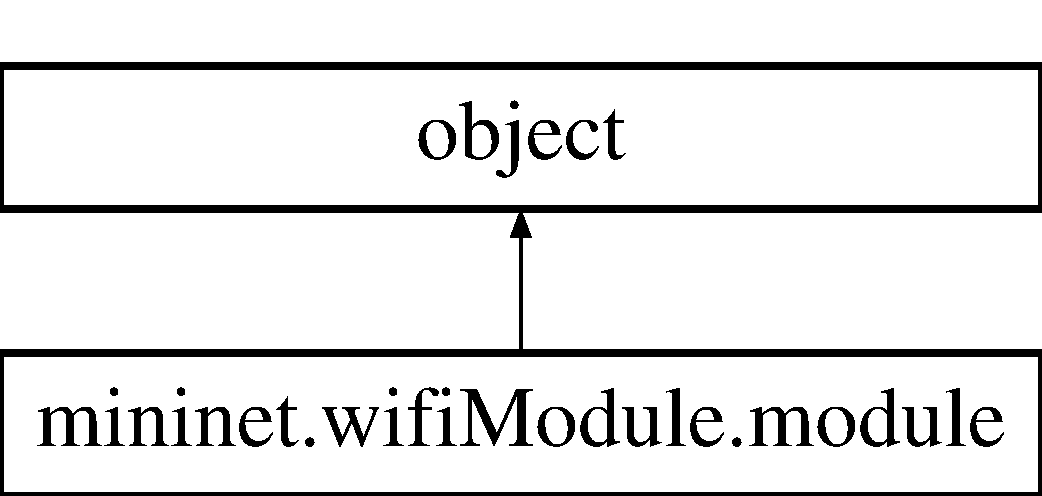
\includegraphics[height=2.000000cm]{classmininet_1_1wifiModule_1_1module}
\end{center}
\end{figure}
\subsection*{Public Member Functions}
\begin{DoxyCompactItemize}
\item 
def \hyperlink{classmininet_1_1wifiModule_1_1module_a8527224db26b4f2989c6189b075c1ce2}{load\-Module}
\item 
def \hyperlink{classmininet_1_1wifiModule_1_1module_a5a41a72e43608d1f7b640ae00ec3ccb2}{stop}
\item 
def \hyperlink{classmininet_1_1wifiModule_1_1module_ae18ef94aaf7c1e39f6e705003bf83750}{start}
\item 
\hypertarget{classmininet_1_1wifiModule_1_1module_a8a567417de222467a84c82d6bddcf022}{def {\bfseries get\-Wlan\-List}}\label{classmininet_1_1wifiModule_1_1module_a8a567417de222467a84c82d6bddcf022}

\item 
def \hyperlink{classmininet_1_1wifiModule_1_1module_af918ffcb56b56971d4689c9b0c78da6f}{get\-Phy}
\item 
\hypertarget{classmininet_1_1wifiModule_1_1module_ab7647591683f5969374a5ac4e1600324}{def {\bfseries assing\-Iface}}\label{classmininet_1_1wifiModule_1_1module_ab7647591683f5969374a5ac4e1600324}

\item 
\hypertarget{classmininet_1_1wifiModule_1_1module_ac454d404cd974bb420f7bc04711700c2}{def {\bfseries get\-Wlan\-Iface}}\label{classmininet_1_1wifiModule_1_1module_ac454d404cd974bb420f7bc04711700c2}

\end{DoxyCompactItemize}
\subsection*{Public Attributes}
\begin{DoxyCompactItemize}
\item 
\hypertarget{classmininet_1_1wifiModule_1_1module_a0bd0f08ed47a7e377717cc8944b59691}{{\bfseries wlans}}\label{classmininet_1_1wifiModule_1_1module_a0bd0f08ed47a7e377717cc8944b59691}

\item 
\hypertarget{classmininet_1_1wifiModule_1_1module_a96348e28c30ec61886895764ff842834}{{\bfseries newapif}}\label{classmininet_1_1wifiModule_1_1module_a96348e28c30ec61886895764ff842834}

\item 
\hypertarget{classmininet_1_1wifiModule_1_1module_ae09756834a8b766ad1feec8673014e92}{{\bfseries apif}}\label{classmininet_1_1wifiModule_1_1module_ae09756834a8b766ad1feec8673014e92}

\end{DoxyCompactItemize}


\subsection{Detailed Description}
\begin{DoxyVerb}Start and Stop mac80211_hwsim module \end{DoxyVerb}
 

\subsection{Member Function Documentation}
\hypertarget{classmininet_1_1wifiModule_1_1module_af918ffcb56b56971d4689c9b0c78da6f}{\index{mininet\-::wifi\-Module\-::module@{mininet\-::wifi\-Module\-::module}!get\-Phy@{get\-Phy}}
\index{get\-Phy@{get\-Phy}!mininet::wifiModule::module@{mininet\-::wifi\-Module\-::module}}
\subsubsection[{get\-Phy}]{\setlength{\rightskip}{0pt plus 5cm}def mininet.\-wifi\-Module.\-module.\-get\-Phy (
\begin{DoxyParamCaption}
\item[{}]{self}
\end{DoxyParamCaption}
)}}\label{classmininet_1_1wifiModule_1_1module_af918ffcb56b56971d4689c9b0c78da6f}
\begin{DoxyVerb}Get phy \end{DoxyVerb}
 \hypertarget{classmininet_1_1wifiModule_1_1module_a8527224db26b4f2989c6189b075c1ce2}{\index{mininet\-::wifi\-Module\-::module@{mininet\-::wifi\-Module\-::module}!load\-Module@{load\-Module}}
\index{load\-Module@{load\-Module}!mininet::wifiModule::module@{mininet\-::wifi\-Module\-::module}}
\subsubsection[{load\-Module}]{\setlength{\rightskip}{0pt plus 5cm}def mininet.\-wifi\-Module.\-module.\-load\-Module (
\begin{DoxyParamCaption}
\item[{}]{self, }
\item[{}]{wifi\-Radios}
\end{DoxyParamCaption}
)}}\label{classmininet_1_1wifiModule_1_1module_a8527224db26b4f2989c6189b075c1ce2}
\begin{DoxyVerb}Start wireless Module \end{DoxyVerb}
 \hypertarget{classmininet_1_1wifiModule_1_1module_ae18ef94aaf7c1e39f6e705003bf83750}{\index{mininet\-::wifi\-Module\-::module@{mininet\-::wifi\-Module\-::module}!start@{start}}
\index{start@{start}!mininet::wifiModule::module@{mininet\-::wifi\-Module\-::module}}
\subsubsection[{start}]{\setlength{\rightskip}{0pt plus 5cm}def mininet.\-wifi\-Module.\-module.\-start (
\begin{DoxyParamCaption}
\item[{}]{self, }
\item[{}]{wifi\-Radios}
\end{DoxyParamCaption}
)}}\label{classmininet_1_1wifiModule_1_1module_ae18ef94aaf7c1e39f6e705003bf83750}
\begin{DoxyVerb}Starting environment\end{DoxyVerb}
 \hypertarget{classmininet_1_1wifiModule_1_1module_a5a41a72e43608d1f7b640ae00ec3ccb2}{\index{mininet\-::wifi\-Module\-::module@{mininet\-::wifi\-Module\-::module}!stop@{stop}}
\index{stop@{stop}!mininet::wifiModule::module@{mininet\-::wifi\-Module\-::module}}
\subsubsection[{stop}]{\setlength{\rightskip}{0pt plus 5cm}def mininet.\-wifi\-Module.\-module.\-stop (
\begin{DoxyParamCaption}
\item[{}]{self}
\end{DoxyParamCaption}
)}}\label{classmininet_1_1wifiModule_1_1module_a5a41a72e43608d1f7b640ae00ec3ccb2}
\begin{DoxyVerb}Stop wireless Module \end{DoxyVerb}
 

The documentation for this class was generated from the following file\-:\begin{DoxyCompactItemize}
\item 
wifi\-Module.\-py\end{DoxyCompactItemize}

\hypertarget{classmininet_1_1topo_1_1MultiGraph}{\section{mininet.\-topo.\-Multi\-Graph Class Reference}
\label{classmininet_1_1topo_1_1MultiGraph}\index{mininet.\-topo.\-Multi\-Graph@{mininet.\-topo.\-Multi\-Graph}}
}
Inheritance diagram for mininet.\-topo.\-Multi\-Graph\-:\begin{figure}[H]
\begin{center}
\leavevmode
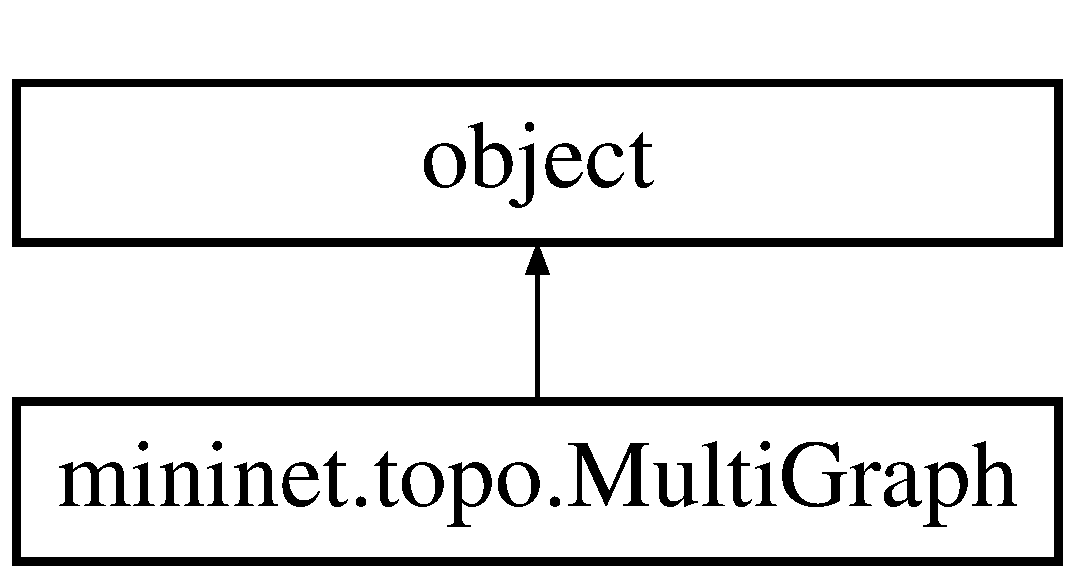
\includegraphics[height=2.000000cm]{classmininet_1_1topo_1_1MultiGraph}
\end{center}
\end{figure}
\subsection*{Public Member Functions}
\begin{DoxyCompactItemize}
\item 
\hypertarget{classmininet_1_1topo_1_1MultiGraph_aadc9c2b3464672e4a645b4aa2baeede0}{def {\bfseries \-\_\-\-\_\-init\-\_\-\-\_\-}}\label{classmininet_1_1topo_1_1MultiGraph_aadc9c2b3464672e4a645b4aa2baeede0}

\item 
def \hyperlink{classmininet_1_1topo_1_1MultiGraph_afbaa3122caa0148f45a99dc199bba3e8}{add\-\_\-node}
\item 
def \hyperlink{classmininet_1_1topo_1_1MultiGraph_a4709b637e8eb49a7d16894a615cb0129}{add\-\_\-edge}
\item 
def \hyperlink{classmininet_1_1topo_1_1MultiGraph_ac87c6d8fe2b8213484e9c86791843cf4}{nodes}
\item 
\hypertarget{classmininet_1_1topo_1_1MultiGraph_a2edec6526901fa4dc66cee1efc146ba6}{def {\bfseries edges\-\_\-iter}}\label{classmininet_1_1topo_1_1MultiGraph_a2edec6526901fa4dc66cee1efc146ba6}

\item 
\hypertarget{classmininet_1_1topo_1_1MultiGraph_a8ebae724fa85f50caf938db7f36eaba4}{def {\bfseries edges}}\label{classmininet_1_1topo_1_1MultiGraph_a8ebae724fa85f50caf938db7f36eaba4}

\item 
\hypertarget{classmininet_1_1topo_1_1MultiGraph_a527684d708c425c0d5db27cec6ebd2cc}{def {\bfseries \-\_\-\-\_\-getitem\-\_\-\-\_\-}}\label{classmininet_1_1topo_1_1MultiGraph_a527684d708c425c0d5db27cec6ebd2cc}

\item 
\hypertarget{classmininet_1_1topo_1_1MultiGraph_a55b96e0731c2809312749dc2ae0830a5}{def {\bfseries \-\_\-\-\_\-len\-\_\-\-\_\-}}\label{classmininet_1_1topo_1_1MultiGraph_a55b96e0731c2809312749dc2ae0830a5}

\item 
def \hyperlink{classmininet_1_1topo_1_1MultiGraph_a7525c22db1e71ea973d5546669d4e56c}{convert\-To}
\end{DoxyCompactItemize}
\subsection*{Public Attributes}
\begin{DoxyCompactItemize}
\item 
\hypertarget{classmininet_1_1topo_1_1MultiGraph_af84bae8fbcb84fbfd44b9ee5a5d60d0e}{{\bfseries node}}\label{classmininet_1_1topo_1_1MultiGraph_af84bae8fbcb84fbfd44b9ee5a5d60d0e}

\item 
\hypertarget{classmininet_1_1topo_1_1MultiGraph_aa812dcfb94ed8036b121b2e3f73ee33f}{{\bfseries edge}}\label{classmininet_1_1topo_1_1MultiGraph_aa812dcfb94ed8036b121b2e3f73ee33f}

\end{DoxyCompactItemize}


\subsection{Member Function Documentation}
\hypertarget{classmininet_1_1topo_1_1MultiGraph_a4709b637e8eb49a7d16894a615cb0129}{\index{mininet\-::topo\-::\-Multi\-Graph@{mininet\-::topo\-::\-Multi\-Graph}!add\-\_\-edge@{add\-\_\-edge}}
\index{add\-\_\-edge@{add\-\_\-edge}!mininet::topo::MultiGraph@{mininet\-::topo\-::\-Multi\-Graph}}
\subsubsection[{add\-\_\-edge}]{\setlength{\rightskip}{0pt plus 5cm}def mininet.\-topo.\-Multi\-Graph.\-add\-\_\-edge (
\begin{DoxyParamCaption}
\item[{}]{self, }
\item[{}]{src, }
\item[{}]{dst, }
\item[{}]{key = {\ttfamily None}, }
\item[{}]{attr\-\_\-dict = {\ttfamily None}, }
\item[{}]{attrs}
\end{DoxyParamCaption}
)}}\label{classmininet_1_1topo_1_1MultiGraph_a4709b637e8eb49a7d16894a615cb0129}
\begin{DoxyVerb}Add edge to graph
   key: optional key
   attr_dict: optional attribute dict
   attrs: more attributes
   warning: udpates attr_dict with attrs\end{DoxyVerb}
 \hypertarget{classmininet_1_1topo_1_1MultiGraph_afbaa3122caa0148f45a99dc199bba3e8}{\index{mininet\-::topo\-::\-Multi\-Graph@{mininet\-::topo\-::\-Multi\-Graph}!add\-\_\-node@{add\-\_\-node}}
\index{add\-\_\-node@{add\-\_\-node}!mininet::topo::MultiGraph@{mininet\-::topo\-::\-Multi\-Graph}}
\subsubsection[{add\-\_\-node}]{\setlength{\rightskip}{0pt plus 5cm}def mininet.\-topo.\-Multi\-Graph.\-add\-\_\-node (
\begin{DoxyParamCaption}
\item[{}]{self, }
\item[{}]{node, }
\item[{}]{attr\-\_\-dict = {\ttfamily None}, }
\item[{}]{attrs}
\end{DoxyParamCaption}
)}}\label{classmininet_1_1topo_1_1MultiGraph_afbaa3122caa0148f45a99dc199bba3e8}
\begin{DoxyVerb}Add node to graph
   attr_dict: attribute dict (optional)
   attrs: more attributes (optional)
   warning: updates attr_dict with attrs\end{DoxyVerb}
 \hypertarget{classmininet_1_1topo_1_1MultiGraph_a7525c22db1e71ea973d5546669d4e56c}{\index{mininet\-::topo\-::\-Multi\-Graph@{mininet\-::topo\-::\-Multi\-Graph}!convert\-To@{convert\-To}}
\index{convert\-To@{convert\-To}!mininet::topo::MultiGraph@{mininet\-::topo\-::\-Multi\-Graph}}
\subsubsection[{convert\-To}]{\setlength{\rightskip}{0pt plus 5cm}def mininet.\-topo.\-Multi\-Graph.\-convert\-To (
\begin{DoxyParamCaption}
\item[{}]{self, }
\item[{}]{cls, }
\item[{}]{data = {\ttfamily False}, }
\item[{}]{keys = {\ttfamily False}}
\end{DoxyParamCaption}
)}}\label{classmininet_1_1topo_1_1MultiGraph_a7525c22db1e71ea973d5546669d4e56c}
\begin{DoxyVerb}Convert to a new object of networkx.MultiGraph-like class cls
   data: include node and edge data
   keys: include edge keys as well as edge data\end{DoxyVerb}
 \hypertarget{classmininet_1_1topo_1_1MultiGraph_ac87c6d8fe2b8213484e9c86791843cf4}{\index{mininet\-::topo\-::\-Multi\-Graph@{mininet\-::topo\-::\-Multi\-Graph}!nodes@{nodes}}
\index{nodes@{nodes}!mininet::topo::MultiGraph@{mininet\-::topo\-::\-Multi\-Graph}}
\subsubsection[{nodes}]{\setlength{\rightskip}{0pt plus 5cm}def mininet.\-topo.\-Multi\-Graph.\-nodes (
\begin{DoxyParamCaption}
\item[{}]{self, }
\item[{}]{data = {\ttfamily False}}
\end{DoxyParamCaption}
)}}\label{classmininet_1_1topo_1_1MultiGraph_ac87c6d8fe2b8213484e9c86791843cf4}
\begin{DoxyVerb}Return list of graph nodes
   data: return list of ( node, attrs)\end{DoxyVerb}
 

The documentation for this class was generated from the following file\-:\begin{DoxyCompactItemize}
\item 
topo.\-py\end{DoxyCompactItemize}

\hypertarget{classmininet_1_1nodelib_1_1NAT}{\section{mininet.\-nodelib.\-N\-A\-T Class Reference}
\label{classmininet_1_1nodelib_1_1NAT}\index{mininet.\-nodelib.\-N\-A\-T@{mininet.\-nodelib.\-N\-A\-T}}
}
Inheritance diagram for mininet.\-nodelib.\-N\-A\-T\-:\begin{figure}[H]
\begin{center}
\leavevmode
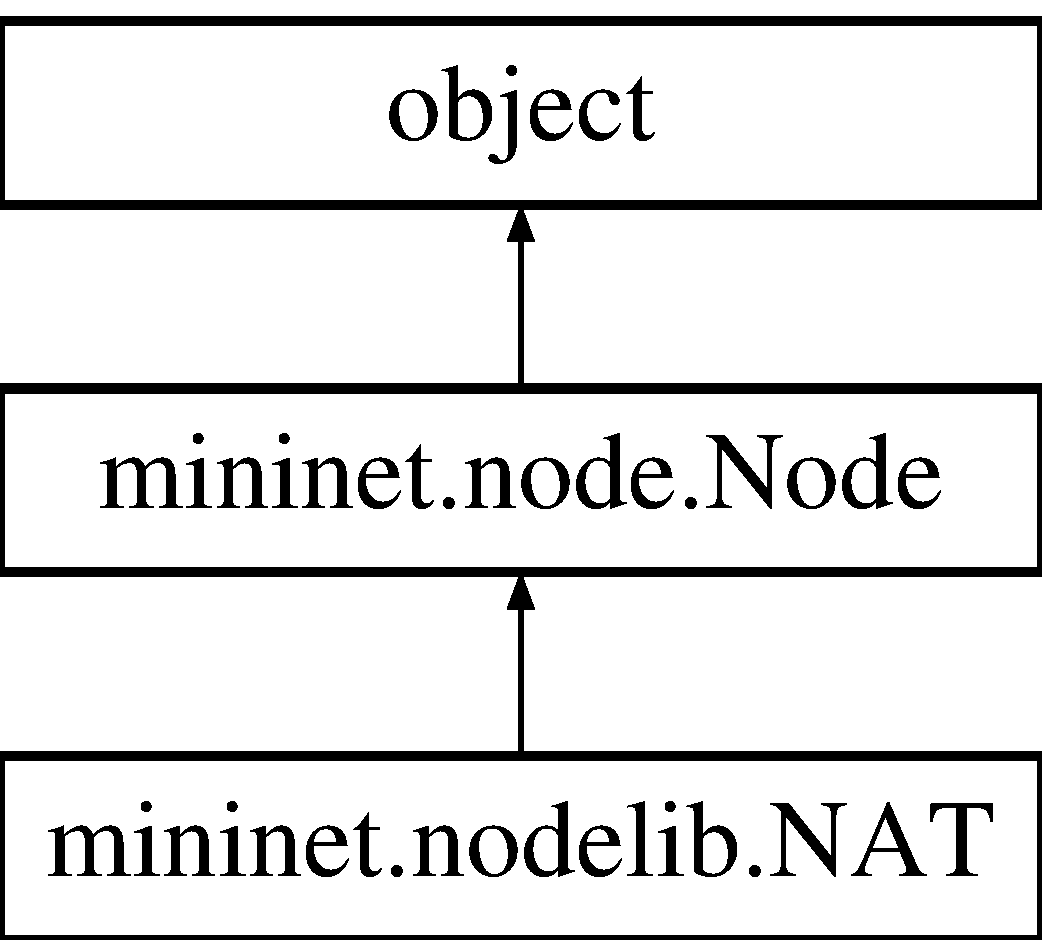
\includegraphics[height=3.000000cm]{classmininet_1_1nodelib_1_1NAT}
\end{center}
\end{figure}
\subsection*{Public Member Functions}
\begin{DoxyCompactItemize}
\item 
def \hyperlink{classmininet_1_1nodelib_1_1NAT_a54c64c441f6253d5052cf861eada67c7}{\-\_\-\-\_\-init\-\_\-\-\_\-}
\item 
def \hyperlink{classmininet_1_1nodelib_1_1NAT_a41b8cdfa25ae1333e98de36c9915075c}{config}
\item 
def \hyperlink{classmininet_1_1nodelib_1_1NAT_a13f8384350ff0d73902a5ed5c520a753}{get\-Gateway\-Intf}
\item 
def \hyperlink{classmininet_1_1nodelib_1_1NAT_ad5c247f368c06be11a87cc2ea8e5db82}{terminate}
\end{DoxyCompactItemize}
\subsection*{Public Attributes}
\begin{DoxyCompactItemize}
\item 
\hypertarget{classmininet_1_1nodelib_1_1NAT_af76b2d3545f5f0a3ede7534ba6a2d375}{{\bfseries inet\-Intf}}\label{classmininet_1_1nodelib_1_1NAT_af76b2d3545f5f0a3ede7534ba6a2d375}

\item 
\hypertarget{classmininet_1_1nodelib_1_1NAT_a66367861e1d6099e8ffabb2bcae0dda7}{{\bfseries subnet}}\label{classmininet_1_1nodelib_1_1NAT_a66367861e1d6099e8ffabb2bcae0dda7}

\item 
\hypertarget{classmininet_1_1nodelib_1_1NAT_a648889495d4ab3f64240cda2b1a8002d}{{\bfseries local\-Intf}}\label{classmininet_1_1nodelib_1_1NAT_a648889495d4ab3f64240cda2b1a8002d}

\end{DoxyCompactItemize}
\subsection*{Additional Inherited Members}


\subsection{Constructor \& Destructor Documentation}
\hypertarget{classmininet_1_1nodelib_1_1NAT_a54c64c441f6253d5052cf861eada67c7}{\index{mininet\-::nodelib\-::\-N\-A\-T@{mininet\-::nodelib\-::\-N\-A\-T}!\-\_\-\-\_\-init\-\_\-\-\_\-@{\-\_\-\-\_\-init\-\_\-\-\_\-}}
\index{\-\_\-\-\_\-init\-\_\-\-\_\-@{\-\_\-\-\_\-init\-\_\-\-\_\-}!mininet::nodelib::NAT@{mininet\-::nodelib\-::\-N\-A\-T}}
\subsubsection[{\-\_\-\-\_\-init\-\_\-\-\_\-}]{\setlength{\rightskip}{0pt plus 5cm}def mininet.\-nodelib.\-N\-A\-T.\-\_\-\-\_\-init\-\_\-\-\_\- (
\begin{DoxyParamCaption}
\item[{}]{self, }
\item[{}]{name, }
\item[{}]{inet\-Intf = {\ttfamily None}, }
\item[{}]{subnet = {\ttfamily '10.0/8'}, }
\item[{}]{local\-Intf = {\ttfamily None}, }
\item[{}]{params}
\end{DoxyParamCaption}
)}}\label{classmininet_1_1nodelib_1_1NAT_a54c64c441f6253d5052cf861eada67c7}
\begin{DoxyVerb}Start NAT/forwarding between Mininet and external network
   inetIntf: interface for internet access
   subnet: Mininet subnet (default 10.0/8)=\end{DoxyVerb}
 

\subsection{Member Function Documentation}
\hypertarget{classmininet_1_1nodelib_1_1NAT_a41b8cdfa25ae1333e98de36c9915075c}{\index{mininet\-::nodelib\-::\-N\-A\-T@{mininet\-::nodelib\-::\-N\-A\-T}!config@{config}}
\index{config@{config}!mininet::nodelib::NAT@{mininet\-::nodelib\-::\-N\-A\-T}}
\subsubsection[{config}]{\setlength{\rightskip}{0pt plus 5cm}def mininet.\-nodelib.\-N\-A\-T.\-config (
\begin{DoxyParamCaption}
\item[{}]{self, }
\item[{}]{params}
\end{DoxyParamCaption}
)}}\label{classmininet_1_1nodelib_1_1NAT_a41b8cdfa25ae1333e98de36c9915075c}
\begin{DoxyVerb}Configure the NAT and iptables\end{DoxyVerb}
 \hypertarget{classmininet_1_1nodelib_1_1NAT_a13f8384350ff0d73902a5ed5c520a753}{\index{mininet\-::nodelib\-::\-N\-A\-T@{mininet\-::nodelib\-::\-N\-A\-T}!get\-Gateway\-Intf@{get\-Gateway\-Intf}}
\index{get\-Gateway\-Intf@{get\-Gateway\-Intf}!mininet::nodelib::NAT@{mininet\-::nodelib\-::\-N\-A\-T}}
\subsubsection[{get\-Gateway\-Intf}]{\setlength{\rightskip}{0pt plus 5cm}def mininet.\-nodelib.\-N\-A\-T.\-get\-Gateway\-Intf (
\begin{DoxyParamCaption}
\item[{}]{self, }
\item[{}]{fallback = {\ttfamily 'eth0'}}
\end{DoxyParamCaption}
)}}\label{classmininet_1_1nodelib_1_1NAT_a13f8384350ff0d73902a5ed5c520a753}
\begin{DoxyVerb}Return gateway interface name
   fallback: default device to fall back to\end{DoxyVerb}
 \hypertarget{classmininet_1_1nodelib_1_1NAT_ad5c247f368c06be11a87cc2ea8e5db82}{\index{mininet\-::nodelib\-::\-N\-A\-T@{mininet\-::nodelib\-::\-N\-A\-T}!terminate@{terminate}}
\index{terminate@{terminate}!mininet::nodelib::NAT@{mininet\-::nodelib\-::\-N\-A\-T}}
\subsubsection[{terminate}]{\setlength{\rightskip}{0pt plus 5cm}def mininet.\-nodelib.\-N\-A\-T.\-terminate (
\begin{DoxyParamCaption}
\item[{}]{self}
\end{DoxyParamCaption}
)}}\label{classmininet_1_1nodelib_1_1NAT_ad5c247f368c06be11a87cc2ea8e5db82}
\begin{DoxyVerb}Stop NAT/forwarding between Mininet and external network\end{DoxyVerb}
 

The documentation for this class was generated from the following file\-:\begin{DoxyCompactItemize}
\item 
nodelib.\-py\end{DoxyCompactItemize}

\hypertarget{classmininet_1_1node_1_1Node}{\section{mininet.\-node.\-Node Class Reference}
\label{classmininet_1_1node_1_1Node}\index{mininet.\-node.\-Node@{mininet.\-node.\-Node}}
}
Inheritance diagram for mininet.\-node.\-Node\-:\begin{figure}[H]
\begin{center}
\leavevmode
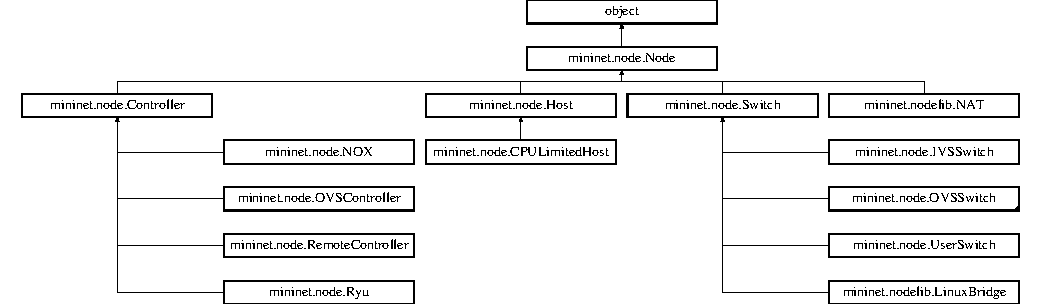
\includegraphics[height=4.083333cm]{classmininet_1_1node_1_1Node}
\end{center}
\end{figure}
\subsection*{Public Member Functions}
\begin{DoxyCompactItemize}
\item 
def \hyperlink{classmininet_1_1node_1_1Node_ae565010f2b329ac47a215ff588c483d7}{\-\_\-\-\_\-init\-\_\-\-\_\-}
\item 
def \hyperlink{classmininet_1_1node_1_1Node_ada863d2ab5219890fa1b434c7c8b90fe}{fd\-To\-Node}
\item 
\hypertarget{classmininet_1_1node_1_1Node_a69d6e6cad45d1384c16dae11e955c4b0}{def {\bfseries start\-Shell}}\label{classmininet_1_1node_1_1Node_a69d6e6cad45d1384c16dae11e955c4b0}

\item 
\hypertarget{classmininet_1_1node_1_1Node_a74b98f8d61c2b9692a9f3bb2b8defda1}{def {\bfseries calculate\-Wi\-Fi\-Parameters}}\label{classmininet_1_1node_1_1Node_a74b98f8d61c2b9692a9f3bb2b8defda1}

\item 
\hypertarget{classmininet_1_1node_1_1Node_acc4447c65d4915ce8ee0de9a8e73fe54}{def {\bfseries verifying\-Nodes}}\label{classmininet_1_1node_1_1Node_acc4447c65d4915ce8ee0de9a8e73fe54}

\item 
\hypertarget{classmininet_1_1node_1_1Node_a55298f4081afd902b9a237a004557474}{def {\bfseries mesh\-Leave}}\label{classmininet_1_1node_1_1Node_a55298f4081afd902b9a237a004557474}

\item 
\hypertarget{classmininet_1_1node_1_1Node_a1c8c1fc2623626762ed5407ac735e95e}{def {\bfseries set\-Mac}}\label{classmininet_1_1node_1_1Node_a1c8c1fc2623626762ed5407ac735e95e}

\item 
def \hyperlink{classmininet_1_1node_1_1Node_af93cd2057518eabbcaa89f413ba8af13}{associate}
\item 
\hypertarget{classmininet_1_1node_1_1Node_a1bee3bd5ce51622b15b2b3e912f997cd}{def {\bfseries set\-Range}}\label{classmininet_1_1node_1_1Node_a1bee3bd5ce51622b15b2b3e912f997cd}

\item 
\hypertarget{classmininet_1_1node_1_1Node_afe66e20f3d474dd0ad757830dbff09fb}{def {\bfseries move\-Station\-To}}\label{classmininet_1_1node_1_1Node_afe66e20f3d474dd0ad757830dbff09fb}

\item 
\hypertarget{classmininet_1_1node_1_1Node_a0727ff588006ffb3ba0bde2a856325a5}{def {\bfseries set\-Tx\-Power}}\label{classmininet_1_1node_1_1Node_a0727ff588006ffb3ba0bde2a856325a5}

\item 
\hypertarget{classmininet_1_1node_1_1Node_a6c40132c00408113afea0825ced31023}{def {\bfseries move\-Association\-To}}\label{classmininet_1_1node_1_1Node_a6c40132c00408113afea0825ced31023}

\item 
\hypertarget{classmininet_1_1node_1_1Node_ad6323a51d34c7d9ddec779a32d426133}{def {\bfseries confirm\-Infra\-Association}}\label{classmininet_1_1node_1_1Node_ad6323a51d34c7d9ddec779a32d426133}

\item 
\hypertarget{classmininet_1_1node_1_1Node_a3941198292f39bd95907ae99badeedda}{def {\bfseries is\-Associated}}\label{classmininet_1_1node_1_1Node_a3941198292f39bd95907ae99badeedda}

\item 
\hypertarget{classmininet_1_1node_1_1Node_a2a8b5853c3d6bf4eb2da4d57ce7a2593}{def {\bfseries mount\-Private\-Dirs}}\label{classmininet_1_1node_1_1Node_a2a8b5853c3d6bf4eb2da4d57ce7a2593}

\item 
\hypertarget{classmininet_1_1node_1_1Node_a75223603d06ddb4f96d977827707bf03}{def {\bfseries unmount\-Private\-Dirs}}\label{classmininet_1_1node_1_1Node_a75223603d06ddb4f96d977827707bf03}

\item 
\hypertarget{classmininet_1_1node_1_1Node_a8ffc775712b7723800e2f4af350aa409}{def {\bfseries cleanup}}\label{classmininet_1_1node_1_1Node_a8ffc775712b7723800e2f4af350aa409}

\item 
def \hyperlink{classmininet_1_1node_1_1Node_a9942b7c3670e7b719ebd4de61e477cf7}{read}
\item 
def \hyperlink{classmininet_1_1node_1_1Node_a716534e3bbc6f3cb02dfd0f5a3595701}{readline}
\item 
def \hyperlink{classmininet_1_1node_1_1Node_a12574ef66c3d0c50780e01850e56379c}{write}
\item 
\hypertarget{classmininet_1_1node_1_1Node_aef06d92666f04fc9b942858671e95ba6}{def {\bfseries terminate}}\label{classmininet_1_1node_1_1Node_aef06d92666f04fc9b942858671e95ba6}

\item 
def \hyperlink{classmininet_1_1node_1_1Node_aeb09304c74b9ca1c46bc90408adf9e05}{stop}
\item 
def \hyperlink{classmininet_1_1node_1_1Node_a9892396423f2f7d39eb656c41871082f}{wait\-Readable}
\item 
def \hyperlink{classmininet_1_1node_1_1Node_a3ab4f25f51b31d0cdf611d5d3329385b}{send\-Cmd}
\item 
\hypertarget{classmininet_1_1node_1_1Node_a100e5bf9c593daa64ffccc0b92cfe185}{def {\bfseries send\-Int}}\label{classmininet_1_1node_1_1Node_a100e5bf9c593daa64ffccc0b92cfe185}

\item 
def \hyperlink{classmininet_1_1node_1_1Node_aedc3bee4ad8ff1ea109eeb6d8a236c33}{monitor}
\item 
def \hyperlink{classmininet_1_1node_1_1Node_a842fd08ea2347808335c6ca5d94c811d}{wait\-Output}
\item 
def \hyperlink{classmininet_1_1node_1_1Node_a8245df98acbbb893c491bfe83522b0a5}{cmd}
\item 
def \hyperlink{classmininet_1_1node_1_1Node_ac964c9781bfbad931d5789a41cf2e3db}{cmd\-Print}
\item 
def \hyperlink{classmininet_1_1node_1_1Node_ab0c41eb8e690b8dfd4d50562b15c4052}{popen}
\item 
def \hyperlink{classmininet_1_1node_1_1Node_aebadf85b49be35cba33c09a2b577d0b1}{pexec}
\item 
\hypertarget{classmininet_1_1node_1_1Node_a73c8ebdbf09612a7c759f16e5434b8ef}{def {\bfseries new\-Wlan\-Port}}\label{classmininet_1_1node_1_1Node_a73c8ebdbf09612a7c759f16e5434b8ef}

\item 
\hypertarget{classmininet_1_1node_1_1Node_a35ec07f61ed11de647072510a766760b}{def {\bfseries new\-Port}}\label{classmininet_1_1node_1_1Node_a35ec07f61ed11de647072510a766760b}

\item 
def \hyperlink{classmininet_1_1node_1_1Node_aea2dde5276bd31c54cd8646da8e1b6d2}{add\-Intf}
\item 
\hypertarget{classmininet_1_1node_1_1Node_a14c12c0e1152eb84c2d2afde0d0105b7}{def {\bfseries default\-Intf}}\label{classmininet_1_1node_1_1Node_a14c12c0e1152eb84c2d2afde0d0105b7}

\item 
def \hyperlink{classmininet_1_1node_1_1Node_ab24058cbcdc431a39f566a1bbfd2e3de}{intf}
\item 
\hypertarget{classmininet_1_1node_1_1Node_ac044e7cdccae6362aeebdec85de0880f}{def {\bfseries connections\-To}}\label{classmininet_1_1node_1_1Node_ac044e7cdccae6362aeebdec85de0880f}

\item 
def \hyperlink{classmininet_1_1node_1_1Node_a6689b04e0644eaa8a990d0892e876b75}{delete\-Intfs}
\item 
def \hyperlink{classmininet_1_1node_1_1Node_a02ec5c77136e8f5820d1845570d71d22}{set\-A\-R\-P}
\item 
def \hyperlink{classmininet_1_1node_1_1Node_affbf5bd111b015509f08d868b084e7f3}{set\-Host\-Route}
\item 
def \hyperlink{classmininet_1_1node_1_1Node_a55db3f767ae191dde786757d6ea356d2}{set\-Default\-Route}
\item 
def \hyperlink{classmininet_1_1node_1_1Node_ad8f151c58ece63e1c986c667834b7d3a}{set\-M\-A\-C}
\item 
def \hyperlink{classmininet_1_1node_1_1Node_a4f399c0b11eb6358b7b9997c612ad97a}{set\-I\-P}
\item 
\hypertarget{classmininet_1_1node_1_1Node_a4fcda365ce27e856e11575f8185724a8}{def {\bfseries I\-P}}\label{classmininet_1_1node_1_1Node_a4fcda365ce27e856e11575f8185724a8}

\item 
\hypertarget{classmininet_1_1node_1_1Node_ab37efe8e3196397c33618ac4a751f0f0}{def {\bfseries M\-A\-C}}\label{classmininet_1_1node_1_1Node_ab37efe8e3196397c33618ac4a751f0f0}

\item 
\hypertarget{classmininet_1_1node_1_1Node_aa92cf4590a3bafb3c934fc292cb4db1c}{def {\bfseries intf\-Is\-Up}}\label{classmininet_1_1node_1_1Node_aa92cf4590a3bafb3c934fc292cb4db1c}

\item 
def \hyperlink{classmininet_1_1node_1_1Node_ab291d225ab2ed03bd9d6d61e65143536}{set\-Param}
\item 
def \hyperlink{classmininet_1_1node_1_1Node_a45fc4cdaf2d2b30d4185f2bdb83067f1}{config}
\item 
\hypertarget{classmininet_1_1node_1_1Node_afc8e0ef67c130408b62961bdc6c566e8}{def {\bfseries config\-Default}}\label{classmininet_1_1node_1_1Node_afc8e0ef67c130408b62961bdc6c566e8}

\item 
def \hyperlink{classmininet_1_1node_1_1Node_a6b90e2c4c4e8330b2c210df5b1ae2027}{link\-To}
\item 
\hypertarget{classmininet_1_1node_1_1Node_a396d8db5def991c6ebd41f17a936bfcb}{def {\bfseries intf\-List}}\label{classmininet_1_1node_1_1Node_a396d8db5def991c6ebd41f17a936bfcb}

\item 
\hypertarget{classmininet_1_1node_1_1Node_ac6912fd5b71c224ff1b408a7776503d0}{def {\bfseries intf\-Names}}\label{classmininet_1_1node_1_1Node_ac6912fd5b71c224ff1b408a7776503d0}

\item 
\hypertarget{classmininet_1_1node_1_1Node_ab33bd53258dba451660ee164c39fd354}{def {\bfseries \-\_\-\-\_\-repr\-\_\-\-\_\-}}\label{classmininet_1_1node_1_1Node_ab33bd53258dba451660ee164c39fd354}

\item 
\hypertarget{classmininet_1_1node_1_1Node_a9b76ff739f99f8fbbfac5ebd61c59e1d}{def {\bfseries \-\_\-\-\_\-str\-\_\-\-\_\-}}\label{classmininet_1_1node_1_1Node_a9b76ff739f99f8fbbfac5ebd61c59e1d}

\item 
\hypertarget{classmininet_1_1node_1_1Node_a394ce6bc81ff9a3c932dd925031cc208}{def {\bfseries check\-Setup}}\label{classmininet_1_1node_1_1Node_a394ce6bc81ff9a3c932dd925031cc208}

\item 
\hypertarget{classmininet_1_1node_1_1Node_a3d2c6a295ce8ad849446e922f34a0676}{def {\bfseries setup}}\label{classmininet_1_1node_1_1Node_a3d2c6a295ce8ad849446e922f34a0676}

\end{DoxyCompactItemize}
\subsection*{Public Attributes}
\begin{DoxyCompactItemize}
\item 
\hypertarget{classmininet_1_1node_1_1Node_a9bcb08b3e528808c39f84596ccf806c8}{{\bfseries name}}\label{classmininet_1_1node_1_1Node_a9bcb08b3e528808c39f84596ccf806c8}

\item 
\hypertarget{classmininet_1_1node_1_1Node_ad66152671e401c107ca10f4ce4fe8362}{{\bfseries private\-Dirs}}\label{classmininet_1_1node_1_1Node_ad66152671e401c107ca10f4ce4fe8362}

\item 
\hypertarget{classmininet_1_1node_1_1Node_aa21c21d33a9d72e3f0be58f8d549c643}{{\bfseries in\-Namespace}}\label{classmininet_1_1node_1_1Node_aa21c21d33a9d72e3f0be58f8d549c643}

\item 
\hypertarget{classmininet_1_1node_1_1Node_a2103d92a9c485b657d519c12d02a558a}{{\bfseries params}}\label{classmininet_1_1node_1_1Node_a2103d92a9c485b657d519c12d02a558a}

\item 
\hypertarget{classmininet_1_1node_1_1Node_aeabb844f254c0c3422b0bb22a2c6e9ff}{{\bfseries intfs}}\label{classmininet_1_1node_1_1Node_aeabb844f254c0c3422b0bb22a2c6e9ff}

\item 
\hypertarget{classmininet_1_1node_1_1Node_ab9de02c5ad0de00d2283bd3b4de59473}{{\bfseries ports}}\label{classmininet_1_1node_1_1Node_ab9de02c5ad0de00d2283bd3b4de59473}

\item 
\hypertarget{classmininet_1_1node_1_1Node_ac5d26cfd750afaf72de49024018cae69}{{\bfseries wlanports}}\label{classmininet_1_1node_1_1Node_ac5d26cfd750afaf72de49024018cae69}

\item 
\hypertarget{classmininet_1_1node_1_1Node_a77901076064bfb7bfe7aec23eab28bc8}{{\bfseries name\-To\-Intf}}\label{classmininet_1_1node_1_1Node_a77901076064bfb7bfe7aec23eab28bc8}

\item 
\hypertarget{classmininet_1_1node_1_1Node_ad6ed1803263add0e1086991a4c36cb30}{{\bfseries n\-Associated\-Stations}}\label{classmininet_1_1node_1_1Node_ad6ed1803263add0e1086991a4c36cb30}

\item 
\hypertarget{classmininet_1_1node_1_1Node_aaba8bc44fa147e198b5547fdd6cd3516}{{\bfseries range}}\label{classmininet_1_1node_1_1Node_aaba8bc44fa147e198b5547fdd6cd3516}

\item 
\hypertarget{classmininet_1_1node_1_1Node_afd8641d5458c7438bf37e6fa4328f7dd}{{\bfseries ssid}}\label{classmininet_1_1node_1_1Node_afd8641d5458c7438bf37e6fa4328f7dd}

\item 
\hypertarget{classmininet_1_1node_1_1Node_a2946a00844d826562b8bd88c7abba669}{{\bfseries channel}}\label{classmininet_1_1node_1_1Node_a2946a00844d826562b8bd88c7abba669}

\item 
\hypertarget{classmininet_1_1node_1_1Node_aec6ba9e761d9abf51258f07dde04322f}{{\bfseries mode}}\label{classmininet_1_1node_1_1Node_aec6ba9e761d9abf51258f07dde04322f}

\item 
\hypertarget{classmininet_1_1node_1_1Node_a0e42fbb26afd81fd5edada5e6f9171b2}{{\bfseries passwd}}\label{classmininet_1_1node_1_1Node_a0e42fbb26afd81fd5edada5e6f9171b2}

\item 
\hypertarget{classmininet_1_1node_1_1Node_a9f3b73f3aa013a9ba35f7de7072edd77}{{\bfseries security}}\label{classmininet_1_1node_1_1Node_a9f3b73f3aa013a9ba35f7de7072edd77}

\item 
\hypertarget{classmininet_1_1node_1_1Node_ace2398d07b2d7c1dc2a93a9da9d10c2d}{{\bfseries equipment\-Model}}\label{classmininet_1_1node_1_1Node_ace2398d07b2d7c1dc2a93a9da9d10c2d}

\item 
\hypertarget{classmininet_1_1node_1_1Node_aa35d034d20391ba626a63f86b3cc9420}{{\bfseries txgain}}\label{classmininet_1_1node_1_1Node_aa35d034d20391ba626a63f86b3cc9420}

\item 
\hypertarget{classmininet_1_1node_1_1Node_ac0ea5d3ac954e5c612ff37d89cf440d4}{{\bfseries rxgain}}\label{classmininet_1_1node_1_1Node_ac0ea5d3ac954e5c612ff37d89cf440d4}

\item 
\hypertarget{classmininet_1_1node_1_1Node_afac58a75f776638fe76d769615b5c891}{{\bfseries snr}}\label{classmininet_1_1node_1_1Node_afac58a75f776638fe76d769615b5c891}

\item 
\hypertarget{classmininet_1_1node_1_1Node_a45a143421cf7b7165a9094326d40c094}{{\bfseries func}}\label{classmininet_1_1node_1_1Node_a45a143421cf7b7165a9094326d40c094}

\item 
\hypertarget{classmininet_1_1node_1_1Node_af5589d54fd7a8c729a96730e472ee041}{{\bfseries connections}}\label{classmininet_1_1node_1_1Node_af5589d54fd7a8c729a96730e472ee041}

\item 
\hypertarget{classmininet_1_1node_1_1Node_aa151b5a45063b5a0902232d97a22bc89}{{\bfseries associate}}\label{classmininet_1_1node_1_1Node_aa151b5a45063b5a0902232d97a22bc89}

\item 
\hypertarget{classmininet_1_1node_1_1Node_af59baedb941e21712177cbd340050263}{{\bfseries n\-Wlans}}\label{classmininet_1_1node_1_1Node_af59baedb941e21712177cbd340050263}

\item 
\hypertarget{classmininet_1_1node_1_1Node_a887c3444f648b259a49915e199cee2d1}{{\bfseries next\-Iface}}\label{classmininet_1_1node_1_1Node_a887c3444f648b259a49915e199cee2d1}

\item 
\hypertarget{classmininet_1_1node_1_1Node_a257b2abff99f32818c318f51d404861c}{{\bfseries associated\-Ap}}\label{classmininet_1_1node_1_1Node_a257b2abff99f32818c318f51d404861c}

\item 
\hypertarget{classmininet_1_1node_1_1Node_a12bf64152dd5faa8948f7acb7dd37370}{{\bfseries addressing\-Sta}}\label{classmininet_1_1node_1_1Node_a12bf64152dd5faa8948f7acb7dd37370}

\item 
\hypertarget{classmininet_1_1node_1_1Node_a51ef55519f54cf33a51e7b7b0cd48103}{{\bfseries bring\-Up\-Iface}}\label{classmininet_1_1node_1_1Node_a51ef55519f54cf33a51e7b7b0cd48103}

\item 
\hypertarget{classmininet_1_1node_1_1Node_a1d1a308df80178d69b33230d4674115f}{{\bfseries iface\-To\-Associate}}\label{classmininet_1_1node_1_1Node_a1d1a308df80178d69b33230d4674115f}

\item 
\hypertarget{classmininet_1_1node_1_1Node_a5a205cd43f3f4d52e03b2c0e800e9d7d}{{\bfseries frequency}}\label{classmininet_1_1node_1_1Node_a5a205cd43f3f4d52e03b2c0e800e9d7d}

\item 
\hypertarget{classmininet_1_1node_1_1Node_aeca6eda481536bdaeffcfd7399ab3a49}{{\bfseries txpower}}\label{classmininet_1_1node_1_1Node_aeca6eda481536bdaeffcfd7399ab3a49}

\item 
\hypertarget{classmininet_1_1node_1_1Node_a1ab669a480147b63f581e2b0f1f91e8f}{{\bfseries antenna\-Gain}}\label{classmininet_1_1node_1_1Node_a1ab669a480147b63f581e2b0f1f91e8f}

\item 
\hypertarget{classmininet_1_1node_1_1Node_a2d3255ba823fb92f1ed8fa294cdd1d51}{{\bfseries antenna\-Height}}\label{classmininet_1_1node_1_1Node_a2d3255ba823fb92f1ed8fa294cdd1d51}

\item 
\hypertarget{classmininet_1_1node_1_1Node_aca298caa62c8c5644ead99a91fa7adde}{{\bfseries mac}}\label{classmininet_1_1node_1_1Node_aca298caa62c8c5644ead99a91fa7adde}

\item 
\hypertarget{classmininet_1_1node_1_1Node_a0a65102e928c59c47637f84edb67a100}{{\bfseries rssi}}\label{classmininet_1_1node_1_1Node_a0a65102e928c59c47637f84edb67a100}

\item 
\hypertarget{classmininet_1_1node_1_1Node_af7bf14841f29d155cd39284a75fb641f}{{\bfseries wlan\-To\-Associate}}\label{classmininet_1_1node_1_1Node_af7bf14841f29d155cd39284a75fb641f}

\item 
\hypertarget{classmininet_1_1node_1_1Node_ada26bee2631f3fbc90d04848747ca7cb}{{\bfseries mesh\-Mac}}\label{classmininet_1_1node_1_1Node_ada26bee2631f3fbc90d04848747ca7cb}

\item 
\hypertarget{classmininet_1_1node_1_1Node_a41ec84a755dca1509a5ad1379af56dfd}{{\bfseries type}}\label{classmininet_1_1node_1_1Node_a41ec84a755dca1509a5ad1379af56dfd}

\item 
\hypertarget{classmininet_1_1node_1_1Node_a77656b39e0f84a868d2eeb00a9dcbc2f}{{\bfseries in\-Range\-A\-Ps}}\label{classmininet_1_1node_1_1Node_a77656b39e0f84a868d2eeb00a9dcbc2f}

\item 
\hypertarget{classmininet_1_1node_1_1Node_ad413b4fbcf14c7fa034f53ccb3157eaf}{{\bfseries position}}\label{classmininet_1_1node_1_1Node_ad413b4fbcf14c7fa034f53ccb3157eaf}

\item 
\hypertarget{classmininet_1_1node_1_1Node_a0f8ec06ee293e9f10bf32e93339bcaf1}{{\bfseries start\-Position}}\label{classmininet_1_1node_1_1Node_a0f8ec06ee293e9f10bf32e93339bcaf1}

\item 
\hypertarget{classmininet_1_1node_1_1Node_af4306dd2bc8edc05574094f57d78c936}{{\bfseries end\-Position}}\label{classmininet_1_1node_1_1Node_af4306dd2bc8edc05574094f57d78c936}

\item 
\hypertarget{classmininet_1_1node_1_1Node_a467741a41f496345456808e6a44b0a25}{{\bfseries move\-Sta}}\label{classmininet_1_1node_1_1Node_a467741a41f496345456808e6a44b0a25}

\item 
\hypertarget{classmininet_1_1node_1_1Node_a8b0a9c0bd662756a376b6131e904338e}{{\bfseries associated\-Stations}}\label{classmininet_1_1node_1_1Node_a8b0a9c0bd662756a376b6131e904338e}

\item 
\hypertarget{classmininet_1_1node_1_1Node_a1111496fbbb645f2e0ad0dd0e6275fce}{{\bfseries is\-Associated}}\label{classmininet_1_1node_1_1Node_a1111496fbbb645f2e0ad0dd0e6275fce}

\item 
\hypertarget{classmininet_1_1node_1_1Node_af1a9e767b795137822b19e336c58932e}{{\bfseries sta\-Associated}}\label{classmininet_1_1node_1_1Node_af1a9e767b795137822b19e336c58932e}

\item 
\hypertarget{classmininet_1_1node_1_1Node_a49daafac5a069258b36d81a560ba81e0}{{\bfseries max\-\_\-speed}}\label{classmininet_1_1node_1_1Node_a49daafac5a069258b36d81a560ba81e0}

\item 
\hypertarget{classmininet_1_1node_1_1Node_a271b4e7347660a6399f79aa3258613fd}{{\bfseries min\-\_\-speed}}\label{classmininet_1_1node_1_1Node_a271b4e7347660a6399f79aa3258613fd}

\item 
\hypertarget{classmininet_1_1node_1_1Node_a63e49a53b9f8673244d3adc338ed7711}{{\bfseries waiting}}\label{classmininet_1_1node_1_1Node_a63e49a53b9f8673244d3adc338ed7711}

\item 
\hypertarget{classmininet_1_1node_1_1Node_a7a0dfbd10f307594e3743dc21ee1f278}{{\bfseries readbuf}}\label{classmininet_1_1node_1_1Node_a7a0dfbd10f307594e3743dc21ee1f278}

\item 
\hypertarget{classmininet_1_1node_1_1Node_a083e25e0b3bc2ae787ffd3b937cc1c27}{{\bfseries shell}}\label{classmininet_1_1node_1_1Node_a083e25e0b3bc2ae787ffd3b937cc1c27}

\item 
\hypertarget{classmininet_1_1node_1_1Node_a0213d88eac57e3d1af224f66a3ab7274}{{\bfseries stdin}}\label{classmininet_1_1node_1_1Node_a0213d88eac57e3d1af224f66a3ab7274}

\item 
\hypertarget{classmininet_1_1node_1_1Node_a58b04987af2a3bf5c7eb2a6dbf12063c}{{\bfseries stdout}}\label{classmininet_1_1node_1_1Node_a58b04987af2a3bf5c7eb2a6dbf12063c}

\item 
\hypertarget{classmininet_1_1node_1_1Node_af9a48ab1679e659d1f867ccd4f030da7}{{\bfseries pid}}\label{classmininet_1_1node_1_1Node_af9a48ab1679e659d1f867ccd4f030da7}

\item 
\hypertarget{classmininet_1_1node_1_1Node_af2e6d9b5d278c9e46d369a62b39dab86}{{\bfseries poll\-Out}}\label{classmininet_1_1node_1_1Node_af2e6d9b5d278c9e46d369a62b39dab86}

\item 
\hypertarget{classmininet_1_1node_1_1Node_aaf3d6cf50da7eaa7b52c24997eca5023}{{\bfseries execed}}\label{classmininet_1_1node_1_1Node_aaf3d6cf50da7eaa7b52c24997eca5023}

\item 
\hypertarget{classmininet_1_1node_1_1Node_a2421f6657870f65e0d4e280f3966a190}{{\bfseries last\-Cmd}}\label{classmininet_1_1node_1_1Node_a2421f6657870f65e0d4e280f3966a190}

\item 
\hypertarget{classmininet_1_1node_1_1Node_a532a23b5539c023cb0dd8f92025fbaa8}{{\bfseries last\-Pid}}\label{classmininet_1_1node_1_1Node_a532a23b5539c023cb0dd8f92025fbaa8}

\end{DoxyCompactItemize}
\subsection*{Static Public Attributes}
\begin{DoxyCompactItemize}
\item 
\hypertarget{classmininet_1_1node_1_1Node_ad3ff96047551b59c030fb002e92d9ddc}{int {\bfseries port\-Base} = 0}\label{classmininet_1_1node_1_1Node_ad3ff96047551b59c030fb002e92d9ddc}

\item 
\hypertarget{classmininet_1_1node_1_1Node_a207454e6896d503346f70539b11a94bd}{int {\bfseries port\-Wlan\-Base} = 0}\label{classmininet_1_1node_1_1Node_a207454e6896d503346f70539b11a94bd}

\item 
\hypertarget{classmininet_1_1node_1_1Node_a2b2f264edd216076c8061b106175872c}{dictionary {\bfseries in\-To\-Node} = \{\}}\label{classmininet_1_1node_1_1Node_a2b2f264edd216076c8061b106175872c}

\item 
\hypertarget{classmininet_1_1node_1_1Node_a4ed3f6ef4a5955c35f4a2f5c6a327201}{dictionary {\bfseries out\-To\-Node} = \{\}}\label{classmininet_1_1node_1_1Node_a4ed3f6ef4a5955c35f4a2f5c6a327201}

\item 
\hypertarget{classmininet_1_1node_1_1Node_a336ba69db8fe753e780df804a25f391b}{{\bfseries is\-Setup} = False}\label{classmininet_1_1node_1_1Node_a336ba69db8fe753e780df804a25f391b}

\end{DoxyCompactItemize}


\subsection{Detailed Description}
\begin{DoxyVerb}A virtual network node is simply a shell in a network namespace.
   We communicate with it using pipes.\end{DoxyVerb}
 

\subsection{Constructor \& Destructor Documentation}
\hypertarget{classmininet_1_1node_1_1Node_ae565010f2b329ac47a215ff588c483d7}{\index{mininet\-::node\-::\-Node@{mininet\-::node\-::\-Node}!\-\_\-\-\_\-init\-\_\-\-\_\-@{\-\_\-\-\_\-init\-\_\-\-\_\-}}
\index{\-\_\-\-\_\-init\-\_\-\-\_\-@{\-\_\-\-\_\-init\-\_\-\-\_\-}!mininet::node::Node@{mininet\-::node\-::\-Node}}
\subsubsection[{\-\_\-\-\_\-init\-\_\-\-\_\-}]{\setlength{\rightskip}{0pt plus 5cm}def mininet.\-node.\-Node.\-\_\-\-\_\-init\-\_\-\-\_\- (
\begin{DoxyParamCaption}
\item[{}]{self, }
\item[{}]{name, }
\item[{}]{in\-Namespace = {\ttfamily True}, }
\item[{}]{params}
\end{DoxyParamCaption}
)}}\label{classmininet_1_1node_1_1Node_ae565010f2b329ac47a215ff588c483d7}
\begin{DoxyVerb}name: name of node
   inNamespace: in network namespace?
   privateDirs: list of private directory strings or tuples
   params: Node parameters (see config() for details)\end{DoxyVerb}
 

\subsection{Member Function Documentation}
\hypertarget{classmininet_1_1node_1_1Node_aea2dde5276bd31c54cd8646da8e1b6d2}{\index{mininet\-::node\-::\-Node@{mininet\-::node\-::\-Node}!add\-Intf@{add\-Intf}}
\index{add\-Intf@{add\-Intf}!mininet::node::Node@{mininet\-::node\-::\-Node}}
\subsubsection[{add\-Intf}]{\setlength{\rightskip}{0pt plus 5cm}def mininet.\-node.\-Node.\-add\-Intf (
\begin{DoxyParamCaption}
\item[{}]{self, }
\item[{}]{intf, }
\item[{}]{port = {\ttfamily None}, }
\item[{}]{move\-Intf\-Fn = {\ttfamily moveIntf}}
\end{DoxyParamCaption}
)}}\label{classmininet_1_1node_1_1Node_aea2dde5276bd31c54cd8646da8e1b6d2}
\begin{DoxyVerb}Add an interface.
   intf: interface
   port: port number (optional, typically OpenFlow port number)
   moveIntfFn: function to move interface (optional)\end{DoxyVerb}
 \hypertarget{classmininet_1_1node_1_1Node_af93cd2057518eabbcaa89f413ba8af13}{\index{mininet\-::node\-::\-Node@{mininet\-::node\-::\-Node}!associate@{associate}}
\index{associate@{associate}!mininet::node::Node@{mininet\-::node\-::\-Node}}
\subsubsection[{associate}]{\setlength{\rightskip}{0pt plus 5cm}def mininet.\-node.\-Node.\-associate (
\begin{DoxyParamCaption}
\item[{}]{self, }
\item[{}]{sta, }
\item[{}]{ap}
\end{DoxyParamCaption}
)}}\label{classmininet_1_1node_1_1Node_af93cd2057518eabbcaa89f413ba8af13}
\begin{DoxyVerb}Associate to an Access Point \end{DoxyVerb}
 \hypertarget{classmininet_1_1node_1_1Node_a8245df98acbbb893c491bfe83522b0a5}{\index{mininet\-::node\-::\-Node@{mininet\-::node\-::\-Node}!cmd@{cmd}}
\index{cmd@{cmd}!mininet::node::Node@{mininet\-::node\-::\-Node}}
\subsubsection[{cmd}]{\setlength{\rightskip}{0pt plus 5cm}def mininet.\-node.\-Node.\-cmd (
\begin{DoxyParamCaption}
\item[{}]{self, }
\item[{}]{args, }
\item[{}]{kwargs}
\end{DoxyParamCaption}
)}}\label{classmininet_1_1node_1_1Node_a8245df98acbbb893c491bfe83522b0a5}
\begin{DoxyVerb}Send a command, wait for output, and return it.
   cmd: string\end{DoxyVerb}
 \hypertarget{classmininet_1_1node_1_1Node_ac964c9781bfbad931d5789a41cf2e3db}{\index{mininet\-::node\-::\-Node@{mininet\-::node\-::\-Node}!cmd\-Print@{cmd\-Print}}
\index{cmd\-Print@{cmd\-Print}!mininet::node::Node@{mininet\-::node\-::\-Node}}
\subsubsection[{cmd\-Print}]{\setlength{\rightskip}{0pt plus 5cm}def mininet.\-node.\-Node.\-cmd\-Print (
\begin{DoxyParamCaption}
\item[{}]{self, }
\item[{}]{args}
\end{DoxyParamCaption}
)}}\label{classmininet_1_1node_1_1Node_ac964c9781bfbad931d5789a41cf2e3db}
\begin{DoxyVerb}Call cmd and printing its output
   cmd: string\end{DoxyVerb}
 \hypertarget{classmininet_1_1node_1_1Node_a45fc4cdaf2d2b30d4185f2bdb83067f1}{\index{mininet\-::node\-::\-Node@{mininet\-::node\-::\-Node}!config@{config}}
\index{config@{config}!mininet::node::Node@{mininet\-::node\-::\-Node}}
\subsubsection[{config}]{\setlength{\rightskip}{0pt plus 5cm}def mininet.\-node.\-Node.\-config (
\begin{DoxyParamCaption}
\item[{}]{self, }
\item[{}]{mac = {\ttfamily None}, }
\item[{}]{ip = {\ttfamily None}, }
\item[{}]{default\-Route = {\ttfamily None}, }
\item[{}]{lo = {\ttfamily 'up'}, }
\item[{}]{\-\_\-params}
\end{DoxyParamCaption}
)}}\label{classmininet_1_1node_1_1Node_a45fc4cdaf2d2b30d4185f2bdb83067f1}
\begin{DoxyVerb}Configure Node according to (optional) parameters:
   mac: MAC address for default interface
   ip: IP address for default interface
   ifconfig: arbitrary interface configuration
   Subclasses should override this method and call
   the parent class's config(**params)\end{DoxyVerb}
 \hypertarget{classmininet_1_1node_1_1Node_a6689b04e0644eaa8a990d0892e876b75}{\index{mininet\-::node\-::\-Node@{mininet\-::node\-::\-Node}!delete\-Intfs@{delete\-Intfs}}
\index{delete\-Intfs@{delete\-Intfs}!mininet::node::Node@{mininet\-::node\-::\-Node}}
\subsubsection[{delete\-Intfs}]{\setlength{\rightskip}{0pt plus 5cm}def mininet.\-node.\-Node.\-delete\-Intfs (
\begin{DoxyParamCaption}
\item[{}]{self, }
\item[{}]{check\-Name = {\ttfamily True}}
\end{DoxyParamCaption}
)}}\label{classmininet_1_1node_1_1Node_a6689b04e0644eaa8a990d0892e876b75}
\begin{DoxyVerb}Delete all of our interfaces.
   checkName: only delete interfaces that contain our name\end{DoxyVerb}
 \hypertarget{classmininet_1_1node_1_1Node_ada863d2ab5219890fa1b434c7c8b90fe}{\index{mininet\-::node\-::\-Node@{mininet\-::node\-::\-Node}!fd\-To\-Node@{fd\-To\-Node}}
\index{fd\-To\-Node@{fd\-To\-Node}!mininet::node::Node@{mininet\-::node\-::\-Node}}
\subsubsection[{fd\-To\-Node}]{\setlength{\rightskip}{0pt plus 5cm}def mininet.\-node.\-Node.\-fd\-To\-Node (
\begin{DoxyParamCaption}
\item[{}]{cls, }
\item[{}]{fd}
\end{DoxyParamCaption}
)}}\label{classmininet_1_1node_1_1Node_ada863d2ab5219890fa1b434c7c8b90fe}
\begin{DoxyVerb}Return node corresponding to given file descriptor.
   fd: file descriptor
   returns: node\end{DoxyVerb}
 \hypertarget{classmininet_1_1node_1_1Node_ab24058cbcdc431a39f566a1bbfd2e3de}{\index{mininet\-::node\-::\-Node@{mininet\-::node\-::\-Node}!intf@{intf}}
\index{intf@{intf}!mininet::node::Node@{mininet\-::node\-::\-Node}}
\subsubsection[{intf}]{\setlength{\rightskip}{0pt plus 5cm}def mininet.\-node.\-Node.\-intf (
\begin{DoxyParamCaption}
\item[{}]{self, }
\item[{}]{intf = {\ttfamily None}}
\end{DoxyParamCaption}
)}}\label{classmininet_1_1node_1_1Node_ab24058cbcdc431a39f566a1bbfd2e3de}
\begin{DoxyVerb}Return our interface object with given string name,
   default intf if name is falsy (None, empty string, etc).
   or the input intf arg.

Having this fcn return its arg for Intf objects makes it
easier to construct functions with flexible input args for
interfaces (those that accept both string names and Intf objects).
\end{DoxyVerb}
 \hypertarget{classmininet_1_1node_1_1Node_a6b90e2c4c4e8330b2c210df5b1ae2027}{\index{mininet\-::node\-::\-Node@{mininet\-::node\-::\-Node}!link\-To@{link\-To}}
\index{link\-To@{link\-To}!mininet::node::Node@{mininet\-::node\-::\-Node}}
\subsubsection[{link\-To}]{\setlength{\rightskip}{0pt plus 5cm}def mininet.\-node.\-Node.\-link\-To (
\begin{DoxyParamCaption}
\item[{}]{self, }
\item[{}]{node, }
\item[{}]{link = {\ttfamily {\bf Link}}}
\end{DoxyParamCaption}
)}}\label{classmininet_1_1node_1_1Node_a6b90e2c4c4e8330b2c210df5b1ae2027}
\begin{DoxyVerb}(Deprecated) Link to another node
   replace with Link( node1, node2)\end{DoxyVerb}
 \hypertarget{classmininet_1_1node_1_1Node_aedc3bee4ad8ff1ea109eeb6d8a236c33}{\index{mininet\-::node\-::\-Node@{mininet\-::node\-::\-Node}!monitor@{monitor}}
\index{monitor@{monitor}!mininet::node::Node@{mininet\-::node\-::\-Node}}
\subsubsection[{monitor}]{\setlength{\rightskip}{0pt plus 5cm}def mininet.\-node.\-Node.\-monitor (
\begin{DoxyParamCaption}
\item[{}]{self, }
\item[{}]{timeoutms = {\ttfamily None}, }
\item[{}]{find\-Pid = {\ttfamily True}}
\end{DoxyParamCaption}
)}}\label{classmininet_1_1node_1_1Node_aedc3bee4ad8ff1ea109eeb6d8a236c33}
\begin{DoxyVerb}Monitor and return the output of a command.
   Set self.waiting to False if command has completed.
   timeoutms: timeout in ms or None to wait indefinitely
   findPid: look for PID from mnexec -p\end{DoxyVerb}
 \hypertarget{classmininet_1_1node_1_1Node_aebadf85b49be35cba33c09a2b577d0b1}{\index{mininet\-::node\-::\-Node@{mininet\-::node\-::\-Node}!pexec@{pexec}}
\index{pexec@{pexec}!mininet::node::Node@{mininet\-::node\-::\-Node}}
\subsubsection[{pexec}]{\setlength{\rightskip}{0pt plus 5cm}def mininet.\-node.\-Node.\-pexec (
\begin{DoxyParamCaption}
\item[{}]{self, }
\item[{}]{args, }
\item[{}]{kwargs}
\end{DoxyParamCaption}
)}}\label{classmininet_1_1node_1_1Node_aebadf85b49be35cba33c09a2b577d0b1}
\begin{DoxyVerb}Execute a command using popen
   returns: out, err, exitcode\end{DoxyVerb}
 \hypertarget{classmininet_1_1node_1_1Node_ab0c41eb8e690b8dfd4d50562b15c4052}{\index{mininet\-::node\-::\-Node@{mininet\-::node\-::\-Node}!popen@{popen}}
\index{popen@{popen}!mininet::node::Node@{mininet\-::node\-::\-Node}}
\subsubsection[{popen}]{\setlength{\rightskip}{0pt plus 5cm}def mininet.\-node.\-Node.\-popen (
\begin{DoxyParamCaption}
\item[{}]{self, }
\item[{}]{args, }
\item[{}]{kwargs}
\end{DoxyParamCaption}
)}}\label{classmininet_1_1node_1_1Node_ab0c41eb8e690b8dfd4d50562b15c4052}
\begin{DoxyVerb}Return a Popen() object in our namespace
   args: Popen() args, single list, or string
   kwargs: Popen() keyword args\end{DoxyVerb}
 \hypertarget{classmininet_1_1node_1_1Node_a9942b7c3670e7b719ebd4de61e477cf7}{\index{mininet\-::node\-::\-Node@{mininet\-::node\-::\-Node}!read@{read}}
\index{read@{read}!mininet::node::Node@{mininet\-::node\-::\-Node}}
\subsubsection[{read}]{\setlength{\rightskip}{0pt plus 5cm}def mininet.\-node.\-Node.\-read (
\begin{DoxyParamCaption}
\item[{}]{self, }
\item[{}]{maxbytes = {\ttfamily 1024}}
\end{DoxyParamCaption}
)}}\label{classmininet_1_1node_1_1Node_a9942b7c3670e7b719ebd4de61e477cf7}
\begin{DoxyVerb}Buffered read from node, non-blocking.
   maxbytes: maximum number of bytes to return\end{DoxyVerb}
 \hypertarget{classmininet_1_1node_1_1Node_a716534e3bbc6f3cb02dfd0f5a3595701}{\index{mininet\-::node\-::\-Node@{mininet\-::node\-::\-Node}!readline@{readline}}
\index{readline@{readline}!mininet::node::Node@{mininet\-::node\-::\-Node}}
\subsubsection[{readline}]{\setlength{\rightskip}{0pt plus 5cm}def mininet.\-node.\-Node.\-readline (
\begin{DoxyParamCaption}
\item[{}]{self}
\end{DoxyParamCaption}
)}}\label{classmininet_1_1node_1_1Node_a716534e3bbc6f3cb02dfd0f5a3595701}
\begin{DoxyVerb}Buffered readline from node, non-blocking.
   returns: line (minus newline) or None\end{DoxyVerb}
 \hypertarget{classmininet_1_1node_1_1Node_a3ab4f25f51b31d0cdf611d5d3329385b}{\index{mininet\-::node\-::\-Node@{mininet\-::node\-::\-Node}!send\-Cmd@{send\-Cmd}}
\index{send\-Cmd@{send\-Cmd}!mininet::node::Node@{mininet\-::node\-::\-Node}}
\subsubsection[{send\-Cmd}]{\setlength{\rightskip}{0pt plus 5cm}def mininet.\-node.\-Node.\-send\-Cmd (
\begin{DoxyParamCaption}
\item[{}]{self, }
\item[{}]{args, }
\item[{}]{kwargs}
\end{DoxyParamCaption}
)}}\label{classmininet_1_1node_1_1Node_a3ab4f25f51b31d0cdf611d5d3329385b}
\begin{DoxyVerb}Send a command, followed by a command to echo a sentinel,
   and return without waiting for the command to complete.
   args: command and arguments, or string
   printPid: print command's PID? (False)\end{DoxyVerb}
 \hypertarget{classmininet_1_1node_1_1Node_a02ec5c77136e8f5820d1845570d71d22}{\index{mininet\-::node\-::\-Node@{mininet\-::node\-::\-Node}!set\-A\-R\-P@{set\-A\-R\-P}}
\index{set\-A\-R\-P@{set\-A\-R\-P}!mininet::node::Node@{mininet\-::node\-::\-Node}}
\subsubsection[{set\-A\-R\-P}]{\setlength{\rightskip}{0pt plus 5cm}def mininet.\-node.\-Node.\-set\-A\-R\-P (
\begin{DoxyParamCaption}
\item[{}]{self, }
\item[{}]{ip, }
\item[{}]{mac}
\end{DoxyParamCaption}
)}}\label{classmininet_1_1node_1_1Node_a02ec5c77136e8f5820d1845570d71d22}
\begin{DoxyVerb}Add an ARP entry.
   ip: IP address as string
   mac: MAC address as string\end{DoxyVerb}
 \hypertarget{classmininet_1_1node_1_1Node_a55db3f767ae191dde786757d6ea356d2}{\index{mininet\-::node\-::\-Node@{mininet\-::node\-::\-Node}!set\-Default\-Route@{set\-Default\-Route}}
\index{set\-Default\-Route@{set\-Default\-Route}!mininet::node::Node@{mininet\-::node\-::\-Node}}
\subsubsection[{set\-Default\-Route}]{\setlength{\rightskip}{0pt plus 5cm}def mininet.\-node.\-Node.\-set\-Default\-Route (
\begin{DoxyParamCaption}
\item[{}]{self, }
\item[{}]{intf = {\ttfamily None}}
\end{DoxyParamCaption}
)}}\label{classmininet_1_1node_1_1Node_a55db3f767ae191dde786757d6ea356d2}
\begin{DoxyVerb}Set the default route to go through intf.
   intf: Intf or {dev <intfname> via <gw-ip> ...}\end{DoxyVerb}
 \hypertarget{classmininet_1_1node_1_1Node_affbf5bd111b015509f08d868b084e7f3}{\index{mininet\-::node\-::\-Node@{mininet\-::node\-::\-Node}!set\-Host\-Route@{set\-Host\-Route}}
\index{set\-Host\-Route@{set\-Host\-Route}!mininet::node::Node@{mininet\-::node\-::\-Node}}
\subsubsection[{set\-Host\-Route}]{\setlength{\rightskip}{0pt plus 5cm}def mininet.\-node.\-Node.\-set\-Host\-Route (
\begin{DoxyParamCaption}
\item[{}]{self, }
\item[{}]{ip, }
\item[{}]{intf}
\end{DoxyParamCaption}
)}}\label{classmininet_1_1node_1_1Node_affbf5bd111b015509f08d868b084e7f3}
\begin{DoxyVerb}Add route to host.
   ip: IP address as dotted decimal
   intf: string, interface name\end{DoxyVerb}
 \hypertarget{classmininet_1_1node_1_1Node_a4f399c0b11eb6358b7b9997c612ad97a}{\index{mininet\-::node\-::\-Node@{mininet\-::node\-::\-Node}!set\-I\-P@{set\-I\-P}}
\index{set\-I\-P@{set\-I\-P}!mininet::node::Node@{mininet\-::node\-::\-Node}}
\subsubsection[{set\-I\-P}]{\setlength{\rightskip}{0pt plus 5cm}def mininet.\-node.\-Node.\-set\-I\-P (
\begin{DoxyParamCaption}
\item[{}]{self, }
\item[{}]{ip, }
\item[{}]{prefix\-Len = {\ttfamily 8}, }
\item[{}]{intf = {\ttfamily None}, }
\item[{}]{kwargs}
\end{DoxyParamCaption}
)}}\label{classmininet_1_1node_1_1Node_a4f399c0b11eb6358b7b9997c612ad97a}
\begin{DoxyVerb}Set the IP address for an interface.
   intf: intf or intf name
   ip: IP address as a string
   prefixLen: prefix length, e.g. 8 for /8 or 16M addrs
   kwargs: any additional arguments for intf.setIP\end{DoxyVerb}
 \hypertarget{classmininet_1_1node_1_1Node_ad8f151c58ece63e1c986c667834b7d3a}{\index{mininet\-::node\-::\-Node@{mininet\-::node\-::\-Node}!set\-M\-A\-C@{set\-M\-A\-C}}
\index{set\-M\-A\-C@{set\-M\-A\-C}!mininet::node::Node@{mininet\-::node\-::\-Node}}
\subsubsection[{set\-M\-A\-C}]{\setlength{\rightskip}{0pt plus 5cm}def mininet.\-node.\-Node.\-set\-M\-A\-C (
\begin{DoxyParamCaption}
\item[{}]{self, }
\item[{}]{mac, }
\item[{}]{intf = {\ttfamily None}}
\end{DoxyParamCaption}
)}}\label{classmininet_1_1node_1_1Node_ad8f151c58ece63e1c986c667834b7d3a}
\begin{DoxyVerb}Set the MAC address for an interface.
   intf: intf or intf name
   mac: MAC address as string\end{DoxyVerb}
 \hypertarget{classmininet_1_1node_1_1Node_ab291d225ab2ed03bd9d6d61e65143536}{\index{mininet\-::node\-::\-Node@{mininet\-::node\-::\-Node}!set\-Param@{set\-Param}}
\index{set\-Param@{set\-Param}!mininet::node::Node@{mininet\-::node\-::\-Node}}
\subsubsection[{set\-Param}]{\setlength{\rightskip}{0pt plus 5cm}def mininet.\-node.\-Node.\-set\-Param (
\begin{DoxyParamCaption}
\item[{}]{self, }
\item[{}]{results, }
\item[{}]{method, }
\item[{}]{param}
\end{DoxyParamCaption}
)}}\label{classmininet_1_1node_1_1Node_ab291d225ab2ed03bd9d6d61e65143536}
\begin{DoxyVerb}Internal method: configure a *single* parameter
   results: dict of results to update
   method: config method name
   param: arg=value (ignore if value=None)
   value may also be list or dict\end{DoxyVerb}
 \hypertarget{classmininet_1_1node_1_1Node_aeb09304c74b9ca1c46bc90408adf9e05}{\index{mininet\-::node\-::\-Node@{mininet\-::node\-::\-Node}!stop@{stop}}
\index{stop@{stop}!mininet::node::Node@{mininet\-::node\-::\-Node}}
\subsubsection[{stop}]{\setlength{\rightskip}{0pt plus 5cm}def mininet.\-node.\-Node.\-stop (
\begin{DoxyParamCaption}
\item[{}]{self, }
\item[{}]{delete\-Intfs = {\ttfamily False}}
\end{DoxyParamCaption}
)}}\label{classmininet_1_1node_1_1Node_aeb09304c74b9ca1c46bc90408adf9e05}
\begin{DoxyVerb}Stop node.
   deleteIntfs: delete interfaces? (False)\end{DoxyVerb}
 \hypertarget{classmininet_1_1node_1_1Node_a842fd08ea2347808335c6ca5d94c811d}{\index{mininet\-::node\-::\-Node@{mininet\-::node\-::\-Node}!wait\-Output@{wait\-Output}}
\index{wait\-Output@{wait\-Output}!mininet::node::Node@{mininet\-::node\-::\-Node}}
\subsubsection[{wait\-Output}]{\setlength{\rightskip}{0pt plus 5cm}def mininet.\-node.\-Node.\-wait\-Output (
\begin{DoxyParamCaption}
\item[{}]{self, }
\item[{}]{verbose = {\ttfamily False}, }
\item[{}]{find\-Pid = {\ttfamily True}}
\end{DoxyParamCaption}
)}}\label{classmininet_1_1node_1_1Node_a842fd08ea2347808335c6ca5d94c811d}
\begin{DoxyVerb}Wait for a command to complete.
   Completion is signaled by a sentinel character, ASCII(127)
   appearing in the output stream.  Wait for the sentinel and return
   the output, including trailing newline.
   verbose: print output interactively\end{DoxyVerb}
 \hypertarget{classmininet_1_1node_1_1Node_a9892396423f2f7d39eb656c41871082f}{\index{mininet\-::node\-::\-Node@{mininet\-::node\-::\-Node}!wait\-Readable@{wait\-Readable}}
\index{wait\-Readable@{wait\-Readable}!mininet::node::Node@{mininet\-::node\-::\-Node}}
\subsubsection[{wait\-Readable}]{\setlength{\rightskip}{0pt plus 5cm}def mininet.\-node.\-Node.\-wait\-Readable (
\begin{DoxyParamCaption}
\item[{}]{self, }
\item[{}]{timeoutms = {\ttfamily None}}
\end{DoxyParamCaption}
)}}\label{classmininet_1_1node_1_1Node_a9892396423f2f7d39eb656c41871082f}
\begin{DoxyVerb}Wait until node's output is readable.
   timeoutms: timeout in ms or None to wait indefinitely.\end{DoxyVerb}
 \hypertarget{classmininet_1_1node_1_1Node_a12574ef66c3d0c50780e01850e56379c}{\index{mininet\-::node\-::\-Node@{mininet\-::node\-::\-Node}!write@{write}}
\index{write@{write}!mininet::node::Node@{mininet\-::node\-::\-Node}}
\subsubsection[{write}]{\setlength{\rightskip}{0pt plus 5cm}def mininet.\-node.\-Node.\-write (
\begin{DoxyParamCaption}
\item[{}]{self, }
\item[{}]{data}
\end{DoxyParamCaption}
)}}\label{classmininet_1_1node_1_1Node_a12574ef66c3d0c50780e01850e56379c}
\begin{DoxyVerb}Write data to node.
   data: string\end{DoxyVerb}
 

The documentation for this class was generated from the following file\-:\begin{DoxyCompactItemize}
\item 
node.\-py\end{DoxyCompactItemize}

\hypertarget{classmininet_1_1node_1_1NOX}{\section{mininet.\-node.\-N\-O\-X Class Reference}
\label{classmininet_1_1node_1_1NOX}\index{mininet.\-node.\-N\-O\-X@{mininet.\-node.\-N\-O\-X}}
}
Inheritance diagram for mininet.\-node.\-N\-O\-X\-:\begin{figure}[H]
\begin{center}
\leavevmode
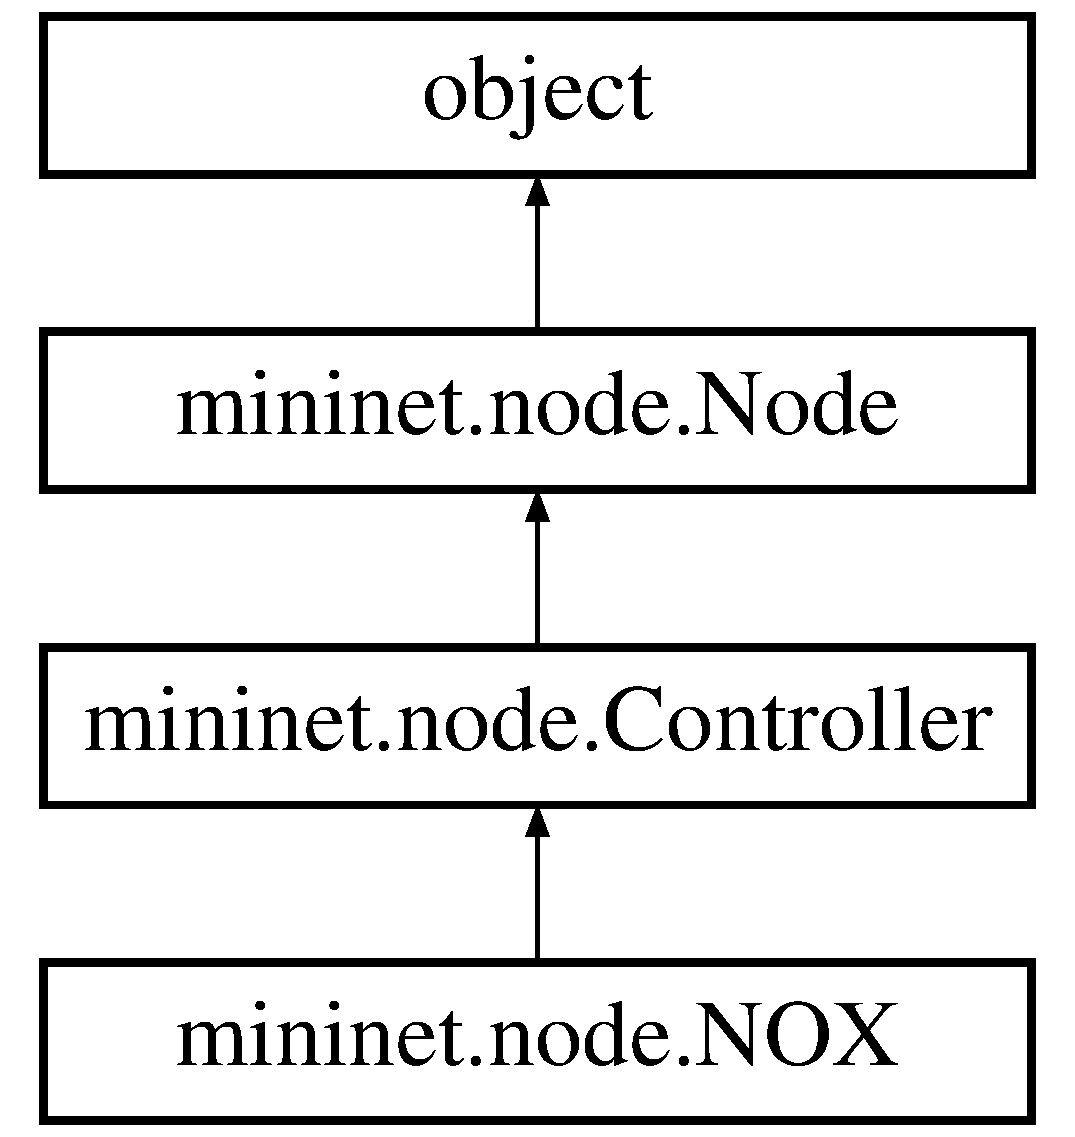
\includegraphics[height=4.000000cm]{classmininet_1_1node_1_1NOX}
\end{center}
\end{figure}
\subsection*{Public Member Functions}
\begin{DoxyCompactItemize}
\item 
def \hyperlink{classmininet_1_1node_1_1NOX_a48667ee571b5a8bf4ac9c022e3b68826}{\-\_\-\-\_\-init\-\_\-\-\_\-}
\end{DoxyCompactItemize}
\subsection*{Additional Inherited Members}


\subsection{Constructor \& Destructor Documentation}
\hypertarget{classmininet_1_1node_1_1NOX_a48667ee571b5a8bf4ac9c022e3b68826}{\index{mininet\-::node\-::\-N\-O\-X@{mininet\-::node\-::\-N\-O\-X}!\-\_\-\-\_\-init\-\_\-\-\_\-@{\-\_\-\-\_\-init\-\_\-\-\_\-}}
\index{\-\_\-\-\_\-init\-\_\-\-\_\-@{\-\_\-\-\_\-init\-\_\-\-\_\-}!mininet::node::NOX@{mininet\-::node\-::\-N\-O\-X}}
\subsubsection[{\-\_\-\-\_\-init\-\_\-\-\_\-}]{\setlength{\rightskip}{0pt plus 5cm}def mininet.\-node.\-N\-O\-X.\-\_\-\-\_\-init\-\_\-\-\_\- (
\begin{DoxyParamCaption}
\item[{}]{self, }
\item[{}]{name, }
\item[{}]{nox\-Args, }
\item[{}]{kwargs}
\end{DoxyParamCaption}
)}}\label{classmininet_1_1node_1_1NOX_a48667ee571b5a8bf4ac9c022e3b68826}
\begin{DoxyVerb}Init.
   name: name to give controller
   noxArgs: arguments (strings) to pass to NOX\end{DoxyVerb}
 

The documentation for this class was generated from the following file\-:\begin{DoxyCompactItemize}
\item 
node.\-py\end{DoxyCompactItemize}

\hypertarget{classmininet_1_1node_1_1OVSBridge}{\section{mininet.\-node.\-O\-V\-S\-Bridge Class Reference}
\label{classmininet_1_1node_1_1OVSBridge}\index{mininet.\-node.\-O\-V\-S\-Bridge@{mininet.\-node.\-O\-V\-S\-Bridge}}
}
Inheritance diagram for mininet.\-node.\-O\-V\-S\-Bridge\-:\begin{figure}[H]
\begin{center}
\leavevmode
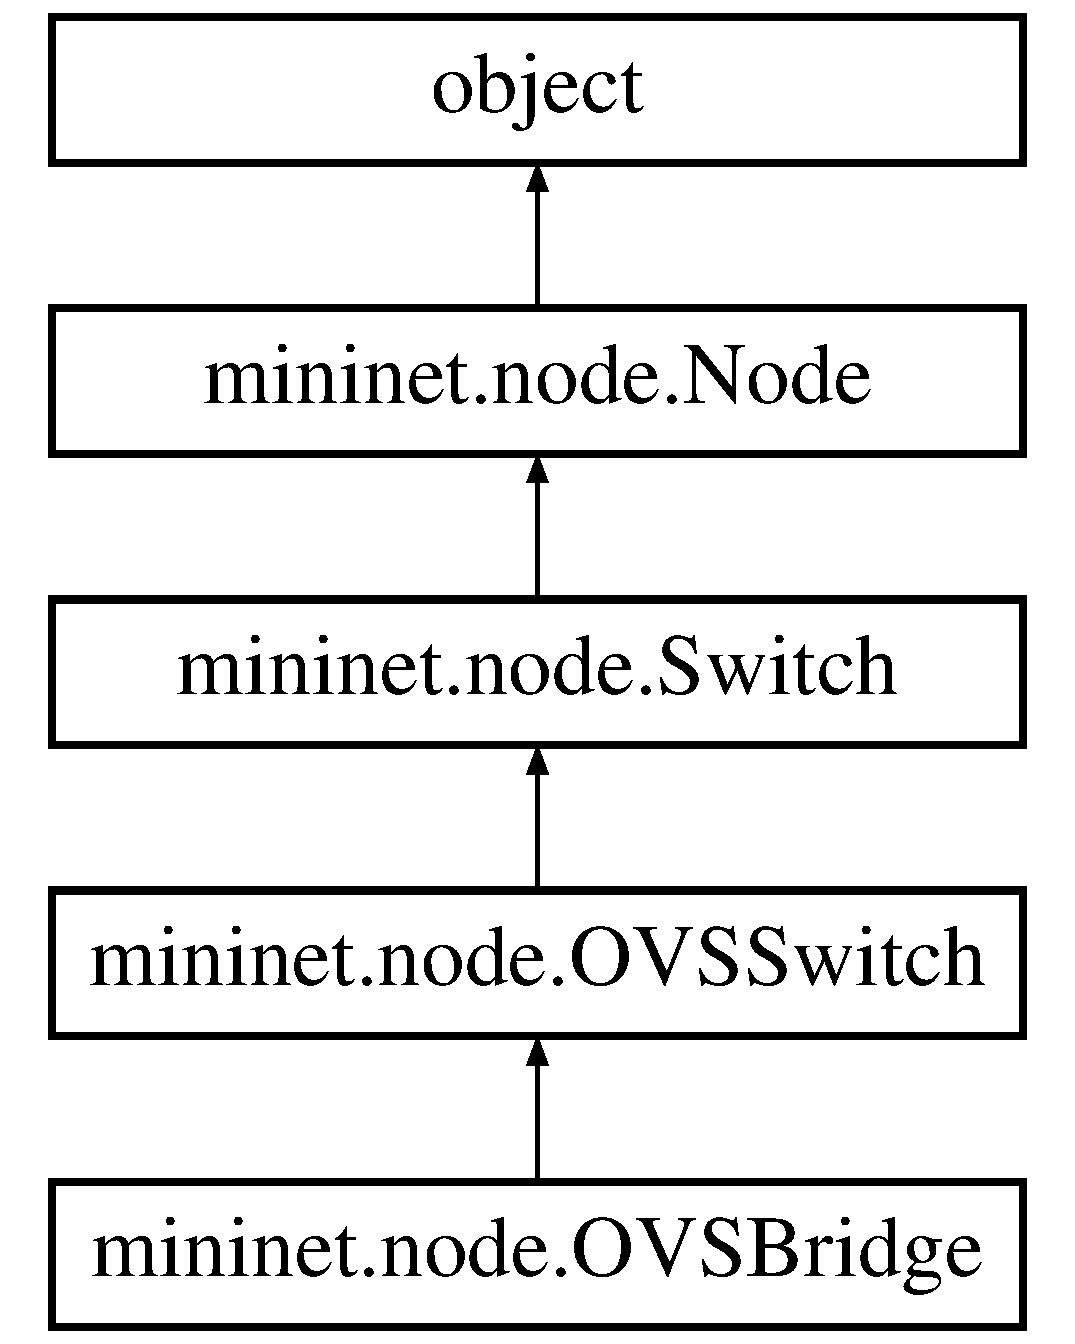
\includegraphics[height=5.000000cm]{classmininet_1_1node_1_1OVSBridge}
\end{center}
\end{figure}
\subsection*{Public Member Functions}
\begin{DoxyCompactItemize}
\item 
def \hyperlink{classmininet_1_1node_1_1OVSBridge_a5013ab60762b77fcdf899703c7256b14}{\-\_\-\-\_\-init\-\_\-\-\_\-}
\item 
\hypertarget{classmininet_1_1node_1_1OVSBridge_a0b9be8cb23cb358a09242807ff2fab37}{def {\bfseries start}}\label{classmininet_1_1node_1_1OVSBridge_a0b9be8cb23cb358a09242807ff2fab37}

\item 
\hypertarget{classmininet_1_1node_1_1OVSBridge_ab616ac07699ef0e09e861746a4d80265}{def {\bfseries connected}}\label{classmininet_1_1node_1_1OVSBridge_ab616ac07699ef0e09e861746a4d80265}

\end{DoxyCompactItemize}
\subsection*{Additional Inherited Members}


\subsection{Constructor \& Destructor Documentation}
\hypertarget{classmininet_1_1node_1_1OVSBridge_a5013ab60762b77fcdf899703c7256b14}{\index{mininet\-::node\-::\-O\-V\-S\-Bridge@{mininet\-::node\-::\-O\-V\-S\-Bridge}!\-\_\-\-\_\-init\-\_\-\-\_\-@{\-\_\-\-\_\-init\-\_\-\-\_\-}}
\index{\-\_\-\-\_\-init\-\_\-\-\_\-@{\-\_\-\-\_\-init\-\_\-\-\_\-}!mininet::node::OVSBridge@{mininet\-::node\-::\-O\-V\-S\-Bridge}}
\subsubsection[{\-\_\-\-\_\-init\-\_\-\-\_\-}]{\setlength{\rightskip}{0pt plus 5cm}def mininet.\-node.\-O\-V\-S\-Bridge.\-\_\-\-\_\-init\-\_\-\-\_\- (
\begin{DoxyParamCaption}
\item[{}]{self, }
\item[{}]{args, }
\item[{}]{kwargs}
\end{DoxyParamCaption}
)}}\label{classmininet_1_1node_1_1OVSBridge_a5013ab60762b77fcdf899703c7256b14}
\begin{DoxyVerb}stp: enable Spanning Tree Protocol (False)
   see OVSSwitch for other options\end{DoxyVerb}
 

The documentation for this class was generated from the following file\-:\begin{DoxyCompactItemize}
\item 
node.\-py\end{DoxyCompactItemize}

\hypertarget{classmininet_1_1node_1_1OVSController}{\section{mininet.\-node.\-O\-V\-S\-Controller Class Reference}
\label{classmininet_1_1node_1_1OVSController}\index{mininet.\-node.\-O\-V\-S\-Controller@{mininet.\-node.\-O\-V\-S\-Controller}}
}
Inheritance diagram for mininet.\-node.\-O\-V\-S\-Controller\-:\begin{figure}[H]
\begin{center}
\leavevmode
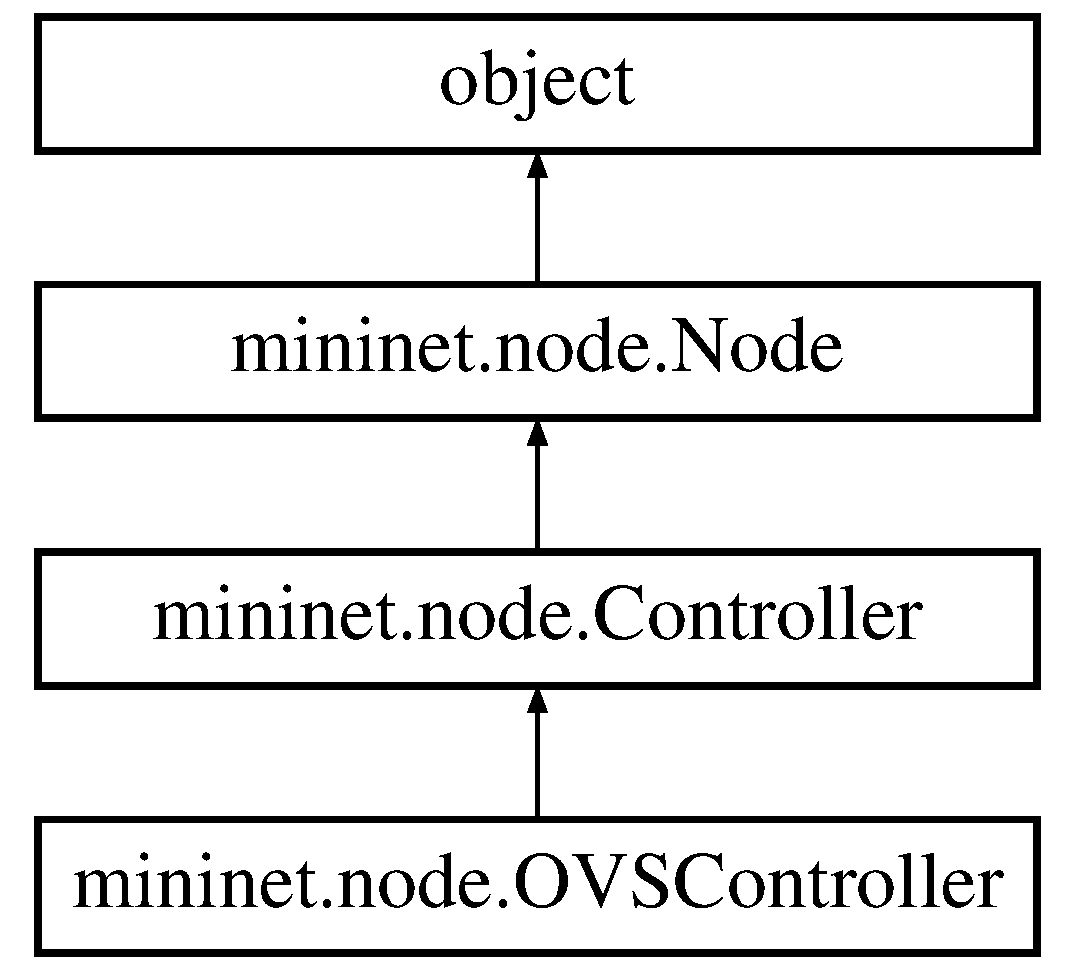
\includegraphics[height=4.000000cm]{classmininet_1_1node_1_1OVSController}
\end{center}
\end{figure}
\subsection*{Public Member Functions}
\begin{DoxyCompactItemize}
\item 
\hypertarget{classmininet_1_1node_1_1OVSController_a762db0702455de1de209205b977fe7e0}{def {\bfseries \-\_\-\-\_\-init\-\_\-\-\_\-}}\label{classmininet_1_1node_1_1OVSController_a762db0702455de1de209205b977fe7e0}

\item 
\hypertarget{classmininet_1_1node_1_1OVSController_a2ce3cc322466ab2cbcc27dc4aabaea65}{def {\bfseries is\-Available}}\label{classmininet_1_1node_1_1OVSController_a2ce3cc322466ab2cbcc27dc4aabaea65}

\end{DoxyCompactItemize}
\subsection*{Additional Inherited Members}


The documentation for this class was generated from the following file\-:\begin{DoxyCompactItemize}
\item 
node.\-py\end{DoxyCompactItemize}

\hypertarget{classmininet_1_1link_1_1OVSIntf}{\section{mininet.\-link.\-O\-V\-S\-Intf Class Reference}
\label{classmininet_1_1link_1_1OVSIntf}\index{mininet.\-link.\-O\-V\-S\-Intf@{mininet.\-link.\-O\-V\-S\-Intf}}
}
Inheritance diagram for mininet.\-link.\-O\-V\-S\-Intf\-:\begin{figure}[H]
\begin{center}
\leavevmode
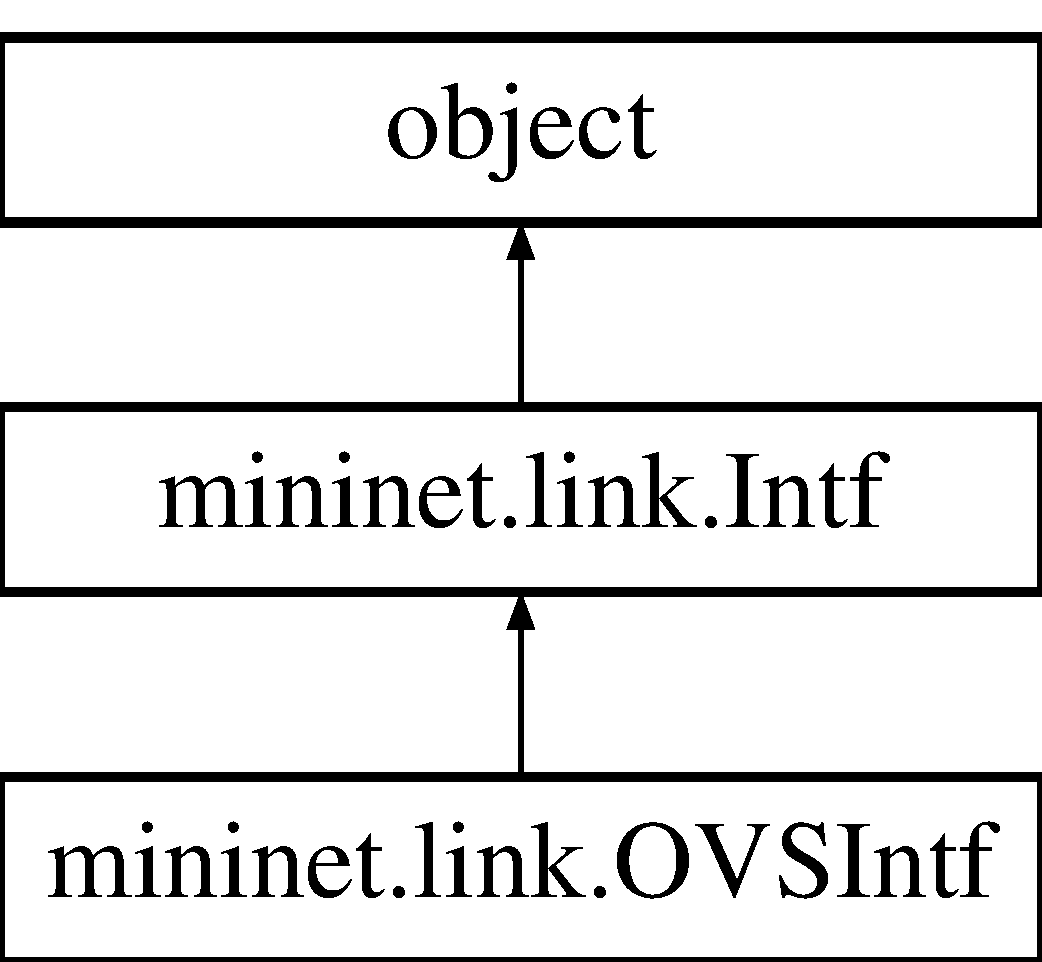
\includegraphics[height=3.000000cm]{classmininet_1_1link_1_1OVSIntf}
\end{center}
\end{figure}
\subsection*{Public Member Functions}
\begin{DoxyCompactItemize}
\item 
\hypertarget{classmininet_1_1link_1_1OVSIntf_aa133f507fede31a167fac6ac1e059563}{def {\bfseries ifconfig}}\label{classmininet_1_1link_1_1OVSIntf_aa133f507fede31a167fac6ac1e059563}

\end{DoxyCompactItemize}
\subsection*{Additional Inherited Members}


The documentation for this class was generated from the following file\-:\begin{DoxyCompactItemize}
\item 
link.\-py\end{DoxyCompactItemize}

\hypertarget{classmininet_1_1link_1_1OVSLink}{\section{mininet.\-link.\-O\-V\-S\-Link Class Reference}
\label{classmininet_1_1link_1_1OVSLink}\index{mininet.\-link.\-O\-V\-S\-Link@{mininet.\-link.\-O\-V\-S\-Link}}
}
Inheritance diagram for mininet.\-link.\-O\-V\-S\-Link\-:\begin{figure}[H]
\begin{center}
\leavevmode
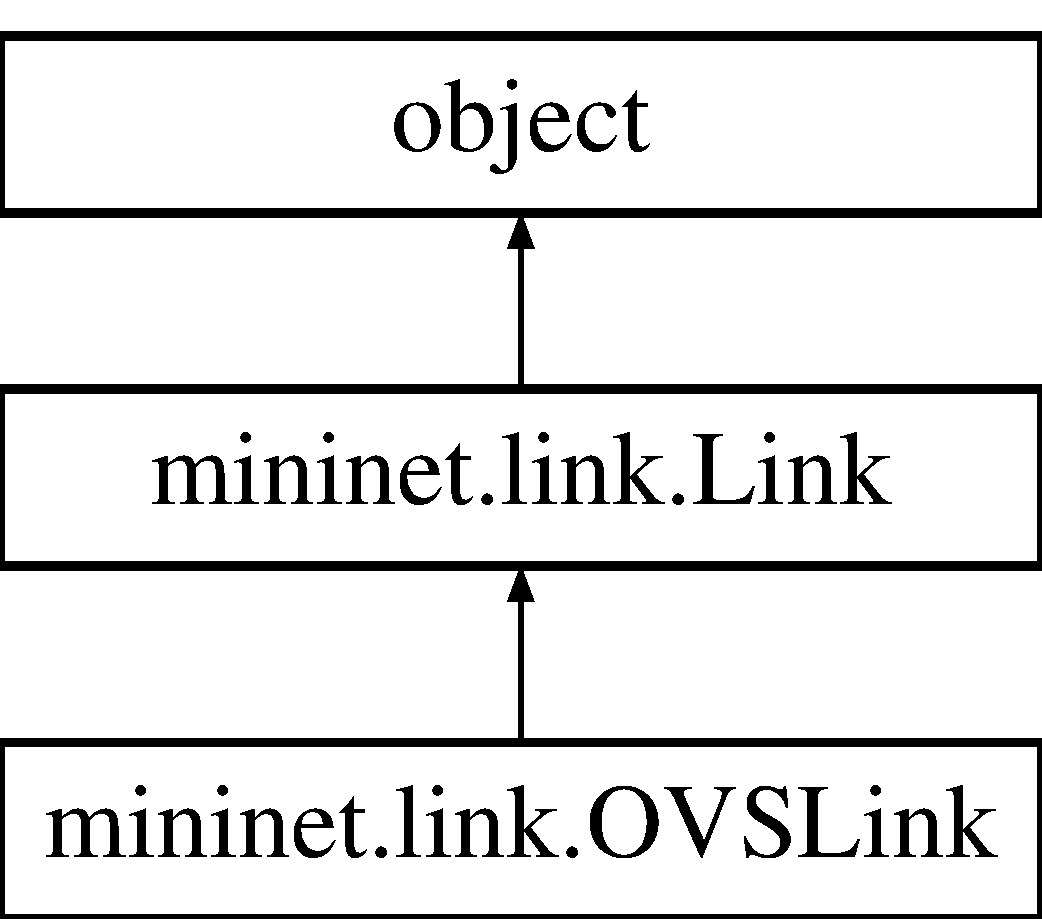
\includegraphics[height=3.000000cm]{classmininet_1_1link_1_1OVSLink}
\end{center}
\end{figure}
\subsection*{Public Member Functions}
\begin{DoxyCompactItemize}
\item 
\hypertarget{classmininet_1_1link_1_1OVSLink_a87c11ce7569403fe4829870adf8256d7}{def {\bfseries \-\_\-\-\_\-init\-\_\-\-\_\-}}\label{classmininet_1_1link_1_1OVSLink_a87c11ce7569403fe4829870adf8256d7}

\item 
\hypertarget{classmininet_1_1link_1_1OVSLink_ad9cd6272bde17df17140a0b37b884e50}{def {\bfseries make\-Intf\-Pair}}\label{classmininet_1_1link_1_1OVSLink_ad9cd6272bde17df17140a0b37b884e50}

\end{DoxyCompactItemize}
\subsection*{Public Attributes}
\begin{DoxyCompactItemize}
\item 
\hypertarget{classmininet_1_1link_1_1OVSLink_a25082afab9dd72f193cd35fff083c7bd}{{\bfseries is\-Patch\-Link}}\label{classmininet_1_1link_1_1OVSLink_a25082afab9dd72f193cd35fff083c7bd}

\end{DoxyCompactItemize}


\subsection{Detailed Description}
\begin{DoxyVerb}Link that makes patch links between OVSSwitches
   Warning: in testing we have found that no more
   than ~64 OVS patch links should be used in row.\end{DoxyVerb}
 

The documentation for this class was generated from the following file\-:\begin{DoxyCompactItemize}
\item 
link.\-py\end{DoxyCompactItemize}

\hypertarget{classmininet_1_1node_1_1OVSSwitch}{\section{mininet.\-node.\-O\-V\-S\-Switch Class Reference}
\label{classmininet_1_1node_1_1OVSSwitch}\index{mininet.\-node.\-O\-V\-S\-Switch@{mininet.\-node.\-O\-V\-S\-Switch}}
}
Inheritance diagram for mininet.\-node.\-O\-V\-S\-Switch\-:\begin{figure}[H]
\begin{center}
\leavevmode
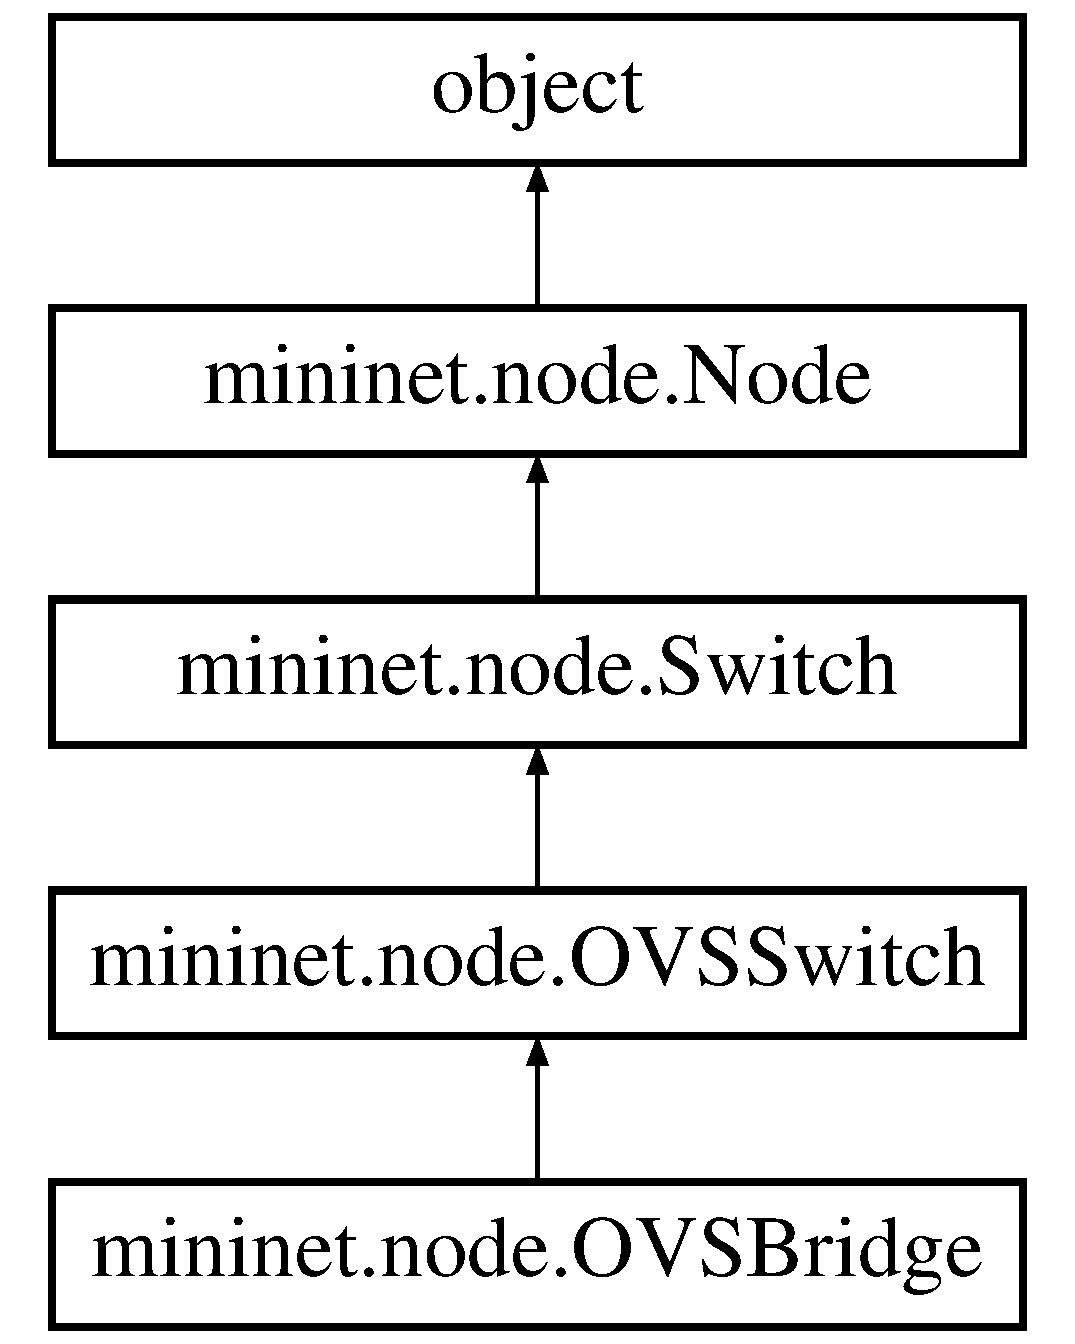
\includegraphics[height=5.000000cm]{classmininet_1_1node_1_1OVSSwitch}
\end{center}
\end{figure}
\subsection*{Public Member Functions}
\begin{DoxyCompactItemize}
\item 
def \hyperlink{classmininet_1_1node_1_1OVSSwitch_ab5db2ef0d48302217833ce1538270310}{\-\_\-\-\_\-init\-\_\-\-\_\-}
\item 
\hypertarget{classmininet_1_1node_1_1OVSSwitch_a429a17cd26b37e4f7a58a1c9162120dc}{def {\bfseries setup}}\label{classmininet_1_1node_1_1OVSSwitch_a429a17cd26b37e4f7a58a1c9162120dc}

\item 
\hypertarget{classmininet_1_1node_1_1OVSSwitch_a81eeea1dc5162325ddbb2c07039b53de}{def {\bfseries is\-Old\-O\-V\-S}}\label{classmininet_1_1node_1_1OVSSwitch_a81eeea1dc5162325ddbb2c07039b53de}

\item 
\hypertarget{classmininet_1_1node_1_1OVSSwitch_a70306fa47e76fb9f4d3317dc88bf72ba}{def {\bfseries dpctl}}\label{classmininet_1_1node_1_1OVSSwitch_a70306fa47e76fb9f4d3317dc88bf72ba}

\item 
\hypertarget{classmininet_1_1node_1_1OVSSwitch_ae5eadfb6af415639ca3731e35563f661}{def {\bfseries vsctl}}\label{classmininet_1_1node_1_1OVSSwitch_ae5eadfb6af415639ca3731e35563f661}

\item 
\hypertarget{classmininet_1_1node_1_1OVSSwitch_aa3e0723a5b433fe03bbb4c39ab09c2c8}{def {\bfseries attach}}\label{classmininet_1_1node_1_1OVSSwitch_aa3e0723a5b433fe03bbb4c39ab09c2c8}

\item 
\hypertarget{classmininet_1_1node_1_1OVSSwitch_ab1cf861fc1db0a14244f650d0bb1aa93}{def {\bfseries detach}}\label{classmininet_1_1node_1_1OVSSwitch_ab1cf861fc1db0a14244f650d0bb1aa93}

\item 
def \hyperlink{classmininet_1_1node_1_1OVSSwitch_a14878a75c1db9c5aa4579471d0ece748}{controller\-U\-U\-I\-Ds}
\item 
\hypertarget{classmininet_1_1node_1_1OVSSwitch_abdc44068e907814e5aae52fef9ea4e3a}{def {\bfseries connected}}\label{classmininet_1_1node_1_1OVSSwitch_abdc44068e907814e5aae52fef9ea4e3a}

\item 
\hypertarget{classmininet_1_1node_1_1OVSSwitch_aaabdfd2c0413735604bba55bcef66dff}{def {\bfseries intf\-Opts}}\label{classmininet_1_1node_1_1OVSSwitch_aaabdfd2c0413735604bba55bcef66dff}

\item 
\hypertarget{classmininet_1_1node_1_1OVSSwitch_af82b359e514f8e4604958152c3b81f60}{def {\bfseries bridge\-Opts}}\label{classmininet_1_1node_1_1OVSSwitch_af82b359e514f8e4604958152c3b81f60}

\item 
\hypertarget{classmininet_1_1node_1_1OVSSwitch_a64175be004c3bca8217799640b168d41}{def {\bfseries start}}\label{classmininet_1_1node_1_1OVSSwitch_a64175be004c3bca8217799640b168d41}

\item 
def \hyperlink{classmininet_1_1node_1_1OVSSwitch_ac68c5ffcb307298b105cf664b8b170e6}{batch\-Startup}
\item 
def \hyperlink{classmininet_1_1node_1_1OVSSwitch_a738aa9dc6c54527fee71f09aea9da8aa}{stop}
\item 
\hypertarget{classmininet_1_1node_1_1OVSSwitch_a2ab791e35f567b35a92c03dd9c89389d}{def {\bfseries batch\-Shutdown}}\label{classmininet_1_1node_1_1OVSSwitch_a2ab791e35f567b35a92c03dd9c89389d}

\end{DoxyCompactItemize}
\subsection*{Static Public Member Functions}
\begin{DoxyCompactItemize}
\item 
def \hyperlink{classmininet_1_1node_1_1OVSSwitch_a91f455741115c89f17d428cd8c22f284}{T\-C\-Reapply}
\end{DoxyCompactItemize}
\subsection*{Public Attributes}
\begin{DoxyCompactItemize}
\item 
\hypertarget{classmininet_1_1node_1_1OVSSwitch_a2a20caf43bb3fc4aab23025386d2c030}{{\bfseries fail\-Mode}}\label{classmininet_1_1node_1_1OVSSwitch_a2a20caf43bb3fc4aab23025386d2c030}

\item 
\hypertarget{classmininet_1_1node_1_1OVSSwitch_a7debf01783ed919fa2234f13c1982a43}{{\bfseries datapath}}\label{classmininet_1_1node_1_1OVSSwitch_a7debf01783ed919fa2234f13c1982a43}

\item 
\hypertarget{classmininet_1_1node_1_1OVSSwitch_a7e14ba5b1de8746f715b362c56200e4e}{{\bfseries inband}}\label{classmininet_1_1node_1_1OVSSwitch_a7e14ba5b1de8746f715b362c56200e4e}

\item 
\hypertarget{classmininet_1_1node_1_1OVSSwitch_a165ea494ac02c26dc67be5e357f41da3}{{\bfseries protocols}}\label{classmininet_1_1node_1_1OVSSwitch_a165ea494ac02c26dc67be5e357f41da3}

\item 
\hypertarget{classmininet_1_1node_1_1OVSSwitch_a675011761bb9860ef2681098139f930c}{{\bfseries reconnectms}}\label{classmininet_1_1node_1_1OVSSwitch_a675011761bb9860ef2681098139f930c}

\item 
\hypertarget{classmininet_1_1node_1_1OVSSwitch_aea9d7656773272b66ae551645be6e1b1}{{\bfseries stp}}\label{classmininet_1_1node_1_1OVSSwitch_aea9d7656773272b66ae551645be6e1b1}

\item 
\hypertarget{classmininet_1_1node_1_1OVSSwitch_a0f66cf402129bf13d83082c7139333f2}{{\bfseries batch}}\label{classmininet_1_1node_1_1OVSSwitch_a0f66cf402129bf13d83082c7139333f2}

\item 
\hypertarget{classmininet_1_1node_1_1OVSSwitch_aaa9afa54900f91c2140b961f34421004}{{\bfseries commands}}\label{classmininet_1_1node_1_1OVSSwitch_aaa9afa54900f91c2140b961f34421004}

\end{DoxyCompactItemize}
\subsection*{Static Public Attributes}
\begin{DoxyCompactItemize}
\item 
\hypertarget{classmininet_1_1node_1_1OVSSwitch_a7dfeb938c6038b8b47001ef6e9a78e44}{int {\bfseries argmax} = 128000}\label{classmininet_1_1node_1_1OVSSwitch_a7dfeb938c6038b8b47001ef6e9a78e44}

\end{DoxyCompactItemize}


\subsection{Constructor \& Destructor Documentation}
\hypertarget{classmininet_1_1node_1_1OVSSwitch_ab5db2ef0d48302217833ce1538270310}{\index{mininet\-::node\-::\-O\-V\-S\-Switch@{mininet\-::node\-::\-O\-V\-S\-Switch}!\-\_\-\-\_\-init\-\_\-\-\_\-@{\-\_\-\-\_\-init\-\_\-\-\_\-}}
\index{\-\_\-\-\_\-init\-\_\-\-\_\-@{\-\_\-\-\_\-init\-\_\-\-\_\-}!mininet::node::OVSSwitch@{mininet\-::node\-::\-O\-V\-S\-Switch}}
\subsubsection[{\-\_\-\-\_\-init\-\_\-\-\_\-}]{\setlength{\rightskip}{0pt plus 5cm}def mininet.\-node.\-O\-V\-S\-Switch.\-\_\-\-\_\-init\-\_\-\-\_\- (
\begin{DoxyParamCaption}
\item[{}]{self, }
\item[{}]{name, }
\item[{}]{fail\-Mode = {\ttfamily 'secure'}, }
\item[{}]{datapath = {\ttfamily 'kernel'}, }
\item[{}]{inband = {\ttfamily False}, }
\item[{}]{protocols = {\ttfamily None}, }
\item[{}]{reconnectms = {\ttfamily 1000}, }
\item[{}]{stp = {\ttfamily False}, }
\item[{}]{batch = {\ttfamily False}, }
\item[{}]{params}
\end{DoxyParamCaption}
)}}\label{classmininet_1_1node_1_1OVSSwitch_ab5db2ef0d48302217833ce1538270310}
\begin{DoxyVerb}name: name for switch
   failMode: controller loss behavior (secure|open)
   datapath: userspace or kernel mode (kernel|user)
   inband: use in-band control (False)
   protocols: use specific OpenFlow version(s) (e.g. OpenFlow13)
      Unspecified (or old OVS version) uses OVS default
   reconnectms: max reconnect timeout in ms (0/None for default)
   stp: enable STP (False, requires failMode=standalone)
   batch: enable batch startup (False)\end{DoxyVerb}
 

\subsection{Member Function Documentation}
\hypertarget{classmininet_1_1node_1_1OVSSwitch_ac68c5ffcb307298b105cf664b8b170e6}{\index{mininet\-::node\-::\-O\-V\-S\-Switch@{mininet\-::node\-::\-O\-V\-S\-Switch}!batch\-Startup@{batch\-Startup}}
\index{batch\-Startup@{batch\-Startup}!mininet::node::OVSSwitch@{mininet\-::node\-::\-O\-V\-S\-Switch}}
\subsubsection[{batch\-Startup}]{\setlength{\rightskip}{0pt plus 5cm}def mininet.\-node.\-O\-V\-S\-Switch.\-batch\-Startup (
\begin{DoxyParamCaption}
\item[{}]{cls, }
\item[{}]{switches, }
\item[{}]{run = {\ttfamily errRun}}
\end{DoxyParamCaption}
)}}\label{classmininet_1_1node_1_1OVSSwitch_ac68c5ffcb307298b105cf664b8b170e6}
\begin{DoxyVerb}Batch startup for OVS
   switches: switches to start up
   run: function to run commands (errRun)\end{DoxyVerb}
 \hypertarget{classmininet_1_1node_1_1OVSSwitch_a14878a75c1db9c5aa4579471d0ece748}{\index{mininet\-::node\-::\-O\-V\-S\-Switch@{mininet\-::node\-::\-O\-V\-S\-Switch}!controller\-U\-U\-I\-Ds@{controller\-U\-U\-I\-Ds}}
\index{controller\-U\-U\-I\-Ds@{controller\-U\-U\-I\-Ds}!mininet::node::OVSSwitch@{mininet\-::node\-::\-O\-V\-S\-Switch}}
\subsubsection[{controller\-U\-U\-I\-Ds}]{\setlength{\rightskip}{0pt plus 5cm}def mininet.\-node.\-O\-V\-S\-Switch.\-controller\-U\-U\-I\-Ds (
\begin{DoxyParamCaption}
\item[{}]{self, }
\item[{}]{update = {\ttfamily False}}
\end{DoxyParamCaption}
)}}\label{classmininet_1_1node_1_1OVSSwitch_a14878a75c1db9c5aa4579471d0ece748}
\begin{DoxyVerb}Return ovsdb UUIDs for our controllers
   update: update cached value\end{DoxyVerb}
 \hypertarget{classmininet_1_1node_1_1OVSSwitch_a738aa9dc6c54527fee71f09aea9da8aa}{\index{mininet\-::node\-::\-O\-V\-S\-Switch@{mininet\-::node\-::\-O\-V\-S\-Switch}!stop@{stop}}
\index{stop@{stop}!mininet::node::OVSSwitch@{mininet\-::node\-::\-O\-V\-S\-Switch}}
\subsubsection[{stop}]{\setlength{\rightskip}{0pt plus 5cm}def mininet.\-node.\-O\-V\-S\-Switch.\-stop (
\begin{DoxyParamCaption}
\item[{}]{self, }
\item[{}]{delete\-Intfs = {\ttfamily True}}
\end{DoxyParamCaption}
)}}\label{classmininet_1_1node_1_1OVSSwitch_a738aa9dc6c54527fee71f09aea9da8aa}
\begin{DoxyVerb}Terminate OVS switch.
   deleteIntfs: delete interfaces? (True)\end{DoxyVerb}
 \hypertarget{classmininet_1_1node_1_1OVSSwitch_a91f455741115c89f17d428cd8c22f284}{\index{mininet\-::node\-::\-O\-V\-S\-Switch@{mininet\-::node\-::\-O\-V\-S\-Switch}!T\-C\-Reapply@{T\-C\-Reapply}}
\index{T\-C\-Reapply@{T\-C\-Reapply}!mininet::node::OVSSwitch@{mininet\-::node\-::\-O\-V\-S\-Switch}}
\subsubsection[{T\-C\-Reapply}]{\setlength{\rightskip}{0pt plus 5cm}def mininet.\-node.\-O\-V\-S\-Switch.\-T\-C\-Reapply (
\begin{DoxyParamCaption}
\item[{}]{intf}
\end{DoxyParamCaption}
)\hspace{0.3cm}{\ttfamily [static]}}}\label{classmininet_1_1node_1_1OVSSwitch_a91f455741115c89f17d428cd8c22f284}
\begin{DoxyVerb}Unfortunately OVS and Mininet are fighting
   over tc queuing disciplines. As a quick hack/
   workaround, we clear OVS's and reapply our own.\end{DoxyVerb}
 

The documentation for this class was generated from the following file\-:\begin{DoxyCompactItemize}
\item 
node.\-py\end{DoxyCompactItemize}

\hypertarget{classmininet_1_1wifiPlot_1_1plot}{\section{mininet.\-wifi\-Plot.\-plot Class Reference}
\label{classmininet_1_1wifiPlot_1_1plot}\index{mininet.\-wifi\-Plot.\-plot@{mininet.\-wifi\-Plot.\-plot}}
}
Inheritance diagram for mininet.\-wifi\-Plot.\-plot\-:\begin{figure}[H]
\begin{center}
\leavevmode
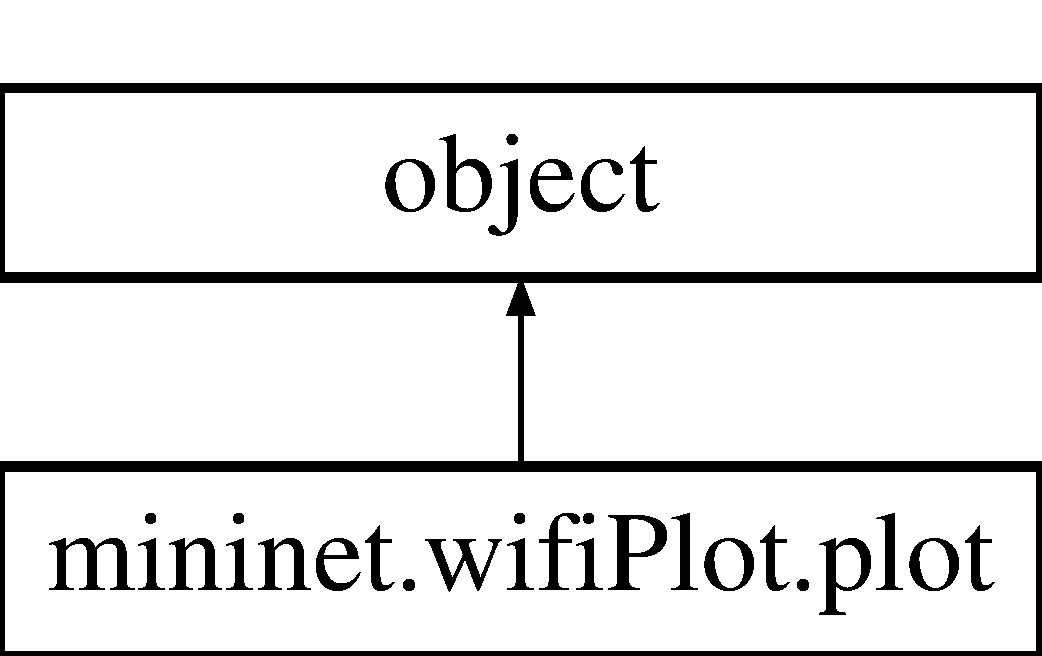
\includegraphics[height=2.000000cm]{classmininet_1_1wifiPlot_1_1plot}
\end{center}
\end{figure}
\subsection*{Public Member Functions}
\begin{DoxyCompactItemize}
\item 
def \hyperlink{classmininet_1_1wifiPlot_1_1plot_a16e07a7c655bcf1704011a677e82e3b7}{close\-Plot}
\item 
def \hyperlink{classmininet_1_1wifiPlot_1_1plot_a95c9ae54e6cef33f10203d098358fac4}{draw\-Node}
\item 
def \hyperlink{classmininet_1_1wifiPlot_1_1plot_abdfdf0d24468b5cf95c48c654dc033c9}{draw\-Txt}
\item 
def \hyperlink{classmininet_1_1wifiPlot_1_1plot_ab15b99dd9089f2da38aa7d245d9ec93f}{draw\-Circle}
\item 
def \hyperlink{classmininet_1_1wifiPlot_1_1plot_ab5ec203809c86f599838a22ee7603d69}{graph\-Update}
\item 
def \hyperlink{classmininet_1_1wifiPlot_1_1plot_af288f91f175e6a7694153fe2ba610dab}{plot\-Draw}
\item 
def \hyperlink{classmininet_1_1wifiPlot_1_1plot_a02d84da948e4442329345e5ae4f3be25}{plot\-Scatter}
\item 
def \hyperlink{classmininet_1_1wifiPlot_1_1plot_ac481c27201492c944bd9626e6e794b60}{plot\-Line2d}
\item 
def \hyperlink{classmininet_1_1wifiPlot_1_1plot_a731bdfc39255d8a3fcd83728ae51d37d}{plot\-Line\-Txt}
\item 
def \hyperlink{classmininet_1_1wifiPlot_1_1plot_a52436c39966631f6038855adaeffff88}{plot\-Line}
\item 
def \hyperlink{classmininet_1_1wifiPlot_1_1plot_abf2babf19c2a94ddc21f4ade3a6edce8}{instantiate\-Graph}
\item 
def \hyperlink{classmininet_1_1wifiPlot_1_1plot_a91bcdaa91049db2ebf8ee02b92330021}{instantiate\-Node}
\item 
\hypertarget{classmininet_1_1wifiPlot_1_1plot_adad8a800d48b1720a3022598cf447760}{def {\bfseries update\-Circle\-Radius}}\label{classmininet_1_1wifiPlot_1_1plot_adad8a800d48b1720a3022598cf447760}

\item 
def \hyperlink{classmininet_1_1wifiPlot_1_1plot_ac962d93dca5cf6ef7fc71e38e2b22b2f}{instantiate\-Circle}
\item 
def \hyperlink{classmininet_1_1wifiPlot_1_1plot_a428302bd589ef359c6f3463495bf243e}{instantiate\-Annotate}
\end{DoxyCompactItemize}
\subsection*{Static Public Attributes}
\begin{DoxyCompactItemize}
\item 
\hypertarget{classmininet_1_1wifiPlot_1_1plot_a55efe84a502db8a56969c35a58d6f212}{list {\bfseries nodes\-Plotted} = \mbox{[}$\,$\mbox{]}}\label{classmininet_1_1wifiPlot_1_1plot_a55efe84a502db8a56969c35a58d6f212}

\item 
\hypertarget{classmininet_1_1wifiPlot_1_1plot_aba5c7af14e7f8b749e4dae705078404c}{dictionary {\bfseries plt\-Circle} = \{\}}\label{classmininet_1_1wifiPlot_1_1plot_aba5c7af14e7f8b749e4dae705078404c}

\item 
\hypertarget{classmininet_1_1wifiPlot_1_1plot_a1c6d625353e15d07983b866c99386cd2}{dictionary {\bfseries plt\-Node} = \{\}}\label{classmininet_1_1wifiPlot_1_1plot_a1c6d625353e15d07983b866c99386cd2}

\item 
\hypertarget{classmininet_1_1wifiPlot_1_1plot_a64ba0df28f6fe244612bba36ac5b6cc0}{dictionary {\bfseries plttxt} = \{\}}\label{classmininet_1_1wifiPlot_1_1plot_a64ba0df28f6fe244612bba36ac5b6cc0}

\item 
\hypertarget{classmininet_1_1wifiPlot_1_1plot_a0ee7829b93a5f88edfc4d57a639fdaec}{{\bfseries ax} = None}\label{classmininet_1_1wifiPlot_1_1plot_a0ee7829b93a5f88edfc4d57a639fdaec}

\end{DoxyCompactItemize}


\subsection{Member Function Documentation}
\hypertarget{classmininet_1_1wifiPlot_1_1plot_a16e07a7c655bcf1704011a677e82e3b7}{\index{mininet\-::wifi\-Plot\-::plot@{mininet\-::wifi\-Plot\-::plot}!close\-Plot@{close\-Plot}}
\index{close\-Plot@{close\-Plot}!mininet::wifiPlot::plot@{mininet\-::wifi\-Plot\-::plot}}
\subsubsection[{close\-Plot}]{\setlength{\rightskip}{0pt plus 5cm}def mininet.\-wifi\-Plot.\-plot.\-close\-Plot (
\begin{DoxyParamCaption}
\item[{}]{self}
\end{DoxyParamCaption}
)}}\label{classmininet_1_1wifiPlot_1_1plot_a16e07a7c655bcf1704011a677e82e3b7}
\begin{DoxyVerb}Close\end{DoxyVerb}
 \hypertarget{classmininet_1_1wifiPlot_1_1plot_ab15b99dd9089f2da38aa7d245d9ec93f}{\index{mininet\-::wifi\-Plot\-::plot@{mininet\-::wifi\-Plot\-::plot}!draw\-Circle@{draw\-Circle}}
\index{draw\-Circle@{draw\-Circle}!mininet::wifiPlot::plot@{mininet\-::wifi\-Plot\-::plot}}
\subsubsection[{draw\-Circle}]{\setlength{\rightskip}{0pt plus 5cm}def mininet.\-wifi\-Plot.\-plot.\-draw\-Circle (
\begin{DoxyParamCaption}
\item[{}]{self, }
\item[{}]{node}
\end{DoxyParamCaption}
)}}\label{classmininet_1_1wifiPlot_1_1plot_ab15b99dd9089f2da38aa7d245d9ec93f}
\begin{DoxyVerb}drawCircle\end{DoxyVerb}
 \hypertarget{classmininet_1_1wifiPlot_1_1plot_a95c9ae54e6cef33f10203d098358fac4}{\index{mininet\-::wifi\-Plot\-::plot@{mininet\-::wifi\-Plot\-::plot}!draw\-Node@{draw\-Node}}
\index{draw\-Node@{draw\-Node}!mininet::wifiPlot::plot@{mininet\-::wifi\-Plot\-::plot}}
\subsubsection[{draw\-Node}]{\setlength{\rightskip}{0pt plus 5cm}def mininet.\-wifi\-Plot.\-plot.\-draw\-Node (
\begin{DoxyParamCaption}
\item[{}]{self, }
\item[{}]{node}
\end{DoxyParamCaption}
)}}\label{classmininet_1_1wifiPlot_1_1plot_a95c9ae54e6cef33f10203d098358fac4}
\begin{DoxyVerb}Update Draw\end{DoxyVerb}
 \hypertarget{classmininet_1_1wifiPlot_1_1plot_abdfdf0d24468b5cf95c48c654dc033c9}{\index{mininet\-::wifi\-Plot\-::plot@{mininet\-::wifi\-Plot\-::plot}!draw\-Txt@{draw\-Txt}}
\index{draw\-Txt@{draw\-Txt}!mininet::wifiPlot::plot@{mininet\-::wifi\-Plot\-::plot}}
\subsubsection[{draw\-Txt}]{\setlength{\rightskip}{0pt plus 5cm}def mininet.\-wifi\-Plot.\-plot.\-draw\-Txt (
\begin{DoxyParamCaption}
\item[{}]{self, }
\item[{}]{node}
\end{DoxyParamCaption}
)}}\label{classmininet_1_1wifiPlot_1_1plot_abdfdf0d24468b5cf95c48c654dc033c9}
\begin{DoxyVerb}drawTxt\end{DoxyVerb}
 \hypertarget{classmininet_1_1wifiPlot_1_1plot_ab5ec203809c86f599838a22ee7603d69}{\index{mininet\-::wifi\-Plot\-::plot@{mininet\-::wifi\-Plot\-::plot}!graph\-Update@{graph\-Update}}
\index{graph\-Update@{graph\-Update}!mininet::wifiPlot::plot@{mininet\-::wifi\-Plot\-::plot}}
\subsubsection[{graph\-Update}]{\setlength{\rightskip}{0pt plus 5cm}def mininet.\-wifi\-Plot.\-plot.\-graph\-Update (
\begin{DoxyParamCaption}
\item[{}]{self, }
\item[{}]{node}
\end{DoxyParamCaption}
)}}\label{classmininet_1_1wifiPlot_1_1plot_ab5ec203809c86f599838a22ee7603d69}
\begin{DoxyVerb}Update Graph\end{DoxyVerb}
 \hypertarget{classmininet_1_1wifiPlot_1_1plot_a428302bd589ef359c6f3463495bf243e}{\index{mininet\-::wifi\-Plot\-::plot@{mininet\-::wifi\-Plot\-::plot}!instantiate\-Annotate@{instantiate\-Annotate}}
\index{instantiate\-Annotate@{instantiate\-Annotate}!mininet::wifiPlot::plot@{mininet\-::wifi\-Plot\-::plot}}
\subsubsection[{instantiate\-Annotate}]{\setlength{\rightskip}{0pt plus 5cm}def mininet.\-wifi\-Plot.\-plot.\-instantiate\-Annotate (
\begin{DoxyParamCaption}
\item[{}]{self, }
\item[{}]{node}
\end{DoxyParamCaption}
)}}\label{classmininet_1_1wifiPlot_1_1plot_a428302bd589ef359c6f3463495bf243e}
\begin{DoxyVerb}instantiateAnnotate\end{DoxyVerb}
 \hypertarget{classmininet_1_1wifiPlot_1_1plot_ac962d93dca5cf6ef7fc71e38e2b22b2f}{\index{mininet\-::wifi\-Plot\-::plot@{mininet\-::wifi\-Plot\-::plot}!instantiate\-Circle@{instantiate\-Circle}}
\index{instantiate\-Circle@{instantiate\-Circle}!mininet::wifiPlot::plot@{mininet\-::wifi\-Plot\-::plot}}
\subsubsection[{instantiate\-Circle}]{\setlength{\rightskip}{0pt plus 5cm}def mininet.\-wifi\-Plot.\-plot.\-instantiate\-Circle (
\begin{DoxyParamCaption}
\item[{}]{self, }
\item[{}]{node}
\end{DoxyParamCaption}
)}}\label{classmininet_1_1wifiPlot_1_1plot_ac962d93dca5cf6ef7fc71e38e2b22b2f}
\begin{DoxyVerb}instantiateCircle\end{DoxyVerb}
 \hypertarget{classmininet_1_1wifiPlot_1_1plot_abf2babf19c2a94ddc21f4ade3a6edce8}{\index{mininet\-::wifi\-Plot\-::plot@{mininet\-::wifi\-Plot\-::plot}!instantiate\-Graph@{instantiate\-Graph}}
\index{instantiate\-Graph@{instantiate\-Graph}!mininet::wifiPlot::plot@{mininet\-::wifi\-Plot\-::plot}}
\subsubsection[{instantiate\-Graph}]{\setlength{\rightskip}{0pt plus 5cm}def mininet.\-wifi\-Plot.\-plot.\-instantiate\-Graph (
\begin{DoxyParamCaption}
\item[{}]{self, }
\item[{}]{M\-A\-X\-\_\-\-X, }
\item[{}]{M\-A\-X\-\_\-\-Y}
\end{DoxyParamCaption}
)}}\label{classmininet_1_1wifiPlot_1_1plot_abf2babf19c2a94ddc21f4ade3a6edce8}
\begin{DoxyVerb}instantiateGraph\end{DoxyVerb}
 \hypertarget{classmininet_1_1wifiPlot_1_1plot_a91bcdaa91049db2ebf8ee02b92330021}{\index{mininet\-::wifi\-Plot\-::plot@{mininet\-::wifi\-Plot\-::plot}!instantiate\-Node@{instantiate\-Node}}
\index{instantiate\-Node@{instantiate\-Node}!mininet::wifiPlot::plot@{mininet\-::wifi\-Plot\-::plot}}
\subsubsection[{instantiate\-Node}]{\setlength{\rightskip}{0pt plus 5cm}def mininet.\-wifi\-Plot.\-plot.\-instantiate\-Node (
\begin{DoxyParamCaption}
\item[{}]{self, }
\item[{}]{node, }
\item[{}]{M\-A\-X\-\_\-\-X, }
\item[{}]{M\-A\-X\-\_\-\-Y}
\end{DoxyParamCaption}
)}}\label{classmininet_1_1wifiPlot_1_1plot_a91bcdaa91049db2ebf8ee02b92330021}
\begin{DoxyVerb}instantiateNode\end{DoxyVerb}
 \hypertarget{classmininet_1_1wifiPlot_1_1plot_af288f91f175e6a7694153fe2ba610dab}{\index{mininet\-::wifi\-Plot\-::plot@{mininet\-::wifi\-Plot\-::plot}!plot\-Draw@{plot\-Draw}}
\index{plot\-Draw@{plot\-Draw}!mininet::wifiPlot::plot@{mininet\-::wifi\-Plot\-::plot}}
\subsubsection[{plot\-Draw}]{\setlength{\rightskip}{0pt plus 5cm}def mininet.\-wifi\-Plot.\-plot.\-plot\-Draw (
\begin{DoxyParamCaption}
\item[{}]{self}
\end{DoxyParamCaption}
)}}\label{classmininet_1_1wifiPlot_1_1plot_af288f91f175e6a7694153fe2ba610dab}
\begin{DoxyVerb}plotDraw\end{DoxyVerb}
 \hypertarget{classmininet_1_1wifiPlot_1_1plot_a52436c39966631f6038855adaeffff88}{\index{mininet\-::wifi\-Plot\-::plot@{mininet\-::wifi\-Plot\-::plot}!plot\-Line@{plot\-Line}}
\index{plot\-Line@{plot\-Line}!mininet::wifiPlot::plot@{mininet\-::wifi\-Plot\-::plot}}
\subsubsection[{plot\-Line}]{\setlength{\rightskip}{0pt plus 5cm}def mininet.\-wifi\-Plot.\-plot.\-plot\-Line (
\begin{DoxyParamCaption}
\item[{}]{self, }
\item[{}]{line}
\end{DoxyParamCaption}
)}}\label{classmininet_1_1wifiPlot_1_1plot_a52436c39966631f6038855adaeffff88}
\begin{DoxyVerb}plotLine\end{DoxyVerb}
 \hypertarget{classmininet_1_1wifiPlot_1_1plot_ac481c27201492c944bd9626e6e794b60}{\index{mininet\-::wifi\-Plot\-::plot@{mininet\-::wifi\-Plot\-::plot}!plot\-Line2d@{plot\-Line2d}}
\index{plot\-Line2d@{plot\-Line2d}!mininet::wifiPlot::plot@{mininet\-::wifi\-Plot\-::plot}}
\subsubsection[{plot\-Line2d}]{\setlength{\rightskip}{0pt plus 5cm}def mininet.\-wifi\-Plot.\-plot.\-plot\-Line2d (
\begin{DoxyParamCaption}
\item[{}]{self, }
\item[{}]{nodesx, }
\item[{}]{nodesy, }
\item[{}]{color = {\ttfamily ''}}
\end{DoxyParamCaption}
)}}\label{classmininet_1_1wifiPlot_1_1plot_ac481c27201492c944bd9626e6e794b60}
\begin{DoxyVerb}plotLine2d\end{DoxyVerb}
 \hypertarget{classmininet_1_1wifiPlot_1_1plot_a731bdfc39255d8a3fcd83728ae51d37d}{\index{mininet\-::wifi\-Plot\-::plot@{mininet\-::wifi\-Plot\-::plot}!plot\-Line\-Txt@{plot\-Line\-Txt}}
\index{plot\-Line\-Txt@{plot\-Line\-Txt}!mininet::wifiPlot::plot@{mininet\-::wifi\-Plot\-::plot}}
\subsubsection[{plot\-Line\-Txt}]{\setlength{\rightskip}{0pt plus 5cm}def mininet.\-wifi\-Plot.\-plot.\-plot\-Line\-Txt (
\begin{DoxyParamCaption}
\item[{}]{self, }
\item[{}]{x, }
\item[{}]{y, }
\item[{}]{i}
\end{DoxyParamCaption}
)}}\label{classmininet_1_1wifiPlot_1_1plot_a731bdfc39255d8a3fcd83728ae51d37d}
\begin{DoxyVerb}plotLineTxt\end{DoxyVerb}
 \hypertarget{classmininet_1_1wifiPlot_1_1plot_a02d84da948e4442329345e5ae4f3be25}{\index{mininet\-::wifi\-Plot\-::plot@{mininet\-::wifi\-Plot\-::plot}!plot\-Scatter@{plot\-Scatter}}
\index{plot\-Scatter@{plot\-Scatter}!mininet::wifiPlot::plot@{mininet\-::wifi\-Plot\-::plot}}
\subsubsection[{plot\-Scatter}]{\setlength{\rightskip}{0pt plus 5cm}def mininet.\-wifi\-Plot.\-plot.\-plot\-Scatter (
\begin{DoxyParamCaption}
\item[{}]{self, }
\item[{}]{nodesx, }
\item[{}]{nodesy}
\end{DoxyParamCaption}
)}}\label{classmininet_1_1wifiPlot_1_1plot_a02d84da948e4442329345e5ae4f3be25}
\begin{DoxyVerb}plotScatter\end{DoxyVerb}
 

The documentation for this class was generated from the following file\-:\begin{DoxyCompactItemize}
\item 
wifi\-Plot.\-py\end{DoxyCompactItemize}

\hypertarget{classmininet_1_1wifiPropagationModels_1_1propagationModel__}{\section{mininet.\-wifi\-Propagation\-Models.\-propagation\-Model\-\_\- Class Reference}
\label{classmininet_1_1wifiPropagationModels_1_1propagationModel__}\index{mininet.\-wifi\-Propagation\-Models.\-propagation\-Model\-\_\-@{mininet.\-wifi\-Propagation\-Models.\-propagation\-Model\-\_\-}}
}
Inheritance diagram for mininet.\-wifi\-Propagation\-Models.\-propagation\-Model\-\_\-\-:\begin{figure}[H]
\begin{center}
\leavevmode
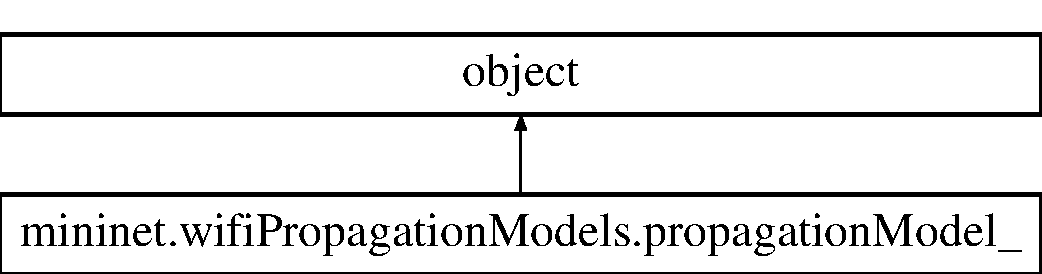
\includegraphics[height=2.000000cm]{classmininet_1_1wifiPropagationModels_1_1propagationModel__}
\end{center}
\end{figure}
\subsection*{Public Member Functions}
\begin{DoxyCompactItemize}
\item 
\hypertarget{classmininet_1_1wifiPropagationModels_1_1propagationModel___a6a47183b4f68353e3f22fada5c83e865}{def {\bfseries \-\_\-\-\_\-init\-\_\-\-\_\-}}\label{classmininet_1_1wifiPropagationModels_1_1propagationModel___a6a47183b4f68353e3f22fada5c83e865}

\item 
\hypertarget{classmininet_1_1wifiPropagationModels_1_1propagationModel___ac4ab2767db399b47f5c300c70e23d3d9}{def {\bfseries received\-Power}}\label{classmininet_1_1wifiPropagationModels_1_1propagationModel___ac4ab2767db399b47f5c300c70e23d3d9}

\item 
\hypertarget{classmininet_1_1wifiPropagationModels_1_1propagationModel___ab1eccb9c8767153d701bdbee7577ab23}{def {\bfseries attenuation}}\label{classmininet_1_1wifiPropagationModels_1_1propagationModel___ab1eccb9c8767153d701bdbee7577ab23}

\item 
def \hyperlink{classmininet_1_1wifiPropagationModels_1_1propagationModel___ac116895c706c4d9de59dfe1107b57c20}{friis\-Propagation\-Loss\-Model}
\item 
def \hyperlink{classmininet_1_1wifiPropagationModels_1_1propagationModel___a19fda68ddbddbf56131939aa7758b806}{two\-Ray\-Ground\-Propagation\-Loss\-Model}
\item 
def \hyperlink{classmininet_1_1wifiPropagationModels_1_1propagationModel___a85df966bcab9bb0475294fd71aeb1699}{log\-Distance\-Propagation\-Loss\-Model}
\item 
def \hyperlink{classmininet_1_1wifiPropagationModels_1_1propagationModel___a039a9b90d17295ffb41e116c7ea68e26}{okumura\-Hata\-Propagation\-Loss\-Model}
\item 
def \hyperlink{classmininet_1_1wifiPropagationModels_1_1propagationModel___a0af6ae4dac981d27c89eed916a1a1212}{jakes\-Propagation\-Loss\-Model}
\end{DoxyCompactItemize}
\subsection*{Public Attributes}
\begin{DoxyCompactItemize}
\item 
\hyperlink{classmininet_1_1wifiPropagationModels_1_1propagationModel___a5597e99932232cbe0e9879394c8055a3}{rssi}
\end{DoxyCompactItemize}
\subsection*{Static Public Attributes}
\begin{DoxyCompactItemize}
\item 
\hypertarget{classmininet_1_1wifiPropagationModels_1_1propagationModel___a0793e80d3e06a8d03bf856ad34d7ba71}{int {\bfseries rssi} = -\/62}\label{classmininet_1_1wifiPropagationModels_1_1propagationModel___a0793e80d3e06a8d03bf856ad34d7ba71}

\item 
\hypertarget{classmininet_1_1wifiPropagationModels_1_1propagationModel___a9a1266ab336f0f56e16960efc090dc6a}{string {\bfseries model} = ''}\label{classmininet_1_1wifiPropagationModels_1_1propagationModel___a9a1266ab336f0f56e16960efc090dc6a}

\item 
\hypertarget{classmininet_1_1wifiPropagationModels_1_1propagationModel___a9e272bfc2880eb20ffdf2f37f2f00e0d}{int {\bfseries exp} = 0}\label{classmininet_1_1wifiPropagationModels_1_1propagationModel___a9e272bfc2880eb20ffdf2f37f2f00e0d}

\item 
\hypertarget{classmininet_1_1wifiPropagationModels_1_1propagationModel___ab307987b99039365f8b1e0aff45f3516}{int {\bfseries sl} = 2}\label{classmininet_1_1wifiPropagationModels_1_1propagationModel___ab307987b99039365f8b1e0aff45f3516}

\end{DoxyCompactItemize}


\subsection{Detailed Description}
\begin{DoxyVerb}Propagation Models \end{DoxyVerb}
 

\subsection{Member Function Documentation}
\hypertarget{classmininet_1_1wifiPropagationModels_1_1propagationModel___ac116895c706c4d9de59dfe1107b57c20}{\index{mininet\-::wifi\-Propagation\-Models\-::propagation\-Model\-\_\-@{mininet\-::wifi\-Propagation\-Models\-::propagation\-Model\-\_\-}!friis\-Propagation\-Loss\-Model@{friis\-Propagation\-Loss\-Model}}
\index{friis\-Propagation\-Loss\-Model@{friis\-Propagation\-Loss\-Model}!mininet::wifiPropagationModels::propagationModel_@{mininet\-::wifi\-Propagation\-Models\-::propagation\-Model\-\_\-}}
\subsubsection[{friis\-Propagation\-Loss\-Model}]{\setlength{\rightskip}{0pt plus 5cm}def mininet.\-wifi\-Propagation\-Models.\-propagation\-Model\-\_\-.\-friis\-Propagation\-Loss\-Model (
\begin{DoxyParamCaption}
\item[{}]{self, }
\item[{}]{node1, }
\item[{}]{node2, }
\item[{}]{dist, }
\item[{}]{wlan}
\end{DoxyParamCaption}
)}}\label{classmininet_1_1wifiPropagationModels_1_1propagationModel___ac116895c706c4d9de59dfe1107b57c20}
\begin{DoxyVerb}Friis Propagation Loss Model:
(f) signal frequency transmited(Hz)
(d) is the distance between the transmitter and the receiver (m)
(c) speed of light in vacuum (m)
(L) System loss\end{DoxyVerb}
 \hypertarget{classmininet_1_1wifiPropagationModels_1_1propagationModel___a0af6ae4dac981d27c89eed916a1a1212}{\index{mininet\-::wifi\-Propagation\-Models\-::propagation\-Model\-\_\-@{mininet\-::wifi\-Propagation\-Models\-::propagation\-Model\-\_\-}!jakes\-Propagation\-Loss\-Model@{jakes\-Propagation\-Loss\-Model}}
\index{jakes\-Propagation\-Loss\-Model@{jakes\-Propagation\-Loss\-Model}!mininet::wifiPropagationModels::propagationModel_@{mininet\-::wifi\-Propagation\-Models\-::propagation\-Model\-\_\-}}
\subsubsection[{jakes\-Propagation\-Loss\-Model}]{\setlength{\rightskip}{0pt plus 5cm}def mininet.\-wifi\-Propagation\-Models.\-propagation\-Model\-\_\-.\-jakes\-Propagation\-Loss\-Model (
\begin{DoxyParamCaption}
\item[{}]{self, }
\item[{}]{node1, }
\item[{}]{node2, }
\item[{}]{distance, }
\item[{}]{wlan}
\end{DoxyParamCaption}
)}}\label{classmininet_1_1wifiPropagationModels_1_1propagationModel___a0af6ae4dac981d27c89eed916a1a1212}
\begin{DoxyVerb}Jakes Propagation Loss Model:\end{DoxyVerb}
 \hypertarget{classmininet_1_1wifiPropagationModels_1_1propagationModel___a85df966bcab9bb0475294fd71aeb1699}{\index{mininet\-::wifi\-Propagation\-Models\-::propagation\-Model\-\_\-@{mininet\-::wifi\-Propagation\-Models\-::propagation\-Model\-\_\-}!log\-Distance\-Propagation\-Loss\-Model@{log\-Distance\-Propagation\-Loss\-Model}}
\index{log\-Distance\-Propagation\-Loss\-Model@{log\-Distance\-Propagation\-Loss\-Model}!mininet::wifiPropagationModels::propagationModel_@{mininet\-::wifi\-Propagation\-Models\-::propagation\-Model\-\_\-}}
\subsubsection[{log\-Distance\-Propagation\-Loss\-Model}]{\setlength{\rightskip}{0pt plus 5cm}def mininet.\-wifi\-Propagation\-Models.\-propagation\-Model\-\_\-.\-log\-Distance\-Propagation\-Loss\-Model (
\begin{DoxyParamCaption}
\item[{}]{self, }
\item[{}]{node1, }
\item[{}]{node2, }
\item[{}]{dist, }
\item[{}]{wlan}
\end{DoxyParamCaption}
)}}\label{classmininet_1_1wifiPropagationModels_1_1propagationModel___a85df966bcab9bb0475294fd71aeb1699}
\begin{DoxyVerb}Log Distance Propagation Loss Model:
referenceDistance (m): The distance at which the reference loss is calculated
referenceLoss (db): The reference loss at reference distance. Default for 1m is 46.6777
exponent: The exponent of the Path Loss propagation model, where 2 is for propagation in free space
(d) is the distance between the transmitter and the receiver (m)\end{DoxyVerb}
 \hypertarget{classmininet_1_1wifiPropagationModels_1_1propagationModel___a039a9b90d17295ffb41e116c7ea68e26}{\index{mininet\-::wifi\-Propagation\-Models\-::propagation\-Model\-\_\-@{mininet\-::wifi\-Propagation\-Models\-::propagation\-Model\-\_\-}!okumura\-Hata\-Propagation\-Loss\-Model@{okumura\-Hata\-Propagation\-Loss\-Model}}
\index{okumura\-Hata\-Propagation\-Loss\-Model@{okumura\-Hata\-Propagation\-Loss\-Model}!mininet::wifiPropagationModels::propagationModel_@{mininet\-::wifi\-Propagation\-Models\-::propagation\-Model\-\_\-}}
\subsubsection[{okumura\-Hata\-Propagation\-Loss\-Model}]{\setlength{\rightskip}{0pt plus 5cm}def mininet.\-wifi\-Propagation\-Models.\-propagation\-Model\-\_\-.\-okumura\-Hata\-Propagation\-Loss\-Model (
\begin{DoxyParamCaption}
\item[{}]{self, }
\item[{}]{node1, }
\item[{}]{node2, }
\item[{}]{distance, }
\item[{}]{wlan}
\end{DoxyParamCaption}
)}}\label{classmininet_1_1wifiPropagationModels_1_1propagationModel___a039a9b90d17295ffb41e116c7ea68e26}
\begin{DoxyVerb}Okumura Hata Propagation Loss Model:\end{DoxyVerb}
 \hypertarget{classmininet_1_1wifiPropagationModels_1_1propagationModel___a19fda68ddbddbf56131939aa7758b806}{\index{mininet\-::wifi\-Propagation\-Models\-::propagation\-Model\-\_\-@{mininet\-::wifi\-Propagation\-Models\-::propagation\-Model\-\_\-}!two\-Ray\-Ground\-Propagation\-Loss\-Model@{two\-Ray\-Ground\-Propagation\-Loss\-Model}}
\index{two\-Ray\-Ground\-Propagation\-Loss\-Model@{two\-Ray\-Ground\-Propagation\-Loss\-Model}!mininet::wifiPropagationModels::propagationModel_@{mininet\-::wifi\-Propagation\-Models\-::propagation\-Model\-\_\-}}
\subsubsection[{two\-Ray\-Ground\-Propagation\-Loss\-Model}]{\setlength{\rightskip}{0pt plus 5cm}def mininet.\-wifi\-Propagation\-Models.\-propagation\-Model\-\_\-.\-two\-Ray\-Ground\-Propagation\-Loss\-Model (
\begin{DoxyParamCaption}
\item[{}]{self, }
\item[{}]{node1, }
\item[{}]{node2, }
\item[{}]{dist, }
\item[{}]{wlan}
\end{DoxyParamCaption}
)}}\label{classmininet_1_1wifiPropagationModels_1_1propagationModel___a19fda68ddbddbf56131939aa7758b806}
\begin{DoxyVerb}Two Ray Ground Propagation Loss Model:
(gT): Tx Antenna Gain (dBi)
(gR): Rx Antenna Gain (dBi)
(hT): Tx Antenna Height
(hR): Rx Antenna Height
(d) is the distance between the transmitter and the receiver (m)
(L): System loss\end{DoxyVerb}
 

\subsection{Member Data Documentation}
\hypertarget{classmininet_1_1wifiPropagationModels_1_1propagationModel___a5597e99932232cbe0e9879394c8055a3}{\index{mininet\-::wifi\-Propagation\-Models\-::propagation\-Model\-\_\-@{mininet\-::wifi\-Propagation\-Models\-::propagation\-Model\-\_\-}!rssi@{rssi}}
\index{rssi@{rssi}!mininet::wifiPropagationModels::propagationModel_@{mininet\-::wifi\-Propagation\-Models\-::propagation\-Model\-\_\-}}
\subsubsection[{rssi}]{\setlength{\rightskip}{0pt plus 5cm}mininet.\-wifi\-Propagation\-Models.\-propagation\-Model\-\_\-.\-rssi}}\label{classmininet_1_1wifiPropagationModels_1_1propagationModel___a5597e99932232cbe0e9879394c8055a3}
\begin{DoxyVerb}Two Ray Ground Propagation Loss Model:
(gT): Tx Antenna Gain (dBi)
(gR): Rx Antenna Gain (dBi)
(hT): Tx Antenna Height
(hR): Rx Antenna Height
(d) is the distance between the transmitter and the receiver (m)
(L): System loss\end{DoxyVerb}


\begin{DoxyVerb}Log Distance Propagation Loss Model:
referenceDistance (m): The distance at which the reference loss is calculated
referenceLoss (db): The reference loss at reference distance. Default for 1m is 46.6777
exponent: The exponent of the Path Loss propagation model, where 2 is for propagation in free space
(d) is the distance between the transmitter and the receiver (m)\end{DoxyVerb}
 

The documentation for this class was generated from the following file\-:\begin{DoxyCompactItemize}
\item 
wifi\-Propagation\-Models.\-py\end{DoxyCompactItemize}

\hypertarget{classmininet_1_1wifiMobilityModels_1_1RandomDirection}{\section{mininet.\-wifi\-Mobility\-Models.\-Random\-Direction Class Reference}
\label{classmininet_1_1wifiMobilityModels_1_1RandomDirection}\index{mininet.\-wifi\-Mobility\-Models.\-Random\-Direction@{mininet.\-wifi\-Mobility\-Models.\-Random\-Direction}}
}
Inheritance diagram for mininet.\-wifi\-Mobility\-Models.\-Random\-Direction\-:\begin{figure}[H]
\begin{center}
\leavevmode
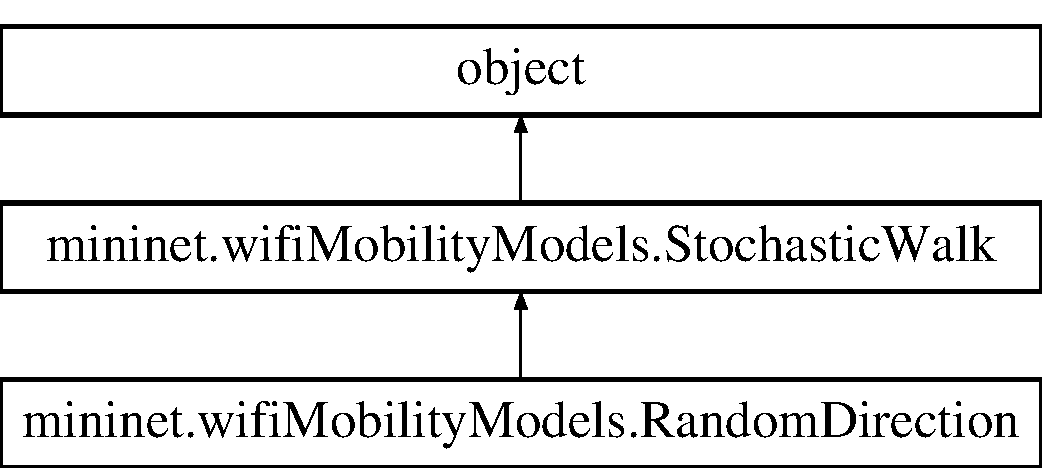
\includegraphics[height=3.000000cm]{classmininet_1_1wifiMobilityModels_1_1RandomDirection}
\end{center}
\end{figure}
\subsection*{Public Member Functions}
\begin{DoxyCompactItemize}
\item 
def \hyperlink{classmininet_1_1wifiMobilityModels_1_1RandomDirection_af539c766498fe00c98abf6c2de913498}{\-\_\-\-\_\-init\-\_\-\-\_\-}
\end{DoxyCompactItemize}
\subsection*{Additional Inherited Members}


\subsection{Constructor \& Destructor Documentation}
\hypertarget{classmininet_1_1wifiMobilityModels_1_1RandomDirection_af539c766498fe00c98abf6c2de913498}{\index{mininet\-::wifi\-Mobility\-Models\-::\-Random\-Direction@{mininet\-::wifi\-Mobility\-Models\-::\-Random\-Direction}!\-\_\-\-\_\-init\-\_\-\-\_\-@{\-\_\-\-\_\-init\-\_\-\-\_\-}}
\index{\-\_\-\-\_\-init\-\_\-\-\_\-@{\-\_\-\-\_\-init\-\_\-\-\_\-}!mininet::wifiMobilityModels::RandomDirection@{mininet\-::wifi\-Mobility\-Models\-::\-Random\-Direction}}
\subsubsection[{\-\_\-\-\_\-init\-\_\-\-\_\-}]{\setlength{\rightskip}{0pt plus 5cm}def mininet.\-wifi\-Mobility\-Models.\-Random\-Direction.\-\_\-\-\_\-init\-\_\-\-\_\- (
\begin{DoxyParamCaption}
\item[{}]{self, }
\item[{}]{nr\-\_\-nodes, }
\item[{}]{dimensions, }
\item[{}]{wt\-\_\-max = {\ttfamily None}, }
\item[{}]{velocity = {\ttfamily (0.1,~1.}, }
\item[{}]{border\-\_\-policy = {\ttfamily 'reflect'}}
\end{DoxyParamCaption}
)}}\label{classmininet_1_1wifiMobilityModels_1_1RandomDirection_af539c766498fe00c98abf6c2de913498}
\begin{DoxyVerb}Random Direction mobility model.
This model is based in the Stochastic Walk. The flight length is chosen from a uniform distribution, 
with minimum 0 and maximum set to the maximum dimension value.
The velocity is also chosen from a uniform distribution, with boundaries set by the *velocity* parameter.
If wt_max is set, the waiting time is chosen from a uniform distribution with values between 0 and wt_max.
If wt_max is not set, waiting time is set to None.

Required arguments:

  *nr_nodes*:
    Integer, the number of nodes.
  
  *dimensions*:
    Tuple of Integers, the x and y dimensions of the simulation area.
  
keyword arguments:

  *wt_max*:
    Double, maximum value for the waiting time distribution.
    If wt_max is set, the waiting time is chosen from a uniform distribution with values between 0 and wt_max.
    If wt_max is not set, the waiting time is set to None.
    Default is None.
  
  *velocity*:
    Tuple of Doubles, the minimum and maximum values for node velocity.
    
  *border_policy*:
    String, either 'reflect' or 'wrap'. The policy that is used when the node arrives to the border.
    If 'reflect', the node reflects off the border.
    If 'wrap', the node reappears at the opposite edge (as in a torus-shaped area).
\end{DoxyVerb}
 

The documentation for this class was generated from the following file\-:\begin{DoxyCompactItemize}
\item 
wifi\-Mobility\-Models.\-py\end{DoxyCompactItemize}

\hypertarget{classmininet_1_1wifiMobilityModels_1_1RandomWalk}{\section{mininet.\-wifi\-Mobility\-Models.\-Random\-Walk Class Reference}
\label{classmininet_1_1wifiMobilityModels_1_1RandomWalk}\index{mininet.\-wifi\-Mobility\-Models.\-Random\-Walk@{mininet.\-wifi\-Mobility\-Models.\-Random\-Walk}}
}
Inheritance diagram for mininet.\-wifi\-Mobility\-Models.\-Random\-Walk\-:\begin{figure}[H]
\begin{center}
\leavevmode
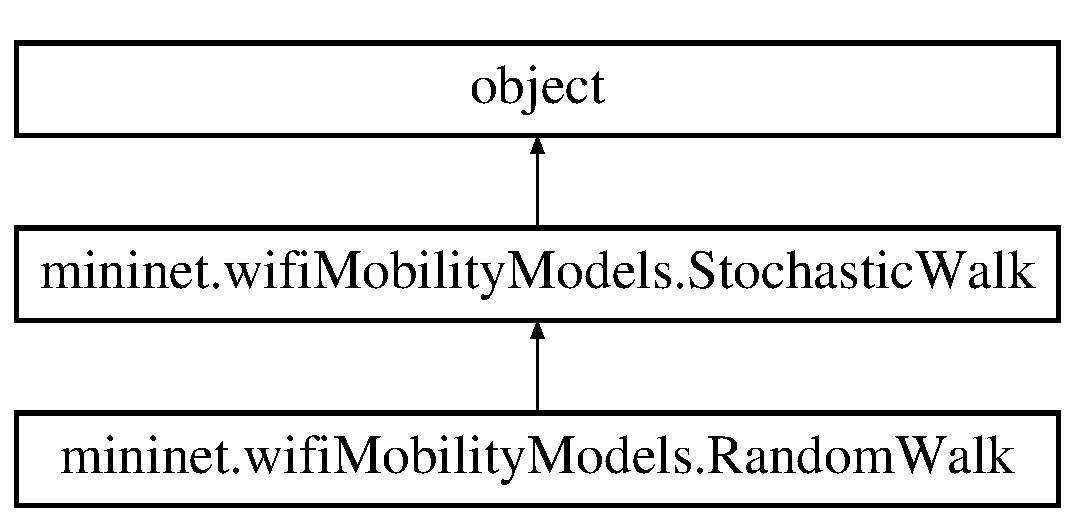
\includegraphics[height=3.000000cm]{classmininet_1_1wifiMobilityModels_1_1RandomWalk}
\end{center}
\end{figure}
\subsection*{Public Member Functions}
\begin{DoxyCompactItemize}
\item 
def \hyperlink{classmininet_1_1wifiMobilityModels_1_1RandomWalk_ae3af0b58f0622e21bcb5f427387ddca1}{\-\_\-\-\_\-init\-\_\-\-\_\-}
\end{DoxyCompactItemize}
\subsection*{Additional Inherited Members}


\subsection{Constructor \& Destructor Documentation}
\hypertarget{classmininet_1_1wifiMobilityModels_1_1RandomWalk_ae3af0b58f0622e21bcb5f427387ddca1}{\index{mininet\-::wifi\-Mobility\-Models\-::\-Random\-Walk@{mininet\-::wifi\-Mobility\-Models\-::\-Random\-Walk}!\-\_\-\-\_\-init\-\_\-\-\_\-@{\-\_\-\-\_\-init\-\_\-\-\_\-}}
\index{\-\_\-\-\_\-init\-\_\-\-\_\-@{\-\_\-\-\_\-init\-\_\-\-\_\-}!mininet::wifiMobilityModels::RandomWalk@{mininet\-::wifi\-Mobility\-Models\-::\-Random\-Walk}}
\subsubsection[{\-\_\-\-\_\-init\-\_\-\-\_\-}]{\setlength{\rightskip}{0pt plus 5cm}def mininet.\-wifi\-Mobility\-Models.\-Random\-Walk.\-\_\-\-\_\-init\-\_\-\-\_\- (
\begin{DoxyParamCaption}
\item[{}]{self, }
\item[{}]{nr\-\_\-nodes, }
\item[{}]{dimensions, }
\item[{}]{velocity = {\ttfamily 1.}, }
\item[{}]{distance = {\ttfamily 1.}, }
\item[{}]{border\-\_\-policy = {\ttfamily 'reflect'}}
\end{DoxyParamCaption}
)}}\label{classmininet_1_1wifiMobilityModels_1_1RandomWalk_ae3af0b58f0622e21bcb5f427387ddca1}
\begin{DoxyVerb}Random Walk mobility model.
This model is based in the Stochastic Walk, but both the flight length and node velocity distributions are in fact constants,
set to the *distance* and *velocity* parameters. The waiting time is set to None.

Required arguments:

  *nr_nodes*:
    Integer, the number of nodes.
  
  *dimensions*:
    Tuple of Integers, the x and y dimensions of the simulation area.
  
keyword arguments:

  *velocity*:
    Double, the value for the constant node velocity. Default is 1.0
  
  *distance*:
    Double, the value for the constant distance traveled in each step. Default is 1.0
    
  *border_policy*:
    String, either 'reflect' or 'wrap'. The policy that is used when the node arrives to the border.
    If 'reflect', the node reflects off the border.
    If 'wrap', the node reappears at the opposite edge (as in a torus-shaped area).
\end{DoxyVerb}
 

The documentation for this class was generated from the following file\-:\begin{DoxyCompactItemize}
\item 
wifi\-Mobility\-Models.\-py\end{DoxyCompactItemize}

\hypertarget{classmininet_1_1wifiMobilityModels_1_1RandomWaypoint}{\section{mininet.\-wifi\-Mobility\-Models.\-Random\-Waypoint Class Reference}
\label{classmininet_1_1wifiMobilityModels_1_1RandomWaypoint}\index{mininet.\-wifi\-Mobility\-Models.\-Random\-Waypoint@{mininet.\-wifi\-Mobility\-Models.\-Random\-Waypoint}}
}
Inheritance diagram for mininet.\-wifi\-Mobility\-Models.\-Random\-Waypoint\-:\begin{figure}[H]
\begin{center}
\leavevmode
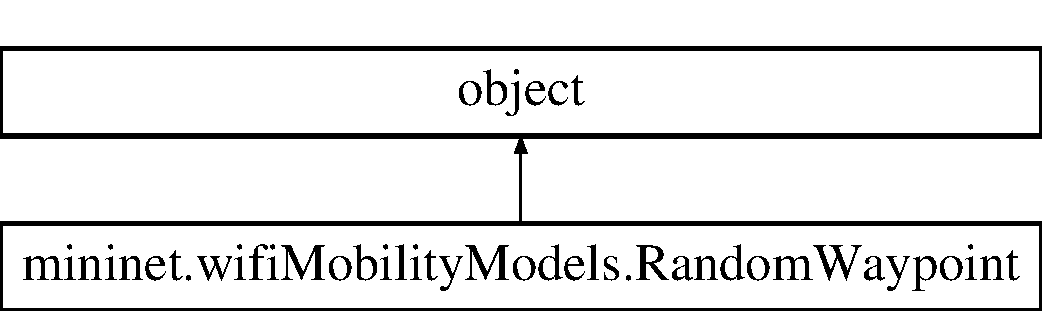
\includegraphics[height=2.000000cm]{classmininet_1_1wifiMobilityModels_1_1RandomWaypoint}
\end{center}
\end{figure}
\subsection*{Public Member Functions}
\begin{DoxyCompactItemize}
\item 
def \hyperlink{classmininet_1_1wifiMobilityModels_1_1RandomWaypoint_ac1ac4b60d2dbca916ebd2f1793cf05d9}{\-\_\-\-\_\-init\-\_\-\-\_\-}
\item 
\hypertarget{classmininet_1_1wifiMobilityModels_1_1RandomWaypoint_a01f5d4017bc5d4c557ecc5e1bda071e6}{def {\bfseries \-\_\-\-\_\-iter\-\_\-\-\_\-}}\label{classmininet_1_1wifiMobilityModels_1_1RandomWaypoint_a01f5d4017bc5d4c557ecc5e1bda071e6}

\end{DoxyCompactItemize}
\subsection*{Public Attributes}
\begin{DoxyCompactItemize}
\item 
\hypertarget{classmininet_1_1wifiMobilityModels_1_1RandomWaypoint_a90ab333a2f2ce355661ec1f9f3a7a31f}{{\bfseries nr\-\_\-nodes}}\label{classmininet_1_1wifiMobilityModels_1_1RandomWaypoint_a90ab333a2f2ce355661ec1f9f3a7a31f}

\item 
\hypertarget{classmininet_1_1wifiMobilityModels_1_1RandomWaypoint_a720b9b6226d9e6b0356c0b3a7614e866}{{\bfseries dimensions}}\label{classmininet_1_1wifiMobilityModels_1_1RandomWaypoint_a720b9b6226d9e6b0356c0b3a7614e866}

\item 
\hypertarget{classmininet_1_1wifiMobilityModels_1_1RandomWaypoint_a7a7c4eef3cb4f74c78db48b4ba92c47a}{{\bfseries velocity}}\label{classmininet_1_1wifiMobilityModels_1_1RandomWaypoint_a7a7c4eef3cb4f74c78db48b4ba92c47a}

\item 
\hypertarget{classmininet_1_1wifiMobilityModels_1_1RandomWaypoint_a90284d9c64bf4b160c79b8d6648806ca}{{\bfseries wt\-\_\-max}}\label{classmininet_1_1wifiMobilityModels_1_1RandomWaypoint_a90284d9c64bf4b160c79b8d6648806ca}

\item 
\hypertarget{classmininet_1_1wifiMobilityModels_1_1RandomWaypoint_afa5f276b232144d9e8dd9d029077f910}{{\bfseries init\-\_\-stationary}}\label{classmininet_1_1wifiMobilityModels_1_1RandomWaypoint_afa5f276b232144d9e8dd9d029077f910}

\item 
\hypertarget{classmininet_1_1wifiMobilityModels_1_1RandomWaypoint_a9fb7abe39aafbe5626f634d7615bfaf2}{{\bfseries wt}}\label{classmininet_1_1wifiMobilityModels_1_1RandomWaypoint_a9fb7abe39aafbe5626f634d7615bfaf2}

\end{DoxyCompactItemize}


\subsection{Constructor \& Destructor Documentation}
\hypertarget{classmininet_1_1wifiMobilityModels_1_1RandomWaypoint_ac1ac4b60d2dbca916ebd2f1793cf05d9}{\index{mininet\-::wifi\-Mobility\-Models\-::\-Random\-Waypoint@{mininet\-::wifi\-Mobility\-Models\-::\-Random\-Waypoint}!\-\_\-\-\_\-init\-\_\-\-\_\-@{\-\_\-\-\_\-init\-\_\-\-\_\-}}
\index{\-\_\-\-\_\-init\-\_\-\-\_\-@{\-\_\-\-\_\-init\-\_\-\-\_\-}!mininet::wifiMobilityModels::RandomWaypoint@{mininet\-::wifi\-Mobility\-Models\-::\-Random\-Waypoint}}
\subsubsection[{\-\_\-\-\_\-init\-\_\-\-\_\-}]{\setlength{\rightskip}{0pt plus 5cm}def mininet.\-wifi\-Mobility\-Models.\-Random\-Waypoint.\-\_\-\-\_\-init\-\_\-\-\_\- (
\begin{DoxyParamCaption}
\item[{}]{self, }
\item[{}]{nr\-\_\-nodes, }
\item[{}]{dimensions, }
\item[{}]{velocity = {\ttfamily (0.1,~1.}, }
\item[{}]{wt\-\_\-max = {\ttfamily None}}
\end{DoxyParamCaption}
)}}\label{classmininet_1_1wifiMobilityModels_1_1RandomWaypoint_ac1ac4b60d2dbca916ebd2f1793cf05d9}
\begin{DoxyVerb}Random Waypoint model.

Required arguments:

  *nr_nodes*:
    Integer, the number of nodes.
  
  *dimensions*:
    Tuple of Integers, the x and y dimensions of the simulation area.
  
keyword arguments:

  *velocity*:
    Tuple of Integers, the minimum and maximum values for node velocity.
  
  *wt_max*:
    Integer, the maximum wait time for node pauses.
    If wt_max is 0 or None, there is no pause time.
\end{DoxyVerb}
 

The documentation for this class was generated from the following file\-:\begin{DoxyCompactItemize}
\item 
wifi\-Mobility\-Models.\-py\end{DoxyCompactItemize}

\hypertarget{classmininet_1_1node_1_1RemoteController}{\section{mininet.\-node.\-Remote\-Controller Class Reference}
\label{classmininet_1_1node_1_1RemoteController}\index{mininet.\-node.\-Remote\-Controller@{mininet.\-node.\-Remote\-Controller}}
}
Inheritance diagram for mininet.\-node.\-Remote\-Controller\-:\begin{figure}[H]
\begin{center}
\leavevmode
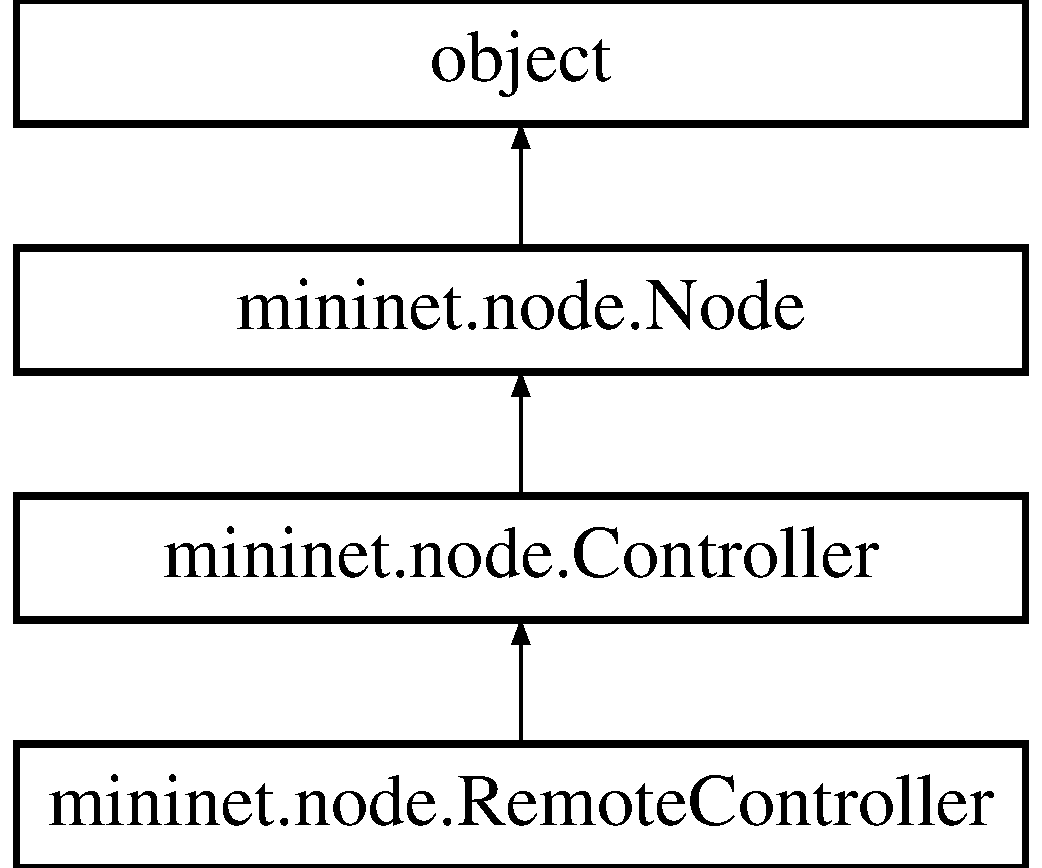
\includegraphics[height=4.000000cm]{classmininet_1_1node_1_1RemoteController}
\end{center}
\end{figure}
\subsection*{Public Member Functions}
\begin{DoxyCompactItemize}
\item 
def \hyperlink{classmininet_1_1node_1_1RemoteController_a132ade806efe16afd8378b6b3d8603ef}{\-\_\-\-\_\-init\-\_\-\-\_\-}
\item 
\hypertarget{classmininet_1_1node_1_1RemoteController_af04ce96293cdef74e7e3acfc1060c312}{def {\bfseries start}}\label{classmininet_1_1node_1_1RemoteController_af04ce96293cdef74e7e3acfc1060c312}

\item 
\hypertarget{classmininet_1_1node_1_1RemoteController_a423cd2c18743a69404d6a793f004dd8b}{def {\bfseries stop}}\label{classmininet_1_1node_1_1RemoteController_a423cd2c18743a69404d6a793f004dd8b}

\item 
\hypertarget{classmininet_1_1node_1_1RemoteController_a5fc4f5ec3d96e159b60f8668b880bc93}{def {\bfseries check\-Listening}}\label{classmininet_1_1node_1_1RemoteController_a5fc4f5ec3d96e159b60f8668b880bc93}

\item 
\hypertarget{classmininet_1_1node_1_1RemoteController_aee6882c7ea0a5240022526857f25e0a6}{def {\bfseries is\-Listening}}\label{classmininet_1_1node_1_1RemoteController_aee6882c7ea0a5240022526857f25e0a6}

\end{DoxyCompactItemize}
\subsection*{Public Attributes}
\begin{DoxyCompactItemize}
\item 
\hypertarget{classmininet_1_1node_1_1RemoteController_a828931b06ff374c712c345ca14ed841c}{{\bfseries port}}\label{classmininet_1_1node_1_1RemoteController_a828931b06ff374c712c345ca14ed841c}

\end{DoxyCompactItemize}
\subsection*{Additional Inherited Members}


\subsection{Constructor \& Destructor Documentation}
\hypertarget{classmininet_1_1node_1_1RemoteController_a132ade806efe16afd8378b6b3d8603ef}{\index{mininet\-::node\-::\-Remote\-Controller@{mininet\-::node\-::\-Remote\-Controller}!\-\_\-\-\_\-init\-\_\-\-\_\-@{\-\_\-\-\_\-init\-\_\-\-\_\-}}
\index{\-\_\-\-\_\-init\-\_\-\-\_\-@{\-\_\-\-\_\-init\-\_\-\-\_\-}!mininet::node::RemoteController@{mininet\-::node\-::\-Remote\-Controller}}
\subsubsection[{\-\_\-\-\_\-init\-\_\-\-\_\-}]{\setlength{\rightskip}{0pt plus 5cm}def mininet.\-node.\-Remote\-Controller.\-\_\-\-\_\-init\-\_\-\-\_\- (
\begin{DoxyParamCaption}
\item[{}]{self, }
\item[{}]{name, }
\item[{}]{ip = {\ttfamily '127.0.0.1'}, }
\item[{}]{port = {\ttfamily None}, }
\item[{}]{kwargs}
\end{DoxyParamCaption}
)}}\label{classmininet_1_1node_1_1RemoteController_a132ade806efe16afd8378b6b3d8603ef}
\begin{DoxyVerb}Init.
   name: name to give controller
   ip: the IP address where the remote controller is
   listening
   port: the port where the remote controller is listening\end{DoxyVerb}
 

The documentation for this class was generated from the following file\-:\begin{DoxyCompactItemize}
\item 
node.\-py\end{DoxyCompactItemize}

\hypertarget{classmininet_1_1wifiReport_1_1report}{\section{mininet.\-wifi\-Report.\-report Class Reference}
\label{classmininet_1_1wifiReport_1_1report}\index{mininet.\-wifi\-Report.\-report@{mininet.\-wifi\-Report.\-report}}
}
Inheritance diagram for mininet.\-wifi\-Report.\-report\-:\begin{figure}[H]
\begin{center}
\leavevmode
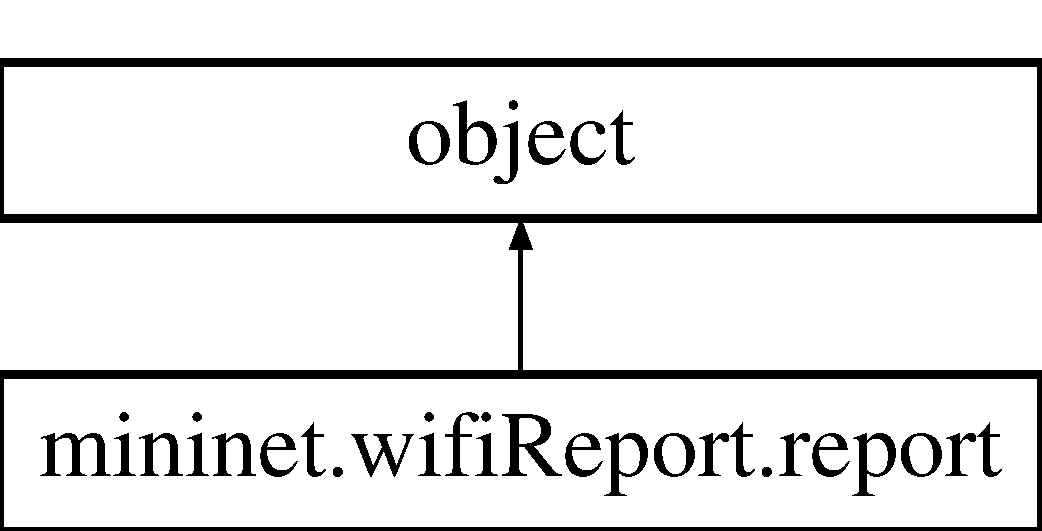
\includegraphics[height=2.000000cm]{classmininet_1_1wifiReport_1_1report}
\end{center}
\end{figure}
\subsection*{Public Member Functions}
\begin{DoxyCompactItemize}
\item 
\hypertarget{classmininet_1_1wifiReport_1_1report_ae922c90cd2693336092369c3b2c5a7e6}{def {\bfseries \-\_\-\-\_\-init\-\_\-\-\_\-}}\label{classmininet_1_1wifiReport_1_1report_ae922c90cd2693336092369c3b2c5a7e6}

\item 
\hypertarget{classmininet_1_1wifiReport_1_1report_a182090f7b1e9a332d4fcd1c7d049bd70}{def {\bfseries start}}\label{classmininet_1_1wifiReport_1_1report_a182090f7b1e9a332d4fcd1c7d049bd70}

\end{DoxyCompactItemize}
\subsection*{Public Attributes}
\begin{DoxyCompactItemize}
\item 
\hypertarget{classmininet_1_1wifiReport_1_1report_a4236a1187ed3b7d5ba3a8c485edda259}{{\bfseries thread}}\label{classmininet_1_1wifiReport_1_1report_a4236a1187ed3b7d5ba3a8c485edda259}

\item 
\hypertarget{classmininet_1_1wifiReport_1_1report_a7db6127b8070248931777d9d18ecd6a6}{{\bfseries dist}}\label{classmininet_1_1wifiReport_1_1report_a7db6127b8070248931777d9d18ecd6a6}

\end{DoxyCompactItemize}
\subsection*{Static Public Attributes}
\begin{DoxyCompactItemize}
\item 
\hypertarget{classmininet_1_1wifiReport_1_1report_ab9285db73d7f4761b2c7365b3a9068f0}{int {\bfseries rssi} = -\/62}\label{classmininet_1_1wifiReport_1_1report_ab9285db73d7f4761b2c7365b3a9068f0}

\item 
\hypertarget{classmininet_1_1wifiReport_1_1report_a67ef3ed12777e72f85552b8f485419ae}{int {\bfseries dist} = 0}\label{classmininet_1_1wifiReport_1_1report_a67ef3ed12777e72f85552b8f485419ae}

\end{DoxyCompactItemize}


\subsection{Detailed Description}
\begin{DoxyVerb}Propagation Models \end{DoxyVerb}
 

The documentation for this class was generated from the following file\-:\begin{DoxyCompactItemize}
\item 
wifi\-Report.\-py\end{DoxyCompactItemize}

\hypertarget{classmininet_1_1node_1_1Ryu}{\section{mininet.\-node.\-Ryu Class Reference}
\label{classmininet_1_1node_1_1Ryu}\index{mininet.\-node.\-Ryu@{mininet.\-node.\-Ryu}}
}
Inheritance diagram for mininet.\-node.\-Ryu\-:\begin{figure}[H]
\begin{center}
\leavevmode
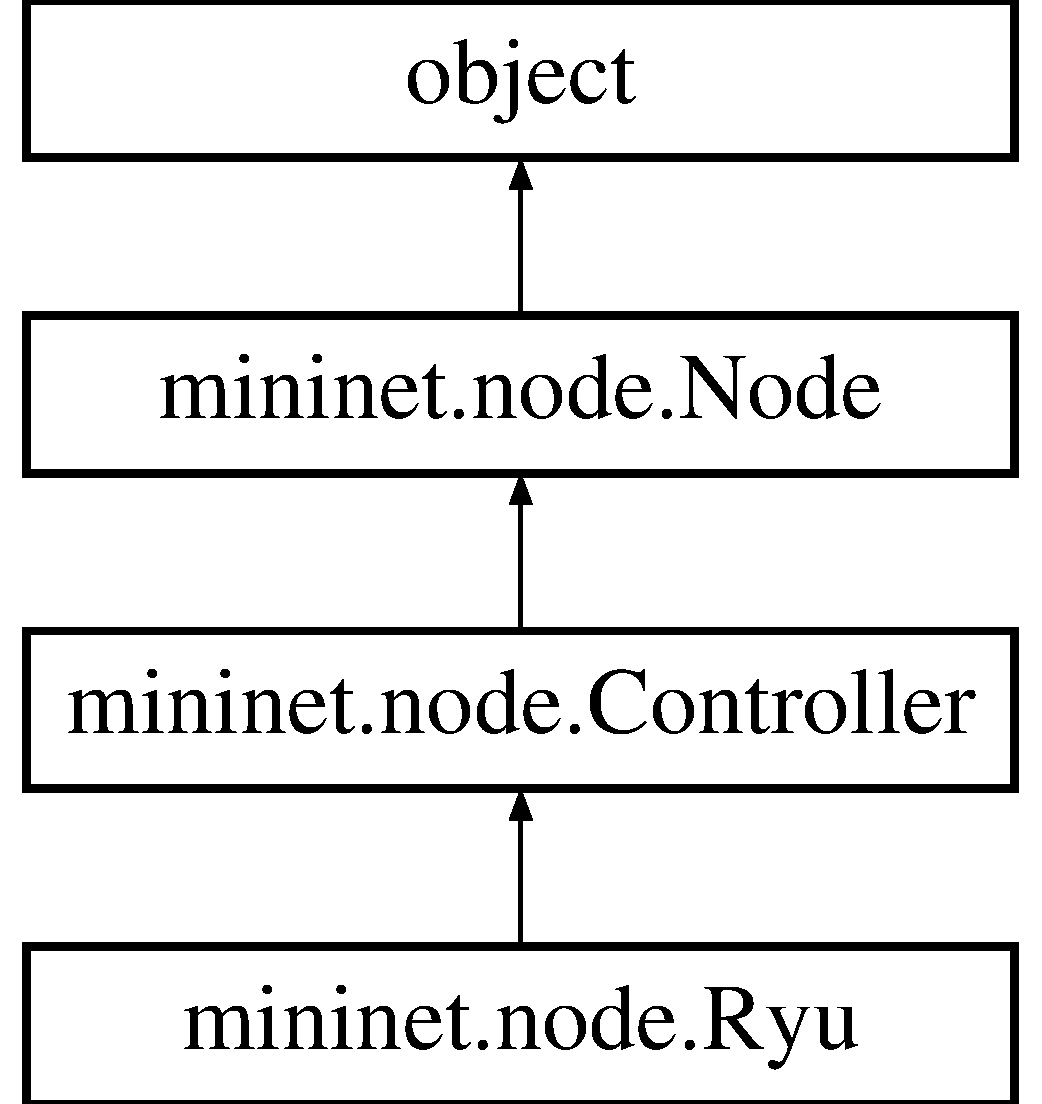
\includegraphics[height=4.000000cm]{classmininet_1_1node_1_1Ryu}
\end{center}
\end{figure}
\subsection*{Public Member Functions}
\begin{DoxyCompactItemize}
\item 
def \hyperlink{classmininet_1_1node_1_1Ryu_a1b0c45c79eb6c4d0a886f3e0e8cd52a5}{\-\_\-\-\_\-init\-\_\-\-\_\-}
\end{DoxyCompactItemize}
\subsection*{Additional Inherited Members}


\subsection{Constructor \& Destructor Documentation}
\hypertarget{classmininet_1_1node_1_1Ryu_a1b0c45c79eb6c4d0a886f3e0e8cd52a5}{\index{mininet\-::node\-::\-Ryu@{mininet\-::node\-::\-Ryu}!\-\_\-\-\_\-init\-\_\-\-\_\-@{\-\_\-\-\_\-init\-\_\-\-\_\-}}
\index{\-\_\-\-\_\-init\-\_\-\-\_\-@{\-\_\-\-\_\-init\-\_\-\-\_\-}!mininet::node::Ryu@{mininet\-::node\-::\-Ryu}}
\subsubsection[{\-\_\-\-\_\-init\-\_\-\-\_\-}]{\setlength{\rightskip}{0pt plus 5cm}def mininet.\-node.\-Ryu.\-\_\-\-\_\-init\-\_\-\-\_\- (
\begin{DoxyParamCaption}
\item[{}]{self, }
\item[{}]{name, }
\item[{}]{ryu\-Args, }
\item[{}]{kwargs}
\end{DoxyParamCaption}
)}}\label{classmininet_1_1node_1_1Ryu_a1b0c45c79eb6c4d0a886f3e0e8cd52a5}
\begin{DoxyVerb}Init.
name: name to give controller.
ryuArgs: arguments and modules to pass to Ryu\end{DoxyVerb}
 

The documentation for this class was generated from the following file\-:\begin{DoxyCompactItemize}
\item 
node.\-py\end{DoxyCompactItemize}

\hypertarget{classmininet_1_1topo_1_1SingleSwitchReversedTopo}{\section{mininet.\-topo.\-Single\-Switch\-Reversed\-Topo Class Reference}
\label{classmininet_1_1topo_1_1SingleSwitchReversedTopo}\index{mininet.\-topo.\-Single\-Switch\-Reversed\-Topo@{mininet.\-topo.\-Single\-Switch\-Reversed\-Topo}}
}
Inheritance diagram for mininet.\-topo.\-Single\-Switch\-Reversed\-Topo\-:\begin{figure}[H]
\begin{center}
\leavevmode
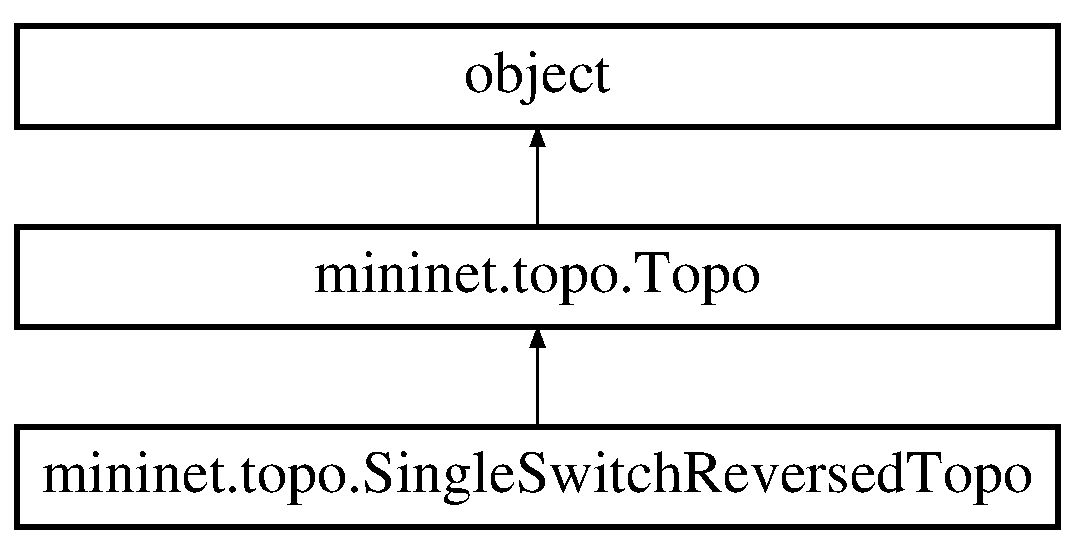
\includegraphics[height=3.000000cm]{classmininet_1_1topo_1_1SingleSwitchReversedTopo}
\end{center}
\end{figure}
\subsection*{Public Member Functions}
\begin{DoxyCompactItemize}
\item 
\hypertarget{classmininet_1_1topo_1_1SingleSwitchReversedTopo_a5c36c11d157b32993458c40ca8acca3d}{def {\bfseries build}}\label{classmininet_1_1topo_1_1SingleSwitchReversedTopo_a5c36c11d157b32993458c40ca8acca3d}

\end{DoxyCompactItemize}
\subsection*{Public Attributes}
\begin{DoxyCompactItemize}
\item 
\hypertarget{classmininet_1_1topo_1_1SingleSwitchReversedTopo_a21e1290c70d844b13bbcc50d5939b8f2}{{\bfseries k}}\label{classmininet_1_1topo_1_1SingleSwitchReversedTopo_a21e1290c70d844b13bbcc50d5939b8f2}

\end{DoxyCompactItemize}
\subsection*{Additional Inherited Members}


\subsection{Detailed Description}
\begin{DoxyVerb}Single switch connected to k hosts, with reversed ports.
   The lowest-numbered host is connected to the highest-numbered port.
   Useful to verify that Mininet properly handles custom port
   numberings.\end{DoxyVerb}
 

The documentation for this class was generated from the following file\-:\begin{DoxyCompactItemize}
\item 
topo.\-py\end{DoxyCompactItemize}

\hypertarget{classmininet_1_1topo_1_1SingleSwitchTopo}{\section{mininet.\-topo.\-Single\-Switch\-Topo Class Reference}
\label{classmininet_1_1topo_1_1SingleSwitchTopo}\index{mininet.\-topo.\-Single\-Switch\-Topo@{mininet.\-topo.\-Single\-Switch\-Topo}}
}
Inheritance diagram for mininet.\-topo.\-Single\-Switch\-Topo\-:\begin{figure}[H]
\begin{center}
\leavevmode
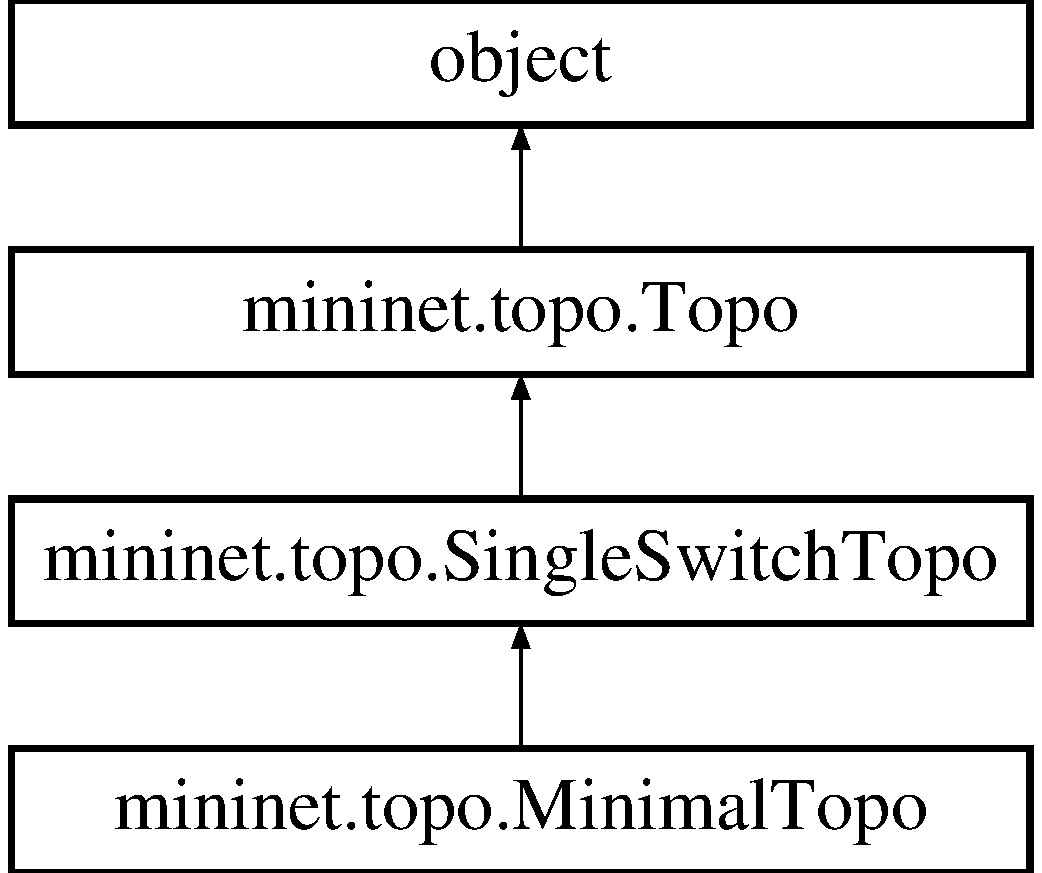
\includegraphics[height=4.000000cm]{classmininet_1_1topo_1_1SingleSwitchTopo}
\end{center}
\end{figure}
\subsection*{Public Member Functions}
\begin{DoxyCompactItemize}
\item 
\hypertarget{classmininet_1_1topo_1_1SingleSwitchTopo_a0b1bf95d0acf7350e732d74a01b1bbf0}{def {\bfseries build}}\label{classmininet_1_1topo_1_1SingleSwitchTopo_a0b1bf95d0acf7350e732d74a01b1bbf0}

\end{DoxyCompactItemize}
\subsection*{Public Attributes}
\begin{DoxyCompactItemize}
\item 
\hypertarget{classmininet_1_1topo_1_1SingleSwitchTopo_ad6f6c3126fe3c129a6b2ab2b8f1714d8}{{\bfseries k}}\label{classmininet_1_1topo_1_1SingleSwitchTopo_ad6f6c3126fe3c129a6b2ab2b8f1714d8}

\end{DoxyCompactItemize}
\subsection*{Additional Inherited Members}


The documentation for this class was generated from the following file\-:\begin{DoxyCompactItemize}
\item 
topo.\-py\end{DoxyCompactItemize}

\hypertarget{classmininet_1_1log_1_1Singleton}{\section{mininet.\-log.\-Singleton Class Reference}
\label{classmininet_1_1log_1_1Singleton}\index{mininet.\-log.\-Singleton@{mininet.\-log.\-Singleton}}
}
Inheritance diagram for mininet.\-log.\-Singleton\-:\begin{figure}[H]
\begin{center}
\leavevmode
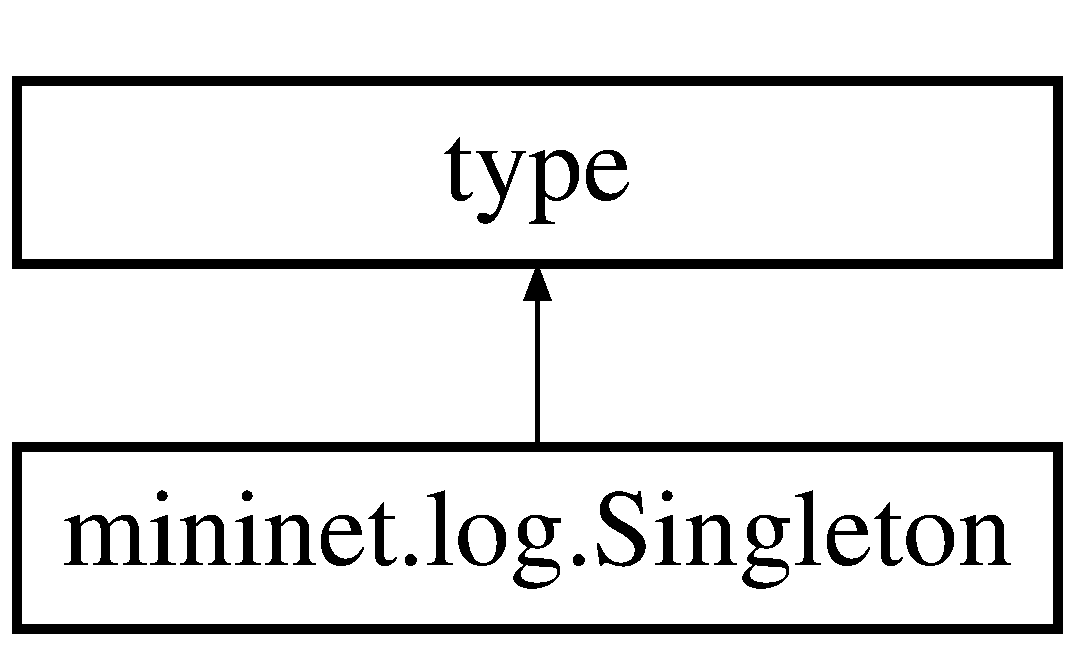
\includegraphics[height=2.000000cm]{classmininet_1_1log_1_1Singleton}
\end{center}
\end{figure}
\subsection*{Public Member Functions}
\begin{DoxyCompactItemize}
\item 
\hypertarget{classmininet_1_1log_1_1Singleton_a1a68c868c4b2465d47208f399e765fbe}{def {\bfseries \-\_\-\-\_\-init\-\_\-\-\_\-}}\label{classmininet_1_1log_1_1Singleton_a1a68c868c4b2465d47208f399e765fbe}

\item 
\hypertarget{classmininet_1_1log_1_1Singleton_a418a365d5ff47e3ff0362350716b461f}{def {\bfseries \-\_\-\-\_\-call\-\_\-\-\_\-}}\label{classmininet_1_1log_1_1Singleton_a418a365d5ff47e3ff0362350716b461f}

\end{DoxyCompactItemize}


\subsection{Detailed Description}
\begin{DoxyVerb}Singleton pattern from Wikipedia
   See http://en.wikipedia.org/wiki/Singleton_Pattern

   Intended to be used as a __metaclass_ param, as shown for the class
   below.\end{DoxyVerb}
 

The documentation for this class was generated from the following file\-:\begin{DoxyCompactItemize}
\item 
log.\-py\end{DoxyCompactItemize}

\hypertarget{classmininet_1_1wifiMobilityModels_1_1StochasticWalk}{\section{mininet.\-wifi\-Mobility\-Models.\-Stochastic\-Walk Class Reference}
\label{classmininet_1_1wifiMobilityModels_1_1StochasticWalk}\index{mininet.\-wifi\-Mobility\-Models.\-Stochastic\-Walk@{mininet.\-wifi\-Mobility\-Models.\-Stochastic\-Walk}}
}
Inheritance diagram for mininet.\-wifi\-Mobility\-Models.\-Stochastic\-Walk\-:\begin{figure}[H]
\begin{center}
\leavevmode
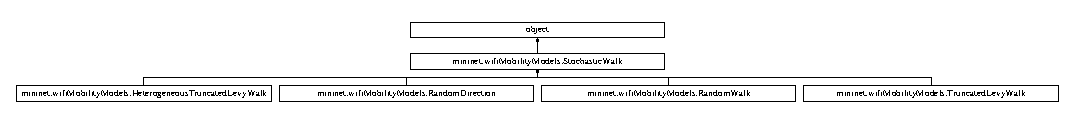
\includegraphics[height=1.138211cm]{classmininet_1_1wifiMobilityModels_1_1StochasticWalk}
\end{center}
\end{figure}
\subsection*{Public Member Functions}
\begin{DoxyCompactItemize}
\item 
def \hyperlink{classmininet_1_1wifiMobilityModels_1_1StochasticWalk_a2fc5338be6b275bc332d68c674900bd0}{\-\_\-\-\_\-init\-\_\-\-\_\-}
\item 
\hypertarget{classmininet_1_1wifiMobilityModels_1_1StochasticWalk_a354a1d28f552cd04a0537f64dbf262e5}{def {\bfseries \-\_\-\-\_\-iter\-\_\-\-\_\-}}\label{classmininet_1_1wifiMobilityModels_1_1StochasticWalk_a354a1d28f552cd04a0537f64dbf262e5}

\end{DoxyCompactItemize}
\subsection*{Public Attributes}
\begin{DoxyCompactItemize}
\item 
\hypertarget{classmininet_1_1wifiMobilityModels_1_1StochasticWalk_a8b4ae8718f4bca60a16f1879f8245fca}{{\bfseries collect\-\_\-fl\-\_\-stats}}\label{classmininet_1_1wifiMobilityModels_1_1StochasticWalk_a8b4ae8718f4bca60a16f1879f8245fca}

\item 
\hypertarget{classmininet_1_1wifiMobilityModels_1_1StochasticWalk_a1733fca42d6fa3905d850889dc512b3f}{{\bfseries collect\-\_\-wt\-\_\-stats}}\label{classmininet_1_1wifiMobilityModels_1_1StochasticWalk_a1733fca42d6fa3905d850889dc512b3f}

\item 
\hypertarget{classmininet_1_1wifiMobilityModels_1_1StochasticWalk_a3ca316e7b8d7986e9af94ebce3ae4b9c}{{\bfseries border\-\_\-policy}}\label{classmininet_1_1wifiMobilityModels_1_1StochasticWalk_a3ca316e7b8d7986e9af94ebce3ae4b9c}

\item 
\hypertarget{classmininet_1_1wifiMobilityModels_1_1StochasticWalk_a17c17520b8ad07356f94c0a2d2766856}{{\bfseries dimensions}}\label{classmininet_1_1wifiMobilityModels_1_1StochasticWalk_a17c17520b8ad07356f94c0a2d2766856}

\item 
\hypertarget{classmininet_1_1wifiMobilityModels_1_1StochasticWalk_a4777905c42910584a90f017489259401}{{\bfseries nr\-\_\-nodes}}\label{classmininet_1_1wifiMobilityModels_1_1StochasticWalk_a4777905c42910584a90f017489259401}

\item 
\hypertarget{classmininet_1_1wifiMobilityModels_1_1StochasticWalk_aad6e9847c36c785cfb7e9a6ed70becbb}{{\bfseries F\-L\-\_\-\-D\-I\-S\-T\-R}}\label{classmininet_1_1wifiMobilityModels_1_1StochasticWalk_aad6e9847c36c785cfb7e9a6ed70becbb}

\item 
\hypertarget{classmininet_1_1wifiMobilityModels_1_1StochasticWalk_a814a8a5c9709697385dd1dbeee465dc7}{{\bfseries V\-E\-L\-O\-C\-I\-T\-Y\-\_\-\-D\-I\-S\-T\-R}}\label{classmininet_1_1wifiMobilityModels_1_1StochasticWalk_a814a8a5c9709697385dd1dbeee465dc7}

\item 
\hypertarget{classmininet_1_1wifiMobilityModels_1_1StochasticWalk_aaf25cde524581bd00e6a4d5fc13e4fc2}{{\bfseries W\-T\-\_\-\-D\-I\-S\-T\-R}}\label{classmininet_1_1wifiMobilityModels_1_1StochasticWalk_aaf25cde524581bd00e6a4d5fc13e4fc2}

\item 
\hypertarget{classmininet_1_1wifiMobilityModels_1_1StochasticWalk_a7a784392fd5be5398c791be97e1cbedb}{{\bfseries fl\-\_\-stats}}\label{classmininet_1_1wifiMobilityModels_1_1StochasticWalk_a7a784392fd5be5398c791be97e1cbedb}

\item 
\hypertarget{classmininet_1_1wifiMobilityModels_1_1StochasticWalk_a55d046761fafa51f95b2b926496e033f}{{\bfseries wt\-\_\-stats}}\label{classmininet_1_1wifiMobilityModels_1_1StochasticWalk_a55d046761fafa51f95b2b926496e033f}

\end{DoxyCompactItemize}


\subsection{Constructor \& Destructor Documentation}
\hypertarget{classmininet_1_1wifiMobilityModels_1_1StochasticWalk_a2fc5338be6b275bc332d68c674900bd0}{\index{mininet\-::wifi\-Mobility\-Models\-::\-Stochastic\-Walk@{mininet\-::wifi\-Mobility\-Models\-::\-Stochastic\-Walk}!\-\_\-\-\_\-init\-\_\-\-\_\-@{\-\_\-\-\_\-init\-\_\-\-\_\-}}
\index{\-\_\-\-\_\-init\-\_\-\-\_\-@{\-\_\-\-\_\-init\-\_\-\-\_\-}!mininet::wifiMobilityModels::StochasticWalk@{mininet\-::wifi\-Mobility\-Models\-::\-Stochastic\-Walk}}
\subsubsection[{\-\_\-\-\_\-init\-\_\-\-\_\-}]{\setlength{\rightskip}{0pt plus 5cm}def mininet.\-wifi\-Mobility\-Models.\-Stochastic\-Walk.\-\_\-\-\_\-init\-\_\-\-\_\- (
\begin{DoxyParamCaption}
\item[{}]{self, }
\item[{}]{nr\-\_\-nodes, }
\item[{}]{dimensions, }
\item[{}]{F\-L\-\_\-\-D\-I\-S\-T\-R, }
\item[{}]{V\-E\-L\-O\-C\-I\-T\-Y\-\_\-\-D\-I\-S\-T\-R, }
\item[{}]{W\-T\-\_\-\-D\-I\-S\-T\-R = {\ttfamily None}, }
\item[{}]{border\-\_\-policy = {\ttfamily 'reflect'}}
\end{DoxyParamCaption}
)}}\label{classmininet_1_1wifiMobilityModels_1_1StochasticWalk_a2fc5338be6b275bc332d68c674900bd0}
\begin{DoxyVerb}Base implementation for models with direction uniformly chosen from [0,pi]:
random_direction, random_walk, truncated_levy_walk

Required arguments:

  *nr_nodes*:
    Integer, the number of nodes.
  
  *dimensions*:
    Tuple of Integers, the x and y dimensions of the simulation area.
    
  *FL_DISTR*:
    A function that, given a set of samples, 
     returns another set with the same size of the input set.
    This function should implement the distribution of flight lengths
     to be used in the model.
     
  *VELOCITY_DISTR*:
    A function that, given a set of flight lengths, 
     returns another set with the same size of the input set.
    This function should implement the distribution of velocities
     to be used in the model, as random or as a function of the flight lengths.
  
keyword arguments:

  *WT_DISTR*:
    A function that, given a set of samples, 
     returns another set with the same size of the input set.
    This function should implement the distribution of wait times
     to be used in the node pause.
    If WT_DISTR is 0 or None, there is no pause time.
    
  *border_policy*:
    String, either 'reflect' or 'wrap'. The policy that is used when the node arrives to the border.
    If 'reflect', the node reflects off the border.
    If 'wrap', the node reappears at the opposite edge (as in a torus-shaped area).
\end{DoxyVerb}
 

The documentation for this class was generated from the following file\-:\begin{DoxyCompactItemize}
\item 
wifi\-Mobility\-Models.\-py\end{DoxyCompactItemize}

\hypertarget{classmininet_1_1log_1_1StreamHandlerNoNewline}{\section{mininet.\-log.\-Stream\-Handler\-No\-Newline Class Reference}
\label{classmininet_1_1log_1_1StreamHandlerNoNewline}\index{mininet.\-log.\-Stream\-Handler\-No\-Newline@{mininet.\-log.\-Stream\-Handler\-No\-Newline}}
}
Inheritance diagram for mininet.\-log.\-Stream\-Handler\-No\-Newline\-:\begin{figure}[H]
\begin{center}
\leavevmode
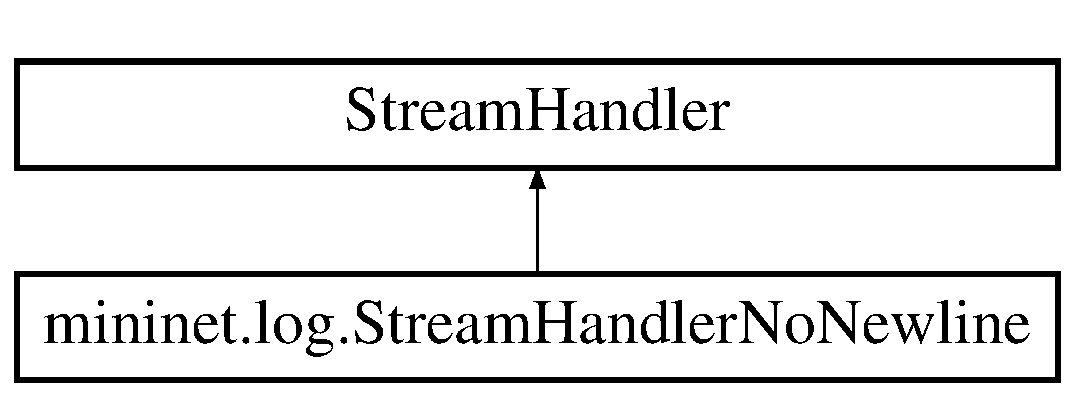
\includegraphics[height=2.000000cm]{classmininet_1_1log_1_1StreamHandlerNoNewline}
\end{center}
\end{figure}
\subsection*{Public Member Functions}
\begin{DoxyCompactItemize}
\item 
def \hyperlink{classmininet_1_1log_1_1StreamHandlerNoNewline_af7906c402ac800eae40d6f26e998894b}{emit}
\end{DoxyCompactItemize}


\subsection{Detailed Description}
\begin{DoxyVerb}StreamHandler that doesn't print newlines by default.
   Since StreamHandler automatically adds newlines, define a mod to more
   easily support interactive mode when we want it, or errors-only logging
   for running unit tests.\end{DoxyVerb}
 

\subsection{Member Function Documentation}
\hypertarget{classmininet_1_1log_1_1StreamHandlerNoNewline_af7906c402ac800eae40d6f26e998894b}{\index{mininet\-::log\-::\-Stream\-Handler\-No\-Newline@{mininet\-::log\-::\-Stream\-Handler\-No\-Newline}!emit@{emit}}
\index{emit@{emit}!mininet::log::StreamHandlerNoNewline@{mininet\-::log\-::\-Stream\-Handler\-No\-Newline}}
\subsubsection[{emit}]{\setlength{\rightskip}{0pt plus 5cm}def mininet.\-log.\-Stream\-Handler\-No\-Newline.\-emit (
\begin{DoxyParamCaption}
\item[{}]{self, }
\item[{}]{record}
\end{DoxyParamCaption}
)}}\label{classmininet_1_1log_1_1StreamHandlerNoNewline_af7906c402ac800eae40d6f26e998894b}
\begin{DoxyVerb}Emit a record.
   If a formatter is specified, it is used to format the record.
   The record is then written to the stream with a trailing newline
   [ N.B. this may be removed depending on feedback ]. If exception
   information is present, it is formatted using
   traceback.printException and appended to the stream.\end{DoxyVerb}
 

The documentation for this class was generated from the following file\-:\begin{DoxyCompactItemize}
\item 
log.\-py\end{DoxyCompactItemize}

\hypertarget{classmininet_1_1node_1_1Switch}{\section{mininet.\-node.\-Switch Class Reference}
\label{classmininet_1_1node_1_1Switch}\index{mininet.\-node.\-Switch@{mininet.\-node.\-Switch}}
}
Inheritance diagram for mininet.\-node.\-Switch\-:\begin{figure}[H]
\begin{center}
\leavevmode
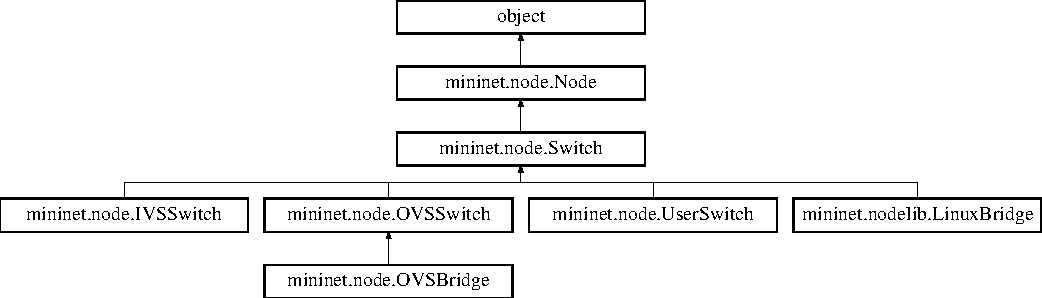
\includegraphics[height=4.000000cm]{classmininet_1_1node_1_1Switch}
\end{center}
\end{figure}
\subsection*{Public Member Functions}
\begin{DoxyCompactItemize}
\item 
def \hyperlink{classmininet_1_1node_1_1Switch_ad4abb0f4cb72e776d54c8327e262ef81}{\-\_\-\-\_\-init\-\_\-\-\_\-}
\item 
\hypertarget{classmininet_1_1node_1_1Switch_accc4b88c09e91e7ce7a7ec5fa8a5f22e}{def {\bfseries default\-Dpid}}\label{classmininet_1_1node_1_1Switch_accc4b88c09e91e7ce7a7ec5fa8a5f22e}

\item 
\hypertarget{classmininet_1_1node_1_1Switch_aae622083424ca6cacd7dd478dd7f86b0}{def {\bfseries default\-Intf}}\label{classmininet_1_1node_1_1Switch_aae622083424ca6cacd7dd478dd7f86b0}

\item 
def \hyperlink{classmininet_1_1node_1_1Switch_abce85860d0521c75d06fd237eec3fc4d}{send\-Cmd}
\item 
\hypertarget{classmininet_1_1node_1_1Switch_a4c888cb445b0e89ad07a5d7fbd8c1f1a}{def {\bfseries connected}}\label{classmininet_1_1node_1_1Switch_a4c888cb445b0e89ad07a5d7fbd8c1f1a}

\item 
def \hyperlink{classmininet_1_1node_1_1Switch_ac02447bd7e69ed56b09ca9a440a32459}{stop}
\item 
\hypertarget{classmininet_1_1node_1_1Switch_a95ab9bfcd138235fa4697a3782ad0c48}{def {\bfseries \-\_\-\-\_\-repr\-\_\-\-\_\-}}\label{classmininet_1_1node_1_1Switch_a95ab9bfcd138235fa4697a3782ad0c48}

\end{DoxyCompactItemize}
\subsection*{Public Attributes}
\begin{DoxyCompactItemize}
\item 
\hypertarget{classmininet_1_1node_1_1Switch_a7d9ecaa2ae7a2a1894bd3d936d8fbbdc}{{\bfseries dpid}}\label{classmininet_1_1node_1_1Switch_a7d9ecaa2ae7a2a1894bd3d936d8fbbdc}

\item 
\hypertarget{classmininet_1_1node_1_1Switch_a9a98d55c899be0d4ca8bfb7cd2e53beb}{{\bfseries opts}}\label{classmininet_1_1node_1_1Switch_a9a98d55c899be0d4ca8bfb7cd2e53beb}

\item 
\hypertarget{classmininet_1_1node_1_1Switch_a73a2d105dc1887e10901bcdbc2fa186c}{{\bfseries listen\-Port}}\label{classmininet_1_1node_1_1Switch_a73a2d105dc1887e10901bcdbc2fa186c}

\item 
\hypertarget{classmininet_1_1node_1_1Switch_a783620ed7dc731301a91dc9f58698bbe}{{\bfseries control\-Intf}}\label{classmininet_1_1node_1_1Switch_a783620ed7dc731301a91dc9f58698bbe}

\end{DoxyCompactItemize}
\subsection*{Static Public Attributes}
\begin{DoxyCompactItemize}
\item 
\hypertarget{classmininet_1_1node_1_1Switch_a56ab4dc0fa30ebfe9df532d6e42e09a9}{int {\bfseries port\-Base} = 1}\label{classmininet_1_1node_1_1Switch_a56ab4dc0fa30ebfe9df532d6e42e09a9}

\item 
\hypertarget{classmininet_1_1node_1_1Switch_a0fbabf15d17e87acac0bdde26f69ea6c}{int {\bfseries dpid\-Len} = 16}\label{classmininet_1_1node_1_1Switch_a0fbabf15d17e87acac0bdde26f69ea6c}

\end{DoxyCompactItemize}


\subsection{Detailed Description}
\begin{DoxyVerb}A Switch is a Node that is running (or has execed?)
   an OpenFlow switch.\end{DoxyVerb}
 

\subsection{Constructor \& Destructor Documentation}
\hypertarget{classmininet_1_1node_1_1Switch_ad4abb0f4cb72e776d54c8327e262ef81}{\index{mininet\-::node\-::\-Switch@{mininet\-::node\-::\-Switch}!\-\_\-\-\_\-init\-\_\-\-\_\-@{\-\_\-\-\_\-init\-\_\-\-\_\-}}
\index{\-\_\-\-\_\-init\-\_\-\-\_\-@{\-\_\-\-\_\-init\-\_\-\-\_\-}!mininet::node::Switch@{mininet\-::node\-::\-Switch}}
\subsubsection[{\-\_\-\-\_\-init\-\_\-\-\_\-}]{\setlength{\rightskip}{0pt plus 5cm}def mininet.\-node.\-Switch.\-\_\-\-\_\-init\-\_\-\-\_\- (
\begin{DoxyParamCaption}
\item[{}]{self, }
\item[{}]{name, }
\item[{}]{dpid = {\ttfamily None}, }
\item[{}]{opts = {\ttfamily ''}, }
\item[{}]{listen\-Port = {\ttfamily None}, }
\item[{}]{params}
\end{DoxyParamCaption}
)}}\label{classmininet_1_1node_1_1Switch_ad4abb0f4cb72e776d54c8327e262ef81}
\begin{DoxyVerb}dpid: dpid hex string (or None to derive from name, e.g. s1 -> 1)
   opts: additional switch options
   listenPort: port to listen on for dpctl connections\end{DoxyVerb}
 

\subsection{Member Function Documentation}
\hypertarget{classmininet_1_1node_1_1Switch_abce85860d0521c75d06fd237eec3fc4d}{\index{mininet\-::node\-::\-Switch@{mininet\-::node\-::\-Switch}!send\-Cmd@{send\-Cmd}}
\index{send\-Cmd@{send\-Cmd}!mininet::node::Switch@{mininet\-::node\-::\-Switch}}
\subsubsection[{send\-Cmd}]{\setlength{\rightskip}{0pt plus 5cm}def mininet.\-node.\-Switch.\-send\-Cmd (
\begin{DoxyParamCaption}
\item[{}]{self, }
\item[{}]{cmd, }
\item[{}]{kwargs}
\end{DoxyParamCaption}
)}}\label{classmininet_1_1node_1_1Switch_abce85860d0521c75d06fd237eec3fc4d}
\begin{DoxyVerb}Send command to Node.
   cmd: string\end{DoxyVerb}
 \hypertarget{classmininet_1_1node_1_1Switch_ac02447bd7e69ed56b09ca9a440a32459}{\index{mininet\-::node\-::\-Switch@{mininet\-::node\-::\-Switch}!stop@{stop}}
\index{stop@{stop}!mininet::node::Switch@{mininet\-::node\-::\-Switch}}
\subsubsection[{stop}]{\setlength{\rightskip}{0pt plus 5cm}def mininet.\-node.\-Switch.\-stop (
\begin{DoxyParamCaption}
\item[{}]{self, }
\item[{}]{delete\-Intfs = {\ttfamily True}}
\end{DoxyParamCaption}
)}}\label{classmininet_1_1node_1_1Switch_ac02447bd7e69ed56b09ca9a440a32459}
\begin{DoxyVerb}Stop switch
   deleteIntfs: delete interfaces? (True)\end{DoxyVerb}
 

The documentation for this class was generated from the following file\-:\begin{DoxyCompactItemize}
\item 
node.\-py\end{DoxyCompactItemize}

\hypertarget{classmininet_1_1link_1_1TCIntf}{\section{mininet.\-link.\-T\-C\-Intf Class Reference}
\label{classmininet_1_1link_1_1TCIntf}\index{mininet.\-link.\-T\-C\-Intf@{mininet.\-link.\-T\-C\-Intf}}
}
Inheritance diagram for mininet.\-link.\-T\-C\-Intf\-:\begin{figure}[H]
\begin{center}
\leavevmode
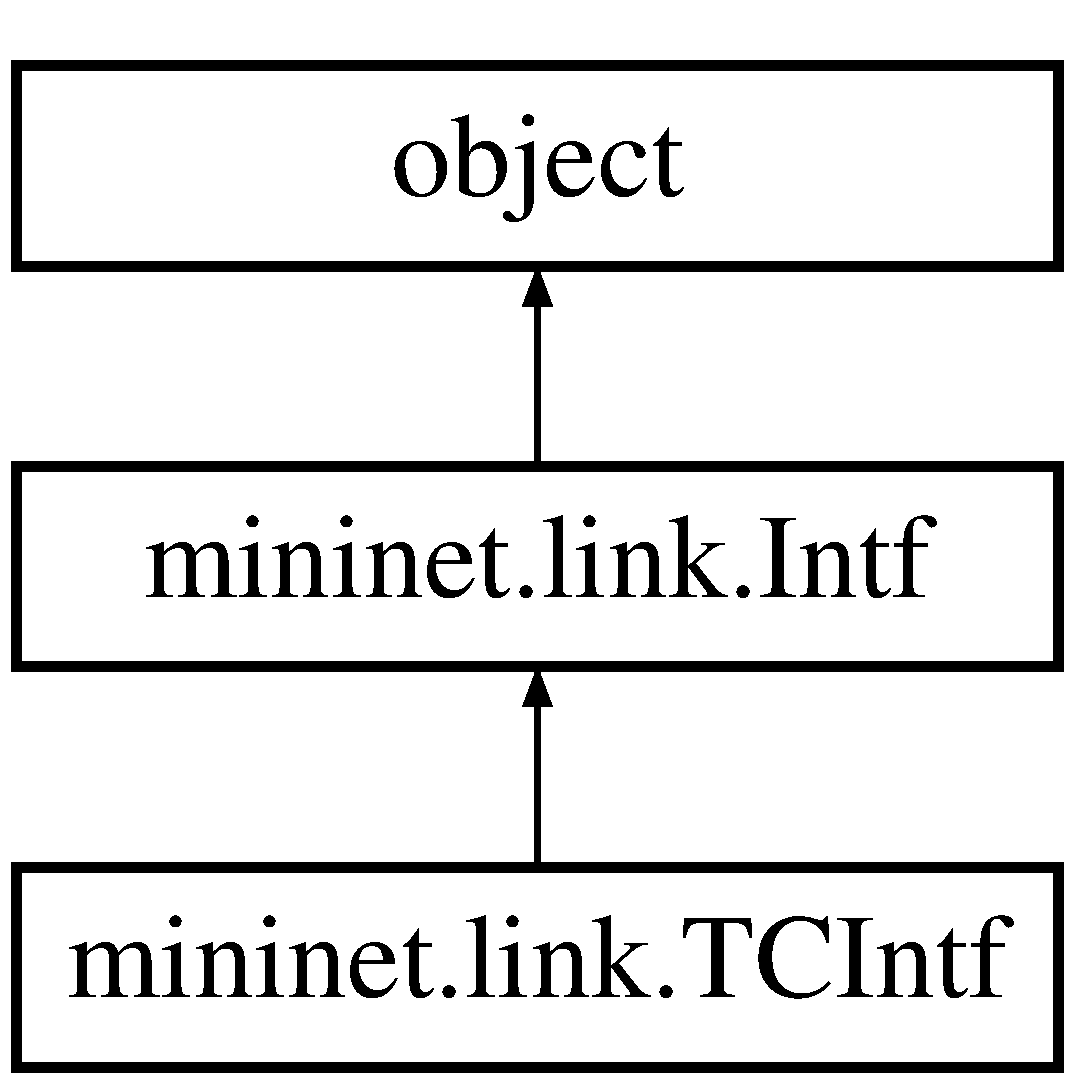
\includegraphics[height=3.000000cm]{classmininet_1_1link_1_1TCIntf}
\end{center}
\end{figure}
\subsection*{Public Member Functions}
\begin{DoxyCompactItemize}
\item 
\hypertarget{classmininet_1_1link_1_1TCIntf_a7e422dc20c9a702d693e9899f709e326}{def {\bfseries bw\-Cmds}}\label{classmininet_1_1link_1_1TCIntf_a7e422dc20c9a702d693e9899f709e326}

\item 
\hypertarget{classmininet_1_1link_1_1TCIntf_ac4371d8bff5144a4f66765084957afe6}{def {\bfseries tc}}\label{classmininet_1_1link_1_1TCIntf_ac4371d8bff5144a4f66765084957afe6}

\item 
\hypertarget{classmininet_1_1link_1_1TCIntf_a4e9cf4cb9e39771a537fa4ec717bd0a4}{def {\bfseries config}}\label{classmininet_1_1link_1_1TCIntf_a4e9cf4cb9e39771a537fa4ec717bd0a4}

\end{DoxyCompactItemize}
\subsection*{Static Public Member Functions}
\begin{DoxyCompactItemize}
\item 
\hypertarget{classmininet_1_1link_1_1TCIntf_aa75efea716cfdf857742e5a4bc5f94ae}{def {\bfseries delay\-Cmds}}\label{classmininet_1_1link_1_1TCIntf_aa75efea716cfdf857742e5a4bc5f94ae}

\end{DoxyCompactItemize}
\subsection*{Static Public Attributes}
\begin{DoxyCompactItemize}
\item 
\hypertarget{classmininet_1_1link_1_1TCIntf_aefe3cc2d66662f5aeef18a55f1796146}{int {\bfseries bw\-Param\-Max} = 1000}\label{classmininet_1_1link_1_1TCIntf_aefe3cc2d66662f5aeef18a55f1796146}

\end{DoxyCompactItemize}
\subsection*{Additional Inherited Members}


\subsection{Detailed Description}
\begin{DoxyVerb}Interface customized by tc (traffic control) utility
   Allows specification of bandwidth limits (various methods)
   as well as delay, loss and max queue length\end{DoxyVerb}
 

The documentation for this class was generated from the following file\-:\begin{DoxyCompactItemize}
\item 
link.\-py\end{DoxyCompactItemize}

\hypertarget{classmininet_1_1link_1_1TCLink}{\section{mininet.\-link.\-T\-C\-Link Class Reference}
\label{classmininet_1_1link_1_1TCLink}\index{mininet.\-link.\-T\-C\-Link@{mininet.\-link.\-T\-C\-Link}}
}
Inheritance diagram for mininet.\-link.\-T\-C\-Link\-:\begin{figure}[H]
\begin{center}
\leavevmode
\includegraphics[height=3.000000cm]{classmininet_1_1link_1_1TCLink}
\end{center}
\end{figure}
\subsection*{Public Member Functions}
\begin{DoxyCompactItemize}
\item 
\hypertarget{classmininet_1_1link_1_1TCLink_a443b8c7bf82abbe41eac677d788bfbc1}{def {\bfseries \-\_\-\-\_\-init\-\_\-\-\_\-}}\label{classmininet_1_1link_1_1TCLink_a443b8c7bf82abbe41eac677d788bfbc1}

\end{DoxyCompactItemize}
\subsection*{Additional Inherited Members}


The documentation for this class was generated from the following file\-:\begin{DoxyCompactItemize}
\item 
link.\-py\end{DoxyCompactItemize}

\hypertarget{classmininet_1_1topo_1_1Topo}{\section{mininet.\-topo.\-Topo Class Reference}
\label{classmininet_1_1topo_1_1Topo}\index{mininet.\-topo.\-Topo@{mininet.\-topo.\-Topo}}
}
Inheritance diagram for mininet.\-topo.\-Topo\-:\begin{figure}[H]
\begin{center}
\leavevmode
\includegraphics[height=1.828571cm]{classmininet_1_1topo_1_1Topo}
\end{center}
\end{figure}
\subsection*{Public Member Functions}
\begin{DoxyCompactItemize}
\item 
def \hyperlink{classmininet_1_1topo_1_1Topo_aa676f9d1a195133f173f73191aa3488b}{\-\_\-\-\_\-init\-\_\-\-\_\-}
\item 
\hypertarget{classmininet_1_1topo_1_1Topo_af49b0fef111262d6c0bd08e7977f9ffc}{def {\bfseries build}}\label{classmininet_1_1topo_1_1Topo_af49b0fef111262d6c0bd08e7977f9ffc}

\item 
def \hyperlink{classmininet_1_1topo_1_1Topo_ad49002a42e5525bbe9e0136d10d9b72d}{add\-Node}
\item 
def \hyperlink{classmininet_1_1topo_1_1Topo_a4649e48317e0b09f84ac5c6a88424194}{add\-Host}
\item 
def \hyperlink{classmininet_1_1topo_1_1Topo_acf5880d959db9ef7c3be45d1d6dfc72a}{add\-Station}
\item 
def \hyperlink{classmininet_1_1topo_1_1Topo_a8506ad67498aefb4a42ad1cd51576b38}{add\-Switch}
\item 
def \hyperlink{classmininet_1_1topo_1_1Topo_abf65ac2a53a0e0b0f27ac472723a1c37}{add\-Base\-Station}
\item 
def \hyperlink{classmininet_1_1topo_1_1Topo_ade9840eb4826cb17d5c6bc868e762fa3}{add\-Link}
\item 
\hypertarget{classmininet_1_1topo_1_1Topo_a4386138cc13f285c9c963367a492187d}{def {\bfseries nodes}}\label{classmininet_1_1topo_1_1Topo_a4386138cc13f285c9c963367a492187d}

\item 
\hypertarget{classmininet_1_1topo_1_1Topo_a47cc4a860b8806784fb84bb39f8212d8}{def {\bfseries is\-Switch}}\label{classmininet_1_1topo_1_1Topo_a47cc4a860b8806784fb84bb39f8212d8}

\item 
def \hyperlink{classmininet_1_1topo_1_1Topo_ac69689ade0c4416b7f1d726867e5034f}{switches}
\item 
def \hyperlink{classmininet_1_1topo_1_1Topo_a0f802790abc965ca8f775ae218e1dbb8}{base\-Stations}
\item 
def \hyperlink{classmininet_1_1topo_1_1Topo_a087a4818bbb5a1beba067fce4f009969}{hosts}
\item 
def \hyperlink{classmininet_1_1topo_1_1Topo_a900cec05bd380b32a60e0fc5371bcb29}{iter\-Links}
\item 
def \hyperlink{classmininet_1_1topo_1_1Topo_ad30a63eb5f3a910d331e33e34fe9adbb}{links}
\item 
def \hyperlink{classmininet_1_1topo_1_1Topo_ab83082737d1c8f4cba2da043a9ac91f9}{add\-Port}
\item 
def \hyperlink{classmininet_1_1topo_1_1Topo_af076ac0a3d9a21fbdb5703fc251c6fe8}{port}
\item 
\hypertarget{classmininet_1_1topo_1_1Topo_ae8e97604bcab29d2441e016311381aa6}{def {\bfseries link\-Info}}\label{classmininet_1_1topo_1_1Topo_ae8e97604bcab29d2441e016311381aa6}

\item 
\hypertarget{classmininet_1_1topo_1_1Topo_a0e4081c6546a423a8724a7ac61ef9525}{def {\bfseries setlink\-Info}}\label{classmininet_1_1topo_1_1Topo_a0e4081c6546a423a8724a7ac61ef9525}

\item 
\hypertarget{classmininet_1_1topo_1_1Topo_ae0a5d2f82528cea4bc6c9182e7be3a26}{def {\bfseries node\-Info}}\label{classmininet_1_1topo_1_1Topo_ae0a5d2f82528cea4bc6c9182e7be3a26}

\item 
\hypertarget{classmininet_1_1topo_1_1Topo_a50c251ee1ab591319040c11e437e151f}{def {\bfseries set\-Node\-Info}}\label{classmininet_1_1topo_1_1Topo_a50c251ee1ab591319040c11e437e151f}

\item 
def \hyperlink{classmininet_1_1topo_1_1Topo_aa26e0fa82e7ef2f76973bfbffa58111c}{convert\-To}
\end{DoxyCompactItemize}
\subsection*{Static Public Member Functions}
\begin{DoxyCompactItemize}
\item 
\hypertarget{classmininet_1_1topo_1_1Topo_a916097bac0c027b93e20ef7b2f3411bb}{def {\bfseries sorted}}\label{classmininet_1_1topo_1_1Topo_a916097bac0c027b93e20ef7b2f3411bb}

\end{DoxyCompactItemize}
\subsection*{Public Attributes}
\begin{DoxyCompactItemize}
\item 
\hypertarget{classmininet_1_1topo_1_1Topo_a70bbf3eeb5ca78c00bed747550f200fb}{{\bfseries g}}\label{classmininet_1_1topo_1_1Topo_a70bbf3eeb5ca78c00bed747550f200fb}

\item 
\hypertarget{classmininet_1_1topo_1_1Topo_a00bfbf1a906cee8ffedb1b580be4cc9e}{{\bfseries hopts}}\label{classmininet_1_1topo_1_1Topo_a00bfbf1a906cee8ffedb1b580be4cc9e}

\item 
\hypertarget{classmininet_1_1topo_1_1Topo_a024d34f258d27a1ea25fba80f51e2336}{{\bfseries sopts}}\label{classmininet_1_1topo_1_1Topo_a024d34f258d27a1ea25fba80f51e2336}

\item 
\hypertarget{classmininet_1_1topo_1_1Topo_afd3106f9f94f83c5b18cc7bd5c5881c8}{{\bfseries lopts}}\label{classmininet_1_1topo_1_1Topo_afd3106f9f94f83c5b18cc7bd5c5881c8}

\item 
\hypertarget{classmininet_1_1topo_1_1Topo_a5601b1d8b5d657cc7d47342d6c09787f}{{\bfseries ports}}\label{classmininet_1_1topo_1_1Topo_a5601b1d8b5d657cc7d47342d6c09787f}

\end{DoxyCompactItemize}


\subsection{Constructor \& Destructor Documentation}
\hypertarget{classmininet_1_1topo_1_1Topo_aa676f9d1a195133f173f73191aa3488b}{\index{mininet\-::topo\-::\-Topo@{mininet\-::topo\-::\-Topo}!\-\_\-\-\_\-init\-\_\-\-\_\-@{\-\_\-\-\_\-init\-\_\-\-\_\-}}
\index{\-\_\-\-\_\-init\-\_\-\-\_\-@{\-\_\-\-\_\-init\-\_\-\-\_\-}!mininet::topo::Topo@{mininet\-::topo\-::\-Topo}}
\subsubsection[{\-\_\-\-\_\-init\-\_\-\-\_\-}]{\setlength{\rightskip}{0pt plus 5cm}def mininet.\-topo.\-Topo.\-\_\-\-\_\-init\-\_\-\-\_\- (
\begin{DoxyParamCaption}
\item[{}]{self, }
\item[{}]{args, }
\item[{}]{params}
\end{DoxyParamCaption}
)}}\label{classmininet_1_1topo_1_1Topo_aa676f9d1a195133f173f73191aa3488b}
\begin{DoxyVerb}Topo object.
   Optional named parameters:
   hinfo: default host options
   sopts: default switch options
   lopts: default link options
   calls build()\end{DoxyVerb}
 

\subsection{Member Function Documentation}
\hypertarget{classmininet_1_1topo_1_1Topo_abf65ac2a53a0e0b0f27ac472723a1c37}{\index{mininet\-::topo\-::\-Topo@{mininet\-::topo\-::\-Topo}!add\-Base\-Station@{add\-Base\-Station}}
\index{add\-Base\-Station@{add\-Base\-Station}!mininet::topo::Topo@{mininet\-::topo\-::\-Topo}}
\subsubsection[{add\-Base\-Station}]{\setlength{\rightskip}{0pt plus 5cm}def mininet.\-topo.\-Topo.\-add\-Base\-Station (
\begin{DoxyParamCaption}
\item[{}]{self, }
\item[{}]{name, }
\item[{}]{opts}
\end{DoxyParamCaption}
)}}\label{classmininet_1_1topo_1_1Topo_abf65ac2a53a0e0b0f27ac472723a1c37}
\begin{DoxyVerb}Convenience method: Add switch to graph.
   name: switch name
   opts: switch options
   returns: switch name\end{DoxyVerb}
 \hypertarget{classmininet_1_1topo_1_1Topo_a4649e48317e0b09f84ac5c6a88424194}{\index{mininet\-::topo\-::\-Topo@{mininet\-::topo\-::\-Topo}!add\-Host@{add\-Host}}
\index{add\-Host@{add\-Host}!mininet::topo::Topo@{mininet\-::topo\-::\-Topo}}
\subsubsection[{add\-Host}]{\setlength{\rightskip}{0pt plus 5cm}def mininet.\-topo.\-Topo.\-add\-Host (
\begin{DoxyParamCaption}
\item[{}]{self, }
\item[{}]{name, }
\item[{}]{opts}
\end{DoxyParamCaption}
)}}\label{classmininet_1_1topo_1_1Topo_a4649e48317e0b09f84ac5c6a88424194}
\begin{DoxyVerb}Convenience method: Add host to graph.
   name: host name
   opts: host options
   returns: host name\end{DoxyVerb}
 \hypertarget{classmininet_1_1topo_1_1Topo_ade9840eb4826cb17d5c6bc868e762fa3}{\index{mininet\-::topo\-::\-Topo@{mininet\-::topo\-::\-Topo}!add\-Link@{add\-Link}}
\index{add\-Link@{add\-Link}!mininet::topo::Topo@{mininet\-::topo\-::\-Topo}}
\subsubsection[{add\-Link}]{\setlength{\rightskip}{0pt plus 5cm}def mininet.\-topo.\-Topo.\-add\-Link (
\begin{DoxyParamCaption}
\item[{}]{self, }
\item[{}]{node1, }
\item[{}]{node2, }
\item[{}]{port1 = {\ttfamily None}, }
\item[{}]{port2 = {\ttfamily None}, }
\item[{}]{key = {\ttfamily None}, }
\item[{}]{opts}
\end{DoxyParamCaption}
)}}\label{classmininet_1_1topo_1_1Topo_ade9840eb4826cb17d5c6bc868e762fa3}
\begin{DoxyVerb}node1, node2: nodes to link together
   port1, port2: ports (optional)
   opts: link options (optional)
   returns: link info key\end{DoxyVerb}
 \hypertarget{classmininet_1_1topo_1_1Topo_ad49002a42e5525bbe9e0136d10d9b72d}{\index{mininet\-::topo\-::\-Topo@{mininet\-::topo\-::\-Topo}!add\-Node@{add\-Node}}
\index{add\-Node@{add\-Node}!mininet::topo::Topo@{mininet\-::topo\-::\-Topo}}
\subsubsection[{add\-Node}]{\setlength{\rightskip}{0pt plus 5cm}def mininet.\-topo.\-Topo.\-add\-Node (
\begin{DoxyParamCaption}
\item[{}]{self, }
\item[{}]{name, }
\item[{}]{opts}
\end{DoxyParamCaption}
)}}\label{classmininet_1_1topo_1_1Topo_ad49002a42e5525bbe9e0136d10d9b72d}
\begin{DoxyVerb}Add Node to graph.
   name: name
   opts: node options
   returns: node name\end{DoxyVerb}
 \hypertarget{classmininet_1_1topo_1_1Topo_ab83082737d1c8f4cba2da043a9ac91f9}{\index{mininet\-::topo\-::\-Topo@{mininet\-::topo\-::\-Topo}!add\-Port@{add\-Port}}
\index{add\-Port@{add\-Port}!mininet::topo::Topo@{mininet\-::topo\-::\-Topo}}
\subsubsection[{add\-Port}]{\setlength{\rightskip}{0pt plus 5cm}def mininet.\-topo.\-Topo.\-add\-Port (
\begin{DoxyParamCaption}
\item[{}]{self, }
\item[{}]{src, }
\item[{}]{dst, }
\item[{}]{sport = {\ttfamily None}, }
\item[{}]{dport = {\ttfamily None}}
\end{DoxyParamCaption}
)}}\label{classmininet_1_1topo_1_1Topo_ab83082737d1c8f4cba2da043a9ac91f9}
\begin{DoxyVerb}Generate port mapping for new edge.
    src: source switch name
    dst: destination switch name\end{DoxyVerb}
 \hypertarget{classmininet_1_1topo_1_1Topo_acf5880d959db9ef7c3be45d1d6dfc72a}{\index{mininet\-::topo\-::\-Topo@{mininet\-::topo\-::\-Topo}!add\-Station@{add\-Station}}
\index{add\-Station@{add\-Station}!mininet::topo::Topo@{mininet\-::topo\-::\-Topo}}
\subsubsection[{add\-Station}]{\setlength{\rightskip}{0pt plus 5cm}def mininet.\-topo.\-Topo.\-add\-Station (
\begin{DoxyParamCaption}
\item[{}]{self, }
\item[{}]{name, }
\item[{}]{opts}
\end{DoxyParamCaption}
)}}\label{classmininet_1_1topo_1_1Topo_acf5880d959db9ef7c3be45d1d6dfc72a}
\begin{DoxyVerb}Convenience method: Add host to graph.
   name: host name
   opts: host options
   returns: host name\end{DoxyVerb}
 \hypertarget{classmininet_1_1topo_1_1Topo_a8506ad67498aefb4a42ad1cd51576b38}{\index{mininet\-::topo\-::\-Topo@{mininet\-::topo\-::\-Topo}!add\-Switch@{add\-Switch}}
\index{add\-Switch@{add\-Switch}!mininet::topo::Topo@{mininet\-::topo\-::\-Topo}}
\subsubsection[{add\-Switch}]{\setlength{\rightskip}{0pt plus 5cm}def mininet.\-topo.\-Topo.\-add\-Switch (
\begin{DoxyParamCaption}
\item[{}]{self, }
\item[{}]{name, }
\item[{}]{opts}
\end{DoxyParamCaption}
)}}\label{classmininet_1_1topo_1_1Topo_a8506ad67498aefb4a42ad1cd51576b38}
\begin{DoxyVerb}Convenience method: Add switch to graph.
   name: switch name
   opts: switch options
   returns: switch name\end{DoxyVerb}
 \hypertarget{classmininet_1_1topo_1_1Topo_a0f802790abc965ca8f775ae218e1dbb8}{\index{mininet\-::topo\-::\-Topo@{mininet\-::topo\-::\-Topo}!base\-Stations@{base\-Stations}}
\index{base\-Stations@{base\-Stations}!mininet::topo::Topo@{mininet\-::topo\-::\-Topo}}
\subsubsection[{base\-Stations}]{\setlength{\rightskip}{0pt plus 5cm}def mininet.\-topo.\-Topo.\-base\-Stations (
\begin{DoxyParamCaption}
\item[{}]{self, }
\item[{}]{sort = {\ttfamily True}}
\end{DoxyParamCaption}
)}}\label{classmininet_1_1topo_1_1Topo_a0f802790abc965ca8f775ae218e1dbb8}
\begin{DoxyVerb}Return BaseStations.
   sort: sort basestations alphabetically
   returns: dpids list of dpids\end{DoxyVerb}
 \hypertarget{classmininet_1_1topo_1_1Topo_aa26e0fa82e7ef2f76973bfbffa58111c}{\index{mininet\-::topo\-::\-Topo@{mininet\-::topo\-::\-Topo}!convert\-To@{convert\-To}}
\index{convert\-To@{convert\-To}!mininet::topo::Topo@{mininet\-::topo\-::\-Topo}}
\subsubsection[{convert\-To}]{\setlength{\rightskip}{0pt plus 5cm}def mininet.\-topo.\-Topo.\-convert\-To (
\begin{DoxyParamCaption}
\item[{}]{self, }
\item[{}]{cls, }
\item[{}]{data = {\ttfamily True}, }
\item[{}]{keys = {\ttfamily True}}
\end{DoxyParamCaption}
)}}\label{classmininet_1_1topo_1_1Topo_aa26e0fa82e7ef2f76973bfbffa58111c}
\begin{DoxyVerb}Convert to a new object of networkx.MultiGraph-like class cls
   data: include node and edge data (default True)
   keys: include edge keys as well as edge data (default True)\end{DoxyVerb}
 \hypertarget{classmininet_1_1topo_1_1Topo_a087a4818bbb5a1beba067fce4f009969}{\index{mininet\-::topo\-::\-Topo@{mininet\-::topo\-::\-Topo}!hosts@{hosts}}
\index{hosts@{hosts}!mininet::topo::Topo@{mininet\-::topo\-::\-Topo}}
\subsubsection[{hosts}]{\setlength{\rightskip}{0pt plus 5cm}def mininet.\-topo.\-Topo.\-hosts (
\begin{DoxyParamCaption}
\item[{}]{self, }
\item[{}]{sort = {\ttfamily True}}
\end{DoxyParamCaption}
)}}\label{classmininet_1_1topo_1_1Topo_a087a4818bbb5a1beba067fce4f009969}
\begin{DoxyVerb}Return hosts.
   sort: sort hosts alphabetically
   returns: list of hosts\end{DoxyVerb}
 \hypertarget{classmininet_1_1topo_1_1Topo_a900cec05bd380b32a60e0fc5371bcb29}{\index{mininet\-::topo\-::\-Topo@{mininet\-::topo\-::\-Topo}!iter\-Links@{iter\-Links}}
\index{iter\-Links@{iter\-Links}!mininet::topo::Topo@{mininet\-::topo\-::\-Topo}}
\subsubsection[{iter\-Links}]{\setlength{\rightskip}{0pt plus 5cm}def mininet.\-topo.\-Topo.\-iter\-Links (
\begin{DoxyParamCaption}
\item[{}]{self, }
\item[{}]{with\-Keys = {\ttfamily False}, }
\item[{}]{with\-Info = {\ttfamily False}}
\end{DoxyParamCaption}
)}}\label{classmininet_1_1topo_1_1Topo_a900cec05bd380b32a60e0fc5371bcb29}
\begin{DoxyVerb}Return links (iterator)
   withKeys: return link keys
   withInfo: return link info
   returns: list of ( src, dst [,key, info ] )\end{DoxyVerb}
 \hypertarget{classmininet_1_1topo_1_1Topo_ad30a63eb5f3a910d331e33e34fe9adbb}{\index{mininet\-::topo\-::\-Topo@{mininet\-::topo\-::\-Topo}!links@{links}}
\index{links@{links}!mininet::topo::Topo@{mininet\-::topo\-::\-Topo}}
\subsubsection[{links}]{\setlength{\rightskip}{0pt plus 5cm}def mininet.\-topo.\-Topo.\-links (
\begin{DoxyParamCaption}
\item[{}]{self, }
\item[{}]{sort = {\ttfamily False}, }
\item[{}]{with\-Keys = {\ttfamily False}, }
\item[{}]{with\-Info = {\ttfamily False}}
\end{DoxyParamCaption}
)}}\label{classmininet_1_1topo_1_1Topo_ad30a63eb5f3a910d331e33e34fe9adbb}
\begin{DoxyVerb}Return links
   sort: sort links alphabetically, preserving (src, dst) order
   withKeys: return link keys
   withInfo: return link info
   returns: list of ( src, dst [,key, info ] )\end{DoxyVerb}
 \hypertarget{classmininet_1_1topo_1_1Topo_af076ac0a3d9a21fbdb5703fc251c6fe8}{\index{mininet\-::topo\-::\-Topo@{mininet\-::topo\-::\-Topo}!port@{port}}
\index{port@{port}!mininet::topo::Topo@{mininet\-::topo\-::\-Topo}}
\subsubsection[{port}]{\setlength{\rightskip}{0pt plus 5cm}def mininet.\-topo.\-Topo.\-port (
\begin{DoxyParamCaption}
\item[{}]{self, }
\item[{}]{src, }
\item[{}]{dst}
\end{DoxyParamCaption}
)}}\label{classmininet_1_1topo_1_1Topo_af076ac0a3d9a21fbdb5703fc251c6fe8}
\begin{DoxyVerb}Get port numbers.
    src: source switch name
    dst: destination switch name
    sport: optional source port (otherwise use lowest src port)
    returns: tuple (sport, dport), where
sport = port on source switch leading to the destination switch
dport = port on destination switch leading to the source switch
    Note that you can also look up ports using linkInfo()\end{DoxyVerb}
 \hypertarget{classmininet_1_1topo_1_1Topo_ac69689ade0c4416b7f1d726867e5034f}{\index{mininet\-::topo\-::\-Topo@{mininet\-::topo\-::\-Topo}!switches@{switches}}
\index{switches@{switches}!mininet::topo::Topo@{mininet\-::topo\-::\-Topo}}
\subsubsection[{switches}]{\setlength{\rightskip}{0pt plus 5cm}def mininet.\-topo.\-Topo.\-switches (
\begin{DoxyParamCaption}
\item[{}]{self, }
\item[{}]{sort = {\ttfamily True}}
\end{DoxyParamCaption}
)}}\label{classmininet_1_1topo_1_1Topo_ac69689ade0c4416b7f1d726867e5034f}
\begin{DoxyVerb}Return switches.
   sort: sort switches alphabetically
   returns: dpids list of dpids\end{DoxyVerb}
 

The documentation for this class was generated from the following file\-:\begin{DoxyCompactItemize}
\item 
topo.\-py\end{DoxyCompactItemize}

\hypertarget{classmininet_1_1topolib_1_1TorusTopo}{\section{mininet.\-topolib.\-Torus\-Topo Class Reference}
\label{classmininet_1_1topolib_1_1TorusTopo}\index{mininet.\-topolib.\-Torus\-Topo@{mininet.\-topolib.\-Torus\-Topo}}
}
Inheritance diagram for mininet.\-topolib.\-Torus\-Topo\-:\begin{figure}[H]
\begin{center}
\leavevmode
\includegraphics[height=3.000000cm]{classmininet_1_1topolib_1_1TorusTopo}
\end{center}
\end{figure}
\subsection*{Public Member Functions}
\begin{DoxyCompactItemize}
\item 
\hypertarget{classmininet_1_1topolib_1_1TorusTopo_a7cd10b420d90c4892d6de451254d795b}{def {\bfseries build}}\label{classmininet_1_1topolib_1_1TorusTopo_a7cd10b420d90c4892d6de451254d795b}

\end{DoxyCompactItemize}
\subsection*{Additional Inherited Members}


\subsection{Detailed Description}
\begin{DoxyVerb}2-D Torus topology
   WARNING: this topology has LOOPS and WILL NOT WORK
   with the default controller or any Ethernet bridge
   without STP turned on! It can be used with STP, e.g.:
   # mn --topo torus,3,3 --switch lxbr,stp=1 --test pingall\end{DoxyVerb}
 

The documentation for this class was generated from the following file\-:\begin{DoxyCompactItemize}
\item 
topolib.\-py\end{DoxyCompactItemize}

\hypertarget{classmininet_1_1topolib_1_1TreeTopo}{\section{mininet.\-topolib.\-Tree\-Topo Class Reference}
\label{classmininet_1_1topolib_1_1TreeTopo}\index{mininet.\-topolib.\-Tree\-Topo@{mininet.\-topolib.\-Tree\-Topo}}
}
Inheritance diagram for mininet.\-topolib.\-Tree\-Topo\-:\begin{figure}[H]
\begin{center}
\leavevmode
\includegraphics[height=3.000000cm]{classmininet_1_1topolib_1_1TreeTopo}
\end{center}
\end{figure}
\subsection*{Public Member Functions}
\begin{DoxyCompactItemize}
\item 
\hypertarget{classmininet_1_1topolib_1_1TreeTopo_ae224f88e5afb1edc38f78a896b877ae1}{def {\bfseries build}}\label{classmininet_1_1topolib_1_1TreeTopo_ae224f88e5afb1edc38f78a896b877ae1}

\item 
def \hyperlink{classmininet_1_1topolib_1_1TreeTopo_aefae3c81588ee4c60168e1e8918abcd9}{add\-Tree}
\end{DoxyCompactItemize}
\subsection*{Public Attributes}
\begin{DoxyCompactItemize}
\item 
\hypertarget{classmininet_1_1topolib_1_1TreeTopo_abf208411938f3fc286234eed0889c833}{{\bfseries host\-Num}}\label{classmininet_1_1topolib_1_1TreeTopo_abf208411938f3fc286234eed0889c833}

\item 
\hypertarget{classmininet_1_1topolib_1_1TreeTopo_a41b1eefd3cc623350ec11971c9031ad0}{{\bfseries switch\-Num}}\label{classmininet_1_1topolib_1_1TreeTopo_a41b1eefd3cc623350ec11971c9031ad0}

\end{DoxyCompactItemize}
\subsection*{Additional Inherited Members}


\subsection{Member Function Documentation}
\hypertarget{classmininet_1_1topolib_1_1TreeTopo_aefae3c81588ee4c60168e1e8918abcd9}{\index{mininet\-::topolib\-::\-Tree\-Topo@{mininet\-::topolib\-::\-Tree\-Topo}!add\-Tree@{add\-Tree}}
\index{add\-Tree@{add\-Tree}!mininet::topolib::TreeTopo@{mininet\-::topolib\-::\-Tree\-Topo}}
\subsubsection[{add\-Tree}]{\setlength{\rightskip}{0pt plus 5cm}def mininet.\-topolib.\-Tree\-Topo.\-add\-Tree (
\begin{DoxyParamCaption}
\item[{}]{self, }
\item[{}]{depth, }
\item[{}]{fanout, }
\item[{}]{is\-Wi\-Fi}
\end{DoxyParamCaption}
)}}\label{classmininet_1_1topolib_1_1TreeTopo_aefae3c81588ee4c60168e1e8918abcd9}
\begin{DoxyVerb}Add a subtree starting with node n.
   returns: last node added\end{DoxyVerb}
 

The documentation for this class was generated from the following file\-:\begin{DoxyCompactItemize}
\item 
topolib.\-py\end{DoxyCompactItemize}

\hypertarget{classmininet_1_1wifiMobilityModels_1_1TruncatedLevyWalk}{\section{mininet.\-wifi\-Mobility\-Models.\-Truncated\-Levy\-Walk Class Reference}
\label{classmininet_1_1wifiMobilityModels_1_1TruncatedLevyWalk}\index{mininet.\-wifi\-Mobility\-Models.\-Truncated\-Levy\-Walk@{mininet.\-wifi\-Mobility\-Models.\-Truncated\-Levy\-Walk}}
}
Inheritance diagram for mininet.\-wifi\-Mobility\-Models.\-Truncated\-Levy\-Walk\-:\begin{figure}[H]
\begin{center}
\leavevmode
\includegraphics[height=3.000000cm]{classmininet_1_1wifiMobilityModels_1_1TruncatedLevyWalk}
\end{center}
\end{figure}
\subsection*{Public Member Functions}
\begin{DoxyCompactItemize}
\item 
def \hyperlink{classmininet_1_1wifiMobilityModels_1_1TruncatedLevyWalk_a63ef49f949e6ececbb962810d272cbf1}{\-\_\-\-\_\-init\-\_\-\-\_\-}
\end{DoxyCompactItemize}
\subsection*{Additional Inherited Members}


\subsection{Constructor \& Destructor Documentation}
\hypertarget{classmininet_1_1wifiMobilityModels_1_1TruncatedLevyWalk_a63ef49f949e6ececbb962810d272cbf1}{\index{mininet\-::wifi\-Mobility\-Models\-::\-Truncated\-Levy\-Walk@{mininet\-::wifi\-Mobility\-Models\-::\-Truncated\-Levy\-Walk}!\-\_\-\-\_\-init\-\_\-\-\_\-@{\-\_\-\-\_\-init\-\_\-\-\_\-}}
\index{\-\_\-\-\_\-init\-\_\-\-\_\-@{\-\_\-\-\_\-init\-\_\-\-\_\-}!mininet::wifiMobilityModels::TruncatedLevyWalk@{mininet\-::wifi\-Mobility\-Models\-::\-Truncated\-Levy\-Walk}}
\subsubsection[{\-\_\-\-\_\-init\-\_\-\-\_\-}]{\setlength{\rightskip}{0pt plus 5cm}def mininet.\-wifi\-Mobility\-Models.\-Truncated\-Levy\-Walk.\-\_\-\-\_\-init\-\_\-\-\_\- (
\begin{DoxyParamCaption}
\item[{}]{self, }
\item[{}]{nr\-\_\-nodes, }
\item[{}]{dimensions, }
\item[{}]{F\-L\-\_\-\-E\-X\-P = {\ttfamily -\/2.6}, }
\item[{}]{F\-L\-\_\-\-M\-A\-X = {\ttfamily 50.}, }
\item[{}]{W\-T\-\_\-\-E\-X\-P = {\ttfamily -\/1.8}, }
\item[{}]{W\-T\-\_\-\-M\-A\-X = {\ttfamily 100.}, }
\item[{}]{border\-\_\-policy = {\ttfamily 'reflect'}}
\end{DoxyParamCaption}
)}}\label{classmininet_1_1wifiMobilityModels_1_1TruncatedLevyWalk_a63ef49f949e6ececbb962810d272cbf1}
\begin{DoxyVerb}Truncated Levy Walk mobility model, based on the following paper:
Injong Rhee, Minsu Shin, Seongik Hong, Kyunghan Lee, and Song Chong. On the Levy-Walk Nature of Human Mobility. 
    In 2008 IEEE INFOCOM - Proceedings of the 27th Conference on Computer Communications, pages 924-932. April 2008.

The implementation is a special case of the more generic Stochastic Walk, 
in which both the flight length and waiting time distributions are truncated power laws,
with exponents set to FL_EXP and WT_EXP and truncated at FL_MAX and WT_MAX.
The node velocity is a function of the flight length.

Required arguments:

  *nr_nodes*:
    Integer, the number of nodes.
  
  *dimensions*:
    Tuple of Integers, the x and y dimensions of the simulation area.
  
keyword arguments:

  *FL_EXP*:
    Double, the exponent of the flight length distribution. Default is -2.6
    
  *FL_MAX*:
    Double, the maximum value of the flight length distribution. Default is 50
  
  *WT_EXP*:
    Double, the exponent of the waiting time distribution. Default is -1.8
    
  *WT_MAX*:
    Double, the maximum value of the waiting time distribution. Default is 100
    
  *border_policy*:
    String, either 'reflect' or 'wrap'. The policy that is used when the node arrives to the border.
    If 'reflect', the node reflects off the border.
    If 'wrap', the node reappears at the opposite edge (as in a torus-shaped area).
\end{DoxyVerb}
 

The documentation for this class was generated from the following file\-:\begin{DoxyCompactItemize}
\item 
wifi\-Mobility\-Models.\-py\end{DoxyCompactItemize}

\hypertarget{classmininet_1_1node_1_1UserSwitch}{\section{mininet.\-node.\-User\-Switch Class Reference}
\label{classmininet_1_1node_1_1UserSwitch}\index{mininet.\-node.\-User\-Switch@{mininet.\-node.\-User\-Switch}}
}
Inheritance diagram for mininet.\-node.\-User\-Switch\-:\begin{figure}[H]
\begin{center}
\leavevmode
\includegraphics[height=4.000000cm]{classmininet_1_1node_1_1UserSwitch}
\end{center}
\end{figure}
\subsection*{Public Member Functions}
\begin{DoxyCompactItemize}
\item 
def \hyperlink{classmininet_1_1node_1_1UserSwitch_ac22742d054d03bfa9b62ce4acd305b51}{\-\_\-\-\_\-init\-\_\-\-\_\-}
\item 
\hypertarget{classmininet_1_1node_1_1UserSwitch_a3cbcdd424e0ddb14ff7705f6e470e883}{def {\bfseries setup}}\label{classmininet_1_1node_1_1UserSwitch_a3cbcdd424e0ddb14ff7705f6e470e883}

\item 
\hypertarget{classmininet_1_1node_1_1UserSwitch_ad33189e5046bd69654a229340a4dacca}{def {\bfseries dpctl}}\label{classmininet_1_1node_1_1UserSwitch_ad33189e5046bd69654a229340a4dacca}

\item 
\hypertarget{classmininet_1_1node_1_1UserSwitch_a06ee71c1851b5a6ec63012be4bb64606}{def {\bfseries connected}}\label{classmininet_1_1node_1_1UserSwitch_a06ee71c1851b5a6ec63012be4bb64606}

\item 
def \hyperlink{classmininet_1_1node_1_1UserSwitch_af5651c986ae4c50c04a12138da52b854}{start}
\item 
def \hyperlink{classmininet_1_1node_1_1UserSwitch_a5e07816289fa23921ab679b3eb019b6b}{stop}
\end{DoxyCompactItemize}
\subsection*{Static Public Member Functions}
\begin{DoxyCompactItemize}
\item 
def \hyperlink{classmininet_1_1node_1_1UserSwitch_aa1ff2eb96e96a859fc2824445d7f4a8e}{T\-C\-Reapply}
\end{DoxyCompactItemize}
\subsection*{Public Attributes}
\begin{DoxyCompactItemize}
\item 
\hypertarget{classmininet_1_1node_1_1UserSwitch_ae51f38317bcc709effce4661dfb04cef}{{\bfseries dpopts}}\label{classmininet_1_1node_1_1UserSwitch_ae51f38317bcc709effce4661dfb04cef}

\item 
\hypertarget{classmininet_1_1node_1_1UserSwitch_aac7fa7c7e58bab03d13abf27ab3fb1b9}{{\bfseries type}}\label{classmininet_1_1node_1_1UserSwitch_aac7fa7c7e58bab03d13abf27ab3fb1b9}

\end{DoxyCompactItemize}
\subsection*{Static Public Attributes}
\begin{DoxyCompactItemize}
\item 
\hypertarget{classmininet_1_1node_1_1UserSwitch_aba22c07b886451d022841316cbaa5ce8}{int {\bfseries dpid\-Len} = 12}\label{classmininet_1_1node_1_1UserSwitch_aba22c07b886451d022841316cbaa5ce8}

\end{DoxyCompactItemize}


\subsection{Constructor \& Destructor Documentation}
\hypertarget{classmininet_1_1node_1_1UserSwitch_ac22742d054d03bfa9b62ce4acd305b51}{\index{mininet\-::node\-::\-User\-Switch@{mininet\-::node\-::\-User\-Switch}!\-\_\-\-\_\-init\-\_\-\-\_\-@{\-\_\-\-\_\-init\-\_\-\-\_\-}}
\index{\-\_\-\-\_\-init\-\_\-\-\_\-@{\-\_\-\-\_\-init\-\_\-\-\_\-}!mininet::node::UserSwitch@{mininet\-::node\-::\-User\-Switch}}
\subsubsection[{\-\_\-\-\_\-init\-\_\-\-\_\-}]{\setlength{\rightskip}{0pt plus 5cm}def mininet.\-node.\-User\-Switch.\-\_\-\-\_\-init\-\_\-\-\_\- (
\begin{DoxyParamCaption}
\item[{}]{self, }
\item[{}]{name, }
\item[{}]{dpopts = {\ttfamily '-\/-\/no-\/slicing'}, }
\item[{}]{kwargs}
\end{DoxyParamCaption}
)}}\label{classmininet_1_1node_1_1UserSwitch_ac22742d054d03bfa9b62ce4acd305b51}
\begin{DoxyVerb}Init.
   name: name for the switch
   dpopts: additional arguments to ofdatapath (--no-slicing)\end{DoxyVerb}
 

\subsection{Member Function Documentation}
\hypertarget{classmininet_1_1node_1_1UserSwitch_af5651c986ae4c50c04a12138da52b854}{\index{mininet\-::node\-::\-User\-Switch@{mininet\-::node\-::\-User\-Switch}!start@{start}}
\index{start@{start}!mininet::node::UserSwitch@{mininet\-::node\-::\-User\-Switch}}
\subsubsection[{start}]{\setlength{\rightskip}{0pt plus 5cm}def mininet.\-node.\-User\-Switch.\-start (
\begin{DoxyParamCaption}
\item[{}]{self, }
\item[{}]{controllers}
\end{DoxyParamCaption}
)}}\label{classmininet_1_1node_1_1UserSwitch_af5651c986ae4c50c04a12138da52b854}
\begin{DoxyVerb}Start OpenFlow reference user datapath.
   Log to /tmp/sN-{ofd,ofp}.log.
   controllers: list of controller objects\end{DoxyVerb}
 \hypertarget{classmininet_1_1node_1_1UserSwitch_a5e07816289fa23921ab679b3eb019b6b}{\index{mininet\-::node\-::\-User\-Switch@{mininet\-::node\-::\-User\-Switch}!stop@{stop}}
\index{stop@{stop}!mininet::node::UserSwitch@{mininet\-::node\-::\-User\-Switch}}
\subsubsection[{stop}]{\setlength{\rightskip}{0pt plus 5cm}def mininet.\-node.\-User\-Switch.\-stop (
\begin{DoxyParamCaption}
\item[{}]{self, }
\item[{}]{delete\-Intfs = {\ttfamily True}}
\end{DoxyParamCaption}
)}}\label{classmininet_1_1node_1_1UserSwitch_a5e07816289fa23921ab679b3eb019b6b}
\begin{DoxyVerb}Stop OpenFlow reference user datapath.
   deleteIntfs: delete interfaces? (True)\end{DoxyVerb}
 \hypertarget{classmininet_1_1node_1_1UserSwitch_aa1ff2eb96e96a859fc2824445d7f4a8e}{\index{mininet\-::node\-::\-User\-Switch@{mininet\-::node\-::\-User\-Switch}!T\-C\-Reapply@{T\-C\-Reapply}}
\index{T\-C\-Reapply@{T\-C\-Reapply}!mininet::node::UserSwitch@{mininet\-::node\-::\-User\-Switch}}
\subsubsection[{T\-C\-Reapply}]{\setlength{\rightskip}{0pt plus 5cm}def mininet.\-node.\-User\-Switch.\-T\-C\-Reapply (
\begin{DoxyParamCaption}
\item[{}]{intf}
\end{DoxyParamCaption}
)\hspace{0.3cm}{\ttfamily [static]}}}\label{classmininet_1_1node_1_1UserSwitch_aa1ff2eb96e96a859fc2824445d7f4a8e}
\begin{DoxyVerb}Unfortunately user switch and Mininet are fighting
   over tc queuing disciplines. To resolve the conflict,
   we re-create the user switch's configuration, but as a
   leaf of the TCIntf-created configuration.\end{DoxyVerb}
 

The documentation for this class was generated from the following file\-:\begin{DoxyCompactItemize}
\item 
node.\-py\end{DoxyCompactItemize}

\hypertarget{classmininet_1_1vanet_1_1vanet}{\section{mininet.\-vanet.\-vanet Class Reference}
\label{classmininet_1_1vanet_1_1vanet}\index{mininet.\-vanet.\-vanet@{mininet.\-vanet.\-vanet}}
}
Inheritance diagram for mininet.\-vanet.\-vanet\-:\begin{figure}[H]
\begin{center}
\leavevmode
\includegraphics[height=2.000000cm]{classmininet_1_1vanet_1_1vanet}
\end{center}
\end{figure}
\subsection*{Public Member Functions}
\begin{DoxyCompactItemize}
\item 
\hypertarget{classmininet_1_1vanet_1_1vanet_a4b3aaaeb47e58238dcdb4ab99abccde9}{def {\bfseries \-\_\-\-\_\-init\-\_\-\-\_\-}}\label{classmininet_1_1vanet_1_1vanet_a4b3aaaeb47e58238dcdb4ab99abccde9}

\item 
\hypertarget{classmininet_1_1vanet_1_1vanet_a0066e684d94fd7ca031da85c004ce459}{def {\bfseries get\-\_\-line}}\label{classmininet_1_1vanet_1_1vanet_a0066e684d94fd7ca031da85c004ce459}

\item 
\hypertarget{classmininet_1_1vanet_1_1vanet_ab11f87b75da74c1512381f45f9414f6f}{def {\bfseries display\-\_\-grid}}\label{classmininet_1_1vanet_1_1vanet_ab11f87b75da74c1512381f45f9414f6f}

\item 
\hypertarget{classmininet_1_1vanet_1_1vanet_a8860ce06193d77788098898b2f681be3}{def {\bfseries display\-\_\-cars}}\label{classmininet_1_1vanet_1_1vanet_a8860ce06193d77788098898b2f681be3}

\item 
def \hyperlink{classmininet_1_1vanet_1_1vanet_adf3763fc1454a2d331174d7d01e6970a}{line\-X}
\item 
def \hyperlink{classmininet_1_1vanet_1_1vanet_af389f4e10b6452ca35294df3ef8389c9}{line\-Y}
\item 
\hypertarget{classmininet_1_1vanet_1_1vanet_a410f8b14747cff673fdd2b6a99bd89fd}{def {\bfseries speed}}\label{classmininet_1_1vanet_1_1vanet_a410f8b14747cff673fdd2b6a99bd89fd}

\item 
def \hyperlink{classmininet_1_1vanet_1_1vanet_ab60269aab21010e41167011d138f9186}{calculate\-Angle}
\item 
\hypertarget{classmininet_1_1vanet_1_1vanet_a805ca491ce2e5976c44dc04096700e1b}{def {\bfseries car\-Properties}}\label{classmininet_1_1vanet_1_1vanet_a805ca491ce2e5976c44dc04096700e1b}

\item 
\hypertarget{classmininet_1_1vanet_1_1vanet_a7bd200d3011209db888ab1e14e75b70d}{def {\bfseries car\-Point}}\label{classmininet_1_1vanet_1_1vanet_a7bd200d3011209db888ab1e14e75b70d}

\item 
\hypertarget{classmininet_1_1vanet_1_1vanet_a3a16f849100b1611bf86453c13c13243}{def {\bfseries line\-\_\-properties}}\label{classmininet_1_1vanet_1_1vanet_a3a16f849100b1611bf86453c13c13243}

\item 
\hypertarget{classmininet_1_1vanet_1_1vanet_a619f0c4e55cc29a59a13557fdadd4abf}{def {\bfseries repeat}}\label{classmininet_1_1vanet_1_1vanet_a619f0c4e55cc29a59a13557fdadd4abf}

\item 
\hypertarget{classmininet_1_1vanet_1_1vanet_aa5145a7a66b57445af17fd8df6f0c389}{def {\bfseries find\-Intersection}}\label{classmininet_1_1vanet_1_1vanet_aa5145a7a66b57445af17fd8df6f0c389}

\item 
\hypertarget{classmininet_1_1vanet_1_1vanet_a9a71e91aa171fbfe6b8ed8217a42a95a}{def {\bfseries simulate\-\_\-car\-\_\-movement}}\label{classmininet_1_1vanet_1_1vanet_a9a71e91aa171fbfe6b8ed8217a42a95a}

\end{DoxyCompactItemize}
\subsection*{Public Attributes}
\begin{DoxyCompactItemize}
\item 
\hypertarget{classmininet_1_1vanet_1_1vanet_a0cef25f42ddd6a37ea0a060d9f57c0cb}{{\bfseries all\-\_\-points}}\label{classmininet_1_1vanet_1_1vanet_a0cef25f42ddd6a37ea0a060d9f57c0cb}

\item 
\hypertarget{classmininet_1_1vanet_1_1vanet_a43ffb27b7ead23de7f1f4803c3eaeb39}{{\bfseries scatter}}\label{classmininet_1_1vanet_1_1vanet_a43ffb27b7ead23de7f1f4803c3eaeb39}

\end{DoxyCompactItemize}
\subsection*{Static Public Attributes}
\begin{DoxyCompactItemize}
\item 
\hypertarget{classmininet_1_1vanet_1_1vanet_a2dea2c7ab214863dfe21334f1c7ec9d9}{int {\bfseries C\-O\-M\-\_\-\-R\-A\-N\-G\-E} = 50}\label{classmininet_1_1vanet_1_1vanet_a2dea2c7ab214863dfe21334f1c7ec9d9}

\item 
\hypertarget{classmininet_1_1vanet_1_1vanet_ad148ef1b96a34475f565f4e551c2f45c}{int {\bfseries scatter} = 0}\label{classmininet_1_1vanet_1_1vanet_ad148ef1b96a34475f565f4e551c2f45c}

\item 
\hypertarget{classmininet_1_1vanet_1_1vanet_a4998a59eb16912b7c0b892ffefd7a94e}{list {\bfseries com\-\_\-lines} = \mbox{[}$\,$\mbox{]}}\label{classmininet_1_1vanet_1_1vanet_a4998a59eb16912b7c0b892ffefd7a94e}

\item 
\hypertarget{classmininet_1_1vanet_1_1vanet_a6ae048d68c85520fddcb80f347e59eaa}{list {\bfseries all\-\_\-points} = \mbox{[}$\,$\mbox{]}}\label{classmininet_1_1vanet_1_1vanet_a6ae048d68c85520fddcb80f347e59eaa}

\item 
\hypertarget{classmininet_1_1vanet_1_1vanet_a22d1d2e5834877099e836335dae26829}{list {\bfseries road} = \mbox{[}$\,$\mbox{]}}\label{classmininet_1_1vanet_1_1vanet_a22d1d2e5834877099e836335dae26829}

\item 
\hypertarget{classmininet_1_1vanet_1_1vanet_aeabfd747a36ea4705e55189d7512f04c}{list {\bfseries points} = \mbox{[}$\,$\mbox{]}}\label{classmininet_1_1vanet_1_1vanet_aeabfd747a36ea4705e55189d7512f04c}

\item 
\hypertarget{classmininet_1_1vanet_1_1vanet_ad89e8a34f0dc3b53264daaf97dd40352}{list {\bfseries total\-Roads} = \mbox{[}$\,$\mbox{]}}\label{classmininet_1_1vanet_1_1vanet_ad89e8a34f0dc3b53264daaf97dd40352}

\item 
\hypertarget{classmininet_1_1vanet_1_1vanet_a6af646bfb5ea64a96e87d823f2f8adad}{list {\bfseries range} = \mbox{[}$\,$\mbox{]}}\label{classmininet_1_1vanet_1_1vanet_a6af646bfb5ea64a96e87d823f2f8adad}

\item 
\hypertarget{classmininet_1_1vanet_1_1vanet_a269a5ef1148fbfa3050fd875fba533de}{dictionary {\bfseries bss} = \{\}}\label{classmininet_1_1vanet_1_1vanet_a269a5ef1148fbfa3050fd875fba533de}

\item 
\hypertarget{classmininet_1_1vanet_1_1vanet_ab8df3a1d13e5467386af16bd89e4a970}{dictionary {\bfseries current\-Road} = \{\}}\label{classmininet_1_1vanet_1_1vanet_ab8df3a1d13e5467386af16bd89e4a970}

\item 
\hypertarget{classmininet_1_1vanet_1_1vanet_adf99b498cbaa2b7b7db29b217d76269e}{dictionary {\bfseries inter\-X} = \{\}}\label{classmininet_1_1vanet_1_1vanet_adf99b498cbaa2b7b7db29b217d76269e}

\item 
\hypertarget{classmininet_1_1vanet_1_1vanet_a67dccc2b328b963adfacd9eac7f7e5cb}{dictionary {\bfseries inter\-Y} = \{\}}\label{classmininet_1_1vanet_1_1vanet_a67dccc2b328b963adfacd9eac7f7e5cb}

\item 
\hypertarget{classmininet_1_1vanet_1_1vanet_a258304963fc3ebff50fed999313551c8}{dictionary {\bfseries velo} = \{\}}\label{classmininet_1_1vanet_1_1vanet_a258304963fc3ebff50fed999313551c8}

\item 
\hypertarget{classmininet_1_1vanet_1_1vanet_ab77db6ffa327a2221a21035a49e0fa53}{dictionary {\bfseries initial} = \{\}}\label{classmininet_1_1vanet_1_1vanet_ab77db6ffa327a2221a21035a49e0fa53}

\item 
\hypertarget{classmininet_1_1vanet_1_1vanet_a592970bb7fa0915aeaf415af169a0f8f}{dictionary {\bfseries cars} = \{\}}\label{classmininet_1_1vanet_1_1vanet_a592970bb7fa0915aeaf415af169a0f8f}

\item 
\hypertarget{classmininet_1_1vanet_1_1vanet_aa6f7c51d4320aae38babbc8f77b3db7f}{int {\bfseries time\-\_\-per\-\_\-iteraiton} = 100}\label{classmininet_1_1vanet_1_1vanet_aa6f7c51d4320aae38babbc8f77b3db7f}

\end{DoxyCompactItemize}


\subsection{Member Function Documentation}
\hypertarget{classmininet_1_1vanet_1_1vanet_ab60269aab21010e41167011d138f9186}{\index{mininet\-::vanet\-::vanet@{mininet\-::vanet\-::vanet}!calculate\-Angle@{calculate\-Angle}}
\index{calculate\-Angle@{calculate\-Angle}!mininet::vanet::vanet@{mininet\-::vanet\-::vanet}}
\subsubsection[{calculate\-Angle}]{\setlength{\rightskip}{0pt plus 5cm}def mininet.\-vanet.\-vanet.\-calculate\-Angle (
\begin{DoxyParamCaption}
\item[{}]{self, }
\item[{}]{line\-\_\-data}
\end{DoxyParamCaption}
)}}\label{classmininet_1_1vanet_1_1vanet_ab60269aab21010e41167011d138f9186}
\begin{DoxyVerb}Calculate Angle\end{DoxyVerb}
 \hypertarget{classmininet_1_1vanet_1_1vanet_adf3763fc1454a2d331174d7d01e6970a}{\index{mininet\-::vanet\-::vanet@{mininet\-::vanet\-::vanet}!line\-X@{line\-X}}
\index{line\-X@{line\-X}!mininet::vanet::vanet@{mininet\-::vanet\-::vanet}}
\subsubsection[{line\-X}]{\setlength{\rightskip}{0pt plus 5cm}def mininet.\-vanet.\-vanet.\-line\-X (
\begin{DoxyParamCaption}
\item[{}]{self, }
\item[{}]{line\-\_\-data}
\end{DoxyParamCaption}
)}}\label{classmininet_1_1vanet_1_1vanet_adf3763fc1454a2d331174d7d01e6970a}
\begin{DoxyVerb}get the minimum and maximums of the line\end{DoxyVerb}
 \hypertarget{classmininet_1_1vanet_1_1vanet_af389f4e10b6452ca35294df3ef8389c9}{\index{mininet\-::vanet\-::vanet@{mininet\-::vanet\-::vanet}!line\-Y@{line\-Y}}
\index{line\-Y@{line\-Y}!mininet::vanet::vanet@{mininet\-::vanet\-::vanet}}
\subsubsection[{line\-Y}]{\setlength{\rightskip}{0pt plus 5cm}def mininet.\-vanet.\-vanet.\-line\-Y (
\begin{DoxyParamCaption}
\item[{}]{self, }
\item[{}]{line\-\_\-data}
\end{DoxyParamCaption}
)}}\label{classmininet_1_1vanet_1_1vanet_af389f4e10b6452ca35294df3ef8389c9}
\begin{DoxyVerb}get the minimum and maximums of the line\end{DoxyVerb}
 

The documentation for this class was generated from the following file\-:\begin{DoxyCompactItemize}
\item 
vanet.\-py\end{DoxyCompactItemize}

\hypertarget{classmininet_1_1wifiParameters_1_1wifiParameters}{\section{mininet.\-wifi\-Parameters.\-wifi\-Parameters Class Reference}
\label{classmininet_1_1wifiParameters_1_1wifiParameters}\index{mininet.\-wifi\-Parameters.\-wifi\-Parameters@{mininet.\-wifi\-Parameters.\-wifi\-Parameters}}
}
Inheritance diagram for mininet.\-wifi\-Parameters.\-wifi\-Parameters\-:\begin{figure}[H]
\begin{center}
\leavevmode
\includegraphics[height=2.000000cm]{classmininet_1_1wifiParameters_1_1wifiParameters}
\end{center}
\end{figure}
\subsection*{Public Member Functions}
\begin{DoxyCompactItemize}
\item 
\hypertarget{classmininet_1_1wifiParameters_1_1wifiParameters_a60b88ae0a47f3595d084944472668fed}{def {\bfseries \-\_\-\-\_\-init\-\_\-\-\_\-}}\label{classmininet_1_1wifiParameters_1_1wifiParameters_a60b88ae0a47f3595d084944472668fed}

\item 
def \hyperlink{classmininet_1_1wifiParameters_1_1wifiParameters_ad4317f6aa5f351e93e679cb55bdb0afc}{get\-\_\-frequency}
\item 
def \hyperlink{classmininet_1_1wifiParameters_1_1wifiParameters_a6accba128630c6880faf96187770cb5a}{get\-\_\-tx\-\_\-power}
\item 
\hypertarget{classmininet_1_1wifiParameters_1_1wifiParameters_a227c5642c73772b1050b72d4ae8298fa}{def {\bfseries get\-Wi\-Fi\-Parameters}}\label{classmininet_1_1wifiParameters_1_1wifiParameters_a227c5642c73772b1050b72d4ae8298fa}

\end{DoxyCompactItemize}
\subsection*{Public Attributes}
\begin{DoxyCompactItemize}
\item 
\hypertarget{classmininet_1_1wifiParameters_1_1wifiParameters_a1d318d6b6b70e8b4b144f07e788750ef}{{\bfseries iface}}\label{classmininet_1_1wifiParameters_1_1wifiParameters_a1d318d6b6b70e8b4b144f07e788750ef}

\end{DoxyCompactItemize}


\subsection{Detailed Description}
\begin{DoxyVerb}WiFi Parameters\end{DoxyVerb}
 

\subsection{Member Function Documentation}
\hypertarget{classmininet_1_1wifiParameters_1_1wifiParameters_ad4317f6aa5f351e93e679cb55bdb0afc}{\index{mininet\-::wifi\-Parameters\-::wifi\-Parameters@{mininet\-::wifi\-Parameters\-::wifi\-Parameters}!get\-\_\-frequency@{get\-\_\-frequency}}
\index{get\-\_\-frequency@{get\-\_\-frequency}!mininet::wifiParameters::wifiParameters@{mininet\-::wifi\-Parameters\-::wifi\-Parameters}}
\subsubsection[{get\-\_\-frequency}]{\setlength{\rightskip}{0pt plus 5cm}def mininet.\-wifi\-Parameters.\-wifi\-Parameters.\-get\-\_\-frequency (
\begin{DoxyParamCaption}
\item[{}]{self, }
\item[{}]{node, }
\item[{}]{wlan}
\end{DoxyParamCaption}
)}}\label{classmininet_1_1wifiParameters_1_1wifiParameters_ad4317f6aa5f351e93e679cb55bdb0afc}
\begin{DoxyVerb}Get frequency info **in development \end{DoxyVerb}
 \hypertarget{classmininet_1_1wifiParameters_1_1wifiParameters_a6accba128630c6880faf96187770cb5a}{\index{mininet\-::wifi\-Parameters\-::wifi\-Parameters@{mininet\-::wifi\-Parameters\-::wifi\-Parameters}!get\-\_\-tx\-\_\-power@{get\-\_\-tx\-\_\-power}}
\index{get\-\_\-tx\-\_\-power@{get\-\_\-tx\-\_\-power}!mininet::wifiParameters::wifiParameters@{mininet\-::wifi\-Parameters\-::wifi\-Parameters}}
\subsubsection[{get\-\_\-tx\-\_\-power}]{\setlength{\rightskip}{0pt plus 5cm}def mininet.\-wifi\-Parameters.\-wifi\-Parameters.\-get\-\_\-tx\-\_\-power (
\begin{DoxyParamCaption}
\item[{}]{self, }
\item[{}]{node, }
\item[{}]{wlan}
\end{DoxyParamCaption}
)}}\label{classmininet_1_1wifiParameters_1_1wifiParameters_a6accba128630c6880faf96187770cb5a}
\begin{DoxyVerb}Get tx_power info \end{DoxyVerb}
 

The documentation for this class was generated from the following file\-:\begin{DoxyCompactItemize}
\item 
wifi\-Parameters.\-py\end{DoxyCompactItemize}

%--- End generated contents ---

% Index
\newpage
\phantomsection
\addcontentsline{toc}{chapter}{Index}
\printindex

\end{document}
